\documentclass[twoside]{book}

% Packages required by doxygen
\usepackage{calc}
\usepackage{doxygen}
\usepackage{graphicx}
\usepackage[utf8]{inputenc}
\usepackage{makeidx}
\usepackage{multicol}
\usepackage{multirow}
\usepackage{textcomp}
\usepackage[table]{xcolor}

% Font selection
\usepackage[T1]{fontenc}
\usepackage{mathptmx}
\usepackage[scaled=.90]{helvet}
\usepackage{courier}
\usepackage{amssymb}
\usepackage{sectsty}
\renewcommand{\familydefault}{\sfdefault}
\allsectionsfont{%
  \fontseries{bc}\selectfont%
  \color{darkgray}%
}
\renewcommand{\DoxyLabelFont}{%
  \fontseries{bc}\selectfont%
  \color{darkgray}%
}

% Page & text layout
\usepackage{geometry}
\geometry{%
  a4paper,%
  top=2.5cm,%
  bottom=2.5cm,%
  left=2.5cm,%
  right=2.5cm%
}
\tolerance=750
\hfuzz=15pt
\hbadness=750
\setlength{\emergencystretch}{15pt}
\setlength{\parindent}{0cm}
\setlength{\parskip}{0.2cm}
\makeatletter
\renewcommand{\paragraph}{%
  \@startsection{paragraph}{4}{0ex}{-1.0ex}{1.0ex}{%
    \normalfont\normalsize\bfseries\SS@parafont%
  }%
}
\renewcommand{\subparagraph}{%
  \@startsection{subparagraph}{5}{0ex}{-1.0ex}{1.0ex}{%
    \normalfont\normalsize\bfseries\SS@subparafont%
  }%
}
\makeatother

% Headers & footers
\usepackage{fancyhdr}
\pagestyle{fancyplain}
\fancyhead[LE]{\fancyplain{}{\bfseries\thepage}}
\fancyhead[CE]{\fancyplain{}{}}
\fancyhead[RE]{\fancyplain{}{\bfseries\leftmark}}
\fancyhead[LO]{\fancyplain{}{\bfseries\rightmark}}
\fancyhead[CO]{\fancyplain{}{}}
\fancyhead[RO]{\fancyplain{}{\bfseries\thepage}}
\fancyfoot[LE]{\fancyplain{}{}}
\fancyfoot[CE]{\fancyplain{}{}}
\fancyfoot[RE]{\fancyplain{}{\bfseries\scriptsize Generated on Tue Sep 3 2019 18\-:37\-:08 for pymtt by Doxygen }}
\fancyfoot[LO]{\fancyplain{}{\bfseries\scriptsize Generated on Tue Sep 3 2019 18\-:37\-:08 for pymtt by Doxygen }}
\fancyfoot[CO]{\fancyplain{}{}}
\fancyfoot[RO]{\fancyplain{}{}}
\renewcommand{\footrulewidth}{0.4pt}
\renewcommand{\chaptermark}[1]{%
  \markboth{#1}{}%
}
\renewcommand{\sectionmark}[1]{%
  \markright{\thesection\ #1}%
}

% Indices & bibliography
\usepackage{natbib}
\usepackage[titles]{tocloft}
\setcounter{tocdepth}{3}
\setcounter{secnumdepth}{5}
\makeindex

% Hyperlinks (required, but should be loaded last)
\usepackage{ifpdf}
\ifpdf
  \usepackage[pdftex,pagebackref=true]{hyperref}
\else
  \usepackage[ps2pdf,pagebackref=true]{hyperref}
\fi
\hypersetup{%
  colorlinks=true,%
  linkcolor=blue,%
  citecolor=blue,%
  unicode%
}

% Custom commands
\newcommand{\clearemptydoublepage}{%
  \newpage{\pagestyle{empty}\cleardoublepage}%
}


%===== C O N T E N T S =====

\begin{document}

% Titlepage & ToC
\hypersetup{pageanchor=false}
\pagenumbering{roman}
\begin{titlepage}
\vspace*{7cm}
\begin{center}%
{\Large pymtt }\\
\vspace*{1cm}
{\large Generated by Doxygen 1.8.6}\\
\vspace*{0.5cm}
{\small Tue Sep 3 2019 18:37:08}\\
\end{center}
\end{titlepage}
\clearemptydoublepage
\tableofcontents
\clearemptydoublepage
\pagenumbering{arabic}
\hypersetup{pageanchor=true}

%--- Begin generated contents ---
\chapter{Main Page}
\label{index}\hypertarget{index}{}\input{index}
\chapter{Module Index}
\input{modules}
\chapter{Namespace Index}
\section{Packages}
Here are the packages with brief descriptions (if available)\-:\begin{DoxyCompactList}
\item\contentsline{section}{\hyperlink{namespace_a_l_p_s}{A\-L\-P\-S} }{\pageref{namespace_a_l_p_s}}{}
\item\contentsline{section}{\hyperlink{namespace_already_installed}{Already\-Installed} }{\pageref{namespace_already_installed}}{}
\item\contentsline{section}{\hyperlink{namespace_autotools}{Autotools} }{\pageref{namespace_autotools}}{}
\item\contentsline{section}{\hyperlink{namespace_base_m_t_t_utility}{Base\-M\-T\-T\-Utility} }{\pageref{namespace_base_m_t_t_utility}}{}
\item\contentsline{section}{\hyperlink{namespace_b_i_o_s_m_t_t_stage}{B\-I\-O\-S\-M\-T\-T\-Stage} }{\pageref{namespace_b_i_o_s_m_t_t_stage}}{}
\item\contentsline{section}{\hyperlink{namespace_build_m_t_t_tool}{Build\-M\-T\-T\-Tool} }{\pageref{namespace_build_m_t_t_tool}}{}
\item\contentsline{section}{\hyperlink{namespace_check_profile}{Check\-Profile} }{\pageref{namespace_check_profile}}{}
\item\contentsline{section}{\hyperlink{namespace_c_n_c_m_t_t_tool}{C\-N\-C\-M\-T\-T\-Tool} }{\pageref{namespace_c_n_c_m_t_t_tool}}{}
\item\contentsline{section}{\hyperlink{namespacecombinatorial}{combinatorial} }{\pageref{namespacecombinatorial}}{}
\item\contentsline{section}{\hyperlink{namespace_compilers}{Compilers} }{\pageref{namespace_compilers}}{}
\item\contentsline{section}{\hyperlink{namespace_copy}{Copy} }{\pageref{namespace_copy}}{}
\item\contentsline{section}{\hyperlink{namespace_copytree}{Copytree} }{\pageref{namespace_copytree}}{}
\item\contentsline{section}{\hyperlink{namespace_default_m_t_t_defaults}{Default\-M\-T\-T\-Defaults} }{\pageref{namespace_default_m_t_t_defaults}}{}
\item\contentsline{section}{\hyperlink{namespace_default_profile}{Default\-Profile} }{\pageref{namespace_default_profile}}{}
\item\contentsline{section}{\hyperlink{namespace_default_test_build}{Default\-Test\-Build} }{\pageref{namespace_default_test_build}}{}
\item\contentsline{section}{\hyperlink{namespace_environ}{Environ} }{\pageref{namespace_environ}}{}
\item\contentsline{section}{\hyperlink{namespace_execute_cmd}{Execute\-Cmd} }{\pageref{namespace_execute_cmd}}{}
\item\contentsline{section}{\hyperlink{namespace_executor_m_t_t_tool}{Executor\-M\-T\-T\-Tool} }{\pageref{namespace_executor_m_t_t_tool}}{}
\item\contentsline{section}{\hyperlink{namespace_fetch_m_t_t_tool}{Fetch\-M\-T\-T\-Tool} }{\pageref{namespace_fetch_m_t_t_tool}}{}
\item\contentsline{section}{\hyperlink{namespace_fetch_r_p_m}{Fetch\-R\-P\-M} }{\pageref{namespace_fetch_r_p_m}}{}
\item\contentsline{section}{\hyperlink{namespace_fetch_tarball}{Fetch\-Tarball} }{\pageref{namespace_fetch_tarball}}{}
\item\contentsline{section}{\hyperlink{namespace_firmware_m_t_t_stage}{Firmware\-M\-T\-T\-Stage} }{\pageref{namespace_firmware_m_t_t_stage}}{}
\item\contentsline{section}{\hyperlink{namespace_foo_flash}{Foo\-Flash} }{\pageref{namespace_foo_flash}}{}
\item\contentsline{section}{\hyperlink{namespace_git}{Git} }{\pageref{namespace_git}}{}
\item\contentsline{section}{\hyperlink{namespace_harasser}{Harasser} }{\pageref{namespace_harasser}}{}
\item\contentsline{section}{\hyperlink{namespace_harasser_m_t_t_tool}{Harasser\-M\-T\-T\-Tool} }{\pageref{namespace_harasser_m_t_t_tool}}{}
\item\contentsline{section}{\hyperlink{namespace_hostfile}{Hostfile} }{\pageref{namespace_hostfile}}{}
\item\contentsline{section}{\hyperlink{namespace_i_p_m_i_tool}{I\-P\-M\-I\-Tool} }{\pageref{namespace_i_p_m_i_tool}}{}
\item\contentsline{section}{\hyperlink{namespace_i_u_database}{I\-U\-Database} }{\pageref{namespace_i_u_database}}{}
\item\contentsline{section}{\hyperlink{namespace_junit_x_m_l}{Junit\-X\-M\-L} }{\pageref{namespace_junit_x_m_l}}{}
\item\contentsline{section}{\hyperlink{namespace_launcher_defaults_m_t_t_stage}{Launcher\-Defaults\-M\-T\-T\-Stage} }{\pageref{namespace_launcher_defaults_m_t_t_stage}}{}
\item\contentsline{section}{\hyperlink{namespace_launcher_m_t_t_tool}{Launcher\-M\-T\-T\-Tool} }{\pageref{namespace_launcher_m_t_t_tool}}{}
\item\contentsline{section}{\hyperlink{namespace_load_classes}{Load\-Classes} }{\pageref{namespace_load_classes}}{}
\item\contentsline{section}{\hyperlink{namespace_logger}{Logger} }{\pageref{namespace_logger}}{}
\item\contentsline{section}{\hyperlink{namespace_log_interpolation_debug}{Log\-Interpolation\-Debug} }{\pageref{namespace_log_interpolation_debug}}{}
\item\contentsline{section}{\hyperlink{namespace_middleware_build_m_t_t_stage}{Middleware\-Build\-M\-T\-T\-Stage} }{\pageref{namespace_middleware_build_m_t_t_stage}}{}
\item\contentsline{section}{\hyperlink{namespace_middleware_get_m_t_t_stage}{Middleware\-Get\-M\-T\-T\-Stage} }{\pageref{namespace_middleware_get_m_t_t_stage}}{}
\item\contentsline{section}{\hyperlink{namespace_module_cmd}{Module\-Cmd} }{\pageref{namespace_module_cmd}}{}
\item\contentsline{section}{\hyperlink{namespace_m_p_i_version}{M\-P\-I\-Version} }{\pageref{namespace_m_p_i_version}}{}
\item\contentsline{section}{\hyperlink{namespace_m_t_t_defaults_m_t_t_stage}{M\-T\-T\-Defaults\-M\-T\-T\-Stage} }{\pageref{namespace_m_t_t_defaults_m_t_t_stage}}{}
\item\contentsline{section}{\hyperlink{namespace_m_t_t_version_plugin}{M\-T\-T\-Version\-Plugin} }{\pageref{namespace_m_t_t_version_plugin}}{}
\item\contentsline{section}{\hyperlink{namespace_o_m_p_i___snapshot}{O\-M\-P\-I\-\_\-\-Snapshot} }{\pageref{namespace_o_m_p_i___snapshot}}{}
\item\contentsline{section}{\hyperlink{namespace_open_m_p_i}{Open\-M\-P\-I} }{\pageref{namespace_open_m_p_i}}{}
\item\contentsline{section}{\hyperlink{namespace_pip}{Pip} }{\pageref{namespace_pip}}{}
\item\contentsline{section}{\hyperlink{namespace_p_m_ix_unit}{P\-M\-Ix\-Unit} }{\pageref{namespace_p_m_ix_unit}}{}
\item\contentsline{section}{\hyperlink{namespace_profile_m_t_t_stage}{Profile\-M\-T\-T\-Stage} }{\pageref{namespace_profile_m_t_t_stage}}{}
\item\contentsline{section}{\hyperlink{namespace_provision_m_t_t_stage}{Provision\-M\-T\-T\-Stage} }{\pageref{namespace_provision_m_t_t_stage}}{}
\item\contentsline{section}{\hyperlink{namespace_p_r_r_t_e}{P\-R\-R\-T\-E} }{\pageref{namespace_p_r_r_t_e}}{}
\item\contentsline{section}{\hyperlink{namespacepymtt}{pymtt} }{\pageref{namespacepymtt}}{}
\item\contentsline{section}{\hyperlink{namespace_reporter_m_t_t_stage}{Reporter\-M\-T\-T\-Stage} }{\pageref{namespace_reporter_m_t_t_stage}}{}
\item\contentsline{section}{\hyperlink{namespacesequential}{sequential} }{\pageref{namespacesequential}}{}
\item\contentsline{section}{\hyperlink{namespace_shell}{Shell} }{\pageref{namespace_shell}}{}
\item\contentsline{section}{\hyperlink{namespace_s_l_u_r_m}{S\-L\-U\-R\-M} }{\pageref{namespace_s_l_u_r_m}}{}
\item\contentsline{section}{\hyperlink{namespacetest___test_def}{test\-\_\-\-Test\-Def} }{\pageref{namespacetest___test_def}}{}
\item\contentsline{section}{\hyperlink{namespace_test_build_m_t_t_stage}{Test\-Build\-M\-T\-T\-Stage} }{\pageref{namespace_test_build_m_t_t_stage}}{}
\item\contentsline{section}{\hyperlink{namespace_test_def}{Test\-Def} }{\pageref{namespace_test_def}}{}
\item\contentsline{section}{\hyperlink{namespace_test_get_m_t_t_stage}{Test\-Get\-M\-T\-T\-Stage} }{\pageref{namespace_test_get_m_t_t_stage}}{}
\item\contentsline{section}{\hyperlink{namespace_test_run_m_t_t_stage}{Test\-Run\-M\-T\-T\-Stage} }{\pageref{namespace_test_run_m_t_t_stage}}{}
\item\contentsline{section}{\hyperlink{namespace_text_file}{Text\-File} }{\pageref{namespace_text_file}}{}
\item\contentsline{section}{\hyperlink{namespace_version_m_t_t_tool}{Version\-M\-T\-T\-Tool} }{\pageref{namespace_version_m_t_t_tool}}{}
\item\contentsline{section}{\hyperlink{namespace_watchdog}{Watchdog} }{\pageref{namespace_watchdog}}{}
\item\contentsline{section}{\hyperlink{namespace_w_wulf3}{W\-Wulf3} }{\pageref{namespace_w_wulf3}}{}
\end{DoxyCompactList}

\chapter{Hierarchical Index}
\section{Class Hierarchy}
This inheritance list is sorted roughly, but not completely, alphabetically\-:\begin{DoxyCompactList}
\item Thread\begin{DoxyCompactList}
\item \contentsline{section}{I\-P\-M\-I\-Tool.\-worker\-Thread}{\pageref{class_i_p_m_i_tool_1_1worker_thread}}{}
\end{DoxyCompactList}
\item I\-Plugin\begin{DoxyCompactList}
\item \contentsline{section}{Base\-M\-T\-T\-Utility.\-Base\-M\-T\-T\-Utility}{\pageref{class_base_m_t_t_utility_1_1_base_m_t_t_utility}}{}
\begin{DoxyCompactList}
\item \contentsline{section}{Compilers.\-Compilers}{\pageref{class_compilers_1_1_compilers}}{}
\item \contentsline{section}{Copy.\-Copy}{\pageref{class_copy_1_1_copy}}{}
\item \contentsline{section}{Copytree.\-Copytree}{\pageref{class_copytree_1_1_copytree}}{}
\item \contentsline{section}{Environ.\-Environ}{\pageref{class_environ_1_1_environ}}{}
\item \contentsline{section}{Execute\-Cmd.\-Execute\-Cmd}{\pageref{class_execute_cmd_1_1_execute_cmd}}{}
\item \contentsline{section}{Logger.\-Logger}{\pageref{class_logger_1_1_logger}}{}
\item \contentsline{section}{Module\-Cmd.\-Module\-Cmd}{\pageref{class_module_cmd_1_1_module_cmd}}{}
\item \contentsline{section}{M\-P\-I\-Version.\-M\-P\-I\-Version}{\pageref{class_m_p_i_version_1_1_m_p_i_version}}{}
\item \contentsline{section}{Watchdog.\-Watchdog}{\pageref{class_watchdog_1_1_watchdog}}{}
\end{DoxyCompactList}
\item \contentsline{section}{B\-I\-O\-S\-M\-T\-T\-Stage.\-B\-I\-O\-S\-M\-T\-T\-Stage}{\pageref{class_b_i_o_s_m_t_t_stage_1_1_b_i_o_s_m_t_t_stage}}{}
\item \contentsline{section}{Build\-M\-T\-T\-Tool.\-Build\-M\-T\-T\-Tool}{\pageref{class_build_m_t_t_tool_1_1_build_m_t_t_tool}}{}
\begin{DoxyCompactList}
\item \contentsline{section}{Autotools.\-Autotools}{\pageref{class_autotools_1_1_autotools}}{}
\item \contentsline{section}{Hostfile.\-Hostfile}{\pageref{class_hostfile_1_1_hostfile}}{}
\item \contentsline{section}{Shell.\-Shell}{\pageref{class_shell_1_1_shell}}{}
\end{DoxyCompactList}
\item \contentsline{section}{C\-N\-C\-M\-T\-T\-Tool.\-C\-N\-C\-M\-T\-T\-Tool}{\pageref{class_c_n_c_m_t_t_tool_1_1_c_n_c_m_t_t_tool}}{}
\begin{DoxyCompactList}
\item \contentsline{section}{I\-P\-M\-I\-Tool.\-I\-P\-M\-I\-Tool}{\pageref{class_i_p_m_i_tool_1_1_i_p_m_i_tool}}{}
\end{DoxyCompactList}
\item \contentsline{section}{Executor\-M\-T\-T\-Tool.\-Executor\-M\-T\-T\-Tool}{\pageref{class_executor_m_t_t_tool_1_1_executor_m_t_t_tool}}{}
\begin{DoxyCompactList}
\item \contentsline{section}{combinatorial.\-Combinatorial\-Ex}{\pageref{classcombinatorial_1_1_combinatorial_ex}}{}
\item \contentsline{section}{sequential.\-Sequential\-Ex}{\pageref{classsequential_1_1_sequential_ex}}{}
\end{DoxyCompactList}
\item \contentsline{section}{Fetch\-M\-T\-T\-Tool.\-Fetch\-M\-T\-T\-Tool}{\pageref{class_fetch_m_t_t_tool_1_1_fetch_m_t_t_tool}}{}
\begin{DoxyCompactList}
\item \contentsline{section}{Already\-Installed.\-Already\-Installed}{\pageref{class_already_installed_1_1_already_installed}}{}
\item \contentsline{section}{Fetch\-R\-P\-M.\-Fetch\-R\-P\-M}{\pageref{class_fetch_r_p_m_1_1_fetch_r_p_m}}{}
\item \contentsline{section}{Fetch\-Tarball.\-Fetch\-Tarball}{\pageref{class_fetch_tarball_1_1_fetch_tarball}}{}
\item \contentsline{section}{Git.\-Git}{\pageref{class_git_1_1_git}}{}
\item \contentsline{section}{O\-M\-P\-I\-\_\-\-Snapshot.\-O\-M\-P\-I\-\_\-\-Snapshot}{\pageref{class_o_m_p_i___snapshot_1_1_o_m_p_i___snapshot}}{}
\item \contentsline{section}{Pip.\-Pip}{\pageref{class_pip_1_1_pip}}{}
\end{DoxyCompactList}
\item \contentsline{section}{Firmware\-M\-T\-T\-Stage.\-Firmware\-M\-T\-T\-Stage}{\pageref{class_firmware_m_t_t_stage_1_1_firmware_m_t_t_stage}}{}
\begin{DoxyCompactList}
\item \contentsline{section}{Foo\-Flash.\-Foo\-Flash}{\pageref{class_foo_flash_1_1_foo_flash}}{}
\end{DoxyCompactList}
\item \contentsline{section}{Harasser\-M\-T\-T\-Tool.\-Harasser\-M\-T\-T\-Tool}{\pageref{class_harasser_m_t_t_tool_1_1_harasser_m_t_t_tool}}{}
\begin{DoxyCompactList}
\item \contentsline{section}{Harasser.\-Harasser}{\pageref{class_harasser_1_1_harasser}}{}
\end{DoxyCompactList}
\item \contentsline{section}{Launcher\-Defaults\-M\-T\-T\-Stage.\-Launcher\-Defaults\-M\-T\-T\-Stage}{\pageref{class_launcher_defaults_m_t_t_stage_1_1_launcher_defaults_m_t_t_stage}}{}
\item \contentsline{section}{Launcher\-M\-T\-T\-Tool.\-Launcher\-M\-T\-T\-Tool}{\pageref{class_launcher_m_t_t_tool_1_1_launcher_m_t_t_tool}}{}
\begin{DoxyCompactList}
\item \contentsline{section}{A\-L\-P\-S.\-A\-L\-P\-S}{\pageref{class_a_l_p_s_1_1_a_l_p_s}}{}
\item \contentsline{section}{Open\-M\-P\-I.\-Open\-M\-P\-I}{\pageref{class_open_m_p_i_1_1_open_m_p_i}}{}
\item \contentsline{section}{P\-R\-R\-T\-E.\-P\-R\-R\-T\-E}{\pageref{class_p_r_r_t_e_1_1_p_r_r_t_e}}{}
\item \contentsline{section}{S\-L\-U\-R\-M.\-S\-L\-U\-R\-M}{\pageref{class_s_l_u_r_m_1_1_s_l_u_r_m}}{}
\end{DoxyCompactList}
\item \contentsline{section}{Middleware\-Build\-M\-T\-T\-Stage.\-Middleware\-Build\-M\-T\-T\-Stage}{\pageref{class_middleware_build_m_t_t_stage_1_1_middleware_build_m_t_t_stage}}{}
\item \contentsline{section}{Middleware\-Get\-M\-T\-T\-Stage.\-Middleware\-Get\-M\-T\-T\-Stage}{\pageref{class_middleware_get_m_t_t_stage_1_1_middleware_get_m_t_t_stage}}{}
\item \contentsline{section}{M\-T\-T\-Defaults\-M\-T\-T\-Stage.\-M\-T\-T\-Defaults\-M\-T\-T\-Stage}{\pageref{class_m_t_t_defaults_m_t_t_stage_1_1_m_t_t_defaults_m_t_t_stage}}{}
\begin{DoxyCompactList}
\item \contentsline{section}{Default\-M\-T\-T\-Defaults.\-Default\-M\-T\-T\-Defaults}{\pageref{class_default_m_t_t_defaults_1_1_default_m_t_t_defaults}}{}
\end{DoxyCompactList}
\item \contentsline{section}{Profile\-M\-T\-T\-Stage.\-Profile\-M\-T\-T\-Stage}{\pageref{class_profile_m_t_t_stage_1_1_profile_m_t_t_stage}}{}
\begin{DoxyCompactList}
\item \contentsline{section}{Check\-Profile.\-Check\-Profile}{\pageref{class_check_profile_1_1_check_profile}}{}
\item \contentsline{section}{Default\-Profile.\-Default\-Profile}{\pageref{class_default_profile_1_1_default_profile}}{}
\end{DoxyCompactList}
\item \contentsline{section}{Provision\-M\-T\-T\-Stage.\-Provision\-M\-T\-T\-Stage}{\pageref{class_provision_m_t_t_stage_1_1_provision_m_t_t_stage}}{}
\begin{DoxyCompactList}
\item \contentsline{section}{W\-Wulf3.\-W\-Wulf3}{\pageref{class_w_wulf3_1_1_w_wulf3}}{}
\end{DoxyCompactList}
\item \contentsline{section}{Reporter\-M\-T\-T\-Stage.\-Reporter\-M\-T\-T\-Stage}{\pageref{class_reporter_m_t_t_stage_1_1_reporter_m_t_t_stage}}{}
\begin{DoxyCompactList}
\item \contentsline{section}{I\-U\-Database.\-I\-U\-Database}{\pageref{class_i_u_database_1_1_i_u_database}}{}
\item \contentsline{section}{Junit\-X\-M\-L.\-Junit\-X\-M\-L}{\pageref{class_junit_x_m_l_1_1_junit_x_m_l}}{}
\item \contentsline{section}{Log\-Interpolation\-Debug.\-Log\-Interpolation\-Debug}{\pageref{class_log_interpolation_debug_1_1_log_interpolation_debug}}{}
\item \contentsline{section}{Text\-File.\-Text\-File}{\pageref{class_text_file_1_1_text_file}}{}
\end{DoxyCompactList}
\item \contentsline{section}{Test\-Build\-M\-T\-T\-Stage.\-Test\-Build\-M\-T\-T\-Stage}{\pageref{class_test_build_m_t_t_stage_1_1_test_build_m_t_t_stage}}{}
\begin{DoxyCompactList}
\item \contentsline{section}{Default\-Test\-Build.\-Default\-Test\-Build}{\pageref{class_default_test_build_1_1_default_test_build}}{}
\end{DoxyCompactList}
\item \contentsline{section}{Test\-Get\-M\-T\-T\-Stage.\-Test\-Get\-M\-T\-T\-Stage}{\pageref{class_test_get_m_t_t_stage_1_1_test_get_m_t_t_stage}}{}
\item \contentsline{section}{Test\-Run\-M\-T\-T\-Stage.\-Test\-Run\-M\-T\-T\-Stage}{\pageref{class_test_run_m_t_t_stage_1_1_test_run_m_t_t_stage}}{}
\begin{DoxyCompactList}
\item \contentsline{section}{P\-M\-Ix\-Unit.\-P\-M\-Ix\-Unit}{\pageref{class_p_m_ix_unit_1_1_p_m_ix_unit}}{}
\end{DoxyCompactList}
\item \contentsline{section}{Version\-M\-T\-T\-Tool.\-Version\-M\-T\-T\-Tool}{\pageref{class_version_m_t_t_tool_1_1_version_m_t_t_tool}}{}
\begin{DoxyCompactList}
\item \contentsline{section}{M\-T\-T\-Version\-Plugin.\-M\-T\-T\-Version\-Plugin}{\pageref{class_m_t_t_version_plugin_1_1_m_t_t_version_plugin}}{}
\end{DoxyCompactList}
\end{DoxyCompactList}
\item object\begin{DoxyCompactList}
\item \contentsline{section}{Execute\-Cmd.\-Timeout\-Thread}{\pageref{class_execute_cmd_1_1_timeout_thread}}{}
\begin{DoxyCompactList}
\item \contentsline{section}{Execute\-Cmd.\-Kill\-Process\-Thread}{\pageref{class_execute_cmd_1_1_kill_process_thread}}{}
\end{DoxyCompactList}
\item \contentsline{section}{Load\-Classes.\-Load\-Classes}{\pageref{class_load_classes_1_1_load_classes}}{}
\item \contentsline{section}{Test\-Def.\-Test\-Def}{\pageref{class_test_def_1_1_test_def}}{}
\end{DoxyCompactList}
\end{DoxyCompactList}

\chapter{Class Index}
\section{Class List}
Here are the classes, structs, unions and interfaces with brief descriptions\-:\begin{DoxyCompactList}
\item\contentsline{section}{\hyperlink{class_a_l_p_s_1_1_a_l_p_s}{A\-L\-P\-S.\-A\-L\-P\-S} }{\pageref{class_a_l_p_s_1_1_a_l_p_s}}{}
\item\contentsline{section}{\hyperlink{class_already_installed_1_1_already_installed}{Already\-Installed.\-Already\-Installed} }{\pageref{class_already_installed_1_1_already_installed}}{}
\item\contentsline{section}{\hyperlink{class_autotools_1_1_autotools}{Autotools.\-Autotools} }{\pageref{class_autotools_1_1_autotools}}{}
\item\contentsline{section}{\hyperlink{class_base_m_t_t_utility_1_1_base_m_t_t_utility}{Base\-M\-T\-T\-Utility.\-Base\-M\-T\-T\-Utility} }{\pageref{class_base_m_t_t_utility_1_1_base_m_t_t_utility}}{}
\item\contentsline{section}{\hyperlink{class_b_i_o_s_m_t_t_stage_1_1_b_i_o_s_m_t_t_stage}{B\-I\-O\-S\-M\-T\-T\-Stage.\-B\-I\-O\-S\-M\-T\-T\-Stage} }{\pageref{class_b_i_o_s_m_t_t_stage_1_1_b_i_o_s_m_t_t_stage}}{}
\item\contentsline{section}{\hyperlink{class_build_m_t_t_tool_1_1_build_m_t_t_tool}{Build\-M\-T\-T\-Tool.\-Build\-M\-T\-T\-Tool} }{\pageref{class_build_m_t_t_tool_1_1_build_m_t_t_tool}}{}
\item\contentsline{section}{\hyperlink{class_check_profile_1_1_check_profile}{Check\-Profile.\-Check\-Profile} }{\pageref{class_check_profile_1_1_check_profile}}{}
\item\contentsline{section}{\hyperlink{class_c_n_c_m_t_t_tool_1_1_c_n_c_m_t_t_tool}{C\-N\-C\-M\-T\-T\-Tool.\-C\-N\-C\-M\-T\-T\-Tool} }{\pageref{class_c_n_c_m_t_t_tool_1_1_c_n_c_m_t_t_tool}}{}
\item\contentsline{section}{\hyperlink{classcombinatorial_1_1_combinatorial_ex}{combinatorial.\-Combinatorial\-Ex} }{\pageref{classcombinatorial_1_1_combinatorial_ex}}{}
\item\contentsline{section}{\hyperlink{class_compilers_1_1_compilers}{Compilers.\-Compilers} }{\pageref{class_compilers_1_1_compilers}}{}
\item\contentsline{section}{\hyperlink{class_copy_1_1_copy}{Copy.\-Copy} }{\pageref{class_copy_1_1_copy}}{}
\item\contentsline{section}{\hyperlink{class_copytree_1_1_copytree}{Copytree.\-Copytree} }{\pageref{class_copytree_1_1_copytree}}{}
\item\contentsline{section}{\hyperlink{class_default_m_t_t_defaults_1_1_default_m_t_t_defaults}{Default\-M\-T\-T\-Defaults.\-Default\-M\-T\-T\-Defaults} }{\pageref{class_default_m_t_t_defaults_1_1_default_m_t_t_defaults}}{}
\item\contentsline{section}{\hyperlink{class_default_profile_1_1_default_profile}{Default\-Profile.\-Default\-Profile} }{\pageref{class_default_profile_1_1_default_profile}}{}
\item\contentsline{section}{\hyperlink{class_default_test_build_1_1_default_test_build}{Default\-Test\-Build.\-Default\-Test\-Build} }{\pageref{class_default_test_build_1_1_default_test_build}}{}
\item\contentsline{section}{\hyperlink{class_environ_1_1_environ}{Environ.\-Environ} }{\pageref{class_environ_1_1_environ}}{}
\item\contentsline{section}{\hyperlink{class_execute_cmd_1_1_execute_cmd}{Execute\-Cmd.\-Execute\-Cmd} }{\pageref{class_execute_cmd_1_1_execute_cmd}}{}
\item\contentsline{section}{\hyperlink{class_executor_m_t_t_tool_1_1_executor_m_t_t_tool}{Executor\-M\-T\-T\-Tool.\-Executor\-M\-T\-T\-Tool} }{\pageref{class_executor_m_t_t_tool_1_1_executor_m_t_t_tool}}{}
\item\contentsline{section}{\hyperlink{class_fetch_m_t_t_tool_1_1_fetch_m_t_t_tool}{Fetch\-M\-T\-T\-Tool.\-Fetch\-M\-T\-T\-Tool} }{\pageref{class_fetch_m_t_t_tool_1_1_fetch_m_t_t_tool}}{}
\item\contentsline{section}{\hyperlink{class_fetch_tarball_1_1_fetch_tarball}{Fetch\-Tarball.\-Fetch\-Tarball} }{\pageref{class_fetch_tarball_1_1_fetch_tarball}}{}
\item\contentsline{section}{\hyperlink{class_firmware_m_t_t_stage_1_1_firmware_m_t_t_stage}{Firmware\-M\-T\-T\-Stage.\-Firmware\-M\-T\-T\-Stage} }{\pageref{class_firmware_m_t_t_stage_1_1_firmware_m_t_t_stage}}{}
\item\contentsline{section}{\hyperlink{class_foo_flash_1_1_foo_flash}{Foo\-Flash.\-Foo\-Flash} }{\pageref{class_foo_flash_1_1_foo_flash}}{}
\item\contentsline{section}{\hyperlink{class_git_1_1_git}{Git.\-Git} }{\pageref{class_git_1_1_git}}{}
\item\contentsline{section}{\hyperlink{class_harasser_1_1_harasser}{Harasser.\-Harasser} }{\pageref{class_harasser_1_1_harasser}}{}
\item\contentsline{section}{\hyperlink{class_harasser_m_t_t_tool_1_1_harasser_m_t_t_tool}{Harasser\-M\-T\-T\-Tool.\-Harasser\-M\-T\-T\-Tool} }{\pageref{class_harasser_m_t_t_tool_1_1_harasser_m_t_t_tool}}{}
\item\contentsline{section}{\hyperlink{class_hostfile_1_1_hostfile}{Hostfile.\-Hostfile} }{\pageref{class_hostfile_1_1_hostfile}}{}
\item\contentsline{section}{\hyperlink{class_i_p_m_i_tool_1_1_i_p_m_i_tool}{I\-P\-M\-I\-Tool.\-I\-P\-M\-I\-Tool} }{\pageref{class_i_p_m_i_tool_1_1_i_p_m_i_tool}}{}
\item\contentsline{section}{\hyperlink{class_i_u_database_1_1_i_u_database}{I\-U\-Database.\-I\-U\-Database} }{\pageref{class_i_u_database_1_1_i_u_database}}{}
\item\contentsline{section}{\hyperlink{class_junit_x_m_l_1_1_junit_x_m_l}{Junit\-X\-M\-L.\-Junit\-X\-M\-L} }{\pageref{class_junit_x_m_l_1_1_junit_x_m_l}}{}
\item\contentsline{section}{\hyperlink{class_launcher_defaults_m_t_t_stage_1_1_launcher_defaults_m_t_t_stage}{Launcher\-Defaults\-M\-T\-T\-Stage.\-Launcher\-Defaults\-M\-T\-T\-Stage} }{\pageref{class_launcher_defaults_m_t_t_stage_1_1_launcher_defaults_m_t_t_stage}}{}
\item\contentsline{section}{\hyperlink{class_launcher_m_t_t_tool_1_1_launcher_m_t_t_tool}{Launcher\-M\-T\-T\-Tool.\-Launcher\-M\-T\-T\-Tool} }{\pageref{class_launcher_m_t_t_tool_1_1_launcher_m_t_t_tool}}{}
\item\contentsline{section}{\hyperlink{class_load_classes_1_1_load_classes}{Load\-Classes.\-Load\-Classes} }{\pageref{class_load_classes_1_1_load_classes}}{}
\item\contentsline{section}{\hyperlink{class_logger_1_1_logger}{Logger.\-Logger} }{\pageref{class_logger_1_1_logger}}{}
\item\contentsline{section}{\hyperlink{class_middleware_build_m_t_t_stage_1_1_middleware_build_m_t_t_stage}{Middleware\-Build\-M\-T\-T\-Stage.\-Middleware\-Build\-M\-T\-T\-Stage} }{\pageref{class_middleware_build_m_t_t_stage_1_1_middleware_build_m_t_t_stage}}{}
\item\contentsline{section}{\hyperlink{class_middleware_get_m_t_t_stage_1_1_middleware_get_m_t_t_stage}{Middleware\-Get\-M\-T\-T\-Stage.\-Middleware\-Get\-M\-T\-T\-Stage} }{\pageref{class_middleware_get_m_t_t_stage_1_1_middleware_get_m_t_t_stage}}{}
\item\contentsline{section}{\hyperlink{class_module_cmd_1_1_module_cmd}{Module\-Cmd.\-Module\-Cmd} }{\pageref{class_module_cmd_1_1_module_cmd}}{}
\item\contentsline{section}{\hyperlink{class_m_p_i_version_1_1_m_p_i_version}{M\-P\-I\-Version.\-M\-P\-I\-Version} }{\pageref{class_m_p_i_version_1_1_m_p_i_version}}{}
\item\contentsline{section}{\hyperlink{class_m_t_t_defaults_m_t_t_stage_1_1_m_t_t_defaults_m_t_t_stage}{M\-T\-T\-Defaults\-M\-T\-T\-Stage.\-M\-T\-T\-Defaults\-M\-T\-T\-Stage} }{\pageref{class_m_t_t_defaults_m_t_t_stage_1_1_m_t_t_defaults_m_t_t_stage}}{}
\item\contentsline{section}{\hyperlink{class_m_t_t_version_plugin_1_1_m_t_t_version_plugin}{M\-T\-T\-Version\-Plugin.\-M\-T\-T\-Version\-Plugin} }{\pageref{class_m_t_t_version_plugin_1_1_m_t_t_version_plugin}}{}
\item\contentsline{section}{\hyperlink{class_o_m_p_i___snapshot_1_1_o_m_p_i___snapshot}{O\-M\-P\-I\-\_\-\-Snapshot.\-O\-M\-P\-I\-\_\-\-Snapshot} }{\pageref{class_o_m_p_i___snapshot_1_1_o_m_p_i___snapshot}}{}
\item\contentsline{section}{\hyperlink{class_open_m_p_i_1_1_open_m_p_i}{Open\-M\-P\-I.\-Open\-M\-P\-I} }{\pageref{class_open_m_p_i_1_1_open_m_p_i}}{}
\item\contentsline{section}{\hyperlink{class_profile_m_t_t_stage_1_1_profile_m_t_t_stage}{Profile\-M\-T\-T\-Stage.\-Profile\-M\-T\-T\-Stage} }{\pageref{class_profile_m_t_t_stage_1_1_profile_m_t_t_stage}}{}
\item\contentsline{section}{\hyperlink{class_provision_m_t_t_stage_1_1_provision_m_t_t_stage}{Provision\-M\-T\-T\-Stage.\-Provision\-M\-T\-T\-Stage} }{\pageref{class_provision_m_t_t_stage_1_1_provision_m_t_t_stage}}{}
\item\contentsline{section}{\hyperlink{class_reporter_m_t_t_stage_1_1_reporter_m_t_t_stage}{Reporter\-M\-T\-T\-Stage.\-Reporter\-M\-T\-T\-Stage} }{\pageref{class_reporter_m_t_t_stage_1_1_reporter_m_t_t_stage}}{}
\item\contentsline{section}{\hyperlink{classsequential_1_1_sequential_ex}{sequential.\-Sequential\-Ex} }{\pageref{classsequential_1_1_sequential_ex}}{}
\item\contentsline{section}{\hyperlink{class_shell_1_1_shell}{Shell.\-Shell} }{\pageref{class_shell_1_1_shell}}{}
\item\contentsline{section}{\hyperlink{class_s_l_u_r_m_1_1_s_l_u_r_m}{S\-L\-U\-R\-M.\-S\-L\-U\-R\-M} }{\pageref{class_s_l_u_r_m_1_1_s_l_u_r_m}}{}
\item\contentsline{section}{\hyperlink{class_test_build_m_t_t_stage_1_1_test_build_m_t_t_stage}{Test\-Build\-M\-T\-T\-Stage.\-Test\-Build\-M\-T\-T\-Stage} }{\pageref{class_test_build_m_t_t_stage_1_1_test_build_m_t_t_stage}}{}
\item\contentsline{section}{\hyperlink{class_test_def_1_1_test_def}{Test\-Def.\-Test\-Def} }{\pageref{class_test_def_1_1_test_def}}{}
\item\contentsline{section}{\hyperlink{class_test_get_m_t_t_stage_1_1_test_get_m_t_t_stage}{Test\-Get\-M\-T\-T\-Stage.\-Test\-Get\-M\-T\-T\-Stage} }{\pageref{class_test_get_m_t_t_stage_1_1_test_get_m_t_t_stage}}{}
\item\contentsline{section}{\hyperlink{class_test_run_m_t_t_stage_1_1_test_run_m_t_t_stage}{Test\-Run\-M\-T\-T\-Stage.\-Test\-Run\-M\-T\-T\-Stage} }{\pageref{class_test_run_m_t_t_stage_1_1_test_run_m_t_t_stage}}{}
\item\contentsline{section}{\hyperlink{class_text_file_1_1_text_file}{Text\-File.\-Text\-File} }{\pageref{class_text_file_1_1_text_file}}{}
\item\contentsline{section}{\hyperlink{class_version_m_t_t_tool_1_1_version_m_t_t_tool}{Version\-M\-T\-T\-Tool.\-Version\-M\-T\-T\-Tool} }{\pageref{class_version_m_t_t_tool_1_1_version_m_t_t_tool}}{}
\item\contentsline{section}{\hyperlink{class_watchdog_1_1_watchdog}{Watchdog.\-Watchdog} }{\pageref{class_watchdog_1_1_watchdog}}{}
\item\contentsline{section}{\hyperlink{class_i_p_m_i_tool_1_1worker_thread}{I\-P\-M\-I\-Tool.\-worker\-Thread} }{\pageref{class_i_p_m_i_tool_1_1worker_thread}}{}
\item\contentsline{section}{\hyperlink{class_w_wulf3_1_1_w_wulf3}{W\-Wulf3.\-W\-Wulf3} }{\pageref{class_w_wulf3_1_1_w_wulf3}}{}
\end{DoxyCompactList}

\chapter{File Index}
\section{File List}
Here is a list of all files with brief descriptions\-:\begin{DoxyCompactList}
\item\contentsline{section}{/home/travis/build/open-\/mpi/mtt/pyclient/\hyperlink{pymtt_8py}{pymtt.\-py} }{\pageref{pymtt_8py}}{}
\item\contentsline{section}{/home/travis/build/open-\/mpi/mtt/pylib/\-Stages/\-B\-I\-O\-S/\hyperlink{_b_i_o_s_m_t_t_stage_8py}{B\-I\-O\-S\-M\-T\-T\-Stage.\-py} }{\pageref{_b_i_o_s_m_t_t_stage_8py}}{}
\item\contentsline{section}{/home/travis/build/open-\/mpi/mtt/pylib/\-Stages/\-Firmware/\hyperlink{_firmware_m_t_t_stage_8py}{Firmware\-M\-T\-T\-Stage.\-py} }{\pageref{_firmware_m_t_t_stage_8py}}{}
\item\contentsline{section}{/home/travis/build/open-\/mpi/mtt/pylib/\-Stages/\-Firmware/\hyperlink{_foo_flash_8py}{Foo\-Flash.\-py} }{\pageref{_foo_flash_8py}}{}
\item\contentsline{section}{/home/travis/build/open-\/mpi/mtt/pylib/\-Stages/\-Launcher\-Defaults/\hyperlink{_launcher_defaults_m_t_t_stage_8py}{Launcher\-Defaults\-M\-T\-T\-Stage.\-py} }{\pageref{_launcher_defaults_m_t_t_stage_8py}}{}
\item\contentsline{section}{/home/travis/build/open-\/mpi/mtt/pylib/\-Stages/\-Middleware\-Build/\hyperlink{_middleware_build_m_t_t_stage_8py}{Middleware\-Build\-M\-T\-T\-Stage.\-py} }{\pageref{_middleware_build_m_t_t_stage_8py}}{}
\item\contentsline{section}{/home/travis/build/open-\/mpi/mtt/pylib/\-Stages/\-Middleware\-Get/\hyperlink{_middleware_get_m_t_t_stage_8py}{Middleware\-Get\-M\-T\-T\-Stage.\-py} }{\pageref{_middleware_get_m_t_t_stage_8py}}{}
\item\contentsline{section}{/home/travis/build/open-\/mpi/mtt/pylib/\-Stages/\-M\-T\-T\-Defaults/\hyperlink{_default_m_t_t_defaults_8py}{Default\-M\-T\-T\-Defaults.\-py} }{\pageref{_default_m_t_t_defaults_8py}}{}
\item\contentsline{section}{/home/travis/build/open-\/mpi/mtt/pylib/\-Stages/\-M\-T\-T\-Defaults/\hyperlink{_m_t_t_defaults_m_t_t_stage_8py}{M\-T\-T\-Defaults\-M\-T\-T\-Stage.\-py} }{\pageref{_m_t_t_defaults_m_t_t_stage_8py}}{}
\item\contentsline{section}{/home/travis/build/open-\/mpi/mtt/pylib/\-Stages/\-Profile/\hyperlink{_check_profile_8py}{Check\-Profile.\-py} }{\pageref{_check_profile_8py}}{}
\item\contentsline{section}{/home/travis/build/open-\/mpi/mtt/pylib/\-Stages/\-Profile/\hyperlink{_default_profile_8py}{Default\-Profile.\-py} }{\pageref{_default_profile_8py}}{}
\item\contentsline{section}{/home/travis/build/open-\/mpi/mtt/pylib/\-Stages/\-Profile/\hyperlink{_profile_m_t_t_stage_8py}{Profile\-M\-T\-T\-Stage.\-py} }{\pageref{_profile_m_t_t_stage_8py}}{}
\item\contentsline{section}{/home/travis/build/open-\/mpi/mtt/pylib/\-Stages/\-Provisioning/\hyperlink{_provision_m_t_t_stage_8py}{Provision\-M\-T\-T\-Stage.\-py} }{\pageref{_provision_m_t_t_stage_8py}}{}
\item\contentsline{section}{/home/travis/build/open-\/mpi/mtt/pylib/\-Stages/\-Provisioning/\hyperlink{_w_wulf3_8py}{W\-Wulf3.\-py} }{\pageref{_w_wulf3_8py}}{}
\item\contentsline{section}{/home/travis/build/open-\/mpi/mtt/pylib/\-Stages/\-Reporter/\hyperlink{_i_u_database_8py}{I\-U\-Database.\-py} }{\pageref{_i_u_database_8py}}{}
\item\contentsline{section}{/home/travis/build/open-\/mpi/mtt/pylib/\-Stages/\-Reporter/\hyperlink{_junit_x_m_l_8py}{Junit\-X\-M\-L.\-py} }{\pageref{_junit_x_m_l_8py}}{}
\item\contentsline{section}{/home/travis/build/open-\/mpi/mtt/pylib/\-Stages/\-Reporter/\hyperlink{_log_interpolation_debug_8py}{Log\-Interpolation\-Debug.\-py} }{\pageref{_log_interpolation_debug_8py}}{}
\item\contentsline{section}{/home/travis/build/open-\/mpi/mtt/pylib/\-Stages/\-Reporter/\hyperlink{_reporter_m_t_t_stage_8py}{Reporter\-M\-T\-T\-Stage.\-py} }{\pageref{_reporter_m_t_t_stage_8py}}{}
\item\contentsline{section}{/home/travis/build/open-\/mpi/mtt/pylib/\-Stages/\-Reporter/\hyperlink{_text_file_8py}{Text\-File.\-py} }{\pageref{_text_file_8py}}{}
\item\contentsline{section}{/home/travis/build/open-\/mpi/mtt/pylib/\-Stages/\-Test\-Build/\hyperlink{_default_test_build_8py}{Default\-Test\-Build.\-py} }{\pageref{_default_test_build_8py}}{}
\item\contentsline{section}{/home/travis/build/open-\/mpi/mtt/pylib/\-Stages/\-Test\-Build/\hyperlink{_test_build_m_t_t_stage_8py}{Test\-Build\-M\-T\-T\-Stage.\-py} }{\pageref{_test_build_m_t_t_stage_8py}}{}
\item\contentsline{section}{/home/travis/build/open-\/mpi/mtt/pylib/\-Stages/\-Test\-Get/\hyperlink{_test_get_m_t_t_stage_8py}{Test\-Get\-M\-T\-T\-Stage.\-py} }{\pageref{_test_get_m_t_t_stage_8py}}{}
\item\contentsline{section}{/home/travis/build/open-\/mpi/mtt/pylib/\-Stages/\-Test\-Run/\hyperlink{_p_m_ix_unit_8py}{P\-M\-Ix\-Unit.\-py} }{\pageref{_p_m_ix_unit_8py}}{}
\item\contentsline{section}{/home/travis/build/open-\/mpi/mtt/pylib/\-Stages/\-Test\-Run/\hyperlink{_test_run_m_t_t_stage_8py}{Test\-Run\-M\-T\-T\-Stage.\-py} }{\pageref{_test_run_m_t_t_stage_8py}}{}
\item\contentsline{section}{/home/travis/build/open-\/mpi/mtt/pylib/\-System/\hyperlink{_load_classes_8py}{Load\-Classes.\-py} }{\pageref{_load_classes_8py}}{}
\item\contentsline{section}{/home/travis/build/open-\/mpi/mtt/pylib/\-System/\hyperlink{test___test_def_8py}{test\-\_\-\-Test\-Def.\-py} }{\pageref{test___test_def_8py}}{}
\item\contentsline{section}{/home/travis/build/open-\/mpi/mtt/pylib/\-System/\hyperlink{_test_def_8py}{Test\-Def.\-py} }{\pageref{_test_def_8py}}{}
\item\contentsline{section}{/home/travis/build/open-\/mpi/mtt/pylib/\-Tools/\-Build/\hyperlink{_autotools_8py}{Autotools.\-py} }{\pageref{_autotools_8py}}{}
\item\contentsline{section}{/home/travis/build/open-\/mpi/mtt/pylib/\-Tools/\-Build/\hyperlink{_build_m_t_t_tool_8py}{Build\-M\-T\-T\-Tool.\-py} }{\pageref{_build_m_t_t_tool_8py}}{}
\item\contentsline{section}{/home/travis/build/open-\/mpi/mtt/pylib/\-Tools/\-Build/\hyperlink{_hostfile_8py}{Hostfile.\-py} }{\pageref{_hostfile_8py}}{}
\item\contentsline{section}{/home/travis/build/open-\/mpi/mtt/pylib/\-Tools/\-Build/\hyperlink{_shell_8py}{Shell.\-py} }{\pageref{_shell_8py}}{}
\item\contentsline{section}{/home/travis/build/open-\/mpi/mtt/pylib/\-Tools/\-C\-N\-C/\hyperlink{_c_n_c_m_t_t_tool_8py}{C\-N\-C\-M\-T\-T\-Tool.\-py} }{\pageref{_c_n_c_m_t_t_tool_8py}}{}
\item\contentsline{section}{/home/travis/build/open-\/mpi/mtt/pylib/\-Tools/\-C\-N\-C/\hyperlink{_i_p_m_i_tool_8py}{I\-P\-M\-I\-Tool.\-py} }{\pageref{_i_p_m_i_tool_8py}}{}
\item\contentsline{section}{/home/travis/build/open-\/mpi/mtt/pylib/\-Tools/\-Executor/\hyperlink{combinatorial_8py}{combinatorial.\-py} }{\pageref{combinatorial_8py}}{}
\item\contentsline{section}{/home/travis/build/open-\/mpi/mtt/pylib/\-Tools/\-Executor/\hyperlink{_executor_m_t_t_tool_8py}{Executor\-M\-T\-T\-Tool.\-py} }{\pageref{_executor_m_t_t_tool_8py}}{}
\item\contentsline{section}{/home/travis/build/open-\/mpi/mtt/pylib/\-Tools/\-Executor/\hyperlink{sequential_8py}{sequential.\-py} }{\pageref{sequential_8py}}{}
\item\contentsline{section}{/home/travis/build/open-\/mpi/mtt/pylib/\-Tools/\-Fetch/\hyperlink{_already_installed_8py}{Already\-Installed.\-py} }{\pageref{_already_installed_8py}}{}
\item\contentsline{section}{/home/travis/build/open-\/mpi/mtt/pylib/\-Tools/\-Fetch/\hyperlink{_fetch_m_t_t_tool_8py}{Fetch\-M\-T\-T\-Tool.\-py} }{\pageref{_fetch_m_t_t_tool_8py}}{}
\item\contentsline{section}{/home/travis/build/open-\/mpi/mtt/pylib/\-Tools/\-Fetch/\hyperlink{_fetch_r_p_m_8py}{Fetch\-R\-P\-M.\-py} }{\pageref{_fetch_r_p_m_8py}}{}
\item\contentsline{section}{/home/travis/build/open-\/mpi/mtt/pylib/\-Tools/\-Fetch/\hyperlink{_fetch_tarball_8py}{Fetch\-Tarball.\-py} }{\pageref{_fetch_tarball_8py}}{}
\item\contentsline{section}{/home/travis/build/open-\/mpi/mtt/pylib/\-Tools/\-Fetch/\hyperlink{_git_8py}{Git.\-py} }{\pageref{_git_8py}}{}
\item\contentsline{section}{/home/travis/build/open-\/mpi/mtt/pylib/\-Tools/\-Fetch/\hyperlink{_o_m_p_i___snapshot_8py}{O\-M\-P\-I\-\_\-\-Snapshot.\-py} }{\pageref{_o_m_p_i___snapshot_8py}}{}
\item\contentsline{section}{/home/travis/build/open-\/mpi/mtt/pylib/\-Tools/\-Fetch/\hyperlink{_pip_8py}{Pip.\-py} }{\pageref{_pip_8py}}{}
\item\contentsline{section}{/home/travis/build/open-\/mpi/mtt/pylib/\-Tools/\-Harasser/\hyperlink{_harasser_8py}{Harasser.\-py} }{\pageref{_harasser_8py}}{}
\item\contentsline{section}{/home/travis/build/open-\/mpi/mtt/pylib/\-Tools/\-Harasser/\hyperlink{_harasser_m_t_t_tool_8py}{Harasser\-M\-T\-T\-Tool.\-py} }{\pageref{_harasser_m_t_t_tool_8py}}{}
\item\contentsline{section}{/home/travis/build/open-\/mpi/mtt/pylib/\-Tools/\-Launcher/\hyperlink{_a_l_p_s_8py}{A\-L\-P\-S.\-py} }{\pageref{_a_l_p_s_8py}}{}
\item\contentsline{section}{/home/travis/build/open-\/mpi/mtt/pylib/\-Tools/\-Launcher/\hyperlink{_launcher_m_t_t_tool_8py}{Launcher\-M\-T\-T\-Tool.\-py} }{\pageref{_launcher_m_t_t_tool_8py}}{}
\item\contentsline{section}{/home/travis/build/open-\/mpi/mtt/pylib/\-Tools/\-Launcher/\hyperlink{_open_m_p_i_8py}{Open\-M\-P\-I.\-py} }{\pageref{_open_m_p_i_8py}}{}
\item\contentsline{section}{/home/travis/build/open-\/mpi/mtt/pylib/\-Tools/\-Launcher/\hyperlink{_p_r_r_t_e_8py}{P\-R\-R\-T\-E.\-py} }{\pageref{_p_r_r_t_e_8py}}{}
\item\contentsline{section}{/home/travis/build/open-\/mpi/mtt/pylib/\-Tools/\-Launcher/\hyperlink{_s_l_u_r_m_8py}{S\-L\-U\-R\-M.\-py} }{\pageref{_s_l_u_r_m_8py}}{}
\item\contentsline{section}{/home/travis/build/open-\/mpi/mtt/pylib/\-Tools/\-Version/\hyperlink{_m_t_t_version_plugin_8py}{M\-T\-T\-Version\-Plugin.\-py} }{\pageref{_m_t_t_version_plugin_8py}}{}
\item\contentsline{section}{/home/travis/build/open-\/mpi/mtt/pylib/\-Tools/\-Version/\hyperlink{_version_m_t_t_tool_8py}{Version\-M\-T\-T\-Tool.\-py} }{\pageref{_version_m_t_t_tool_8py}}{}
\item\contentsline{section}{/home/travis/build/open-\/mpi/mtt/pylib/\-Utilities/\hyperlink{_base_m_t_t_utility_8py}{Base\-M\-T\-T\-Utility.\-py} }{\pageref{_base_m_t_t_utility_8py}}{}
\item\contentsline{section}{/home/travis/build/open-\/mpi/mtt/pylib/\-Utilities/\hyperlink{_compilers_8py}{Compilers.\-py} }{\pageref{_compilers_8py}}{}
\item\contentsline{section}{/home/travis/build/open-\/mpi/mtt/pylib/\-Utilities/\hyperlink{_copy_8py}{Copy.\-py} }{\pageref{_copy_8py}}{}
\item\contentsline{section}{/home/travis/build/open-\/mpi/mtt/pylib/\-Utilities/\hyperlink{_copytree_8py}{Copytree.\-py} }{\pageref{_copytree_8py}}{}
\item\contentsline{section}{/home/travis/build/open-\/mpi/mtt/pylib/\-Utilities/\hyperlink{_environ_8py}{Environ.\-py} }{\pageref{_environ_8py}}{}
\item\contentsline{section}{/home/travis/build/open-\/mpi/mtt/pylib/\-Utilities/\hyperlink{_execute_cmd_8py}{Execute\-Cmd.\-py} }{\pageref{_execute_cmd_8py}}{}
\item\contentsline{section}{/home/travis/build/open-\/mpi/mtt/pylib/\-Utilities/\hyperlink{_logger_8py}{Logger.\-py} }{\pageref{_logger_8py}}{}
\item\contentsline{section}{/home/travis/build/open-\/mpi/mtt/pylib/\-Utilities/\hyperlink{_module_cmd_8py}{Module\-Cmd.\-py} }{\pageref{_module_cmd_8py}}{}
\item\contentsline{section}{/home/travis/build/open-\/mpi/mtt/pylib/\-Utilities/\hyperlink{_m_p_i_version_8py}{M\-P\-I\-Version.\-py} }{\pageref{_m_p_i_version_8py}}{}
\item\contentsline{section}{/home/travis/build/open-\/mpi/mtt/pylib/\-Utilities/\hyperlink{_watchdog_8py}{Watchdog.\-py} }{\pageref{_watchdog_8py}}{}
\end{DoxyCompactList}

\chapter{Module Documentation}
\input{group___stages}
\include{group___b_i_o_s}
\include{group___firmware}
\include{group___launcher_defaults}
\include{group___middleware_build}
\include{group___middleware_get}
\include{group___m_t_t_defaults}
\include{group___profile}
\include{group___provision}
\hypertarget{group___reporter}{\section{Reporter}
\label{group___reporter}\index{Reporter@{Reporter}}
}


\mbox{[}Ordering 600\mbox{]} Report tests results stage  


Collaboration diagram for Reporter\-:
\nopagebreak
\begin{figure}[H]
\begin{center}
\leavevmode
\includegraphics[width=218pt]{group___reporter}
\end{center}
\end{figure}
\mbox{[}Ordering 600\mbox{]} Report tests results stage \hypertarget{group___reporter_IUDatabase}{}\subsection{I\-U\-Database}\label{group___reporter_IUDatabase}
M\-T\-T Database reporter plugin for the legacy I\-U submission server 
\begin{DoxyParams}{Parameters}
{\em realm} & Database name \\
\hline
{\em username} & Username to be used for submitting data \\
\hline
{\em password} & Password for that username \\
\hline
{\em pwfile} & File where password can be found \\
\hline
{\em platform} & Name of the platform (cluster) upon which the tests were run \\
\hline
{\em hostname} & Name of the hosts involved in the tests (may be regular expression) \\
\hline
{\em url} & U\-R\-L of the database server \\
\hline
{\em debug\-\_\-filename} & Debug output file for server interaction information \\
\hline
{\em keep\-\_\-debug\-\_\-files} & Retain reporter debug output after execution \\
\hline
{\em debug\-\_\-server} & Ask the server to return its debug output as well \\
\hline
{\em email} & Email to which errors are to be sent \\
\hline
{\em dryrun} & Print debug without actually submitting to database server\\
\hline
\end{DoxyParams}
\hypertarget{group___reporter_JunitXML}{}\subsection{Junit\-X\-M\-L}\label{group___reporter_JunitXML}
Junit X\-M\-L plugin 
\begin{DoxyParams}{Parameters}
{\em filename} & Name of the file into which the report is to be written \\
\hline
{\em textwrap} & Max line length before wrapping\\
\hline
\end{DoxyParams}
\hypertarget{group___reporter_TextFile}{}\subsection{Text\-File}\label{group___reporter_TextFile}
File reporter plugin 
\begin{DoxyParams}{Parameters}
{\em filename} & Name of the file into which the report is to be written \\
\hline
{\em summary\-\_\-footer} & Footer to be placed at bottom of summary \\
\hline
{\em detail\-\_\-header} & Header to be put at top of detail report \\
\hline
{\em detail\-\_\-footer} & Footer to be placed at bottome of detail report \\
\hline
{\em textwrap} & Max line length before wrapping \\
\hline
\end{DoxyParams}

\include{group___test_build}
\include{group___test_get}
\hypertarget{group___test_run}{\section{Test\-Run}
\label{group___test_run}\index{Test\-Run@{Test\-Run}}
}


\mbox{[}Ordering 500\mbox{]} Run test software package  


Collaboration diagram for Test\-Run\-:
\nopagebreak
\begin{figure}[H]
\begin{center}
\leavevmode
\includegraphics[width=218pt]{group___test_run}
\end{center}
\end{figure}
\mbox{[}Ordering 500\mbox{]} Run test software package \hypertarget{group___test_run_PMIxUnit}{}\subsection{P\-M\-Ix\-Unit}\label{group___test_run_PMIxUnit}
Plugin for running P\-M\-Ix Unit tests 
\begin{DoxyParams}{Parameters}
{\em command} & Command to run the test \\
\hline
{\em middleware} & Location of middleware installation \\
\hline
{\em gds} & Set G\-D\-S module \\
\hline
{\em modules\-\_\-unload} & Modules to unload \\
\hline
{\em modules} & Modules to load \\
\hline
{\em modules\-\_\-swap} & Modules to swap \\
\hline
{\em timeout} & Time limit for application execution \\
\hline
{\em dependencies} & Middleware dependencies \\
\hline
{\em subdir} & Subdirectory where tests are located \\
\hline
{\em parent} & Stage that built the tests \\
\hline
\end{DoxyParams}

\hypertarget{group___tools}{\section{Tools}
\label{group___tools}\index{Tools@{Tools}}
}


Plugins required by Stages.  


Collaboration diagram for Tools\-:
\nopagebreak
\begin{figure}[H]
\begin{center}
\leavevmode
\includegraphics[width=214pt]{group___tools}
\end{center}
\end{figure}
\subsection*{Modules}
\begin{DoxyCompactItemize}
\item 
\hyperlink{group___build}{Build}
\begin{DoxyCompactList}\small\item\em Build tools for test content. \end{DoxyCompactList}\item 
\hyperlink{group___c_n_c}{C\-N\-C}
\begin{DoxyCompactList}\small\item\em Comand and control tools for system managment. \end{DoxyCompactList}\item 
\hyperlink{group___executor}{Executor}
\begin{DoxyCompactList}\small\item\em Executor of test description. \end{DoxyCompactList}\item 
\hyperlink{group___fetch}{Fetch}
\begin{DoxyCompactList}\small\item\em Tools for fetching tests. \end{DoxyCompactList}\item 
\hyperlink{group___harasser}{Harasser}
\begin{DoxyCompactList}\small\item\em \hyperlink{namespace_harasser}{Harasser} tools for test content. \end{DoxyCompactList}\item 
\hyperlink{group___launcher}{Launcher}
\begin{DoxyCompactList}\small\item\em Tools for launching H\-P\-C jobs. \end{DoxyCompactList}\item 
\hyperlink{group___version}{Version}
\begin{DoxyCompactList}\small\item\em Tools that collect version information. \end{DoxyCompactList}\end{DoxyCompactItemize}
\subsection*{Namespaces}
\begin{DoxyCompactItemize}
\item 
\hyperlink{namespace_build_m_t_t_tool}{Build\-M\-T\-T\-Tool}
\end{DoxyCompactItemize}
\subsection*{Classes}
\begin{DoxyCompactItemize}
\item 
class \hyperlink{class_autotools_1_1_autotools}{Autotools.\-Autotools}
\end{DoxyCompactItemize}
\subsection*{Functions}
\begin{DoxyCompactItemize}
\item 
def \hyperlink{group___tools_ga5b5ac092ad7f4bc45bf785633c8be95a}{Autotools.\-Autotools.\-\_\-\-\_\-init\-\_\-\-\_\-}
\item 
def \hyperlink{group___tools_ga202b0e727db575d20a381cd039dd3597}{Autotools.\-Autotools.\-activate}
\item 
def \hyperlink{group___tools_ga74513a2f4135b506e66c047559f9571e}{Autotools.\-Autotools.\-deactivate}
\item 
def \hyperlink{group___tools_ga0873459245ef2255a5a7386957fa592e}{Autotools.\-Autotools.\-print\-\_\-name}
\item 
def \hyperlink{group___tools_ga41481e9f2a7e7fce32f51cc8feb909fd}{Autotools.\-Autotools.\-print\-\_\-options}
\item 
def \hyperlink{group___tools_ga5ae85e70e9e6252f4be23ef60624f633}{Autotools.\-Autotools.\-execute}
\end{DoxyCompactItemize}
\subsection*{Variables}
\begin{DoxyCompactItemize}
\item 
\hyperlink{group___tools_ga6bbb714a91bc8b6fe749326772b073b3}{Autotools.\-Autotools.\-activated}
\item 
\hyperlink{group___tools_ga8b348e19f0a7104bde9c43c3a6ed695d}{Autotools.\-Autotools.\-options}
\item 
\hyperlink{group___tools_gaee37d9789ea22ee310ebc357cd721b7f}{Autotools.\-Autotools.\-exclude}
\end{DoxyCompactItemize}


\subsection{Detailed Description}
Plugins required by Stages. 

\subsection{Function Documentation}
\hypertarget{group___tools_ga5b5ac092ad7f4bc45bf785633c8be95a}{\index{Tools@{Tools}!\-\_\-\-\_\-init\-\_\-\-\_\-@{\-\_\-\-\_\-init\-\_\-\-\_\-}}
\index{\-\_\-\-\_\-init\-\_\-\-\_\-@{\-\_\-\-\_\-init\-\_\-\-\_\-}!Tools@{Tools}}
\subsubsection[{\-\_\-\-\_\-init\-\_\-\-\_\-}]{\setlength{\rightskip}{0pt plus 5cm}def Autotools.\-Autotools.\-\_\-\-\_\-init\-\_\-\-\_\- (
\begin{DoxyParamCaption}
\item[{}]{self}
\end{DoxyParamCaption}
)}}\label{group___tools_ga5b5ac092ad7f4bc45bf785633c8be95a}


Definition at line 42 of file Autotools.\-py.

\hypertarget{group___tools_ga202b0e727db575d20a381cd039dd3597}{\index{Tools@{Tools}!activate@{activate}}
\index{activate@{activate}!Tools@{Tools}}
\subsubsection[{activate}]{\setlength{\rightskip}{0pt plus 5cm}def Autotools.\-Autotools.\-activate (
\begin{DoxyParamCaption}
\item[{}]{self}
\end{DoxyParamCaption}
)}}\label{group___tools_ga202b0e727db575d20a381cd039dd3597}


Definition at line 63 of file Autotools.\-py.

\hypertarget{group___tools_ga74513a2f4135b506e66c047559f9571e}{\index{Tools@{Tools}!deactivate@{deactivate}}
\index{deactivate@{deactivate}!Tools@{Tools}}
\subsubsection[{deactivate}]{\setlength{\rightskip}{0pt plus 5cm}def Autotools.\-Autotools.\-deactivate (
\begin{DoxyParamCaption}
\item[{}]{self}
\end{DoxyParamCaption}
)}}\label{group___tools_ga74513a2f4135b506e66c047559f9571e}


Definition at line 70 of file Autotools.\-py.

\hypertarget{group___tools_ga5ae85e70e9e6252f4be23ef60624f633}{\index{Tools@{Tools}!execute@{execute}}
\index{execute@{execute}!Tools@{Tools}}
\subsubsection[{execute}]{\setlength{\rightskip}{0pt plus 5cm}def Autotools.\-Autotools.\-execute (
\begin{DoxyParamCaption}
\item[{}]{self, }
\item[{}]{log, }
\item[{}]{keyvals, }
\item[{}]{test\-Def}
\end{DoxyParamCaption}
)}}\label{group___tools_ga5ae85e70e9e6252f4be23ef60624f633}


Definition at line 85 of file Autotools.\-py.

\hypertarget{group___tools_ga0873459245ef2255a5a7386957fa592e}{\index{Tools@{Tools}!print\-\_\-name@{print\-\_\-name}}
\index{print\-\_\-name@{print\-\_\-name}!Tools@{Tools}}
\subsubsection[{print\-\_\-name}]{\setlength{\rightskip}{0pt plus 5cm}def Autotools.\-Autotools.\-print\-\_\-name (
\begin{DoxyParamCaption}
\item[{}]{self}
\end{DoxyParamCaption}
)}}\label{group___tools_ga0873459245ef2255a5a7386957fa592e}


Definition at line 76 of file Autotools.\-py.

\hypertarget{group___tools_ga41481e9f2a7e7fce32f51cc8feb909fd}{\index{Tools@{Tools}!print\-\_\-options@{print\-\_\-options}}
\index{print\-\_\-options@{print\-\_\-options}!Tools@{Tools}}
\subsubsection[{print\-\_\-options}]{\setlength{\rightskip}{0pt plus 5cm}def Autotools.\-Autotools.\-print\-\_\-options (
\begin{DoxyParamCaption}
\item[{}]{self, }
\item[{}]{test\-Def, }
\item[{}]{prefix}
\end{DoxyParamCaption}
)}}\label{group___tools_ga41481e9f2a7e7fce32f51cc8feb909fd}


Definition at line 79 of file Autotools.\-py.



\subsection{Variable Documentation}
\hypertarget{group___tools_ga6bbb714a91bc8b6fe749326772b073b3}{\index{Tools@{Tools}!activated@{activated}}
\index{activated@{activated}!Tools@{Tools}}
\subsubsection[{activated}]{\setlength{\rightskip}{0pt plus 5cm}Autotools.\-Autotools.\-activated}}\label{group___tools_ga6bbb714a91bc8b6fe749326772b073b3}


Definition at line 44 of file Autotools.\-py.

\hypertarget{group___tools_gaee37d9789ea22ee310ebc357cd721b7f}{\index{Tools@{Tools}!exclude@{exclude}}
\index{exclude@{exclude}!Tools@{Tools}}
\subsubsection[{exclude}]{\setlength{\rightskip}{0pt plus 5cm}Autotools.\-Autotools.\-exclude}}\label{group___tools_gaee37d9789ea22ee310ebc357cd721b7f}


Definition at line 60 of file Autotools.\-py.

\hypertarget{group___tools_ga8b348e19f0a7104bde9c43c3a6ed695d}{\index{Tools@{Tools}!options@{options}}
\index{options@{options}!Tools@{Tools}}
\subsubsection[{options}]{\setlength{\rightskip}{0pt plus 5cm}Autotools.\-Autotools.\-options}}\label{group___tools_ga8b348e19f0a7104bde9c43c3a6ed695d}


Definition at line 45 of file Autotools.\-py.


\hypertarget{group___utilities}{\section{Utilities}
\label{group___utilities}\index{Utilities@{Utilities}}
}


Plugins used by the M\-T\-T framework.  


Plugins used by the M\-T\-T framework. \hypertarget{group___utilities_Compilers}{}\subsection{Compilers}\label{group___utilities_Compilers}
Identify the type and version of compilers in-\/use\hypertarget{group___utilities_Copy}{}\subsection{Copy}\label{group___utilities_Copy}
\hyperlink{namespace_copy}{Copy} a comma separated list of files, directories, and links 
\begin{DoxyParams}{Parameters}
{\em src} & The name of the file, directory, or link to be copied \\
\hline
{\em preserve\-\_\-symlinks} & Preserve symlinks found inside directories\\
\hline
\end{DoxyParams}
\hypertarget{group___utilities_Copytree}{}\subsection{Copytree}\label{group___utilities_Copytree}
\hyperlink{namespace_copy}{Copy} a directory tree from source to the same relative loation under the M\-T\-T scratch directory 
\begin{DoxyParams}{Parameters}
{\em src} & The top directory of the tree to be copied \\
\hline
{\em preserve\-\_\-symlinks} & Preserve symlinks instead of copying the contents \\
\hline
{\em preserve\-\_\-directory} & Copies directory instead of contents\\
\hline
\end{DoxyParams}
\hypertarget{group___utilities_ElkLogger}{}\subsection{Elk\-Logger}\label{group___utilities_ElkLogger}
Log results to $\ast$.elog files with J\-S\-O\-N entries to be later consumed by Elastic Stack (E\-L\-K) Uses \hyperlink{pymtt_8py}{pymtt.\-py} options\-: elk\-\_\-head, elk\-\_\-id, elk\-\_\-testcycle, elk\-\_\-testcase, elk\-\_\-debug, elk\-\_\-chown, elk\-\_\-maxsize, elk\-\_\-nostdout, elk\-\_\-nostderr

--elk\-\_\-testcase specifies which testcase to log results as when using elk-\/friendly ouput. Also set through environment variable M\-T\-T\-\_\-\-E\-L\-K\-\_\-\-T\-E\-S\-T\-C\-A\-S\-E --elk\-\_\-testcycle specifies which testcycle to log results as when using elk-\/friendly output. Also set through environment variable M\-T\-T\-\_\-\-E\-L\-K\-\_\-\-T\-E\-S\-T\-C\-Y\-C\-L\-E --elk\-\_\-id specifies which execution id to log results as when using elk-\/friendly output. Also set through environment variable M\-T\-T\-\_\-\-E\-L\-K\-\_\-\-I\-D --elk\-\_\-head specifies which location to log $<$caseid$>$\-\_\-$<$elk\-\_\-id$>$.\-elog files for elk\-\_\-friendly output. Also set through environment variable M\-T\-T\-\_\-\-E\-L\-K\-\_\-\-H\-E\-A\-D --elk\-\_\-chown specifies a max number of lines to log for stdout and stderr in elk-\/friendly output. Also set through environment variable M\-T\-T\-\_\-\-E\-L\-K\-\_\-\-C\-H\-O\-W\-N --elk\-\_\-nostdout specifies whether to include stdout in elk-\/friendly output. Also set through environment variable M\-T\-T\-\_\-\-E\-L\-K\-\_\-\-N\-O\-S\-T\-D\-O\-U\-T --elk\-\_\-nostderr specifies whether to include stderr in elk-\/friendly output. Also set through environment variable M\-T\-T\-\_\-\-E\-L\-K\-\_\-\-N\-O\-S\-T\-D\-E\-R\-R --elk\-\_\-debug specifies whether to output everything logged to $\ast$.elog files to the screen as extra verbose output. Also set through environment variable M\-T\-T\-\_\-\-E\-L\-K\-\_\-\-D\-E\-B\-U\-G\hypertarget{group___utilities_Environ}{}\subsection{Environ}\label{group___utilities_Environ}
Set environment variables\hypertarget{group___utilities_ExecuteCmd}{}\subsection{Execute\-Cmd}\label{group___utilities_ExecuteCmd}
Execute a command and capture its stdout and stderr\hypertarget{group___utilities_Logger}{}\subsection{Logger}\label{group___utilities_Logger}
Log results and provide debug output when directed\hypertarget{group___utilities_ModuleCmd}{}\subsection{Module\-Cmd}\label{group___utilities_ModuleCmd}
Load/\-Unload an environmental module\hypertarget{group___utilities_MPIVersion}{}\subsection{M\-P\-I\-Version}\label{group___utilities_MPIVersion}
Identify the name and version of M\-P\-I in-\/use\hypertarget{group___utilities_Watchdog}{}\subsection{Watchdog}\label{group___utilities_Watchdog}
Generate and exception after a given amount of time 
\begin{DoxyParams}{Parameters}
{\em timeout} & Time in seconds before generating exception \\
\hline
\end{DoxyParams}

\hypertarget{group___build}{\section{Build}
\label{group___build}\index{Build@{Build}}
}


Build tools for test content.  


Collaboration diagram for Build\-:
\nopagebreak
\begin{figure}[H]
\begin{center}
\leavevmode
\includegraphics[width=196pt]{group___build}
\end{center}
\end{figure}
Build tools for test content. \hypertarget{group___build_Autotools}{}\subsection{Autotools}\label{group___build_Autotools}
Run typical autotools commands to configure and build a software package 
\begin{DoxyParams}{Parameters}
{\em middleware} & Middleware stage that these tests are to be built against \\
\hline
{\em parent} & Section that precedes this one in the dependency tree \\
\hline
{\em autogen\-\_\-cmd} & Command to be executed to setup the configure script, usually called autogen.\-sh or autogen.\-pl \\
\hline
{\em configure\-\_\-options} & Options to be passed to configure. Note that the prefix will be automatically set and need not be provided here \\
\hline
{\em make\-\_\-options} & Options to be passed to the make command \\
\hline
{\em build\-\_\-in\-\_\-place} & Build tests in current location (no prefix or install) \\
\hline
{\em merge\-\_\-stdout\-\_\-stderr} & Merge stdout and stderr into one output stream \\
\hline
{\em stdout\-\_\-save\-\_\-lines} & Number of lines of stdout to save \\
\hline
{\em stderr\-\_\-save\-\_\-lines} & Number of lines of stderr to save \\
\hline
{\em modules\-\_\-unload} & Modules to unload \\
\hline
{\em modules} & Modules to load \\
\hline
{\em modules\-\_\-swap} & Modules to swap \\
\hline
{\em dependencies} & List of dependencies specified as the build stage name \\
\hline
{\em make\-\_\-envars} & Environmental variables to set prior to executing make \\
\hline
{\em subdir} & Subdirectory that is to be built\\
\hline
\end{DoxyParams}
\hypertarget{group___build_Hostfile}{}\subsection{Hostfile}\label{group___build_Hostfile}
Builds a hostfile based on a nodelist 
\begin{DoxyParams}{Parameters}
{\em parent} & Section that precedes this one in the dependency tree \\
\hline
{\em nodelist} & list of nodes to create hostfile from \\
\hline
{\em hostfile} & name of hostfile to generate\\
\hline
\end{DoxyParams}
\hypertarget{group___build_Shell}{}\subsection{Shell}\label{group___build_Shell}
Run shell commands to configure and build a software package 
\begin{DoxyParams}{Parameters}
{\em middleware} & Middleware stage that these tests are to be built against \\
\hline
{\em command} & Command to execute \\
\hline
{\em parent} & Section that precedes this one in the dependency tree \\
\hline
{\em merge\-\_\-stdout\-\_\-stderr} & Merge stdout and stderr into one output stream \\
\hline
{\em stdout\-\_\-save\-\_\-lines} & Number of lines of stdout to save \\
\hline
{\em stderr\-\_\-save\-\_\-lines} & Number of lines of stderr to save \\
\hline
{\em modules\-\_\-unload} & Modules to unload \\
\hline
{\em modules} & Modules to load \\
\hline
{\em modules\-\_\-swap} & Modules to swap \\
\hline
{\em fail\-\_\-test} & Specifies whether this test is expected to fail (value=None means test is expected to succeed) \\
\hline
{\em fail\-\_\-returncode} & Specifies the expected failure returncode of this test \\
\hline
{\em allocate\-\_\-cmd} & Command to use for allocating nodes from the resource manager \\
\hline
{\em deallocate\-\_\-cmd} & Command to use for deallocating nodes from the resource manager \\
\hline
{\em asis\-\_\-target} & Specifies name of asis\-\_\-target being built. This is used with "A\-S\-I\-S" keyword to determine whether to do anything. \\
\hline
\end{DoxyParams}

\include{group___c_n_c}
\include{group___executor}
\hypertarget{group___fetch}{\section{Fetch}
\label{group___fetch}\index{Fetch@{Fetch}}
}


Tools for fetching tests.  


Collaboration diagram for Fetch\-:
\nopagebreak
\begin{figure}[H]
\begin{center}
\leavevmode
\includegraphics[width=200pt]{group___fetch}
\end{center}
\end{figure}
Tools for fetching tests. \hypertarget{group___fetch_AlreadyInstalled}{}\subsection{Already\-Installed}\label{group___fetch_AlreadyInstalled}
No-\/op plugin for using existing middleware installation 
\begin{DoxyParams}{Parameters}
{\em exec} & Executable that should be in path \\
\hline
{\em modules\-\_\-unload} & Modules to unload \\
\hline
{\em modules} & Modules to load \\
\hline
{\em modules\-\_\-swap} & Modules to swap\\
\hline
\end{DoxyParams}
\hypertarget{group___fetch_FetchRPM}{}\subsection{Fetch\-R\-P\-M}\label{group___fetch_FetchRPM}
Plugin for fetching and locally installing rpms from the Web 
\begin{DoxyParams}{Parameters}
{\em rpm} & rpm name (can be local file) \\
\hline
{\em url} & U\-R\-L to where the rpm can be found if other than repository \\
\hline
{\em query} & Command to use to query pre-\/existing installation \\
\hline
{\em install} & Command to use to install the package \\
\hline
{\em sudo} & Superuser authority required\\
\hline
\end{DoxyParams}
\hypertarget{group___fetch_FetchTarball}{}\subsection{Fetch\-Tarball}\label{group___fetch_FetchTarball}
Plugin for fetching and unpacking tarballs from the Web 
\begin{DoxyParams}{Parameters}
{\em url} & U\-R\-L for the tarball \\
\hline
{\em cmd} & Command line to use to fetch the tarball (e.\-g., \char`\"{}curl -\/o\char`\"{}) \\
\hline
{\em subdir} & Subdirectory of interest in package\\
\hline
\end{DoxyParams}
\hypertarget{group___fetch_Git}{}\subsection{Git}\label{group___fetch_Git}
Plugin for getting software via \hyperlink{namespace_git}{Git} 
\begin{DoxyParams}{Parameters}
{\em url} & U\-R\-L to access the repository \\
\hline
{\em username} & Username required for accessing the repository \\
\hline
{\em password} & Password required for that user to access the repository \\
\hline
{\em pwfile} & File where password can be found \\
\hline
{\em branch} & Branch (if not master) to be downloaded \\
\hline
{\em pr} & Pull request to be downloaded \\
\hline
{\em subdir} & Subdirectory of interest in repository \\
\hline
{\em modules\-\_\-unload} & Modules to unload \\
\hline
{\em modules} & Modules to load \\
\hline
{\em modules\-\_\-swap} & Modules to swap \\
\hline
{\em retry} & Number of times to retry on failure. Default is 0.\\
\hline
\end{DoxyParams}
\hypertarget{group___fetch_OMPI_Snapshot}{}\subsection{O\-M\-P\-I\-\_\-\-Snapshot}\label{group___fetch_OMPI_Snapshot}
Plugin for getting software via O\-M\-P\-I Nightly tarballs 
\begin{DoxyParams}{Parameters}
{\em url} & U\-R\-L to access the O\-M\-P\-I nightly tarball (e.\-g. \href{https://www.open-mpi.org/nightly/v2.x}{\tt https\-://www.\-open-\/mpi.\-org/nightly/v2.\-x}) \\
\hline
{\em version\-\_\-file} & optional file containing name of most recent tarball version tested \\
\hline
{\em mpi\-\_\-name} & optional name for the O\-M\-P\-I snapshot tarball\\
\hline
\end{DoxyParams}
\hypertarget{group___fetch_Pip}{}\subsection{Pip}\label{group___fetch_Pip}
Plugin for fetching and locally installing pkgs from the Web 
\begin{DoxyParams}{Parameters}
{\em pkg} & Package to be installed \\
\hline
{\em sudo} & Superuser authority required \\
\hline
{\em userloc} & Install locally for the user instead of in system locations \\
\hline
{\em pip} & Command to use for pip (e.\-g., \char`\"{}pip3\char`\"{}) \\
\hline
\end{DoxyParams}

\include{group___harasser}
\hypertarget{group___launcher}{\section{Launcher}
\label{group___launcher}\index{Launcher@{Launcher}}
}


Tools for launching H\-P\-C jobs.  


Collaboration diagram for Launcher\-:
\nopagebreak
\begin{figure}[H]
\begin{center}
\leavevmode
\includegraphics[width=214pt]{group___launcher}
\end{center}
\end{figure}
Tools for launching H\-P\-C jobs. \hypertarget{group___launcher_ALPS}{}\subsection{A\-L\-P\-S}\label{group___launcher_ALPS}
Plugin for using \hyperlink{namespace_a_l_p_s}{A\-L\-P\-S} to launch tests 
\begin{DoxyParams}{Parameters}
{\em hostfile} & The hostfile for \hyperlink{namespace_open_m_p_i}{Open\-M\-P\-I} to use \\
\hline
{\em command} & Command for executing the application \\
\hline
{\em np} & Number of processes to run \\
\hline
{\em options} & Comma-\/delimited sets of command line options that shall be used on each test \\
\hline
{\em skipped} & Exit status of a test that declares it was skipped \\
\hline
{\em merge\-\_\-stdout\-\_\-stderr} & Merge stdout and stderr into one output stream \\
\hline
{\em stdout\-\_\-save\-\_\-lines} & Number of lines of stdout to save \\
\hline
{\em stderr\-\_\-save\-\_\-lines} & Number of lines of stderr to save \\
\hline
{\em test\-\_\-dir} & Names of directories to be scanned for tests \\
\hline
{\em fail\-\_\-tests} & Names of tests that are expected to fail \\
\hline
{\em fail\-\_\-returncodes} & Expected returncodes of tests expected to fail \\
\hline
{\em fail\-\_\-timeout} & Maximum execution time for tests expected to fail \\
\hline
{\em skip\-\_\-tests} & Names of tests to be skipped \\
\hline
{\em max\-\_\-num\-\_\-tests} & Maximum number of tests to run \\
\hline
{\em modules\-\_\-unload} & Modules to unload \\
\hline
{\em modules} & Modules to load \\
\hline
{\em modules\-\_\-swap} & Modules to swap \\
\hline
{\em test\-\_\-list} & List of tests to run, default is all \\
\hline
{\em allocate\-\_\-cmd} & Command to use for allocating nodes from the resource manager \\
\hline
{\em deallocate\-\_\-cmd} & Command to use for deallocating nodes from the resource manager \\
\hline
{\em dependencies} & List of dependencies specified as the build stage name\\
\hline
\end{DoxyParams}
\hypertarget{group___launcher_OpenMPI}{}\subsection{Open\-M\-P\-I}\label{group___launcher_OpenMPI}
Plugin for using the Open M\-P\-I mpirun launch tool 
\begin{DoxyParams}{Parameters}
{\em hostfile} & The hostfile for \hyperlink{namespace_open_m_p_i}{Open\-M\-P\-I} to use \\
\hline
{\em command} & Command for executing the application \\
\hline
{\em np} & Number of processes to run \\
\hline
{\em ppn} & Number of processes per node to run \\
\hline
{\em timeout} & Maximum execution time -\/ terminate a test if it exceeds this time \\
\hline
{\em options} & Comma-\/delimited sets of command line options that shall be used on each test \\
\hline
{\em skipped} & Exit status of a test that declares it was skipped \\
\hline
{\em merge\-\_\-stdout\-\_\-stderr} & Merge stdout and stderr into one output stream \\
\hline
{\em stdout\-\_\-save\-\_\-lines} & Number of lines of stdout to save \\
\hline
{\em stderr\-\_\-save\-\_\-lines} & Number of lines of stderr to save \\
\hline
{\em test\-\_\-dir} & Names of directories to be scanned for tests \\
\hline
{\em fail\-\_\-tests} & Names of tests that are expected to fail \\
\hline
{\em fail\-\_\-returncodes} & Expected return codes of tests expected to fail \\
\hline
{\em fail\-\_\-timeout} & Maximum execution time for tests expected to fail \\
\hline
{\em skip\-\_\-tests} & Names of tests to be skipped \\
\hline
{\em max\-\_\-num\-\_\-tests} & Maximum number of tests to run \\
\hline
{\em test\-\_\-list} & List of tests to run, default is all \\
\hline
{\em allocate\-\_\-cmd} & Command to use for allocating nodes from the resource manager \\
\hline
{\em deallocate\-\_\-cmd} & Command to use for deallocating nodes from the resource manager \\
\hline
{\em modules\-\_\-unload} & Modules to unload \\
\hline
{\em modules} & Modules to load \\
\hline
{\em modules\-\_\-swap} & Modules to swap \\
\hline
{\em dependencies} & List of dependencies specified as the build stage name\\
\hline
\end{DoxyParams}
\hypertarget{group___launcher_PRRTE}{}\subsection{P\-R\-R\-T\-E}\label{group___launcher_PRRTE}
Plugin for using the \hyperlink{namespace_p_r_r_t_e}{P\-R\-R\-T\-E} prun launch tool 
\begin{DoxyParams}{Parameters}
{\em hostfile} & The hostfile for \hyperlink{namespace_p_r_r_t_e}{P\-R\-R\-T\-E} to use \\
\hline
{\em command} & Command for executing the application \\
\hline
{\em np} & Number of processes to run \\
\hline
{\em ppn} & Number of processes per node to run \\
\hline
{\em timeout} & Maximum execution time -\/ terminate a test if it exceeds this time \\
\hline
{\em options} & Comma-\/delimited sets of command line options that shall be used on each test \\
\hline
{\em skipped} & Exit status of a test that declares it was skipped \\
\hline
{\em merge\-\_\-stdout\-\_\-stderr} & Merge stdout and stderr into one output stream \\
\hline
{\em stdout\-\_\-save\-\_\-lines} & Number of lines of stdout to save \\
\hline
{\em stderr\-\_\-save\-\_\-lines} & Number of lines of stderr to save \\
\hline
{\em test\-\_\-dir} & Names of directories to be scanned for tests \\
\hline
{\em fail\-\_\-tests} & Names of tests that are expected to fail \\
\hline
{\em fail\-\_\-returncodes} & Expected return codes of tests expected to fail \\
\hline
{\em fail\-\_\-timeout} & Maximum execution time for tests expected to fail \\
\hline
{\em skip\-\_\-tests} & Names of tests to be skipped \\
\hline
{\em max\-\_\-num\-\_\-tests} & Maximum number of tests to run \\
\hline
{\em test\-\_\-list} & List of tests to run, default is all \\
\hline
{\em allocate\-\_\-cmd} & Command to use for allocating nodes from the resource manager \\
\hline
{\em deallocate\-\_\-cmd} & Command to use for deallocating nodes from the resource manager \\
\hline
{\em modules\-\_\-unload} & Modules to unload \\
\hline
{\em modules} & Modules to load \\
\hline
{\em modules\-\_\-swap} & Modules to swap \\
\hline
{\em dependencies} & List of dependencies specified as the build stage name \\
\hline
{\em waittime} & Number of seconds to wait for \hyperlink{namespace_p_r_r_t_e}{P\-R\-R\-T\-E} D\-V\-M to start before executing tests\\
\hline
\end{DoxyParams}
\hypertarget{group___launcher_SLURM}{}\subsection{S\-L\-U\-R\-M}\label{group___launcher_SLURM}
Plugin for using \hyperlink{namespace_s_l_u_r_m}{S\-L\-U\-R\-M} to launch tests 
\begin{DoxyParams}{Parameters}
{\em hostfile} & The hostfile for \hyperlink{namespace_open_m_p_i}{Open\-M\-P\-I} to use \\
\hline
{\em command} & Command for executing the application \\
\hline
{\em np} & Number of processes to run \\
\hline
{\em timeout} & Maximum execution time -\/ terminate a test if it exceeds this time \\
\hline
{\em options} & Comma-\/delimited sets of command line options that shall be used on each test \\
\hline
{\em skipped} & Exit status of a test that declares it was skipped \\
\hline
{\em merge\-\_\-stdout\-\_\-stderr} & Merge stdout and stderr into one output stream \\
\hline
{\em stdout\-\_\-save\-\_\-lines} & Number of lines of stdout to save \\
\hline
{\em stderr\-\_\-save\-\_\-lines} & Number of lines of stderr to save \\
\hline
{\em test\-\_\-dir} & Names of directories to be scanned for tests \\
\hline
{\em fail\-\_\-tests} & Names of tests that are expected to fail \\
\hline
{\em fail\-\_\-returncodes} & Expected returncodes of tests expected to fail \\
\hline
{\em fail\-\_\-timeout} & Maximum execution time for tests expected to fail \\
\hline
{\em skip\-\_\-tests} & Names of tests to be skipped \\
\hline
{\em max\-\_\-num\-\_\-tests} & Maximum number of tests to run \\
\hline
{\em job\-\_\-name} & User-\/defined name for job \\
\hline
{\em modules\-\_\-unload} & Modules to unload \\
\hline
{\em modules} & Modules to load \\
\hline
{\em modules\-\_\-swap} & Modules to swap \\
\hline
{\em test\-\_\-list} & List of tests to run, default is all \\
\hline
{\em allocate\-\_\-cmd} & Command to use for allocating nodes from the resource manager \\
\hline
{\em deallocate\-\_\-cmd} & Command to use for deallocating nodes from the resource manager \\
\hline
{\em dependencies} & List of dependencies specified as the build stage name \\
\hline
\end{DoxyParams}

\include{group___version}
\chapter{Namespace Documentation}
\input{namespace_a_l_p_s}
\input{namespace_already_installed}
\input{namespace_autotools}
\input{namespace_base_m_t_t_utility}
\input{namespace_b_i_o_s_m_t_t_stage}
\input{namespace_build_m_t_t_tool}
\input{namespace_check_profile}
\input{namespace_c_n_c_m_t_t_tool}
\input{namespacecombinatorial}
\input{namespace_compilers}
\input{namespace_copy}
\input{namespace_copytree}
\input{namespace_default_m_t_t_defaults}
\input{namespace_default_profile}
\input{namespace_default_test_build}
\input{namespace_environ}
\hypertarget{namespace_execute_cmd}{\section{Execute\-Cmd Namespace Reference}
\label{namespace_execute_cmd}\index{Execute\-Cmd@{Execute\-Cmd}}
}
\subsection*{Classes}
\begin{DoxyCompactItemize}
\item 
class \hyperlink{class_execute_cmd_1_1_timeout_thread}{Timeout\-Thread}
\item 
class \hyperlink{class_execute_cmd_1_1_kill_process_thread}{Kill\-Process\-Thread}
\item 
class \hyperlink{class_execute_cmd_1_1_execute_cmd}{Execute\-Cmd}
\end{DoxyCompactItemize}
\subsection*{Functions}
\begin{DoxyCompactItemize}
\item 
def \hyperlink{namespace_execute_cmd_a656974b86a0748fd2511d5646299dbfe}{process\-Timeout}
\end{DoxyCompactItemize}


\subsection{Function Documentation}
\hypertarget{namespace_execute_cmd_a656974b86a0748fd2511d5646299dbfe}{\index{Execute\-Cmd@{Execute\-Cmd}!process\-Timeout@{process\-Timeout}}
\index{process\-Timeout@{process\-Timeout}!ExecuteCmd@{Execute\-Cmd}}
\subsubsection[{process\-Timeout}]{\setlength{\rightskip}{0pt plus 5cm}def Execute\-Cmd.\-process\-Timeout (
\begin{DoxyParamCaption}
\item[{}]{seconds, }
\item[{}]{pid}
\end{DoxyParamCaption}
)}}\label{namespace_execute_cmd_a656974b86a0748fd2511d5646299dbfe}


Definition at line 80 of file Execute\-Cmd.\-py.



Here is the caller graph for this function\-:
\nopagebreak
\begin{figure}[H]
\begin{center}
\leavevmode
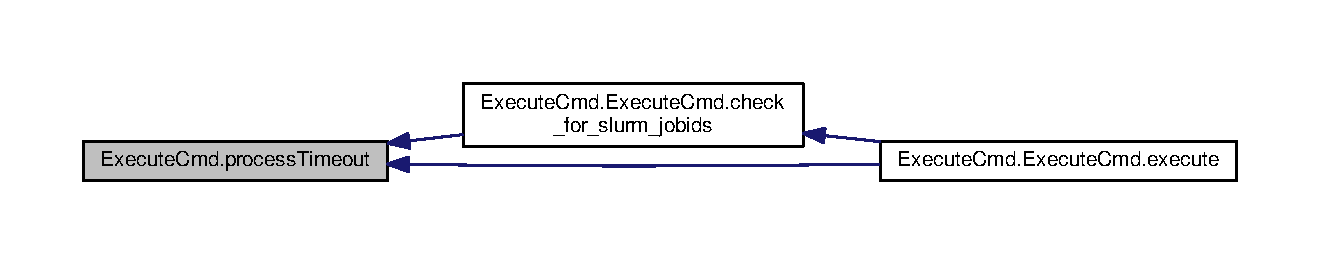
\includegraphics[width=350pt]{namespace_execute_cmd_a656974b86a0748fd2511d5646299dbfe_icgraph}
\end{center}
\end{figure}



\input{namespace_executor_m_t_t_tool}
\input{namespace_fetch_m_t_t_tool}
\hypertarget{namespace_fetch_r_p_m}{\section{Fetch\-R\-P\-M Namespace Reference}
\label{namespace_fetch_r_p_m}\index{Fetch\-R\-P\-M@{Fetch\-R\-P\-M}}
}
\subsection*{Classes}
\begin{DoxyCompactItemize}
\item 
class \hyperlink{class_fetch_r_p_m_1_1_fetch_r_p_m}{Fetch\-R\-P\-M}
\end{DoxyCompactItemize}

\hypertarget{namespace_fetch_tarball}{\section{Fetch\-Tarball Namespace Reference}
\label{namespace_fetch_tarball}\index{Fetch\-Tarball@{Fetch\-Tarball}}
}
\subsection*{Classes}
\begin{DoxyCompactItemize}
\item 
class \hyperlink{class_fetch_tarball_1_1_fetch_tarball}{Fetch\-Tarball}
\end{DoxyCompactItemize}

\input{namespace_firmware_m_t_t_stage}
\input{namespace_foo_flash}
\input{namespace_git}
\input{namespace_harasser}
\input{namespace_harasser_m_t_t_tool}
\input{namespace_hostfile}
\input{namespace_i_p_m_i_tool}
\input{namespace_i_u_database}
\input{namespace_junit_x_m_l}
\input{namespace_launcher_defaults_m_t_t_stage}
\input{namespace_launcher_m_t_t_tool}
\input{namespace_load_classes}
\input{namespace_logger}
\input{namespace_middleware_build_m_t_t_stage}
\input{namespace_middleware_get_m_t_t_stage}
\input{namespace_module_cmd}
\input{namespace_m_p_i_version}
\input{namespace_m_t_t_defaults_m_t_t_stage}
\input{namespace_m_t_t_version_plugin}
\input{namespace_o_m_p_i___snapshot}
\input{namespace_open_m_p_i}
\hypertarget{namespace_pip}{\section{Pip Namespace Reference}
\label{namespace_pip}\index{Pip@{Pip}}
}

\hypertarget{namespace_p_m_ix_unit}{\section{P\-M\-Ix\-Unit Namespace Reference}
\label{namespace_p_m_ix_unit}\index{P\-M\-Ix\-Unit@{P\-M\-Ix\-Unit}}
}

\input{namespace_profile_m_t_t_stage}
\input{namespace_provision_m_t_t_stage}
\hypertarget{namespace_p_r_r_t_e}{\section{P\-R\-R\-T\-E Namespace Reference}
\label{namespace_p_r_r_t_e}\index{P\-R\-R\-T\-E@{P\-R\-R\-T\-E}}
}
\subsection*{Classes}
\begin{DoxyCompactItemize}
\item 
class \hyperlink{class_p_r_r_t_e_1_1_p_r_r_t_e}{P\-R\-R\-T\-E}
\end{DoxyCompactItemize}

\hypertarget{namespacepymtt}{\section{pymtt Namespace Reference}
\label{namespacepymtt}\index{pymtt@{pymtt}}
}
\subsection*{Variables}
\begin{DoxyCompactItemize}
\item 
tuple \hyperlink{namespacepymtt_a95d54fdad48aac280be9d57cf81dee68}{parser}
\item 
tuple \hyperlink{namespacepymtt_a99ad2929ecc4e17f97670bed44f08c35}{info\-Group} = parser.\-add\-\_\-argument\-\_\-group('Info\-Group','Informational Options')
\item 
string \hyperlink{namespacepymtt_a5ee564a034624d925bb8dc823d11c522}{action} = \char`\"{}store\-\_\-true\char`\"{}
\item 
string \hyperlink{namespacepymtt_a21e88c39af91deb569da20633d245b09}{help} = \char`\"{}Print version\char`\"{}
\item 
tuple \hyperlink{namespacepymtt_a0f52dbd5d46583e466305a708dea64a1}{exec\-Group} = parser.\-add\-\_\-argument\-\_\-group('exec\-Group', \char`\"{}Execution Options\char`\"{})
\item 
string \hyperlink{namespacepymtt_a9ecea46ee6082edb9bbdd8393829e18e}{dest} = \char`\"{}duration\char`\"{}
\item 
tuple \hyperlink{namespacepymtt_af066a010075617c13a5595243ceb9041}{debug\-Group} = parser.\-add\-\_\-argument\-\_\-group('debug\-Group', 'Debug Options')
\item 
tuple \hyperlink{namespacepymtt_af7633cc372f3357c4f8e6f8dedfe7a8e}{args} = parser.\-parse\-\_\-args()
\item 
list \hyperlink{namespacepymtt_a7dea31bd26744bab0b1c30dc11c718aa}{mtt\-Args} = \mbox{[}$\,$\mbox{]}
\item 
list \hyperlink{namespacepymtt_a109ef76f074b08666398bf6a38219cfc}{mtthome} = os.\-environ\mbox{[}'M\-T\-T\-\_\-\-H\-O\-M\-E'\mbox{]}
\item 
tuple \hyperlink{namespacepymtt_ac673c895b8c93a029d2a1655c04af315}{topdir} = os.\-path.\-join(\hyperlink{namespacepymtt_a109ef76f074b08666398bf6a38219cfc}{mtthome}, \char`\"{}pylib\char`\"{})
\item 
tuple \hyperlink{namespacepymtt_a57729393cfbd99464570d7fa5ad9fa05}{basedir} = args.\-basediroros.\-path.\-join(\hyperlink{namespacepymtt_a109ef76f074b08666398bf6a38219cfc}{mtthome}, \char`\"{}pylib\char`\"{}, \char`\"{}System\char`\"{})
\item 
tuple \hyperlink{namespacepymtt_ab13a60c31fa69917ce06c1a2631aaf02}{m} = imp.\-load\-\_\-source(\char`\"{}Test\-Def\char`\"{}, os.\-path.\-join(\hyperlink{namespacepymtt_a57729393cfbd99464570d7fa5ad9fa05}{basedir}, \char`\"{}Test\-Def.\-py\char`\"{}))
\item 
tuple \hyperlink{namespacepymtt_a17f658b5d141d51664bb3ede8830c4c0}{cls} = getattr(\hyperlink{namespacepymtt_ab13a60c31fa69917ce06c1a2631aaf02}{m}, \char`\"{}Test\-Def\char`\"{})
\item 
tuple \hyperlink{namespacepymtt_a55825c16c4bd231f7ffbd0fe52407e3f}{a} = \hyperlink{namespacepymtt_a17f658b5d141d51664bb3ede8830c4c0}{cls}()
\item 
tuple \hyperlink{namespacepymtt_afebe539e6104da8ebd3d06b7a0e77fe7}{test\-Def} = a.\-\_\-\-\_\-class\-\_\-\-\_\-()
\item 
string \hyperlink{namespacepymtt_a5d5ee597f85e5c40ec6a923a4398c291}{fallback} = \char`\"{}sequential\char`\"{}
\item 
tuple \hyperlink{namespacepymtt_a283715e769294f7b1362c85498cdf2a3}{executor} = args.\-executorortest\-Def.\-config.\-get('M\-T\-T\-Defaults', 'executor', \hyperlink{namespacepymtt_a5d5ee597f85e5c40ec6a923a4398c291}{fallback}=\hyperlink{namespacepymtt_a5d5ee597f85e5c40ec6a923a4398c291}{fallback})
\item 
tuple \hyperlink{namespacepymtt_a1a2fd13626c1c2d248cedc138e8660ec}{status} = test\-Def.\-execute\-Test(\hyperlink{namespacepymtt_a283715e769294f7b1362c85498cdf2a3}{executor}=executor.\-lower())
\end{DoxyCompactItemize}


\subsection{Variable Documentation}
\hypertarget{namespacepymtt_a55825c16c4bd231f7ffbd0fe52407e3f}{\index{pymtt@{pymtt}!a@{a}}
\index{a@{a}!pymtt@{pymtt}}
\subsubsection[{a}]{\setlength{\rightskip}{0pt plus 5cm}tuple pymtt.\-a = {\bf cls}()}}\label{namespacepymtt_a55825c16c4bd231f7ffbd0fe52407e3f}


Definition at line 222 of file pymtt.\-py.

\hypertarget{namespacepymtt_a5ee564a034624d925bb8dc823d11c522}{\index{pymtt@{pymtt}!action@{action}}
\index{action@{action}!pymtt@{pymtt}}
\subsubsection[{action}]{\setlength{\rightskip}{0pt plus 5cm}string pymtt.\-action = \char`\"{}store\-\_\-true\char`\"{}}}\label{namespacepymtt_a5ee564a034624d925bb8dc823d11c522}


Definition at line 43 of file pymtt.\-py.

\hypertarget{namespacepymtt_af7633cc372f3357c4f8e6f8dedfe7a8e}{\index{pymtt@{pymtt}!args@{args}}
\index{args@{args}!pymtt@{pymtt}}
\subsubsection[{args}]{\setlength{\rightskip}{0pt plus 5cm}tuple pymtt.\-args = parser.\-parse\-\_\-args()}}\label{namespacepymtt_af7633cc372f3357c4f8e6f8dedfe7a8e}


Definition at line 151 of file pymtt.\-py.

\hypertarget{namespacepymtt_a57729393cfbd99464570d7fa5ad9fa05}{\index{pymtt@{pymtt}!basedir@{basedir}}
\index{basedir@{basedir}!pymtt@{pymtt}}
\subsubsection[{basedir}]{\setlength{\rightskip}{0pt plus 5cm}tuple pymtt.\-basedir = args.\-basediroros.\-path.\-join({\bf mtthome}, \char`\"{}pylib\char`\"{}, \char`\"{}System\char`\"{})}}\label{namespacepymtt_a57729393cfbd99464570d7fa5ad9fa05}


Definition at line 198 of file pymtt.\-py.

\hypertarget{namespacepymtt_a17f658b5d141d51664bb3ede8830c4c0}{\index{pymtt@{pymtt}!cls@{cls}}
\index{cls@{cls}!pymtt@{pymtt}}
\subsubsection[{cls}]{\setlength{\rightskip}{0pt plus 5cm}tuple pymtt.\-cls = getattr({\bf m}, \char`\"{}Test\-Def\char`\"{})}}\label{namespacepymtt_a17f658b5d141d51664bb3ede8830c4c0}


Definition at line 221 of file pymtt.\-py.

\hypertarget{namespacepymtt_af066a010075617c13a5595243ceb9041}{\index{pymtt@{pymtt}!debug\-Group@{debug\-Group}}
\index{debug\-Group@{debug\-Group}!pymtt@{pymtt}}
\subsubsection[{debug\-Group}]{\setlength{\rightskip}{0pt plus 5cm}tuple pymtt.\-debug\-Group = parser.\-add\-\_\-argument\-\_\-group('debug\-Group', 'Debug Options')}}\label{namespacepymtt_af066a010075617c13a5595243ceb9041}


Definition at line 135 of file pymtt.\-py.

\hypertarget{namespacepymtt_a9ecea46ee6082edb9bbdd8393829e18e}{\index{pymtt@{pymtt}!dest@{dest}}
\index{dest@{dest}!pymtt@{pymtt}}
\subsubsection[{dest}]{\setlength{\rightskip}{0pt plus 5cm}string pymtt.\-dest = \char`\"{}duration\char`\"{}}}\label{namespacepymtt_a9ecea46ee6082edb9bbdd8393829e18e}


Definition at line 117 of file pymtt.\-py.

\hypertarget{namespacepymtt_a0f52dbd5d46583e466305a708dea64a1}{\index{pymtt@{pymtt}!exec\-Group@{exec\-Group}}
\index{exec\-Group@{exec\-Group}!pymtt@{pymtt}}
\subsubsection[{exec\-Group}]{\setlength{\rightskip}{0pt plus 5cm}tuple pymtt.\-exec\-Group = parser.\-add\-\_\-argument\-\_\-group('exec\-Group', \char`\"{}Execution Options\char`\"{})}}\label{namespacepymtt_a0f52dbd5d46583e466305a708dea64a1}


Definition at line 73 of file pymtt.\-py.

\hypertarget{namespacepymtt_a283715e769294f7b1362c85498cdf2a3}{\index{pymtt@{pymtt}!executor@{executor}}
\index{executor@{executor}!pymtt@{pymtt}}
\subsubsection[{executor}]{\setlength{\rightskip}{0pt plus 5cm}tuple pymtt.\-executor = args.\-executorortest\-Def.\-config.\-get('M\-T\-T\-Defaults', 'executor', {\bf fallback}={\bf fallback})}}\label{namespacepymtt_a283715e769294f7b1362c85498cdf2a3}


Definition at line 256 of file pymtt.\-py.

\hypertarget{namespacepymtt_a5d5ee597f85e5c40ec6a923a4398c291}{\index{pymtt@{pymtt}!fallback@{fallback}}
\index{fallback@{fallback}!pymtt@{pymtt}}
\subsubsection[{fallback}]{\setlength{\rightskip}{0pt plus 5cm}string pymtt.\-fallback = \char`\"{}sequential\char`\"{}}}\label{namespacepymtt_a5d5ee597f85e5c40ec6a923a4398c291}


Definition at line 255 of file pymtt.\-py.

\hypertarget{namespacepymtt_a21e88c39af91deb569da20633d245b09}{\index{pymtt@{pymtt}!help@{help}}
\index{help@{help}!pymtt@{pymtt}}
\subsubsection[{help}]{\setlength{\rightskip}{0pt plus 5cm}string pymtt.\-help = \char`\"{}Print version\char`\"{}}}\label{namespacepymtt_a21e88c39af91deb569da20633d245b09}


Definition at line 44 of file pymtt.\-py.

\hypertarget{namespacepymtt_a99ad2929ecc4e17f97670bed44f08c35}{\index{pymtt@{pymtt}!info\-Group@{info\-Group}}
\index{info\-Group@{info\-Group}!pymtt@{pymtt}}
\subsubsection[{info\-Group}]{\setlength{\rightskip}{0pt plus 5cm}tuple pymtt.\-info\-Group = parser.\-add\-\_\-argument\-\_\-group('Info\-Group','Informational Options')}}\label{namespacepymtt_a99ad2929ecc4e17f97670bed44f08c35}


Definition at line 41 of file pymtt.\-py.

\hypertarget{namespacepymtt_ab13a60c31fa69917ce06c1a2631aaf02}{\index{pymtt@{pymtt}!m@{m}}
\index{m@{m}!pymtt@{pymtt}}
\subsubsection[{m}]{\setlength{\rightskip}{0pt plus 5cm}tuple pymtt.\-m = imp.\-load\-\_\-source(\char`\"{}Test\-Def\char`\"{}, os.\-path.\-join({\bf basedir}, \char`\"{}Test\-Def.\-py\char`\"{}))}}\label{namespacepymtt_ab13a60c31fa69917ce06c1a2631aaf02}


Definition at line 217 of file pymtt.\-py.

\hypertarget{namespacepymtt_a7dea31bd26744bab0b1c30dc11c718aa}{\index{pymtt@{pymtt}!mtt\-Args@{mtt\-Args}}
\index{mtt\-Args@{mtt\-Args}!pymtt@{pymtt}}
\subsubsection[{mtt\-Args}]{\setlength{\rightskip}{0pt plus 5cm}tuple pymtt.\-mtt\-Args = \mbox{[}$\,$\mbox{]}}}\label{namespacepymtt_a7dea31bd26744bab0b1c30dc11c718aa}


Definition at line 155 of file pymtt.\-py.

\hypertarget{namespacepymtt_a109ef76f074b08666398bf6a38219cfc}{\index{pymtt@{pymtt}!mtthome@{mtthome}}
\index{mtthome@{mtthome}!pymtt@{pymtt}}
\subsubsection[{mtthome}]{\setlength{\rightskip}{0pt plus 5cm}list pymtt.\-mtthome = os.\-environ\mbox{[}'M\-T\-T\-\_\-\-H\-O\-M\-E'\mbox{]}}}\label{namespacepymtt_a109ef76f074b08666398bf6a38219cfc}


Definition at line 162 of file pymtt.\-py.

\hypertarget{namespacepymtt_a95d54fdad48aac280be9d57cf81dee68}{\index{pymtt@{pymtt}!parser@{parser}}
\index{parser@{parser}!pymtt@{pymtt}}
\subsubsection[{parser}]{\setlength{\rightskip}{0pt plus 5cm}tuple pymtt.\-parser}}\label{namespacepymtt_a95d54fdad48aac280be9d57cf81dee68}
{\bfseries Initial value\-:}
\begin{DoxyCode}
1 = argparse.ArgumentParser(
2     formatter\_class=argparse.RawDescriptionHelpFormatter,
3     description=\textcolor{stringliteral}{'''\(\backslash\)}
4 \textcolor{stringliteral}{Environment Variables:}
5 \textcolor{stringliteral}{  MTT\_HOME - this must be set to the top-level directory of your MTT installation.}
6 \textcolor{stringliteral}{  MTT\_ARGS - list of commandline arguments that you want set for each invocation.}
7 \textcolor{stringliteral}{    Example: export MTT\_ARGS="--verbose --log=/tmp/out.log"}
8 \textcolor{stringliteral}{'''})
\end{DoxyCode}


Definition at line 30 of file pymtt.\-py.

\hypertarget{namespacepymtt_a1a2fd13626c1c2d248cedc138e8660ec}{\index{pymtt@{pymtt}!status@{status}}
\index{status@{status}!pymtt@{pymtt}}
\subsubsection[{status}]{\setlength{\rightskip}{0pt plus 5cm}tuple pymtt.\-status = test\-Def.\-execute\-Test({\bf executor}=executor.\-lower())}}\label{namespacepymtt_a1a2fd13626c1c2d248cedc138e8660ec}


Definition at line 262 of file pymtt.\-py.

\hypertarget{namespacepymtt_afebe539e6104da8ebd3d06b7a0e77fe7}{\index{pymtt@{pymtt}!test\-Def@{test\-Def}}
\index{test\-Def@{test\-Def}!pymtt@{pymtt}}
\subsubsection[{test\-Def}]{\setlength{\rightskip}{0pt plus 5cm}tuple pymtt.\-test\-Def = a.\-\_\-\-\_\-class\-\_\-\-\_\-()}}\label{namespacepymtt_afebe539e6104da8ebd3d06b7a0e77fe7}


Definition at line 226 of file pymtt.\-py.

\hypertarget{namespacepymtt_ac673c895b8c93a029d2a1655c04af315}{\index{pymtt@{pymtt}!topdir@{topdir}}
\index{topdir@{topdir}!pymtt@{pymtt}}
\subsubsection[{topdir}]{\setlength{\rightskip}{0pt plus 5cm}tuple pymtt.\-topdir = os.\-path.\-join({\bf mtthome}, \char`\"{}pylib\char`\"{})}}\label{namespacepymtt_ac673c895b8c93a029d2a1655c04af315}


Definition at line 184 of file pymtt.\-py.


\input{namespace_reporter_m_t_t_stage}
\hypertarget{namespacesequential}{\section{sequential Namespace Reference}
\label{namespacesequential}\index{sequential@{sequential}}
}
\subsection*{Classes}
\begin{DoxyCompactItemize}
\item 
class \hyperlink{classsequential_1_1_sequential_ex}{Sequential\-Ex}
\end{DoxyCompactItemize}

\input{namespace_shell}
\input{namespace_s_l_u_r_m}
\input{namespacetest___test_def}
\input{namespace_test_build_m_t_t_stage}
\hypertarget{namespace_test_def}{\section{Test\-Def Namespace Reference}
\label{namespace_test_def}\index{Test\-Def@{Test\-Def}}
}
\subsection*{Classes}
\begin{DoxyCompactItemize}
\item 
class \hyperlink{class_test_def_1_1_test_def}{Test\-Def}
\end{DoxyCompactItemize}
\subsection*{Functions}
\begin{DoxyCompactItemize}
\item 
def \hyperlink{namespace_test_def_a0f44619ec0fe932324e50d8cf706d647}{\-\_\-mkdir\-\_\-recursive}
\end{DoxyCompactItemize}
\subsection*{Variables}
\begin{DoxyCompactItemize}
\item 
list \hyperlink{namespace_test_def_a4e87724b7a6a117c2cca22c557936868}{is\-\_\-py2} = sys.\-version\mbox{[}0\mbox{]}
\end{DoxyCompactItemize}


\subsection{Function Documentation}
\hypertarget{namespace_test_def_a0f44619ec0fe932324e50d8cf706d647}{\index{Test\-Def@{Test\-Def}!\-\_\-mkdir\-\_\-recursive@{\-\_\-mkdir\-\_\-recursive}}
\index{\-\_\-mkdir\-\_\-recursive@{\-\_\-mkdir\-\_\-recursive}!TestDef@{Test\-Def}}
\subsubsection[{\-\_\-mkdir\-\_\-recursive}]{\setlength{\rightskip}{0pt plus 5cm}def Test\-Def.\-\_\-mkdir\-\_\-recursive (
\begin{DoxyParamCaption}
\item[{}]{path}
\end{DoxyParamCaption}
)\hspace{0.3cm}{\ttfamily [private]}}}\label{namespace_test_def_a0f44619ec0fe932324e50d8cf706d647}


Definition at line 36 of file Test\-Def.\-py.



\subsection{Variable Documentation}
\hypertarget{namespace_test_def_a4e87724b7a6a117c2cca22c557936868}{\index{Test\-Def@{Test\-Def}!is\-\_\-py2@{is\-\_\-py2}}
\index{is\-\_\-py2@{is\-\_\-py2}!TestDef@{Test\-Def}}
\subsubsection[{is\-\_\-py2}]{\setlength{\rightskip}{0pt plus 5cm}list Test\-Def.\-is\-\_\-py2 = sys.\-version\mbox{[}0\mbox{]}}}\label{namespace_test_def_a4e87724b7a6a117c2cca22c557936868}


Definition at line 29 of file Test\-Def.\-py.


\input{namespace_test_get_m_t_t_stage}
\input{namespace_test_run_m_t_t_stage}
\input{namespace_text_file}
\input{namespace_version_m_t_t_tool}
\input{namespace_watchdog}
\input{namespace_w_wulf3}
\chapter{Class Documentation}
\hypertarget{class_a_l_p_s_1_1_a_l_p_s}{\section{A\-L\-P\-S.\-A\-L\-P\-S Class Reference}
\label{class_a_l_p_s_1_1_a_l_p_s}\index{A\-L\-P\-S.\-A\-L\-P\-S@{A\-L\-P\-S.\-A\-L\-P\-S}}
}


Inheritance diagram for A\-L\-P\-S.\-A\-L\-P\-S\-:
\nopagebreak
\begin{figure}[H]
\begin{center}
\leavevmode
\includegraphics[width=218pt]{class_a_l_p_s_1_1_a_l_p_s__inherit__graph}
\end{center}
\end{figure}


Collaboration diagram for A\-L\-P\-S.\-A\-L\-P\-S\-:
\nopagebreak
\begin{figure}[H]
\begin{center}
\leavevmode
\includegraphics[width=218pt]{class_a_l_p_s_1_1_a_l_p_s__coll__graph}
\end{center}
\end{figure}
\subsection*{Public Member Functions}
\begin{DoxyCompactItemize}
\item 
def \hyperlink{class_a_l_p_s_1_1_a_l_p_s_a45417f6290435c66b3f3b7c4586915d9}{\-\_\-\-\_\-init\-\_\-\-\_\-}
\item 
def \hyperlink{class_a_l_p_s_1_1_a_l_p_s_a3d507bd3feb505c8ed1b4e8f3729d636}{activate}
\item 
def \hyperlink{class_a_l_p_s_1_1_a_l_p_s_aa1d63291a23bcca8ccbd44dc4d0fa6bf}{deactivate}
\item 
def \hyperlink{class_a_l_p_s_1_1_a_l_p_s_a97e56ee7f5faaea26121d6ee0deeddab}{print\-\_\-name}
\item 
def \hyperlink{class_a_l_p_s_1_1_a_l_p_s_a68c17d876ad850e44d40aa082b674f4e}{print\-\_\-options}
\item 
def \hyperlink{class_a_l_p_s_1_1_a_l_p_s_af4b8efc64ea3abc5fb21fb93bfe052ff}{execute}
\end{DoxyCompactItemize}
\subsection*{Public Attributes}
\begin{DoxyCompactItemize}
\item 
\hyperlink{class_a_l_p_s_1_1_a_l_p_s_a24dfa9b508f507c4cb6148f10a081555}{options}
\item 
\hyperlink{class_a_l_p_s_1_1_a_l_p_s_ac371dce53e8c120f7031259025562bdb}{allocated}
\item 
\hyperlink{class_a_l_p_s_1_1_a_l_p_s_a839c4f84a46683221d51004c08345ff2}{test\-Def}
\item 
\hyperlink{class_a_l_p_s_1_1_a_l_p_s_a64bae95ba692ef4df06f716692b50ee9}{cmds}
\end{DoxyCompactItemize}


\subsection{Detailed Description}


Definition at line 43 of file A\-L\-P\-S.\-py.



\subsection{Constructor \& Destructor Documentation}
\hypertarget{class_a_l_p_s_1_1_a_l_p_s_a45417f6290435c66b3f3b7c4586915d9}{\index{A\-L\-P\-S\-::\-A\-L\-P\-S@{A\-L\-P\-S\-::\-A\-L\-P\-S}!\-\_\-\-\_\-init\-\_\-\-\_\-@{\-\_\-\-\_\-init\-\_\-\-\_\-}}
\index{\-\_\-\-\_\-init\-\_\-\-\_\-@{\-\_\-\-\_\-init\-\_\-\-\_\-}!ALPS::ALPS@{A\-L\-P\-S\-::\-A\-L\-P\-S}}
\subsubsection[{\-\_\-\-\_\-init\-\_\-\-\_\-}]{\setlength{\rightskip}{0pt plus 5cm}def A\-L\-P\-S.\-A\-L\-P\-S.\-\_\-\-\_\-init\-\_\-\-\_\- (
\begin{DoxyParamCaption}
\item[{}]{self}
\end{DoxyParamCaption}
)}}\label{class_a_l_p_s_1_1_a_l_p_s_a45417f6290435c66b3f3b7c4586915d9}


Definition at line 45 of file A\-L\-P\-S.\-py.



\subsection{Member Function Documentation}
\hypertarget{class_a_l_p_s_1_1_a_l_p_s_a3d507bd3feb505c8ed1b4e8f3729d636}{\index{A\-L\-P\-S\-::\-A\-L\-P\-S@{A\-L\-P\-S\-::\-A\-L\-P\-S}!activate@{activate}}
\index{activate@{activate}!ALPS::ALPS@{A\-L\-P\-S\-::\-A\-L\-P\-S}}
\subsubsection[{activate}]{\setlength{\rightskip}{0pt plus 5cm}def A\-L\-P\-S.\-A\-L\-P\-S.\-activate (
\begin{DoxyParamCaption}
\item[{}]{self}
\end{DoxyParamCaption}
)}}\label{class_a_l_p_s_1_1_a_l_p_s_a3d507bd3feb505c8ed1b4e8f3729d636}


Definition at line 77 of file A\-L\-P\-S.\-py.

\hypertarget{class_a_l_p_s_1_1_a_l_p_s_aa1d63291a23bcca8ccbd44dc4d0fa6bf}{\index{A\-L\-P\-S\-::\-A\-L\-P\-S@{A\-L\-P\-S\-::\-A\-L\-P\-S}!deactivate@{deactivate}}
\index{deactivate@{deactivate}!ALPS::ALPS@{A\-L\-P\-S\-::\-A\-L\-P\-S}}
\subsubsection[{deactivate}]{\setlength{\rightskip}{0pt plus 5cm}def A\-L\-P\-S.\-A\-L\-P\-S.\-deactivate (
\begin{DoxyParamCaption}
\item[{}]{self}
\end{DoxyParamCaption}
)}}\label{class_a_l_p_s_1_1_a_l_p_s_aa1d63291a23bcca8ccbd44dc4d0fa6bf}


Definition at line 83 of file A\-L\-P\-S.\-py.



Here is the call graph for this function\-:
\nopagebreak
\begin{figure}[H]
\begin{center}
\leavevmode
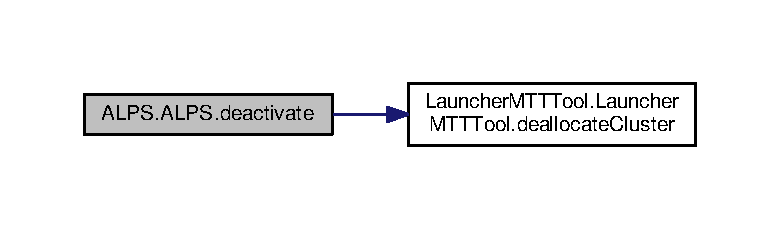
\includegraphics[width=350pt]{class_a_l_p_s_1_1_a_l_p_s_aa1d63291a23bcca8ccbd44dc4d0fa6bf_cgraph}
\end{center}
\end{figure}


\hypertarget{class_a_l_p_s_1_1_a_l_p_s_af4b8efc64ea3abc5fb21fb93bfe052ff}{\index{A\-L\-P\-S\-::\-A\-L\-P\-S@{A\-L\-P\-S\-::\-A\-L\-P\-S}!execute@{execute}}
\index{execute@{execute}!ALPS::ALPS@{A\-L\-P\-S\-::\-A\-L\-P\-S}}
\subsubsection[{execute}]{\setlength{\rightskip}{0pt plus 5cm}def A\-L\-P\-S.\-A\-L\-P\-S.\-execute (
\begin{DoxyParamCaption}
\item[{}]{self, }
\item[{}]{log, }
\item[{}]{keyvals, }
\item[{}]{test\-Def}
\end{DoxyParamCaption}
)}}\label{class_a_l_p_s_1_1_a_l_p_s_af4b8efc64ea3abc5fb21fb93bfe052ff}


Definition at line 99 of file A\-L\-P\-S.\-py.



Here is the call graph for this function\-:
\nopagebreak
\begin{figure}[H]
\begin{center}
\leavevmode
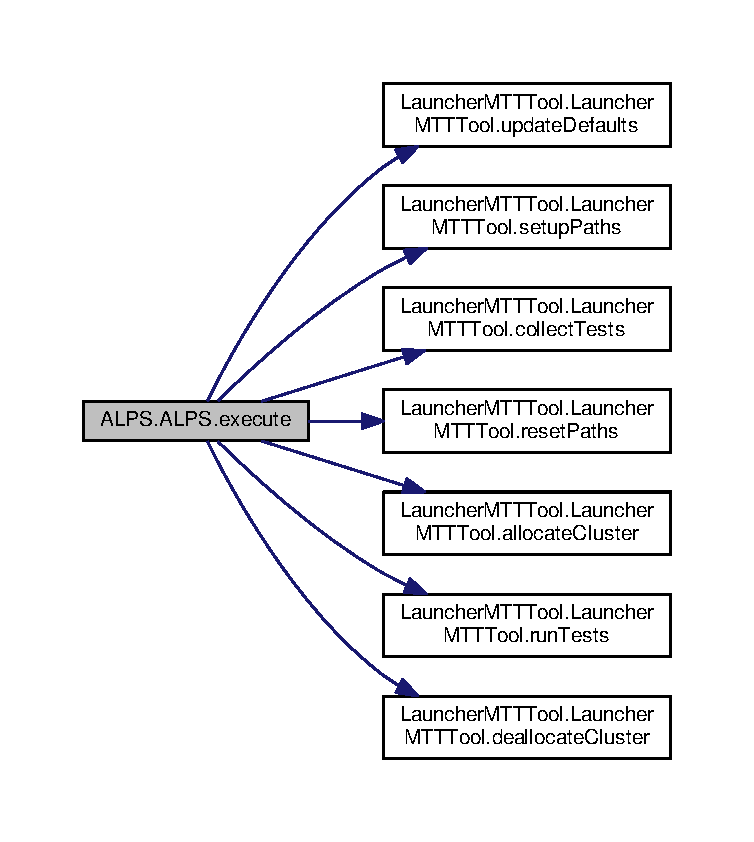
\includegraphics[width=350pt]{class_a_l_p_s_1_1_a_l_p_s_af4b8efc64ea3abc5fb21fb93bfe052ff_cgraph}
\end{center}
\end{figure}


\hypertarget{class_a_l_p_s_1_1_a_l_p_s_a97e56ee7f5faaea26121d6ee0deeddab}{\index{A\-L\-P\-S\-::\-A\-L\-P\-S@{A\-L\-P\-S\-::\-A\-L\-P\-S}!print\-\_\-name@{print\-\_\-name}}
\index{print\-\_\-name@{print\-\_\-name}!ALPS::ALPS@{A\-L\-P\-S\-::\-A\-L\-P\-S}}
\subsubsection[{print\-\_\-name}]{\setlength{\rightskip}{0pt plus 5cm}def A\-L\-P\-S.\-A\-L\-P\-S.\-print\-\_\-name (
\begin{DoxyParamCaption}
\item[{}]{self}
\end{DoxyParamCaption}
)}}\label{class_a_l_p_s_1_1_a_l_p_s_a97e56ee7f5faaea26121d6ee0deeddab}


Definition at line 90 of file A\-L\-P\-S.\-py.

\hypertarget{class_a_l_p_s_1_1_a_l_p_s_a68c17d876ad850e44d40aa082b674f4e}{\index{A\-L\-P\-S\-::\-A\-L\-P\-S@{A\-L\-P\-S\-::\-A\-L\-P\-S}!print\-\_\-options@{print\-\_\-options}}
\index{print\-\_\-options@{print\-\_\-options}!ALPS::ALPS@{A\-L\-P\-S\-::\-A\-L\-P\-S}}
\subsubsection[{print\-\_\-options}]{\setlength{\rightskip}{0pt plus 5cm}def A\-L\-P\-S.\-A\-L\-P\-S.\-print\-\_\-options (
\begin{DoxyParamCaption}
\item[{}]{self, }
\item[{}]{test\-Def, }
\item[{}]{prefix}
\end{DoxyParamCaption}
)}}\label{class_a_l_p_s_1_1_a_l_p_s_a68c17d876ad850e44d40aa082b674f4e}


Definition at line 93 of file A\-L\-P\-S.\-py.



\subsection{Member Data Documentation}
\hypertarget{class_a_l_p_s_1_1_a_l_p_s_ac371dce53e8c120f7031259025562bdb}{\index{A\-L\-P\-S\-::\-A\-L\-P\-S@{A\-L\-P\-S\-::\-A\-L\-P\-S}!allocated@{allocated}}
\index{allocated@{allocated}!ALPS::ALPS@{A\-L\-P\-S\-::\-A\-L\-P\-S}}
\subsubsection[{allocated}]{\setlength{\rightskip}{0pt plus 5cm}A\-L\-P\-S.\-A\-L\-P\-S.\-allocated}}\label{class_a_l_p_s_1_1_a_l_p_s_ac371dce53e8c120f7031259025562bdb}


Definition at line 71 of file A\-L\-P\-S.\-py.

\hypertarget{class_a_l_p_s_1_1_a_l_p_s_a64bae95ba692ef4df06f716692b50ee9}{\index{A\-L\-P\-S\-::\-A\-L\-P\-S@{A\-L\-P\-S\-::\-A\-L\-P\-S}!cmds@{cmds}}
\index{cmds@{cmds}!ALPS::ALPS@{A\-L\-P\-S\-::\-A\-L\-P\-S}}
\subsubsection[{cmds}]{\setlength{\rightskip}{0pt plus 5cm}A\-L\-P\-S.\-A\-L\-P\-S.\-cmds}}\label{class_a_l_p_s_1_1_a_l_p_s_a64bae95ba692ef4df06f716692b50ee9}


Definition at line 73 of file A\-L\-P\-S.\-py.

\hypertarget{class_a_l_p_s_1_1_a_l_p_s_a24dfa9b508f507c4cb6148f10a081555}{\index{A\-L\-P\-S\-::\-A\-L\-P\-S@{A\-L\-P\-S\-::\-A\-L\-P\-S}!options@{options}}
\index{options@{options}!ALPS::ALPS@{A\-L\-P\-S\-::\-A\-L\-P\-S}}
\subsubsection[{options}]{\setlength{\rightskip}{0pt plus 5cm}A\-L\-P\-S.\-A\-L\-P\-S.\-options}}\label{class_a_l_p_s_1_1_a_l_p_s_a24dfa9b508f507c4cb6148f10a081555}


Definition at line 48 of file A\-L\-P\-S.\-py.

\hypertarget{class_a_l_p_s_1_1_a_l_p_s_a839c4f84a46683221d51004c08345ff2}{\index{A\-L\-P\-S\-::\-A\-L\-P\-S@{A\-L\-P\-S\-::\-A\-L\-P\-S}!test\-Def@{test\-Def}}
\index{test\-Def@{test\-Def}!ALPS::ALPS@{A\-L\-P\-S\-::\-A\-L\-P\-S}}
\subsubsection[{test\-Def}]{\setlength{\rightskip}{0pt plus 5cm}A\-L\-P\-S.\-A\-L\-P\-S.\-test\-Def}}\label{class_a_l_p_s_1_1_a_l_p_s_a839c4f84a46683221d51004c08345ff2}


Definition at line 72 of file A\-L\-P\-S.\-py.



The documentation for this class was generated from the following file\-:\begin{DoxyCompactItemize}
\item 
/home/travis/build/open-\/mpi/mtt/pylib/\-Tools/\-Launcher/\hyperlink{_a_l_p_s_8py}{A\-L\-P\-S.\-py}\end{DoxyCompactItemize}

\input{class_already_installed_1_1_already_installed}
\hypertarget{class_autotools_1_1_autotools}{\section{Autotools.\-Autotools Class Reference}
\label{class_autotools_1_1_autotools}\index{Autotools.\-Autotools@{Autotools.\-Autotools}}
}


Inheritance diagram for Autotools.\-Autotools\-:
\nopagebreak
\begin{figure}[H]
\begin{center}
\leavevmode
\includegraphics[width=220pt]{class_autotools_1_1_autotools__inherit__graph}
\end{center}
\end{figure}


Collaboration diagram for Autotools.\-Autotools\-:
\nopagebreak
\begin{figure}[H]
\begin{center}
\leavevmode
\includegraphics[width=220pt]{class_autotools_1_1_autotools__coll__graph}
\end{center}
\end{figure}
\subsection*{Public Member Functions}
\begin{DoxyCompactItemize}
\item 
def \hyperlink{group___tools_ga5b5ac092ad7f4bc45bf785633c8be95a}{\-\_\-\-\_\-init\-\_\-\-\_\-}
\item 
def \hyperlink{group___tools_ga202b0e727db575d20a381cd039dd3597}{activate}
\item 
def \hyperlink{group___tools_ga74513a2f4135b506e66c047559f9571e}{deactivate}
\item 
def \hyperlink{group___tools_ga0873459245ef2255a5a7386957fa592e}{print\-\_\-name}
\item 
def \hyperlink{group___tools_ga41481e9f2a7e7fce32f51cc8feb909fd}{print\-\_\-options}
\item 
def \hyperlink{group___tools_ga5ae85e70e9e6252f4be23ef60624f633}{execute}
\end{DoxyCompactItemize}
\subsection*{Public Attributes}
\begin{DoxyCompactItemize}
\item 
\hyperlink{group___tools_ga6bbb714a91bc8b6fe749326772b073b3}{activated}
\item 
\hyperlink{group___tools_ga8b348e19f0a7104bde9c43c3a6ed695d}{options}
\item 
\hyperlink{group___tools_gaee37d9789ea22ee310ebc357cd721b7f}{exclude}
\end{DoxyCompactItemize}


\subsection{Detailed Description}


Definition at line 42 of file Autotools.\-py.



The documentation for this class was generated from the following file\-:\begin{DoxyCompactItemize}
\item 
/home/travis/build/open-\/mpi/mtt/pylib/\-Tools/\-Build/\hyperlink{_autotools_8py}{Autotools.\-py}\end{DoxyCompactItemize}

\input{class_base_m_t_t_utility_1_1_base_m_t_t_utility}
\input{class_b_i_o_s_m_t_t_stage_1_1_b_i_o_s_m_t_t_stage}
\input{class_build_m_t_t_tool_1_1_build_m_t_t_tool}
\input{class_check_profile_1_1_check_profile}
\input{class_c_n_c_m_t_t_tool_1_1_c_n_c_m_t_t_tool}
\hypertarget{classcombinatorial_1_1_combinatorial_ex}{\section{combinatorial.\-Combinatorial\-Ex Class Reference}
\label{classcombinatorial_1_1_combinatorial_ex}\index{combinatorial.\-Combinatorial\-Ex@{combinatorial.\-Combinatorial\-Ex}}
}


Inheritance diagram for combinatorial.\-Combinatorial\-Ex\-:
\nopagebreak
\begin{figure}[H]
\begin{center}
\leavevmode
\includegraphics[width=228pt]{classcombinatorial_1_1_combinatorial_ex__inherit__graph}
\end{center}
\end{figure}


Collaboration diagram for combinatorial.\-Combinatorial\-Ex\-:
\nopagebreak
\begin{figure}[H]
\begin{center}
\leavevmode
\includegraphics[width=228pt]{classcombinatorial_1_1_combinatorial_ex__coll__graph}
\end{center}
\end{figure}
\subsection*{Public Member Functions}
\begin{DoxyCompactItemize}
\item 
def \hyperlink{classcombinatorial_1_1_combinatorial_ex_a9a4fbfcf64b1204c14509d348dd23b5d}{\-\_\-\-\_\-init\-\_\-\-\_\-}
\item 
def \hyperlink{classcombinatorial_1_1_combinatorial_ex_a8d0b7c0da355183d8124871bee76b0bd}{activate}
\item 
def \hyperlink{classcombinatorial_1_1_combinatorial_ex_ad53efcff93773cce7ed9cfc2fef38ab3}{deactivate}
\item 
def \hyperlink{classcombinatorial_1_1_combinatorial_ex_a19f6321bf42ab92280c5e3b0a3af89d0}{print\-\_\-name}
\item 
def \hyperlink{classcombinatorial_1_1_combinatorial_ex_ae802ad33a050ada42292e7c80fb3e486}{print\-\_\-options}
\item 
def \hyperlink{classcombinatorial_1_1_combinatorial_ex_ac0216f0d0041c35a91e01ac9dafd49da}{create\-Ini\-Log}
\item 
def \hyperlink{classcombinatorial_1_1_combinatorial_ex_a5a5fbd1692c100374ee458e4babc9832}{execute}
\end{DoxyCompactItemize}
\subsection*{Public Attributes}
\begin{DoxyCompactItemize}
\item 
\hyperlink{classcombinatorial_1_1_combinatorial_ex_a20eda525b3947495bb6084c560dcca27}{options}
\item 
\hyperlink{classcombinatorial_1_1_combinatorial_ex_ab5c27fece8991a34f47e85870637fc91}{parser}
\item 
\hyperlink{classcombinatorial_1_1_combinatorial_ex_a24b3bc621a8380e406bade192bc371d4}{temp\-Dir}
\item 
\hyperlink{classcombinatorial_1_1_combinatorial_ex_a68e6ac6cba4ab4161dd854323e549afd}{base\-Ini\-File}
\item 
\hyperlink{classcombinatorial_1_1_combinatorial_ex_a3de3f7da4c201525da8452258df0bc7b}{run\-Log}
\item 
\hyperlink{classcombinatorial_1_1_combinatorial_ex_a961a46d05fda7be52ea74a5f69df57e2}{ini\-Log}
\end{DoxyCompactItemize}


\subsection{Detailed Description}


Definition at line 31 of file combinatorial.\-py.



\subsection{Constructor \& Destructor Documentation}
\hypertarget{classcombinatorial_1_1_combinatorial_ex_a9a4fbfcf64b1204c14509d348dd23b5d}{\index{combinatorial\-::\-Combinatorial\-Ex@{combinatorial\-::\-Combinatorial\-Ex}!\-\_\-\-\_\-init\-\_\-\-\_\-@{\-\_\-\-\_\-init\-\_\-\-\_\-}}
\index{\-\_\-\-\_\-init\-\_\-\-\_\-@{\-\_\-\-\_\-init\-\_\-\-\_\-}!combinatorial::CombinatorialEx@{combinatorial\-::\-Combinatorial\-Ex}}
\subsubsection[{\-\_\-\-\_\-init\-\_\-\-\_\-}]{\setlength{\rightskip}{0pt plus 5cm}def combinatorial.\-Combinatorial\-Ex.\-\_\-\-\_\-init\-\_\-\-\_\- (
\begin{DoxyParamCaption}
\item[{}]{self}
\end{DoxyParamCaption}
)}}\label{classcombinatorial_1_1_combinatorial_ex_a9a4fbfcf64b1204c14509d348dd23b5d}


Definition at line 33 of file combinatorial.\-py.



\subsection{Member Function Documentation}
\hypertarget{classcombinatorial_1_1_combinatorial_ex_a8d0b7c0da355183d8124871bee76b0bd}{\index{combinatorial\-::\-Combinatorial\-Ex@{combinatorial\-::\-Combinatorial\-Ex}!activate@{activate}}
\index{activate@{activate}!combinatorial::CombinatorialEx@{combinatorial\-::\-Combinatorial\-Ex}}
\subsubsection[{activate}]{\setlength{\rightskip}{0pt plus 5cm}def combinatorial.\-Combinatorial\-Ex.\-activate (
\begin{DoxyParamCaption}
\item[{}]{self}
\end{DoxyParamCaption}
)}}\label{classcombinatorial_1_1_combinatorial_ex_a8d0b7c0da355183d8124871bee76b0bd}


Definition at line 45 of file combinatorial.\-py.

\hypertarget{classcombinatorial_1_1_combinatorial_ex_ac0216f0d0041c35a91e01ac9dafd49da}{\index{combinatorial\-::\-Combinatorial\-Ex@{combinatorial\-::\-Combinatorial\-Ex}!create\-Ini\-Log@{create\-Ini\-Log}}
\index{create\-Ini\-Log@{create\-Ini\-Log}!combinatorial::CombinatorialEx@{combinatorial\-::\-Combinatorial\-Ex}}
\subsubsection[{create\-Ini\-Log}]{\setlength{\rightskip}{0pt plus 5cm}def combinatorial.\-Combinatorial\-Ex.\-create\-Ini\-Log (
\begin{DoxyParamCaption}
\item[{}]{self, }
\item[{}]{test\-Def}
\end{DoxyParamCaption}
)}}\label{classcombinatorial_1_1_combinatorial_ex_ac0216f0d0041c35a91e01ac9dafd49da}


Definition at line 66 of file combinatorial.\-py.



Here is the caller graph for this function\-:
\nopagebreak
\begin{figure}[H]
\begin{center}
\leavevmode
\includegraphics[width=350pt]{classcombinatorial_1_1_combinatorial_ex_ac0216f0d0041c35a91e01ac9dafd49da_icgraph}
\end{center}
\end{figure}


\hypertarget{classcombinatorial_1_1_combinatorial_ex_ad53efcff93773cce7ed9cfc2fef38ab3}{\index{combinatorial\-::\-Combinatorial\-Ex@{combinatorial\-::\-Combinatorial\-Ex}!deactivate@{deactivate}}
\index{deactivate@{deactivate}!combinatorial::CombinatorialEx@{combinatorial\-::\-Combinatorial\-Ex}}
\subsubsection[{deactivate}]{\setlength{\rightskip}{0pt plus 5cm}def combinatorial.\-Combinatorial\-Ex.\-deactivate (
\begin{DoxyParamCaption}
\item[{}]{self}
\end{DoxyParamCaption}
)}}\label{classcombinatorial_1_1_combinatorial_ex_ad53efcff93773cce7ed9cfc2fef38ab3}


Definition at line 50 of file combinatorial.\-py.

\hypertarget{classcombinatorial_1_1_combinatorial_ex_a5a5fbd1692c100374ee458e4babc9832}{\index{combinatorial\-::\-Combinatorial\-Ex@{combinatorial\-::\-Combinatorial\-Ex}!execute@{execute}}
\index{execute@{execute}!combinatorial::CombinatorialEx@{combinatorial\-::\-Combinatorial\-Ex}}
\subsubsection[{execute}]{\setlength{\rightskip}{0pt plus 5cm}def combinatorial.\-Combinatorial\-Ex.\-execute (
\begin{DoxyParamCaption}
\item[{}]{self, }
\item[{}]{test\-Def}
\end{DoxyParamCaption}
)}}\label{classcombinatorial_1_1_combinatorial_ex_a5a5fbd1692c100374ee458e4babc9832}


Definition at line 169 of file combinatorial.\-py.



Here is the call graph for this function\-:
\nopagebreak
\begin{figure}[H]
\begin{center}
\leavevmode
\includegraphics[width=350pt]{classcombinatorial_1_1_combinatorial_ex_a5a5fbd1692c100374ee458e4babc9832_cgraph}
\end{center}
\end{figure}


\hypertarget{classcombinatorial_1_1_combinatorial_ex_a19f6321bf42ab92280c5e3b0a3af89d0}{\index{combinatorial\-::\-Combinatorial\-Ex@{combinatorial\-::\-Combinatorial\-Ex}!print\-\_\-name@{print\-\_\-name}}
\index{print\-\_\-name@{print\-\_\-name}!combinatorial::CombinatorialEx@{combinatorial\-::\-Combinatorial\-Ex}}
\subsubsection[{print\-\_\-name}]{\setlength{\rightskip}{0pt plus 5cm}def combinatorial.\-Combinatorial\-Ex.\-print\-\_\-name (
\begin{DoxyParamCaption}
\item[{}]{self}
\end{DoxyParamCaption}
)}}\label{classcombinatorial_1_1_combinatorial_ex_a19f6321bf42ab92280c5e3b0a3af89d0}


Definition at line 54 of file combinatorial.\-py.

\hypertarget{classcombinatorial_1_1_combinatorial_ex_ae802ad33a050ada42292e7c80fb3e486}{\index{combinatorial\-::\-Combinatorial\-Ex@{combinatorial\-::\-Combinatorial\-Ex}!print\-\_\-options@{print\-\_\-options}}
\index{print\-\_\-options@{print\-\_\-options}!combinatorial::CombinatorialEx@{combinatorial\-::\-Combinatorial\-Ex}}
\subsubsection[{print\-\_\-options}]{\setlength{\rightskip}{0pt plus 5cm}def combinatorial.\-Combinatorial\-Ex.\-print\-\_\-options (
\begin{DoxyParamCaption}
\item[{}]{self, }
\item[{}]{test\-Def, }
\item[{}]{prefix}
\end{DoxyParamCaption}
)}}\label{classcombinatorial_1_1_combinatorial_ex_ae802ad33a050ada42292e7c80fb3e486}


Definition at line 57 of file combinatorial.\-py.



\subsection{Member Data Documentation}
\hypertarget{classcombinatorial_1_1_combinatorial_ex_a68e6ac6cba4ab4161dd854323e549afd}{\index{combinatorial\-::\-Combinatorial\-Ex@{combinatorial\-::\-Combinatorial\-Ex}!base\-Ini\-File@{base\-Ini\-File}}
\index{base\-Ini\-File@{base\-Ini\-File}!combinatorial::CombinatorialEx@{combinatorial\-::\-Combinatorial\-Ex}}
\subsubsection[{base\-Ini\-File}]{\setlength{\rightskip}{0pt plus 5cm}combinatorial.\-Combinatorial\-Ex.\-base\-Ini\-File}}\label{classcombinatorial_1_1_combinatorial_ex_a68e6ac6cba4ab4161dd854323e549afd}


Definition at line 41 of file combinatorial.\-py.

\hypertarget{classcombinatorial_1_1_combinatorial_ex_a961a46d05fda7be52ea74a5f69df57e2}{\index{combinatorial\-::\-Combinatorial\-Ex@{combinatorial\-::\-Combinatorial\-Ex}!ini\-Log@{ini\-Log}}
\index{ini\-Log@{ini\-Log}!combinatorial::CombinatorialEx@{combinatorial\-::\-Combinatorial\-Ex}}
\subsubsection[{ini\-Log}]{\setlength{\rightskip}{0pt plus 5cm}combinatorial.\-Combinatorial\-Ex.\-ini\-Log}}\label{classcombinatorial_1_1_combinatorial_ex_a961a46d05fda7be52ea74a5f69df57e2}


Definition at line 43 of file combinatorial.\-py.

\hypertarget{classcombinatorial_1_1_combinatorial_ex_a20eda525b3947495bb6084c560dcca27}{\index{combinatorial\-::\-Combinatorial\-Ex@{combinatorial\-::\-Combinatorial\-Ex}!options@{options}}
\index{options@{options}!combinatorial::CombinatorialEx@{combinatorial\-::\-Combinatorial\-Ex}}
\subsubsection[{options}]{\setlength{\rightskip}{0pt plus 5cm}combinatorial.\-Combinatorial\-Ex.\-options}}\label{classcombinatorial_1_1_combinatorial_ex_a20eda525b3947495bb6084c560dcca27}


Definition at line 36 of file combinatorial.\-py.

\hypertarget{classcombinatorial_1_1_combinatorial_ex_ab5c27fece8991a34f47e85870637fc91}{\index{combinatorial\-::\-Combinatorial\-Ex@{combinatorial\-::\-Combinatorial\-Ex}!parser@{parser}}
\index{parser@{parser}!combinatorial::CombinatorialEx@{combinatorial\-::\-Combinatorial\-Ex}}
\subsubsection[{parser}]{\setlength{\rightskip}{0pt plus 5cm}combinatorial.\-Combinatorial\-Ex.\-parser}}\label{classcombinatorial_1_1_combinatorial_ex_ab5c27fece8991a34f47e85870637fc91}


Definition at line 37 of file combinatorial.\-py.

\hypertarget{classcombinatorial_1_1_combinatorial_ex_a3de3f7da4c201525da8452258df0bc7b}{\index{combinatorial\-::\-Combinatorial\-Ex@{combinatorial\-::\-Combinatorial\-Ex}!run\-Log@{run\-Log}}
\index{run\-Log@{run\-Log}!combinatorial::CombinatorialEx@{combinatorial\-::\-Combinatorial\-Ex}}
\subsubsection[{run\-Log}]{\setlength{\rightskip}{0pt plus 5cm}combinatorial.\-Combinatorial\-Ex.\-run\-Log}}\label{classcombinatorial_1_1_combinatorial_ex_a3de3f7da4c201525da8452258df0bc7b}


Definition at line 42 of file combinatorial.\-py.

\hypertarget{classcombinatorial_1_1_combinatorial_ex_a24b3bc621a8380e406bade192bc371d4}{\index{combinatorial\-::\-Combinatorial\-Ex@{combinatorial\-::\-Combinatorial\-Ex}!temp\-Dir@{temp\-Dir}}
\index{temp\-Dir@{temp\-Dir}!combinatorial::CombinatorialEx@{combinatorial\-::\-Combinatorial\-Ex}}
\subsubsection[{temp\-Dir}]{\setlength{\rightskip}{0pt plus 5cm}combinatorial.\-Combinatorial\-Ex.\-temp\-Dir}}\label{classcombinatorial_1_1_combinatorial_ex_a24b3bc621a8380e406bade192bc371d4}


Definition at line 40 of file combinatorial.\-py.



The documentation for this class was generated from the following file\-:\begin{DoxyCompactItemize}
\item 
/home/travis/build/open-\/mpi/mtt/pylib/\-Tools/\-Executor/\hyperlink{combinatorial_8py}{combinatorial.\-py}\end{DoxyCompactItemize}

\input{class_compilers_1_1_compilers}
\hypertarget{class_copy_1_1_copy}{\section{Copy.\-Copy Class Reference}
\label{class_copy_1_1_copy}\index{Copy.\-Copy@{Copy.\-Copy}}
}


Inheritance diagram for Copy.\-Copy\-:
\nopagebreak
\begin{figure}[H]
\begin{center}
\leavevmode
\includegraphics[width=236pt]{class_copy_1_1_copy__inherit__graph}
\end{center}
\end{figure}


Collaboration diagram for Copy.\-Copy\-:
\nopagebreak
\begin{figure}[H]
\begin{center}
\leavevmode
\includegraphics[width=236pt]{class_copy_1_1_copy__coll__graph}
\end{center}
\end{figure}
\subsection*{Public Member Functions}
\begin{DoxyCompactItemize}
\item 
def \hyperlink{class_copy_1_1_copy_ab4ab01df1326525fc1954500089f8cd4}{\-\_\-\-\_\-init\-\_\-\-\_\-}
\item 
def \hyperlink{class_copy_1_1_copy_a17b5b7fedb1e45364abd52400c502e58}{print\-\_\-name}
\item 
def \hyperlink{class_copy_1_1_copy_a4a189542d9e0537e4345ec3e02a5a16c}{print\-\_\-options}
\item 
def \hyperlink{class_copy_1_1_copy_a3822ae662ccd3a455bb673c975f48e97}{execute}
\end{DoxyCompactItemize}
\subsection*{Public Attributes}
\begin{DoxyCompactItemize}
\item 
\hyperlink{class_copy_1_1_copy_ac6c7d7a32af88b3a7068f937e29a9297}{options}
\end{DoxyCompactItemize}


\subsection{Detailed Description}


Definition at line 33 of file Copy.\-py.



\subsection{Constructor \& Destructor Documentation}
\hypertarget{class_copy_1_1_copy_ab4ab01df1326525fc1954500089f8cd4}{\index{Copy\-::\-Copy@{Copy\-::\-Copy}!\-\_\-\-\_\-init\-\_\-\-\_\-@{\-\_\-\-\_\-init\-\_\-\-\_\-}}
\index{\-\_\-\-\_\-init\-\_\-\-\_\-@{\-\_\-\-\_\-init\-\_\-\-\_\-}!Copy::Copy@{Copy\-::\-Copy}}
\subsubsection[{\-\_\-\-\_\-init\-\_\-\-\_\-}]{\setlength{\rightskip}{0pt plus 5cm}def Copy.\-Copy.\-\_\-\-\_\-init\-\_\-\-\_\- (
\begin{DoxyParamCaption}
\item[{}]{self}
\end{DoxyParamCaption}
)}}\label{class_copy_1_1_copy_ab4ab01df1326525fc1954500089f8cd4}


Definition at line 34 of file Copy.\-py.



\subsection{Member Function Documentation}
\hypertarget{class_copy_1_1_copy_a3822ae662ccd3a455bb673c975f48e97}{\index{Copy\-::\-Copy@{Copy\-::\-Copy}!execute@{execute}}
\index{execute@{execute}!Copy::Copy@{Copy\-::\-Copy}}
\subsubsection[{execute}]{\setlength{\rightskip}{0pt plus 5cm}def Copy.\-Copy.\-execute (
\begin{DoxyParamCaption}
\item[{}]{self, }
\item[{}]{log, }
\item[{}]{keyvals, }
\item[{}]{test\-Def}
\end{DoxyParamCaption}
)}}\label{class_copy_1_1_copy_a3822ae662ccd3a455bb673c975f48e97}


Definition at line 49 of file Copy.\-py.

\hypertarget{class_copy_1_1_copy_a17b5b7fedb1e45364abd52400c502e58}{\index{Copy\-::\-Copy@{Copy\-::\-Copy}!print\-\_\-name@{print\-\_\-name}}
\index{print\-\_\-name@{print\-\_\-name}!Copy::Copy@{Copy\-::\-Copy}}
\subsubsection[{print\-\_\-name}]{\setlength{\rightskip}{0pt plus 5cm}def Copy.\-Copy.\-print\-\_\-name (
\begin{DoxyParamCaption}
\item[{}]{self}
\end{DoxyParamCaption}
)}}\label{class_copy_1_1_copy_a17b5b7fedb1e45364abd52400c502e58}


Definition at line 40 of file Copy.\-py.

\hypertarget{class_copy_1_1_copy_a4a189542d9e0537e4345ec3e02a5a16c}{\index{Copy\-::\-Copy@{Copy\-::\-Copy}!print\-\_\-options@{print\-\_\-options}}
\index{print\-\_\-options@{print\-\_\-options}!Copy::Copy@{Copy\-::\-Copy}}
\subsubsection[{print\-\_\-options}]{\setlength{\rightskip}{0pt plus 5cm}def Copy.\-Copy.\-print\-\_\-options (
\begin{DoxyParamCaption}
\item[{}]{self, }
\item[{}]{test\-Def, }
\item[{}]{prefix}
\end{DoxyParamCaption}
)}}\label{class_copy_1_1_copy_a4a189542d9e0537e4345ec3e02a5a16c}


Definition at line 43 of file Copy.\-py.



\subsection{Member Data Documentation}
\hypertarget{class_copy_1_1_copy_ac6c7d7a32af88b3a7068f937e29a9297}{\index{Copy\-::\-Copy@{Copy\-::\-Copy}!options@{options}}
\index{options@{options}!Copy::Copy@{Copy\-::\-Copy}}
\subsubsection[{options}]{\setlength{\rightskip}{0pt plus 5cm}Copy.\-Copy.\-options}}\label{class_copy_1_1_copy_ac6c7d7a32af88b3a7068f937e29a9297}


Definition at line 36 of file Copy.\-py.



The documentation for this class was generated from the following file\-:\begin{DoxyCompactItemize}
\item 
/home/travis/build/open-\/mpi/mtt/pylib/\-Utilities/\hyperlink{_copy_8py}{Copy.\-py}\end{DoxyCompactItemize}

\hypertarget{class_copytree_1_1_copytree}{\section{Copytree.\-Copytree Class Reference}
\label{class_copytree_1_1_copytree}\index{Copytree.\-Copytree@{Copytree.\-Copytree}}
}


Inheritance diagram for Copytree.\-Copytree\-:
\nopagebreak
\begin{figure}[H]
\begin{center}
\leavevmode
\includegraphics[width=236pt]{class_copytree_1_1_copytree__inherit__graph}
\end{center}
\end{figure}


Collaboration diagram for Copytree.\-Copytree\-:
\nopagebreak
\begin{figure}[H]
\begin{center}
\leavevmode
\includegraphics[width=236pt]{class_copytree_1_1_copytree__coll__graph}
\end{center}
\end{figure}
\subsection*{Public Member Functions}
\begin{DoxyCompactItemize}
\item 
def \hyperlink{class_copytree_1_1_copytree_a7dc4242e406f7418ca7e4f0c31b8c524}{\-\_\-\-\_\-init\-\_\-\-\_\-}
\item 
def \hyperlink{class_copytree_1_1_copytree_ae6dbc27735bd3bdcb0113564c50b1c1c}{print\-\_\-name}
\item 
def \hyperlink{class_copytree_1_1_copytree_a34bbcd07e83438b9ec9855065b13a397}{print\-\_\-options}
\item 
def \hyperlink{class_copytree_1_1_copytree_a567584587407c9c6027bd7026e36a366}{execute}
\end{DoxyCompactItemize}
\subsection*{Public Attributes}
\begin{DoxyCompactItemize}
\item 
\hyperlink{class_copytree_1_1_copytree_ab12d2712ffd4aba7ddd4c5ceadec153b}{options}
\end{DoxyCompactItemize}


\subsection{Detailed Description}


Definition at line 33 of file Copytree.\-py.



\subsection{Constructor \& Destructor Documentation}
\hypertarget{class_copytree_1_1_copytree_a7dc4242e406f7418ca7e4f0c31b8c524}{\index{Copytree\-::\-Copytree@{Copytree\-::\-Copytree}!\-\_\-\-\_\-init\-\_\-\-\_\-@{\-\_\-\-\_\-init\-\_\-\-\_\-}}
\index{\-\_\-\-\_\-init\-\_\-\-\_\-@{\-\_\-\-\_\-init\-\_\-\-\_\-}!Copytree::Copytree@{Copytree\-::\-Copytree}}
\subsubsection[{\-\_\-\-\_\-init\-\_\-\-\_\-}]{\setlength{\rightskip}{0pt plus 5cm}def Copytree.\-Copytree.\-\_\-\-\_\-init\-\_\-\-\_\- (
\begin{DoxyParamCaption}
\item[{}]{self}
\end{DoxyParamCaption}
)}}\label{class_copytree_1_1_copytree_a7dc4242e406f7418ca7e4f0c31b8c524}


Definition at line 34 of file Copytree.\-py.



\subsection{Member Function Documentation}
\hypertarget{class_copytree_1_1_copytree_a567584587407c9c6027bd7026e36a366}{\index{Copytree\-::\-Copytree@{Copytree\-::\-Copytree}!execute@{execute}}
\index{execute@{execute}!Copytree::Copytree@{Copytree\-::\-Copytree}}
\subsubsection[{execute}]{\setlength{\rightskip}{0pt plus 5cm}def Copytree.\-Copytree.\-execute (
\begin{DoxyParamCaption}
\item[{}]{self, }
\item[{}]{log, }
\item[{}]{keyvals, }
\item[{}]{test\-Def}
\end{DoxyParamCaption}
)}}\label{class_copytree_1_1_copytree_a567584587407c9c6027bd7026e36a366}


Definition at line 50 of file Copytree.\-py.

\hypertarget{class_copytree_1_1_copytree_ae6dbc27735bd3bdcb0113564c50b1c1c}{\index{Copytree\-::\-Copytree@{Copytree\-::\-Copytree}!print\-\_\-name@{print\-\_\-name}}
\index{print\-\_\-name@{print\-\_\-name}!Copytree::Copytree@{Copytree\-::\-Copytree}}
\subsubsection[{print\-\_\-name}]{\setlength{\rightskip}{0pt plus 5cm}def Copytree.\-Copytree.\-print\-\_\-name (
\begin{DoxyParamCaption}
\item[{}]{self}
\end{DoxyParamCaption}
)}}\label{class_copytree_1_1_copytree_ae6dbc27735bd3bdcb0113564c50b1c1c}


Definition at line 41 of file Copytree.\-py.

\hypertarget{class_copytree_1_1_copytree_a34bbcd07e83438b9ec9855065b13a397}{\index{Copytree\-::\-Copytree@{Copytree\-::\-Copytree}!print\-\_\-options@{print\-\_\-options}}
\index{print\-\_\-options@{print\-\_\-options}!Copytree::Copytree@{Copytree\-::\-Copytree}}
\subsubsection[{print\-\_\-options}]{\setlength{\rightskip}{0pt plus 5cm}def Copytree.\-Copytree.\-print\-\_\-options (
\begin{DoxyParamCaption}
\item[{}]{self, }
\item[{}]{test\-Def, }
\item[{}]{prefix}
\end{DoxyParamCaption}
)}}\label{class_copytree_1_1_copytree_a34bbcd07e83438b9ec9855065b13a397}


Definition at line 44 of file Copytree.\-py.



\subsection{Member Data Documentation}
\hypertarget{class_copytree_1_1_copytree_ab12d2712ffd4aba7ddd4c5ceadec153b}{\index{Copytree\-::\-Copytree@{Copytree\-::\-Copytree}!options@{options}}
\index{options@{options}!Copytree::Copytree@{Copytree\-::\-Copytree}}
\subsubsection[{options}]{\setlength{\rightskip}{0pt plus 5cm}Copytree.\-Copytree.\-options}}\label{class_copytree_1_1_copytree_ab12d2712ffd4aba7ddd4c5ceadec153b}


Definition at line 36 of file Copytree.\-py.



The documentation for this class was generated from the following file\-:\begin{DoxyCompactItemize}
\item 
/home/travis/build/open-\/mpi/mtt/pylib/\-Utilities/\hyperlink{_copytree_8py}{Copytree.\-py}\end{DoxyCompactItemize}

\input{class_default_m_t_t_defaults_1_1_default_m_t_t_defaults}
\input{class_default_profile_1_1_default_profile}
\hypertarget{class_default_test_build_1_1_default_test_build}{\section{Default\-Test\-Build.\-Default\-Test\-Build Class Reference}
\label{class_default_test_build_1_1_default_test_build}\index{Default\-Test\-Build.\-Default\-Test\-Build@{Default\-Test\-Build.\-Default\-Test\-Build}}
}


Inheritance diagram for Default\-Test\-Build.\-Default\-Test\-Build\-:
\nopagebreak
\begin{figure}[H]
\begin{center}
\leavevmode
\includegraphics[width=228pt]{class_default_test_build_1_1_default_test_build__inherit__graph}
\end{center}
\end{figure}


Collaboration diagram for Default\-Test\-Build.\-Default\-Test\-Build\-:
\nopagebreak
\begin{figure}[H]
\begin{center}
\leavevmode
\includegraphics[width=228pt]{class_default_test_build_1_1_default_test_build__coll__graph}
\end{center}
\end{figure}
\subsection*{Public Member Functions}
\begin{DoxyCompactItemize}
\item 
def \hyperlink{class_default_test_build_1_1_default_test_build_a08729e27591861a8c9b61a6b2618ec2f}{\-\_\-\-\_\-init\-\_\-\-\_\-}
\item 
def \hyperlink{class_default_test_build_1_1_default_test_build_a88b530e5d66e5dc310f77087d8744345}{activate}
\item 
def \hyperlink{class_default_test_build_1_1_default_test_build_a3a1fbc64d9a4750d7ecf722fb6bcd1ce}{deactivate}
\item 
def \hyperlink{class_default_test_build_1_1_default_test_build_a391c37a5d652ad857c57ae07b66b0d7e}{print\-\_\-name}
\item 
def \hyperlink{class_default_test_build_1_1_default_test_build_a38238916f0726d3a8e2b352ddc74f424}{print\-\_\-options}
\item 
def \hyperlink{class_default_test_build_1_1_default_test_build_a17ce5f679320871748b5aa3ea3491c28}{execute}
\end{DoxyCompactItemize}
\subsection*{Public Attributes}
\begin{DoxyCompactItemize}
\item 
\hyperlink{class_default_test_build_1_1_default_test_build_a2c22896be00540cc15625e79bc98c9fc}{options}
\end{DoxyCompactItemize}


\subsection{Detailed Description}


Definition at line 31 of file Default\-Test\-Build.\-py.



\subsection{Constructor \& Destructor Documentation}
\hypertarget{class_default_test_build_1_1_default_test_build_a08729e27591861a8c9b61a6b2618ec2f}{\index{Default\-Test\-Build\-::\-Default\-Test\-Build@{Default\-Test\-Build\-::\-Default\-Test\-Build}!\-\_\-\-\_\-init\-\_\-\-\_\-@{\-\_\-\-\_\-init\-\_\-\-\_\-}}
\index{\-\_\-\-\_\-init\-\_\-\-\_\-@{\-\_\-\-\_\-init\-\_\-\-\_\-}!DefaultTestBuild::DefaultTestBuild@{Default\-Test\-Build\-::\-Default\-Test\-Build}}
\subsubsection[{\-\_\-\-\_\-init\-\_\-\-\_\-}]{\setlength{\rightskip}{0pt plus 5cm}def Default\-Test\-Build.\-Default\-Test\-Build.\-\_\-\-\_\-init\-\_\-\-\_\- (
\begin{DoxyParamCaption}
\item[{}]{self}
\end{DoxyParamCaption}
)}}\label{class_default_test_build_1_1_default_test_build_a08729e27591861a8c9b61a6b2618ec2f}


Definition at line 33 of file Default\-Test\-Build.\-py.



\subsection{Member Function Documentation}
\hypertarget{class_default_test_build_1_1_default_test_build_a88b530e5d66e5dc310f77087d8744345}{\index{Default\-Test\-Build\-::\-Default\-Test\-Build@{Default\-Test\-Build\-::\-Default\-Test\-Build}!activate@{activate}}
\index{activate@{activate}!DefaultTestBuild::DefaultTestBuild@{Default\-Test\-Build\-::\-Default\-Test\-Build}}
\subsubsection[{activate}]{\setlength{\rightskip}{0pt plus 5cm}def Default\-Test\-Build.\-Default\-Test\-Build.\-activate (
\begin{DoxyParamCaption}
\item[{}]{self}
\end{DoxyParamCaption}
)}}\label{class_default_test_build_1_1_default_test_build_a88b530e5d66e5dc310f77087d8744345}


Definition at line 48 of file Default\-Test\-Build.\-py.

\hypertarget{class_default_test_build_1_1_default_test_build_a3a1fbc64d9a4750d7ecf722fb6bcd1ce}{\index{Default\-Test\-Build\-::\-Default\-Test\-Build@{Default\-Test\-Build\-::\-Default\-Test\-Build}!deactivate@{deactivate}}
\index{deactivate@{deactivate}!DefaultTestBuild::DefaultTestBuild@{Default\-Test\-Build\-::\-Default\-Test\-Build}}
\subsubsection[{deactivate}]{\setlength{\rightskip}{0pt plus 5cm}def Default\-Test\-Build.\-Default\-Test\-Build.\-deactivate (
\begin{DoxyParamCaption}
\item[{}]{self}
\end{DoxyParamCaption}
)}}\label{class_default_test_build_1_1_default_test_build_a3a1fbc64d9a4750d7ecf722fb6bcd1ce}


Definition at line 54 of file Default\-Test\-Build.\-py.

\hypertarget{class_default_test_build_1_1_default_test_build_a17ce5f679320871748b5aa3ea3491c28}{\index{Default\-Test\-Build\-::\-Default\-Test\-Build@{Default\-Test\-Build\-::\-Default\-Test\-Build}!execute@{execute}}
\index{execute@{execute}!DefaultTestBuild::DefaultTestBuild@{Default\-Test\-Build\-::\-Default\-Test\-Build}}
\subsubsection[{execute}]{\setlength{\rightskip}{0pt plus 5cm}def Default\-Test\-Build.\-Default\-Test\-Build.\-execute (
\begin{DoxyParamCaption}
\item[{}]{self, }
\item[{}]{log, }
\item[{}]{keyvals, }
\item[{}]{test\-Def}
\end{DoxyParamCaption}
)}}\label{class_default_test_build_1_1_default_test_build_a17ce5f679320871748b5aa3ea3491c28}


Definition at line 67 of file Default\-Test\-Build.\-py.

\hypertarget{class_default_test_build_1_1_default_test_build_a391c37a5d652ad857c57ae07b66b0d7e}{\index{Default\-Test\-Build\-::\-Default\-Test\-Build@{Default\-Test\-Build\-::\-Default\-Test\-Build}!print\-\_\-name@{print\-\_\-name}}
\index{print\-\_\-name@{print\-\_\-name}!DefaultTestBuild::DefaultTestBuild@{Default\-Test\-Build\-::\-Default\-Test\-Build}}
\subsubsection[{print\-\_\-name}]{\setlength{\rightskip}{0pt plus 5cm}def Default\-Test\-Build.\-Default\-Test\-Build.\-print\-\_\-name (
\begin{DoxyParamCaption}
\item[{}]{self}
\end{DoxyParamCaption}
)}}\label{class_default_test_build_1_1_default_test_build_a391c37a5d652ad857c57ae07b66b0d7e}


Definition at line 58 of file Default\-Test\-Build.\-py.

\hypertarget{class_default_test_build_1_1_default_test_build_a38238916f0726d3a8e2b352ddc74f424}{\index{Default\-Test\-Build\-::\-Default\-Test\-Build@{Default\-Test\-Build\-::\-Default\-Test\-Build}!print\-\_\-options@{print\-\_\-options}}
\index{print\-\_\-options@{print\-\_\-options}!DefaultTestBuild::DefaultTestBuild@{Default\-Test\-Build\-::\-Default\-Test\-Build}}
\subsubsection[{print\-\_\-options}]{\setlength{\rightskip}{0pt plus 5cm}def Default\-Test\-Build.\-Default\-Test\-Build.\-print\-\_\-options (
\begin{DoxyParamCaption}
\item[{}]{self, }
\item[{}]{test\-Def, }
\item[{}]{prefix}
\end{DoxyParamCaption}
)}}\label{class_default_test_build_1_1_default_test_build_a38238916f0726d3a8e2b352ddc74f424}


Definition at line 61 of file Default\-Test\-Build.\-py.



\subsection{Member Data Documentation}
\hypertarget{class_default_test_build_1_1_default_test_build_a2c22896be00540cc15625e79bc98c9fc}{\index{Default\-Test\-Build\-::\-Default\-Test\-Build@{Default\-Test\-Build\-::\-Default\-Test\-Build}!options@{options}}
\index{options@{options}!DefaultTestBuild::DefaultTestBuild@{Default\-Test\-Build\-::\-Default\-Test\-Build}}
\subsubsection[{options}]{\setlength{\rightskip}{0pt plus 5cm}Default\-Test\-Build.\-Default\-Test\-Build.\-options}}\label{class_default_test_build_1_1_default_test_build_a2c22896be00540cc15625e79bc98c9fc}


Definition at line 36 of file Default\-Test\-Build.\-py.



The documentation for this class was generated from the following file\-:\begin{DoxyCompactItemize}
\item 
/home/travis/build/open-\/mpi/mtt/pylib/\-Stages/\-Test\-Build/\hyperlink{_default_test_build_8py}{Default\-Test\-Build.\-py}\end{DoxyCompactItemize}

\input{class_environ_1_1_environ}
\hypertarget{class_execute_cmd_1_1_execute_cmd}{\section{Execute\-Cmd.\-Execute\-Cmd Class Reference}
\label{class_execute_cmd_1_1_execute_cmd}\index{Execute\-Cmd.\-Execute\-Cmd@{Execute\-Cmd.\-Execute\-Cmd}}
}


Inheritance diagram for Execute\-Cmd.\-Execute\-Cmd\-:
\nopagebreak
\begin{figure}[H]
\begin{center}
\leavevmode
\includegraphics[width=236pt]{class_execute_cmd_1_1_execute_cmd__inherit__graph}
\end{center}
\end{figure}


Collaboration diagram for Execute\-Cmd.\-Execute\-Cmd\-:
\nopagebreak
\begin{figure}[H]
\begin{center}
\leavevmode
\includegraphics[width=236pt]{class_execute_cmd_1_1_execute_cmd__coll__graph}
\end{center}
\end{figure}
\subsection*{Public Member Functions}
\begin{DoxyCompactItemize}
\item 
def \hyperlink{class_execute_cmd_1_1_execute_cmd_ae0e361beb27aac47f2c682418577b375}{\-\_\-\-\_\-init\-\_\-\-\_\-}
\item 
def \hyperlink{class_execute_cmd_1_1_execute_cmd_a9021ad1c3f3ed4460d57d42a8d1f23ef}{print\-\_\-name}
\item 
def \hyperlink{class_execute_cmd_1_1_execute_cmd_a8174353fba2a214e50529b2612e078ff}{print\-\_\-options}
\item 
def \hyperlink{class_execute_cmd_1_1_execute_cmd_abd51ca569e60d044fe278b613459c709}{execute}
\end{DoxyCompactItemize}
\subsection*{Public Attributes}
\begin{DoxyCompactItemize}
\item 
\hyperlink{class_execute_cmd_1_1_execute_cmd_aea248b8edd01b26099f3d45b798a65be}{options}
\end{DoxyCompactItemize}
\subsection*{Private Member Functions}
\begin{DoxyCompactItemize}
\item 
def \hyperlink{class_execute_cmd_1_1_execute_cmd_a4ab1a3d66079bcb8de5a4a436282ab5c}{\-\_\-bool\-\_\-option}
\item 
def \hyperlink{class_execute_cmd_1_1_execute_cmd_a657ac6b5c7779499ce426ba18234824e}{\-\_\-positive\-\_\-int\-\_\-option}
\end{DoxyCompactItemize}


\subsection{Detailed Description}


Definition at line 27 of file Execute\-Cmd.\-py.



\subsection{Constructor \& Destructor Documentation}
\hypertarget{class_execute_cmd_1_1_execute_cmd_ae0e361beb27aac47f2c682418577b375}{\index{Execute\-Cmd\-::\-Execute\-Cmd@{Execute\-Cmd\-::\-Execute\-Cmd}!\-\_\-\-\_\-init\-\_\-\-\_\-@{\-\_\-\-\_\-init\-\_\-\-\_\-}}
\index{\-\_\-\-\_\-init\-\_\-\-\_\-@{\-\_\-\-\_\-init\-\_\-\-\_\-}!ExecuteCmd::ExecuteCmd@{Execute\-Cmd\-::\-Execute\-Cmd}}
\subsubsection[{\-\_\-\-\_\-init\-\_\-\-\_\-}]{\setlength{\rightskip}{0pt plus 5cm}def Execute\-Cmd.\-Execute\-Cmd.\-\_\-\-\_\-init\-\_\-\-\_\- (
\begin{DoxyParamCaption}
\item[{}]{self}
\end{DoxyParamCaption}
)}}\label{class_execute_cmd_1_1_execute_cmd_ae0e361beb27aac47f2c682418577b375}


Definition at line 28 of file Execute\-Cmd.\-py.



\subsection{Member Function Documentation}
\hypertarget{class_execute_cmd_1_1_execute_cmd_a4ab1a3d66079bcb8de5a4a436282ab5c}{\index{Execute\-Cmd\-::\-Execute\-Cmd@{Execute\-Cmd\-::\-Execute\-Cmd}!\-\_\-bool\-\_\-option@{\-\_\-bool\-\_\-option}}
\index{\-\_\-bool\-\_\-option@{\-\_\-bool\-\_\-option}!ExecuteCmd::ExecuteCmd@{Execute\-Cmd\-::\-Execute\-Cmd}}
\subsubsection[{\-\_\-bool\-\_\-option}]{\setlength{\rightskip}{0pt plus 5cm}def Execute\-Cmd.\-Execute\-Cmd.\-\_\-bool\-\_\-option (
\begin{DoxyParamCaption}
\item[{}]{self, }
\item[{}]{options, }
\item[{}]{name}
\end{DoxyParamCaption}
)\hspace{0.3cm}{\ttfamily [private]}}}\label{class_execute_cmd_1_1_execute_cmd_a4ab1a3d66079bcb8de5a4a436282ab5c}


Definition at line 42 of file Execute\-Cmd.\-py.



Here is the caller graph for this function\-:
\nopagebreak
\begin{figure}[H]
\begin{center}
\leavevmode
\includegraphics[width=350pt]{class_execute_cmd_1_1_execute_cmd_a4ab1a3d66079bcb8de5a4a436282ab5c_icgraph}
\end{center}
\end{figure}


\hypertarget{class_execute_cmd_1_1_execute_cmd_a657ac6b5c7779499ce426ba18234824e}{\index{Execute\-Cmd\-::\-Execute\-Cmd@{Execute\-Cmd\-::\-Execute\-Cmd}!\-\_\-positive\-\_\-int\-\_\-option@{\-\_\-positive\-\_\-int\-\_\-option}}
\index{\-\_\-positive\-\_\-int\-\_\-option@{\-\_\-positive\-\_\-int\-\_\-option}!ExecuteCmd::ExecuteCmd@{Execute\-Cmd\-::\-Execute\-Cmd}}
\subsubsection[{\-\_\-positive\-\_\-int\-\_\-option}]{\setlength{\rightskip}{0pt plus 5cm}def Execute\-Cmd.\-Execute\-Cmd.\-\_\-positive\-\_\-int\-\_\-option (
\begin{DoxyParamCaption}
\item[{}]{self, }
\item[{}]{options, }
\item[{}]{name}
\end{DoxyParamCaption}
)\hspace{0.3cm}{\ttfamily [private]}}}\label{class_execute_cmd_1_1_execute_cmd_a657ac6b5c7779499ce426ba18234824e}


Definition at line 55 of file Execute\-Cmd.\-py.



Here is the caller graph for this function\-:
\nopagebreak
\begin{figure}[H]
\begin{center}
\leavevmode
\includegraphics[width=350pt]{class_execute_cmd_1_1_execute_cmd_a657ac6b5c7779499ce426ba18234824e_icgraph}
\end{center}
\end{figure}


\hypertarget{class_execute_cmd_1_1_execute_cmd_abd51ca569e60d044fe278b613459c709}{\index{Execute\-Cmd\-::\-Execute\-Cmd@{Execute\-Cmd\-::\-Execute\-Cmd}!execute@{execute}}
\index{execute@{execute}!ExecuteCmd::ExecuteCmd@{Execute\-Cmd\-::\-Execute\-Cmd}}
\subsubsection[{execute}]{\setlength{\rightskip}{0pt plus 5cm}def Execute\-Cmd.\-Execute\-Cmd.\-execute (
\begin{DoxyParamCaption}
\item[{}]{self, }
\item[{}]{options, }
\item[{}]{cmdargs, }
\item[{}]{test\-Def}
\end{DoxyParamCaption}
)}}\label{class_execute_cmd_1_1_execute_cmd_abd51ca569e60d044fe278b613459c709}


Definition at line 63 of file Execute\-Cmd.\-py.



Here is the call graph for this function\-:
\nopagebreak
\begin{figure}[H]
\begin{center}
\leavevmode
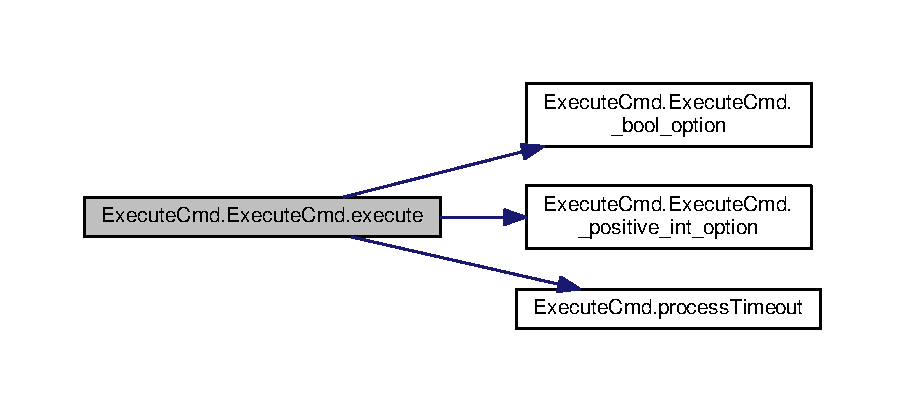
\includegraphics[width=350pt]{class_execute_cmd_1_1_execute_cmd_abd51ca569e60d044fe278b613459c709_cgraph}
\end{center}
\end{figure}


\hypertarget{class_execute_cmd_1_1_execute_cmd_a9021ad1c3f3ed4460d57d42a8d1f23ef}{\index{Execute\-Cmd\-::\-Execute\-Cmd@{Execute\-Cmd\-::\-Execute\-Cmd}!print\-\_\-name@{print\-\_\-name}}
\index{print\-\_\-name@{print\-\_\-name}!ExecuteCmd::ExecuteCmd@{Execute\-Cmd\-::\-Execute\-Cmd}}
\subsubsection[{print\-\_\-name}]{\setlength{\rightskip}{0pt plus 5cm}def Execute\-Cmd.\-Execute\-Cmd.\-print\-\_\-name (
\begin{DoxyParamCaption}
\item[{}]{self}
\end{DoxyParamCaption}
)}}\label{class_execute_cmd_1_1_execute_cmd_a9021ad1c3f3ed4460d57d42a8d1f23ef}


Definition at line 33 of file Execute\-Cmd.\-py.

\hypertarget{class_execute_cmd_1_1_execute_cmd_a8174353fba2a214e50529b2612e078ff}{\index{Execute\-Cmd\-::\-Execute\-Cmd@{Execute\-Cmd\-::\-Execute\-Cmd}!print\-\_\-options@{print\-\_\-options}}
\index{print\-\_\-options@{print\-\_\-options}!ExecuteCmd::ExecuteCmd@{Execute\-Cmd\-::\-Execute\-Cmd}}
\subsubsection[{print\-\_\-options}]{\setlength{\rightskip}{0pt plus 5cm}def Execute\-Cmd.\-Execute\-Cmd.\-print\-\_\-options (
\begin{DoxyParamCaption}
\item[{}]{self, }
\item[{}]{test\-Def, }
\item[{}]{prefix}
\end{DoxyParamCaption}
)}}\label{class_execute_cmd_1_1_execute_cmd_a8174353fba2a214e50529b2612e078ff}


Definition at line 36 of file Execute\-Cmd.\-py.



\subsection{Member Data Documentation}
\hypertarget{class_execute_cmd_1_1_execute_cmd_aea248b8edd01b26099f3d45b798a65be}{\index{Execute\-Cmd\-::\-Execute\-Cmd@{Execute\-Cmd\-::\-Execute\-Cmd}!options@{options}}
\index{options@{options}!ExecuteCmd::ExecuteCmd@{Execute\-Cmd\-::\-Execute\-Cmd}}
\subsubsection[{options}]{\setlength{\rightskip}{0pt plus 5cm}Execute\-Cmd.\-Execute\-Cmd.\-options}}\label{class_execute_cmd_1_1_execute_cmd_aea248b8edd01b26099f3d45b798a65be}


Definition at line 30 of file Execute\-Cmd.\-py.



The documentation for this class was generated from the following file\-:\begin{DoxyCompactItemize}
\item 
/home/travis/build/open-\/mpi/mtt/pylib/\-Utilities/\hyperlink{_execute_cmd_8py}{Execute\-Cmd.\-py}\end{DoxyCompactItemize}

\input{class_executor_m_t_t_tool_1_1_executor_m_t_t_tool}
\input{class_fetch_m_t_t_tool_1_1_fetch_m_t_t_tool}
\hypertarget{class_fetch_r_p_m_1_1_fetch_r_p_m}{\section{Fetch\-R\-P\-M.\-Fetch\-R\-P\-M Class Reference}
\label{class_fetch_r_p_m_1_1_fetch_r_p_m}\index{Fetch\-R\-P\-M.\-Fetch\-R\-P\-M@{Fetch\-R\-P\-M.\-Fetch\-R\-P\-M}}
}


Inheritance diagram for Fetch\-R\-P\-M.\-Fetch\-R\-P\-M\-:
\nopagebreak
\begin{figure}[H]
\begin{center}
\leavevmode
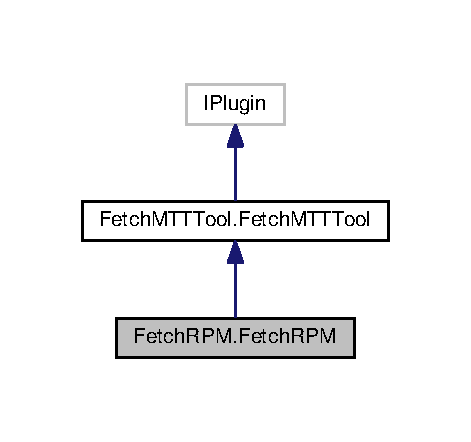
\includegraphics[width=226pt]{class_fetch_r_p_m_1_1_fetch_r_p_m__inherit__graph}
\end{center}
\end{figure}


Collaboration diagram for Fetch\-R\-P\-M.\-Fetch\-R\-P\-M\-:
\nopagebreak
\begin{figure}[H]
\begin{center}
\leavevmode
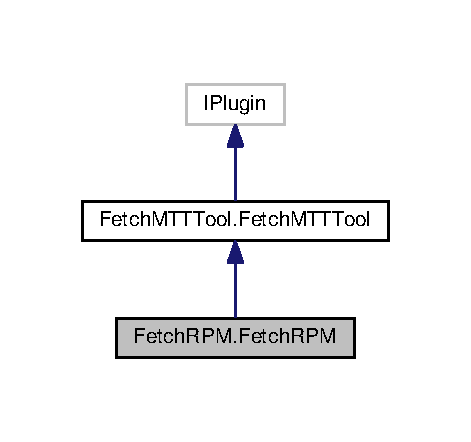
\includegraphics[width=226pt]{class_fetch_r_p_m_1_1_fetch_r_p_m__coll__graph}
\end{center}
\end{figure}
\subsection*{Public Member Functions}
\begin{DoxyCompactItemize}
\item 
def \hyperlink{class_fetch_r_p_m_1_1_fetch_r_p_m_af57a8837250b7782f1b90b2b470193f9}{\-\_\-\-\_\-init\-\_\-\-\_\-}
\item 
def \hyperlink{class_fetch_r_p_m_1_1_fetch_r_p_m_ab8f2446c87e3ea93fd1772eaeb41c1ef}{activate}
\item 
def \hyperlink{class_fetch_r_p_m_1_1_fetch_r_p_m_a7c6c61c0a54efc05bad197921bd8c5b6}{deactivate}
\item 
def \hyperlink{class_fetch_r_p_m_1_1_fetch_r_p_m_a664e74f6ffa5b35fe091774cd9f1bfc1}{print\-\_\-name}
\item 
def \hyperlink{class_fetch_r_p_m_1_1_fetch_r_p_m_aa39b706480033877a1d419f7c290be4b}{print\-\_\-options}
\item 
def \hyperlink{class_fetch_r_p_m_1_1_fetch_r_p_m_af53a30fe8dbccf8e680d03b522e9b65b}{execute}
\end{DoxyCompactItemize}
\subsection*{Public Attributes}
\begin{DoxyCompactItemize}
\item 
\hyperlink{class_fetch_r_p_m_1_1_fetch_r_p_m_a9f6cabfb9636d52b2d183f4e94719b01}{activated}
\item 
\hyperlink{class_fetch_r_p_m_1_1_fetch_r_p_m_a3748f8f056ba42647c310c4214b54e1f}{done}
\item 
\hyperlink{class_fetch_r_p_m_1_1_fetch_r_p_m_a39376323f8fd2895b9f9beaeded740be}{options}
\end{DoxyCompactItemize}


\subsection{Detailed Description}


Definition at line 32 of file Fetch\-R\-P\-M.\-py.



\subsection{Constructor \& Destructor Documentation}
\hypertarget{class_fetch_r_p_m_1_1_fetch_r_p_m_af57a8837250b7782f1b90b2b470193f9}{\index{Fetch\-R\-P\-M\-::\-Fetch\-R\-P\-M@{Fetch\-R\-P\-M\-::\-Fetch\-R\-P\-M}!\-\_\-\-\_\-init\-\_\-\-\_\-@{\-\_\-\-\_\-init\-\_\-\-\_\-}}
\index{\-\_\-\-\_\-init\-\_\-\-\_\-@{\-\_\-\-\_\-init\-\_\-\-\_\-}!FetchRPM::FetchRPM@{Fetch\-R\-P\-M\-::\-Fetch\-R\-P\-M}}
\subsubsection[{\-\_\-\-\_\-init\-\_\-\-\_\-}]{\setlength{\rightskip}{0pt plus 5cm}def Fetch\-R\-P\-M.\-Fetch\-R\-P\-M.\-\_\-\-\_\-init\-\_\-\-\_\- (
\begin{DoxyParamCaption}
\item[{}]{self}
\end{DoxyParamCaption}
)}}\label{class_fetch_r_p_m_1_1_fetch_r_p_m_af57a8837250b7782f1b90b2b470193f9}


Definition at line 34 of file Fetch\-R\-P\-M.\-py.



\subsection{Member Function Documentation}
\hypertarget{class_fetch_r_p_m_1_1_fetch_r_p_m_ab8f2446c87e3ea93fd1772eaeb41c1ef}{\index{Fetch\-R\-P\-M\-::\-Fetch\-R\-P\-M@{Fetch\-R\-P\-M\-::\-Fetch\-R\-P\-M}!activate@{activate}}
\index{activate@{activate}!FetchRPM::FetchRPM@{Fetch\-R\-P\-M\-::\-Fetch\-R\-P\-M}}
\subsubsection[{activate}]{\setlength{\rightskip}{0pt plus 5cm}def Fetch\-R\-P\-M.\-Fetch\-R\-P\-M.\-activate (
\begin{DoxyParamCaption}
\item[{}]{self}
\end{DoxyParamCaption}
)}}\label{class_fetch_r_p_m_1_1_fetch_r_p_m_ab8f2446c87e3ea93fd1772eaeb41c1ef}


Definition at line 48 of file Fetch\-R\-P\-M.\-py.

\hypertarget{class_fetch_r_p_m_1_1_fetch_r_p_m_a7c6c61c0a54efc05bad197921bd8c5b6}{\index{Fetch\-R\-P\-M\-::\-Fetch\-R\-P\-M@{Fetch\-R\-P\-M\-::\-Fetch\-R\-P\-M}!deactivate@{deactivate}}
\index{deactivate@{deactivate}!FetchRPM::FetchRPM@{Fetch\-R\-P\-M\-::\-Fetch\-R\-P\-M}}
\subsubsection[{deactivate}]{\setlength{\rightskip}{0pt plus 5cm}def Fetch\-R\-P\-M.\-Fetch\-R\-P\-M.\-deactivate (
\begin{DoxyParamCaption}
\item[{}]{self}
\end{DoxyParamCaption}
)}}\label{class_fetch_r_p_m_1_1_fetch_r_p_m_a7c6c61c0a54efc05bad197921bd8c5b6}


Definition at line 54 of file Fetch\-R\-P\-M.\-py.

\hypertarget{class_fetch_r_p_m_1_1_fetch_r_p_m_af53a30fe8dbccf8e680d03b522e9b65b}{\index{Fetch\-R\-P\-M\-::\-Fetch\-R\-P\-M@{Fetch\-R\-P\-M\-::\-Fetch\-R\-P\-M}!execute@{execute}}
\index{execute@{execute}!FetchRPM::FetchRPM@{Fetch\-R\-P\-M\-::\-Fetch\-R\-P\-M}}
\subsubsection[{execute}]{\setlength{\rightskip}{0pt plus 5cm}def Fetch\-R\-P\-M.\-Fetch\-R\-P\-M.\-execute (
\begin{DoxyParamCaption}
\item[{}]{self, }
\item[{}]{log, }
\item[{}]{keyvals, }
\item[{}]{test\-Def}
\end{DoxyParamCaption}
)}}\label{class_fetch_r_p_m_1_1_fetch_r_p_m_af53a30fe8dbccf8e680d03b522e9b65b}


Definition at line 67 of file Fetch\-R\-P\-M.\-py.

\hypertarget{class_fetch_r_p_m_1_1_fetch_r_p_m_a664e74f6ffa5b35fe091774cd9f1bfc1}{\index{Fetch\-R\-P\-M\-::\-Fetch\-R\-P\-M@{Fetch\-R\-P\-M\-::\-Fetch\-R\-P\-M}!print\-\_\-name@{print\-\_\-name}}
\index{print\-\_\-name@{print\-\_\-name}!FetchRPM::FetchRPM@{Fetch\-R\-P\-M\-::\-Fetch\-R\-P\-M}}
\subsubsection[{print\-\_\-name}]{\setlength{\rightskip}{0pt plus 5cm}def Fetch\-R\-P\-M.\-Fetch\-R\-P\-M.\-print\-\_\-name (
\begin{DoxyParamCaption}
\item[{}]{self}
\end{DoxyParamCaption}
)}}\label{class_fetch_r_p_m_1_1_fetch_r_p_m_a664e74f6ffa5b35fe091774cd9f1bfc1}


Definition at line 58 of file Fetch\-R\-P\-M.\-py.

\hypertarget{class_fetch_r_p_m_1_1_fetch_r_p_m_aa39b706480033877a1d419f7c290be4b}{\index{Fetch\-R\-P\-M\-::\-Fetch\-R\-P\-M@{Fetch\-R\-P\-M\-::\-Fetch\-R\-P\-M}!print\-\_\-options@{print\-\_\-options}}
\index{print\-\_\-options@{print\-\_\-options}!FetchRPM::FetchRPM@{Fetch\-R\-P\-M\-::\-Fetch\-R\-P\-M}}
\subsubsection[{print\-\_\-options}]{\setlength{\rightskip}{0pt plus 5cm}def Fetch\-R\-P\-M.\-Fetch\-R\-P\-M.\-print\-\_\-options (
\begin{DoxyParamCaption}
\item[{}]{self, }
\item[{}]{test\-Def, }
\item[{}]{prefix}
\end{DoxyParamCaption}
)}}\label{class_fetch_r_p_m_1_1_fetch_r_p_m_aa39b706480033877a1d419f7c290be4b}


Definition at line 61 of file Fetch\-R\-P\-M.\-py.



\subsection{Member Data Documentation}
\hypertarget{class_fetch_r_p_m_1_1_fetch_r_p_m_a9f6cabfb9636d52b2d183f4e94719b01}{\index{Fetch\-R\-P\-M\-::\-Fetch\-R\-P\-M@{Fetch\-R\-P\-M\-::\-Fetch\-R\-P\-M}!activated@{activated}}
\index{activated@{activated}!FetchRPM::FetchRPM@{Fetch\-R\-P\-M\-::\-Fetch\-R\-P\-M}}
\subsubsection[{activated}]{\setlength{\rightskip}{0pt plus 5cm}Fetch\-R\-P\-M.\-Fetch\-R\-P\-M.\-activated}}\label{class_fetch_r_p_m_1_1_fetch_r_p_m_a9f6cabfb9636d52b2d183f4e94719b01}


Definition at line 37 of file Fetch\-R\-P\-M.\-py.

\hypertarget{class_fetch_r_p_m_1_1_fetch_r_p_m_a3748f8f056ba42647c310c4214b54e1f}{\index{Fetch\-R\-P\-M\-::\-Fetch\-R\-P\-M@{Fetch\-R\-P\-M\-::\-Fetch\-R\-P\-M}!done@{done}}
\index{done@{done}!FetchRPM::FetchRPM@{Fetch\-R\-P\-M\-::\-Fetch\-R\-P\-M}}
\subsubsection[{done}]{\setlength{\rightskip}{0pt plus 5cm}Fetch\-R\-P\-M.\-Fetch\-R\-P\-M.\-done}}\label{class_fetch_r_p_m_1_1_fetch_r_p_m_a3748f8f056ba42647c310c4214b54e1f}


Definition at line 40 of file Fetch\-R\-P\-M.\-py.

\hypertarget{class_fetch_r_p_m_1_1_fetch_r_p_m_a39376323f8fd2895b9f9beaeded740be}{\index{Fetch\-R\-P\-M\-::\-Fetch\-R\-P\-M@{Fetch\-R\-P\-M\-::\-Fetch\-R\-P\-M}!options@{options}}
\index{options@{options}!FetchRPM::FetchRPM@{Fetch\-R\-P\-M\-::\-Fetch\-R\-P\-M}}
\subsubsection[{options}]{\setlength{\rightskip}{0pt plus 5cm}Fetch\-R\-P\-M.\-Fetch\-R\-P\-M.\-options}}\label{class_fetch_r_p_m_1_1_fetch_r_p_m_a39376323f8fd2895b9f9beaeded740be}


Definition at line 41 of file Fetch\-R\-P\-M.\-py.



The documentation for this class was generated from the following file\-:\begin{DoxyCompactItemize}
\item 
/home/travis/build/open-\/mpi/mtt/pylib/\-Tools/\-Fetch/\hyperlink{_fetch_r_p_m_8py}{Fetch\-R\-P\-M.\-py}\end{DoxyCompactItemize}

\hypertarget{class_fetch_tarball_1_1_fetch_tarball}{\section{Fetch\-Tarball.\-Fetch\-Tarball Class Reference}
\label{class_fetch_tarball_1_1_fetch_tarball}\index{Fetch\-Tarball.\-Fetch\-Tarball@{Fetch\-Tarball.\-Fetch\-Tarball}}
}


Inheritance diagram for Fetch\-Tarball.\-Fetch\-Tarball\-:
\nopagebreak
\begin{figure}[H]
\begin{center}
\leavevmode
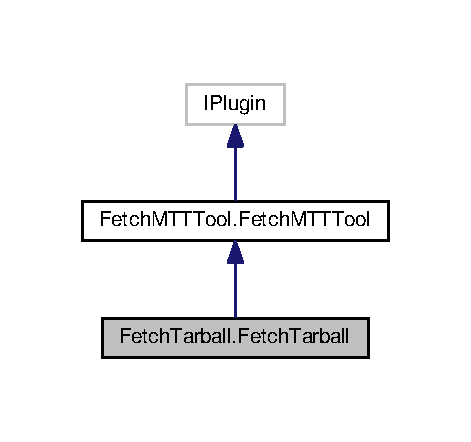
\includegraphics[width=226pt]{class_fetch_tarball_1_1_fetch_tarball__inherit__graph}
\end{center}
\end{figure}


Collaboration diagram for Fetch\-Tarball.\-Fetch\-Tarball\-:
\nopagebreak
\begin{figure}[H]
\begin{center}
\leavevmode
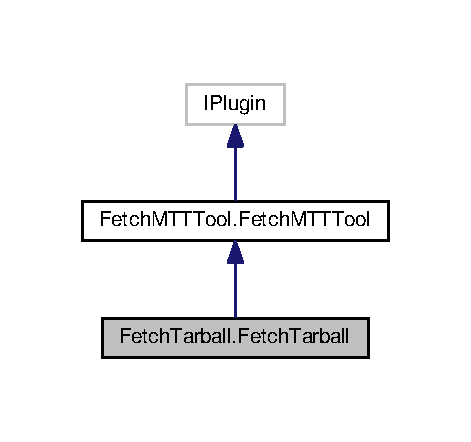
\includegraphics[width=226pt]{class_fetch_tarball_1_1_fetch_tarball__coll__graph}
\end{center}
\end{figure}
\subsection*{Public Member Functions}
\begin{DoxyCompactItemize}
\item 
def \hyperlink{class_fetch_tarball_1_1_fetch_tarball_a0fb0f6decddbd019212beb941b1d8b33}{\-\_\-\-\_\-init\-\_\-\-\_\-}
\item 
def \hyperlink{class_fetch_tarball_1_1_fetch_tarball_a9a88f8be0e5f6c54247c3a85da711f38}{activate}
\item 
def \hyperlink{class_fetch_tarball_1_1_fetch_tarball_aba185f1c1adad0aea744fc418093ffcf}{deactivate}
\item 
def \hyperlink{class_fetch_tarball_1_1_fetch_tarball_afcac4e7b528550c345ffca891b0f32fa}{print\-\_\-name}
\item 
def \hyperlink{class_fetch_tarball_1_1_fetch_tarball_a750d4f069ce00c62d8e44d1e5dd47d08}{print\-\_\-options}
\item 
def \hyperlink{class_fetch_tarball_1_1_fetch_tarball_ad99192c36d2f7200799fa8a2a37c6a5a}{execute}
\end{DoxyCompactItemize}
\subsection*{Public Attributes}
\begin{DoxyCompactItemize}
\item 
\hyperlink{class_fetch_tarball_1_1_fetch_tarball_a4e6818fd64191913c3f302485c2c4e96}{activated}
\item 
\hyperlink{class_fetch_tarball_1_1_fetch_tarball_ae733fd553804854c3beef59df1739732}{done}
\item 
\hyperlink{class_fetch_tarball_1_1_fetch_tarball_ae5c7611a1ef415c3e38c75ea803ef2e3}{options}
\end{DoxyCompactItemize}


\subsection{Detailed Description}


Definition at line 32 of file Fetch\-Tarball.\-py.



\subsection{Constructor \& Destructor Documentation}
\hypertarget{class_fetch_tarball_1_1_fetch_tarball_a0fb0f6decddbd019212beb941b1d8b33}{\index{Fetch\-Tarball\-::\-Fetch\-Tarball@{Fetch\-Tarball\-::\-Fetch\-Tarball}!\-\_\-\-\_\-init\-\_\-\-\_\-@{\-\_\-\-\_\-init\-\_\-\-\_\-}}
\index{\-\_\-\-\_\-init\-\_\-\-\_\-@{\-\_\-\-\_\-init\-\_\-\-\_\-}!FetchTarball::FetchTarball@{Fetch\-Tarball\-::\-Fetch\-Tarball}}
\subsubsection[{\-\_\-\-\_\-init\-\_\-\-\_\-}]{\setlength{\rightskip}{0pt plus 5cm}def Fetch\-Tarball.\-Fetch\-Tarball.\-\_\-\-\_\-init\-\_\-\-\_\- (
\begin{DoxyParamCaption}
\item[{}]{self}
\end{DoxyParamCaption}
)}}\label{class_fetch_tarball_1_1_fetch_tarball_a0fb0f6decddbd019212beb941b1d8b33}


Definition at line 34 of file Fetch\-Tarball.\-py.



\subsection{Member Function Documentation}
\hypertarget{class_fetch_tarball_1_1_fetch_tarball_a9a88f8be0e5f6c54247c3a85da711f38}{\index{Fetch\-Tarball\-::\-Fetch\-Tarball@{Fetch\-Tarball\-::\-Fetch\-Tarball}!activate@{activate}}
\index{activate@{activate}!FetchTarball::FetchTarball@{Fetch\-Tarball\-::\-Fetch\-Tarball}}
\subsubsection[{activate}]{\setlength{\rightskip}{0pt plus 5cm}def Fetch\-Tarball.\-Fetch\-Tarball.\-activate (
\begin{DoxyParamCaption}
\item[{}]{self}
\end{DoxyParamCaption}
)}}\label{class_fetch_tarball_1_1_fetch_tarball_a9a88f8be0e5f6c54247c3a85da711f38}


Definition at line 47 of file Fetch\-Tarball.\-py.

\hypertarget{class_fetch_tarball_1_1_fetch_tarball_aba185f1c1adad0aea744fc418093ffcf}{\index{Fetch\-Tarball\-::\-Fetch\-Tarball@{Fetch\-Tarball\-::\-Fetch\-Tarball}!deactivate@{deactivate}}
\index{deactivate@{deactivate}!FetchTarball::FetchTarball@{Fetch\-Tarball\-::\-Fetch\-Tarball}}
\subsubsection[{deactivate}]{\setlength{\rightskip}{0pt plus 5cm}def Fetch\-Tarball.\-Fetch\-Tarball.\-deactivate (
\begin{DoxyParamCaption}
\item[{}]{self}
\end{DoxyParamCaption}
)}}\label{class_fetch_tarball_1_1_fetch_tarball_aba185f1c1adad0aea744fc418093ffcf}


Definition at line 53 of file Fetch\-Tarball.\-py.

\hypertarget{class_fetch_tarball_1_1_fetch_tarball_ad99192c36d2f7200799fa8a2a37c6a5a}{\index{Fetch\-Tarball\-::\-Fetch\-Tarball@{Fetch\-Tarball\-::\-Fetch\-Tarball}!execute@{execute}}
\index{execute@{execute}!FetchTarball::FetchTarball@{Fetch\-Tarball\-::\-Fetch\-Tarball}}
\subsubsection[{execute}]{\setlength{\rightskip}{0pt plus 5cm}def Fetch\-Tarball.\-Fetch\-Tarball.\-execute (
\begin{DoxyParamCaption}
\item[{}]{self, }
\item[{}]{log, }
\item[{}]{keyvals, }
\item[{}]{test\-Def}
\end{DoxyParamCaption}
)}}\label{class_fetch_tarball_1_1_fetch_tarball_ad99192c36d2f7200799fa8a2a37c6a5a}


Definition at line 66 of file Fetch\-Tarball.\-py.

\hypertarget{class_fetch_tarball_1_1_fetch_tarball_afcac4e7b528550c345ffca891b0f32fa}{\index{Fetch\-Tarball\-::\-Fetch\-Tarball@{Fetch\-Tarball\-::\-Fetch\-Tarball}!print\-\_\-name@{print\-\_\-name}}
\index{print\-\_\-name@{print\-\_\-name}!FetchTarball::FetchTarball@{Fetch\-Tarball\-::\-Fetch\-Tarball}}
\subsubsection[{print\-\_\-name}]{\setlength{\rightskip}{0pt plus 5cm}def Fetch\-Tarball.\-Fetch\-Tarball.\-print\-\_\-name (
\begin{DoxyParamCaption}
\item[{}]{self}
\end{DoxyParamCaption}
)}}\label{class_fetch_tarball_1_1_fetch_tarball_afcac4e7b528550c345ffca891b0f32fa}


Definition at line 57 of file Fetch\-Tarball.\-py.

\hypertarget{class_fetch_tarball_1_1_fetch_tarball_a750d4f069ce00c62d8e44d1e5dd47d08}{\index{Fetch\-Tarball\-::\-Fetch\-Tarball@{Fetch\-Tarball\-::\-Fetch\-Tarball}!print\-\_\-options@{print\-\_\-options}}
\index{print\-\_\-options@{print\-\_\-options}!FetchTarball::FetchTarball@{Fetch\-Tarball\-::\-Fetch\-Tarball}}
\subsubsection[{print\-\_\-options}]{\setlength{\rightskip}{0pt plus 5cm}def Fetch\-Tarball.\-Fetch\-Tarball.\-print\-\_\-options (
\begin{DoxyParamCaption}
\item[{}]{self, }
\item[{}]{test\-Def, }
\item[{}]{prefix}
\end{DoxyParamCaption}
)}}\label{class_fetch_tarball_1_1_fetch_tarball_a750d4f069ce00c62d8e44d1e5dd47d08}


Definition at line 60 of file Fetch\-Tarball.\-py.



\subsection{Member Data Documentation}
\hypertarget{class_fetch_tarball_1_1_fetch_tarball_a4e6818fd64191913c3f302485c2c4e96}{\index{Fetch\-Tarball\-::\-Fetch\-Tarball@{Fetch\-Tarball\-::\-Fetch\-Tarball}!activated@{activated}}
\index{activated@{activated}!FetchTarball::FetchTarball@{Fetch\-Tarball\-::\-Fetch\-Tarball}}
\subsubsection[{activated}]{\setlength{\rightskip}{0pt plus 5cm}Fetch\-Tarball.\-Fetch\-Tarball.\-activated}}\label{class_fetch_tarball_1_1_fetch_tarball_a4e6818fd64191913c3f302485c2c4e96}


Definition at line 37 of file Fetch\-Tarball.\-py.

\hypertarget{class_fetch_tarball_1_1_fetch_tarball_ae733fd553804854c3beef59df1739732}{\index{Fetch\-Tarball\-::\-Fetch\-Tarball@{Fetch\-Tarball\-::\-Fetch\-Tarball}!done@{done}}
\index{done@{done}!FetchTarball::FetchTarball@{Fetch\-Tarball\-::\-Fetch\-Tarball}}
\subsubsection[{done}]{\setlength{\rightskip}{0pt plus 5cm}Fetch\-Tarball.\-Fetch\-Tarball.\-done}}\label{class_fetch_tarball_1_1_fetch_tarball_ae733fd553804854c3beef59df1739732}


Definition at line 40 of file Fetch\-Tarball.\-py.

\hypertarget{class_fetch_tarball_1_1_fetch_tarball_ae5c7611a1ef415c3e38c75ea803ef2e3}{\index{Fetch\-Tarball\-::\-Fetch\-Tarball@{Fetch\-Tarball\-::\-Fetch\-Tarball}!options@{options}}
\index{options@{options}!FetchTarball::FetchTarball@{Fetch\-Tarball\-::\-Fetch\-Tarball}}
\subsubsection[{options}]{\setlength{\rightskip}{0pt plus 5cm}Fetch\-Tarball.\-Fetch\-Tarball.\-options}}\label{class_fetch_tarball_1_1_fetch_tarball_ae5c7611a1ef415c3e38c75ea803ef2e3}


Definition at line 41 of file Fetch\-Tarball.\-py.



The documentation for this class was generated from the following file\-:\begin{DoxyCompactItemize}
\item 
/home/travis/build/open-\/mpi/mtt/pylib/\-Tools/\-Fetch/\hyperlink{_fetch_tarball_8py}{Fetch\-Tarball.\-py}\end{DoxyCompactItemize}

\input{class_firmware_m_t_t_stage_1_1_firmware_m_t_t_stage}
\input{class_foo_flash_1_1_foo_flash}
\hypertarget{class_git_1_1_git}{\section{Git.\-Git Class Reference}
\label{class_git_1_1_git}\index{Git.\-Git@{Git.\-Git}}
}


Inheritance diagram for Git.\-Git\-:
\nopagebreak
\begin{figure}[H]
\begin{center}
\leavevmode
\includegraphics[width=226pt]{class_git_1_1_git__inherit__graph}
\end{center}
\end{figure}


Collaboration diagram for Git.\-Git\-:
\nopagebreak
\begin{figure}[H]
\begin{center}
\leavevmode
\includegraphics[width=226pt]{class_git_1_1_git__coll__graph}
\end{center}
\end{figure}
\subsection*{Public Member Functions}
\begin{DoxyCompactItemize}
\item 
def \hyperlink{class_git_1_1_git_a19c57b8a20fad72c1090f8a07f6c00c0}{\-\_\-\-\_\-init\-\_\-\-\_\-}
\item 
def \hyperlink{class_git_1_1_git_a199ce28e3b17a99dd87b79b89bda524b}{activate}
\item 
def \hyperlink{class_git_1_1_git_a94824f2a863076683cf96a35bba71d46}{deactivate}
\item 
def \hyperlink{class_git_1_1_git_af7077c1aba1570b613f2f860504f668b}{print\-\_\-name}
\item 
def \hyperlink{class_git_1_1_git_a8f8145b83190e539ac8708f63a3e936b}{print\-\_\-options}
\item 
def \hyperlink{class_git_1_1_git_a6ae531f8f42d85850eda90f02bb184c3}{execute}
\end{DoxyCompactItemize}
\subsection*{Public Attributes}
\begin{DoxyCompactItemize}
\item 
\hyperlink{class_git_1_1_git_a22d3012cb93bad0a9122dd84afdfeee9}{activated}
\item 
\hyperlink{class_git_1_1_git_adb8991008d4bb4568fa9c2f991711cda}{done}
\item 
\hyperlink{class_git_1_1_git_a7560b88b014c5da8785739c7bb6283ed}{options}
\end{DoxyCompactItemize}


\subsection{Detailed Description}


Definition at line 36 of file Git.\-py.



\subsection{Constructor \& Destructor Documentation}
\hypertarget{class_git_1_1_git_a19c57b8a20fad72c1090f8a07f6c00c0}{\index{Git\-::\-Git@{Git\-::\-Git}!\-\_\-\-\_\-init\-\_\-\-\_\-@{\-\_\-\-\_\-init\-\_\-\-\_\-}}
\index{\-\_\-\-\_\-init\-\_\-\-\_\-@{\-\_\-\-\_\-init\-\_\-\-\_\-}!Git::Git@{Git\-::\-Git}}
\subsubsection[{\-\_\-\-\_\-init\-\_\-\-\_\-}]{\setlength{\rightskip}{0pt plus 5cm}def Git.\-Git.\-\_\-\-\_\-init\-\_\-\-\_\- (
\begin{DoxyParamCaption}
\item[{}]{self}
\end{DoxyParamCaption}
)}}\label{class_git_1_1_git_a19c57b8a20fad72c1090f8a07f6c00c0}


Definition at line 38 of file Git.\-py.



\subsection{Member Function Documentation}
\hypertarget{class_git_1_1_git_a199ce28e3b17a99dd87b79b89bda524b}{\index{Git\-::\-Git@{Git\-::\-Git}!activate@{activate}}
\index{activate@{activate}!Git::Git@{Git\-::\-Git}}
\subsubsection[{activate}]{\setlength{\rightskip}{0pt plus 5cm}def Git.\-Git.\-activate (
\begin{DoxyParamCaption}
\item[{}]{self}
\end{DoxyParamCaption}
)}}\label{class_git_1_1_git_a199ce28e3b17a99dd87b79b89bda524b}


Definition at line 59 of file Git.\-py.

\hypertarget{class_git_1_1_git_a94824f2a863076683cf96a35bba71d46}{\index{Git\-::\-Git@{Git\-::\-Git}!deactivate@{deactivate}}
\index{deactivate@{deactivate}!Git::Git@{Git\-::\-Git}}
\subsubsection[{deactivate}]{\setlength{\rightskip}{0pt plus 5cm}def Git.\-Git.\-deactivate (
\begin{DoxyParamCaption}
\item[{}]{self}
\end{DoxyParamCaption}
)}}\label{class_git_1_1_git_a94824f2a863076683cf96a35bba71d46}


Definition at line 65 of file Git.\-py.

\hypertarget{class_git_1_1_git_a6ae531f8f42d85850eda90f02bb184c3}{\index{Git\-::\-Git@{Git\-::\-Git}!execute@{execute}}
\index{execute@{execute}!Git::Git@{Git\-::\-Git}}
\subsubsection[{execute}]{\setlength{\rightskip}{0pt plus 5cm}def Git.\-Git.\-execute (
\begin{DoxyParamCaption}
\item[{}]{self, }
\item[{}]{log, }
\item[{}]{keyvals, }
\item[{}]{test\-Def}
\end{DoxyParamCaption}
)}}\label{class_git_1_1_git_a6ae531f8f42d85850eda90f02bb184c3}


Definition at line 78 of file Git.\-py.

\hypertarget{class_git_1_1_git_af7077c1aba1570b613f2f860504f668b}{\index{Git\-::\-Git@{Git\-::\-Git}!print\-\_\-name@{print\-\_\-name}}
\index{print\-\_\-name@{print\-\_\-name}!Git::Git@{Git\-::\-Git}}
\subsubsection[{print\-\_\-name}]{\setlength{\rightskip}{0pt plus 5cm}def Git.\-Git.\-print\-\_\-name (
\begin{DoxyParamCaption}
\item[{}]{self}
\end{DoxyParamCaption}
)}}\label{class_git_1_1_git_af7077c1aba1570b613f2f860504f668b}


Definition at line 69 of file Git.\-py.

\hypertarget{class_git_1_1_git_a8f8145b83190e539ac8708f63a3e936b}{\index{Git\-::\-Git@{Git\-::\-Git}!print\-\_\-options@{print\-\_\-options}}
\index{print\-\_\-options@{print\-\_\-options}!Git::Git@{Git\-::\-Git}}
\subsubsection[{print\-\_\-options}]{\setlength{\rightskip}{0pt plus 5cm}def Git.\-Git.\-print\-\_\-options (
\begin{DoxyParamCaption}
\item[{}]{self, }
\item[{}]{test\-Def, }
\item[{}]{prefix}
\end{DoxyParamCaption}
)}}\label{class_git_1_1_git_a8f8145b83190e539ac8708f63a3e936b}


Definition at line 72 of file Git.\-py.



\subsection{Member Data Documentation}
\hypertarget{class_git_1_1_git_a22d3012cb93bad0a9122dd84afdfeee9}{\index{Git\-::\-Git@{Git\-::\-Git}!activated@{activated}}
\index{activated@{activated}!Git::Git@{Git\-::\-Git}}
\subsubsection[{activated}]{\setlength{\rightskip}{0pt plus 5cm}Git.\-Git.\-activated}}\label{class_git_1_1_git_a22d3012cb93bad0a9122dd84afdfeee9}


Definition at line 41 of file Git.\-py.

\hypertarget{class_git_1_1_git_adb8991008d4bb4568fa9c2f991711cda}{\index{Git\-::\-Git@{Git\-::\-Git}!done@{done}}
\index{done@{done}!Git::Git@{Git\-::\-Git}}
\subsubsection[{done}]{\setlength{\rightskip}{0pt plus 5cm}Git.\-Git.\-done}}\label{class_git_1_1_git_adb8991008d4bb4568fa9c2f991711cda}


Definition at line 44 of file Git.\-py.

\hypertarget{class_git_1_1_git_a7560b88b014c5da8785739c7bb6283ed}{\index{Git\-::\-Git@{Git\-::\-Git}!options@{options}}
\index{options@{options}!Git::Git@{Git\-::\-Git}}
\subsubsection[{options}]{\setlength{\rightskip}{0pt plus 5cm}Git.\-Git.\-options}}\label{class_git_1_1_git_a7560b88b014c5da8785739c7bb6283ed}


Definition at line 45 of file Git.\-py.



The documentation for this class was generated from the following file\-:\begin{DoxyCompactItemize}
\item 
/home/travis/build/open-\/mpi/mtt/pylib/\-Tools/\-Fetch/\hyperlink{_git_8py}{Git.\-py}\end{DoxyCompactItemize}

\input{class_harasser_1_1_harasser}
\input{class_harasser_m_t_t_tool_1_1_harasser_m_t_t_tool}
\input{class_hostfile_1_1_hostfile}
\input{class_i_p_m_i_tool_1_1_i_p_m_i_tool}
\hypertarget{class_i_u_database_1_1_i_u_database}{\section{I\-U\-Database.\-I\-U\-Database Class Reference}
\label{class_i_u_database_1_1_i_u_database}\index{I\-U\-Database.\-I\-U\-Database@{I\-U\-Database.\-I\-U\-Database}}
}


Inheritance diagram for I\-U\-Database.\-I\-U\-Database\-:
\nopagebreak
\begin{figure}[H]
\begin{center}
\leavevmode
\includegraphics[width=220pt]{class_i_u_database_1_1_i_u_database__inherit__graph}
\end{center}
\end{figure}


Collaboration diagram for I\-U\-Database.\-I\-U\-Database\-:
\nopagebreak
\begin{figure}[H]
\begin{center}
\leavevmode
\includegraphics[width=220pt]{class_i_u_database_1_1_i_u_database__coll__graph}
\end{center}
\end{figure}
\subsection*{Public Member Functions}
\begin{DoxyCompactItemize}
\item 
def \hyperlink{class_i_u_database_1_1_i_u_database_aa12deecc4a4575f2f203e2bd1b8f0d59}{\-\_\-\-\_\-init\-\_\-\-\_\-}
\item 
def \hyperlink{class_i_u_database_1_1_i_u_database_ab53b555dbca9e121b4e5547f7ec2ecf5}{activate}
\item 
def \hyperlink{class_i_u_database_1_1_i_u_database_a57697e286ce6859233fbf07df5366b30}{deactivate}
\item 
def \hyperlink{class_i_u_database_1_1_i_u_database_a1c5472e3c083eda003ce17d0d40acbe3}{print\-\_\-name}
\item 
def \hyperlink{class_i_u_database_1_1_i_u_database_ac5175b773da96c0c792a262ad444c09c}{print\-\_\-options}
\item 
def \hyperlink{class_i_u_database_1_1_i_u_database_ab26ffba77df100f5b442fafa12e758ec}{execute}
\end{DoxyCompactItemize}
\subsection*{Public Attributes}
\begin{DoxyCompactItemize}
\item 
\hyperlink{class_i_u_database_1_1_i_u_database_a87c602469e1908c2c79859691839e9de}{options}
\item 
\hyperlink{class_i_u_database_1_1_i_u_database_a65d3fd103b54ba61830a606bd2258094}{cmds}
\end{DoxyCompactItemize}
\subsection*{Private Member Functions}
\begin{DoxyCompactItemize}
\item 
def \hyperlink{class_i_u_database_1_1_i_u_database_a98afecb796bd619142a3c440e9926d41}{\-\_\-merge\-\_\-dict}
\item 
def \hyperlink{class_i_u_database_1_1_i_u_database_a014e879e7f4eff72175443a886a8944f}{\-\_\-submit\-\_\-test\-\_\-run}
\item 
def \hyperlink{class_i_u_database_1_1_i_u_database_abfad8bfb6698d723b5cc99d303744c55}{\-\_\-submit\-\_\-test\-\_\-build}
\item 
def \hyperlink{class_i_u_database_1_1_i_u_database_a75e930a15c9ee4e1b7fa5dd4d5c4cfe9}{\-\_\-submit\-\_\-install}
\item 
def \hyperlink{class_i_u_database_1_1_i_u_database_abf478525045264145f74b84ff58adffc}{\-\_\-submit\-\_\-json\-\_\-data}
\item 
def \hyperlink{class_i_u_database_1_1_i_u_database_ad171afe463a3d8f70c2dc8ff92736bf0}{\-\_\-extract\-\_\-param}
\item 
def \hyperlink{class_i_u_database_1_1_i_u_database_a247089fa0f6a81a05e5a893de6503738}{\-\_\-get\-\_\-client\-\_\-serial}
\end{DoxyCompactItemize}


\subsection{Detailed Description}


Definition at line 47 of file I\-U\-Database.\-py.



\subsection{Constructor \& Destructor Documentation}
\hypertarget{class_i_u_database_1_1_i_u_database_aa12deecc4a4575f2f203e2bd1b8f0d59}{\index{I\-U\-Database\-::\-I\-U\-Database@{I\-U\-Database\-::\-I\-U\-Database}!\-\_\-\-\_\-init\-\_\-\-\_\-@{\-\_\-\-\_\-init\-\_\-\-\_\-}}
\index{\-\_\-\-\_\-init\-\_\-\-\_\-@{\-\_\-\-\_\-init\-\_\-\-\_\-}!IUDatabase::IUDatabase@{I\-U\-Database\-::\-I\-U\-Database}}
\subsubsection[{\-\_\-\-\_\-init\-\_\-\-\_\-}]{\setlength{\rightskip}{0pt plus 5cm}def I\-U\-Database.\-I\-U\-Database.\-\_\-\-\_\-init\-\_\-\-\_\- (
\begin{DoxyParamCaption}
\item[{}]{self}
\end{DoxyParamCaption}
)}}\label{class_i_u_database_1_1_i_u_database_aa12deecc4a4575f2f203e2bd1b8f0d59}


Definition at line 49 of file I\-U\-Database.\-py.



\subsection{Member Function Documentation}
\hypertarget{class_i_u_database_1_1_i_u_database_ad171afe463a3d8f70c2dc8ff92736bf0}{\index{I\-U\-Database\-::\-I\-U\-Database@{I\-U\-Database\-::\-I\-U\-Database}!\-\_\-extract\-\_\-param@{\-\_\-extract\-\_\-param}}
\index{\-\_\-extract\-\_\-param@{\-\_\-extract\-\_\-param}!IUDatabase::IUDatabase@{I\-U\-Database\-::\-I\-U\-Database}}
\subsubsection[{\-\_\-extract\-\_\-param}]{\setlength{\rightskip}{0pt plus 5cm}def I\-U\-Database.\-I\-U\-Database.\-\_\-extract\-\_\-param (
\begin{DoxyParamCaption}
\item[{}]{self, }
\item[{}]{logger, }
\item[{}]{section, }
\item[{}]{parameter}
\end{DoxyParamCaption}
)\hspace{0.3cm}{\ttfamily [private]}}}\label{class_i_u_database_1_1_i_u_database_ad171afe463a3d8f70c2dc8ff92736bf0}


Definition at line 895 of file I\-U\-Database.\-py.



Here is the caller graph for this function\-:
\nopagebreak
\begin{figure}[H]
\begin{center}
\leavevmode
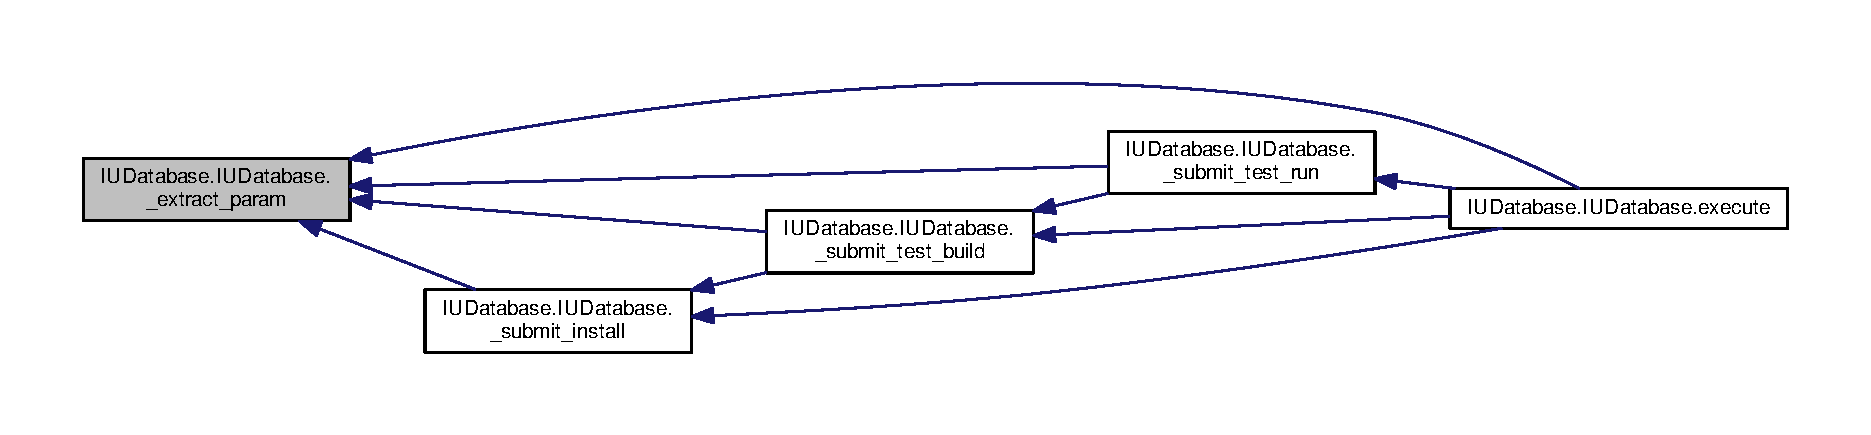
\includegraphics[width=350pt]{class_i_u_database_1_1_i_u_database_ad171afe463a3d8f70c2dc8ff92736bf0_icgraph}
\end{center}
\end{figure}


\hypertarget{class_i_u_database_1_1_i_u_database_a247089fa0f6a81a05e5a893de6503738}{\index{I\-U\-Database\-::\-I\-U\-Database@{I\-U\-Database\-::\-I\-U\-Database}!\-\_\-get\-\_\-client\-\_\-serial@{\-\_\-get\-\_\-client\-\_\-serial}}
\index{\-\_\-get\-\_\-client\-\_\-serial@{\-\_\-get\-\_\-client\-\_\-serial}!IUDatabase::IUDatabase@{I\-U\-Database\-::\-I\-U\-Database}}
\subsubsection[{\-\_\-get\-\_\-client\-\_\-serial}]{\setlength{\rightskip}{0pt plus 5cm}def I\-U\-Database.\-I\-U\-Database.\-\_\-get\-\_\-client\-\_\-serial (
\begin{DoxyParamCaption}
\item[{}]{self, }
\item[{}]{session, }
\item[{}]{url, }
\item[{}]{httpauth = {\ttfamily None}}
\end{DoxyParamCaption}
)\hspace{0.3cm}{\ttfamily [private]}}}\label{class_i_u_database_1_1_i_u_database_a247089fa0f6a81a05e5a893de6503738}


Definition at line 910 of file I\-U\-Database.\-py.



Here is the call graph for this function\-:
\nopagebreak
\begin{figure}[H]
\begin{center}
\leavevmode
\includegraphics[width=350pt]{class_i_u_database_1_1_i_u_database_a247089fa0f6a81a05e5a893de6503738_cgraph}
\end{center}
\end{figure}




Here is the caller graph for this function\-:
\nopagebreak
\begin{figure}[H]
\begin{center}
\leavevmode
\includegraphics[width=350pt]{class_i_u_database_1_1_i_u_database_a247089fa0f6a81a05e5a893de6503738_icgraph}
\end{center}
\end{figure}


\hypertarget{class_i_u_database_1_1_i_u_database_a98afecb796bd619142a3c440e9926d41}{\index{I\-U\-Database\-::\-I\-U\-Database@{I\-U\-Database\-::\-I\-U\-Database}!\-\_\-merge\-\_\-dict@{\-\_\-merge\-\_\-dict}}
\index{\-\_\-merge\-\_\-dict@{\-\_\-merge\-\_\-dict}!IUDatabase::IUDatabase@{I\-U\-Database\-::\-I\-U\-Database}}
\subsubsection[{\-\_\-merge\-\_\-dict}]{\setlength{\rightskip}{0pt plus 5cm}def I\-U\-Database.\-I\-U\-Database.\-\_\-merge\-\_\-dict (
\begin{DoxyParamCaption}
\item[{}]{self, }
\item[{}]{x, }
\item[{}]{y}
\end{DoxyParamCaption}
)\hspace{0.3cm}{\ttfamily [private]}}}\label{class_i_u_database_1_1_i_u_database_a98afecb796bd619142a3c440e9926d41}


Definition at line 225 of file I\-U\-Database.\-py.



Here is the caller graph for this function\-:
\nopagebreak
\begin{figure}[H]
\begin{center}
\leavevmode
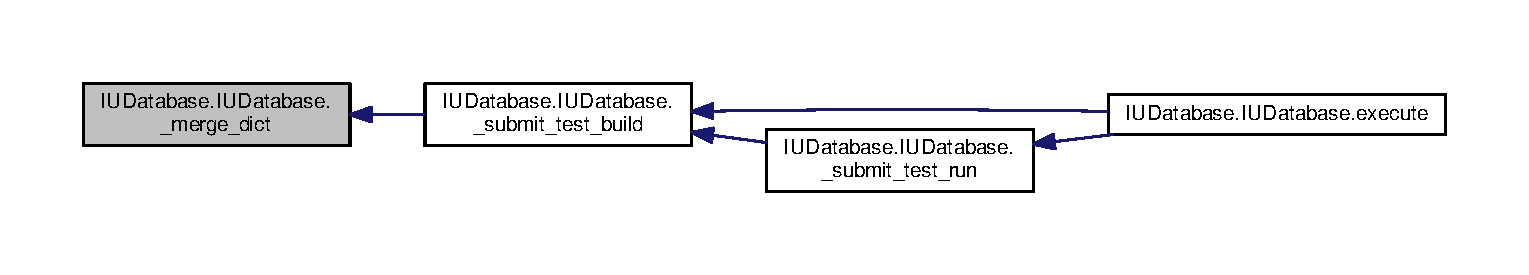
\includegraphics[width=350pt]{class_i_u_database_1_1_i_u_database_a98afecb796bd619142a3c440e9926d41_icgraph}
\end{center}
\end{figure}


\hypertarget{class_i_u_database_1_1_i_u_database_a75e930a15c9ee4e1b7fa5dd4d5c4cfe9}{\index{I\-U\-Database\-::\-I\-U\-Database@{I\-U\-Database\-::\-I\-U\-Database}!\-\_\-submit\-\_\-install@{\-\_\-submit\-\_\-install}}
\index{\-\_\-submit\-\_\-install@{\-\_\-submit\-\_\-install}!IUDatabase::IUDatabase@{I\-U\-Database\-::\-I\-U\-Database}}
\subsubsection[{\-\_\-submit\-\_\-install}]{\setlength{\rightskip}{0pt plus 5cm}def I\-U\-Database.\-I\-U\-Database.\-\_\-submit\-\_\-install (
\begin{DoxyParamCaption}
\item[{}]{self, }
\item[{}]{logger, }
\item[{}]{lg, }
\item[{}]{metadata, }
\item[{}]{s, }
\item[{}]{url, }
\item[{}]{httpauth = {\ttfamily None}}
\end{DoxyParamCaption}
)\hspace{0.3cm}{\ttfamily [private]}}}\label{class_i_u_database_1_1_i_u_database_a75e930a15c9ee4e1b7fa5dd4d5c4cfe9}


Definition at line 660 of file I\-U\-Database.\-py.



Here is the call graph for this function\-:
\nopagebreak
\begin{figure}[H]
\begin{center}
\leavevmode
\includegraphics[width=350pt]{class_i_u_database_1_1_i_u_database_a75e930a15c9ee4e1b7fa5dd4d5c4cfe9_cgraph}
\end{center}
\end{figure}




Here is the caller graph for this function\-:
\nopagebreak
\begin{figure}[H]
\begin{center}
\leavevmode
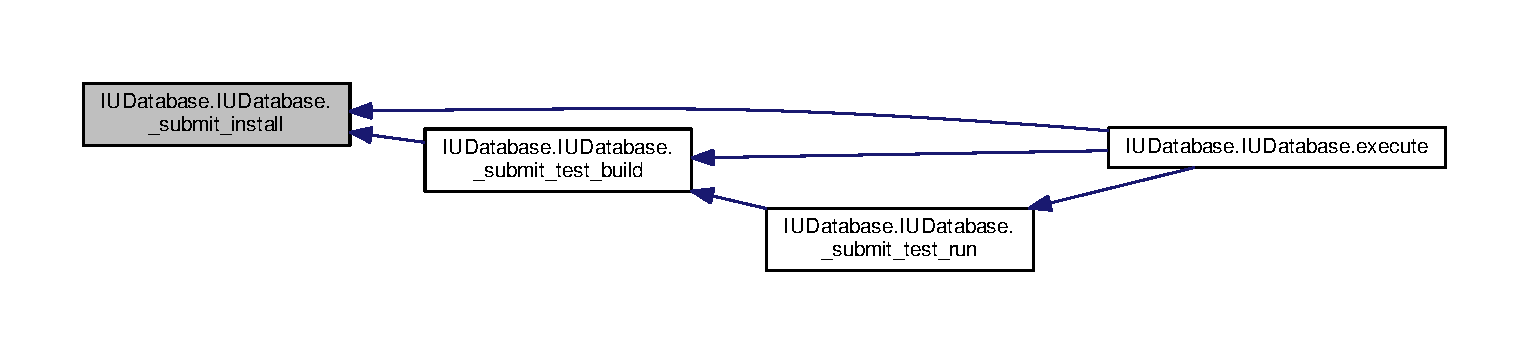
\includegraphics[width=350pt]{class_i_u_database_1_1_i_u_database_a75e930a15c9ee4e1b7fa5dd4d5c4cfe9_icgraph}
\end{center}
\end{figure}


\hypertarget{class_i_u_database_1_1_i_u_database_abf478525045264145f74b84ff58adffc}{\index{I\-U\-Database\-::\-I\-U\-Database@{I\-U\-Database\-::\-I\-U\-Database}!\-\_\-submit\-\_\-json\-\_\-data@{\-\_\-submit\-\_\-json\-\_\-data}}
\index{\-\_\-submit\-\_\-json\-\_\-data@{\-\_\-submit\-\_\-json\-\_\-data}!IUDatabase::IUDatabase@{I\-U\-Database\-::\-I\-U\-Database}}
\subsubsection[{\-\_\-submit\-\_\-json\-\_\-data}]{\setlength{\rightskip}{0pt plus 5cm}def I\-U\-Database.\-I\-U\-Database.\-\_\-submit\-\_\-json\-\_\-data (
\begin{DoxyParamCaption}
\item[{}]{self, }
\item[{}]{payload, }
\item[{}]{s, }
\item[{}]{url, }
\item[{}]{httpauth = {\ttfamily None}}
\end{DoxyParamCaption}
)\hspace{0.3cm}{\ttfamily [private]}}}\label{class_i_u_database_1_1_i_u_database_abf478525045264145f74b84ff58adffc}


Definition at line 858 of file I\-U\-Database.\-py.



Here is the caller graph for this function\-:
\nopagebreak
\begin{figure}[H]
\begin{center}
\leavevmode
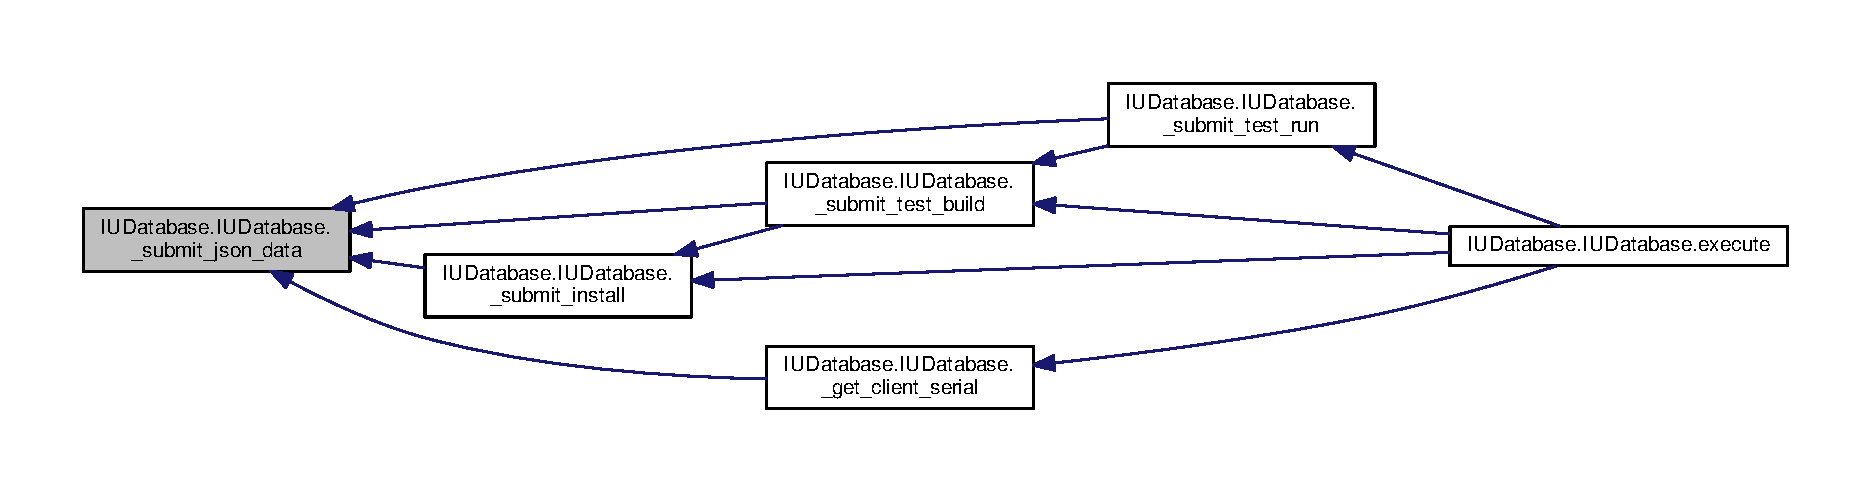
\includegraphics[width=350pt]{class_i_u_database_1_1_i_u_database_abf478525045264145f74b84ff58adffc_icgraph}
\end{center}
\end{figure}


\hypertarget{class_i_u_database_1_1_i_u_database_abfad8bfb6698d723b5cc99d303744c55}{\index{I\-U\-Database\-::\-I\-U\-Database@{I\-U\-Database\-::\-I\-U\-Database}!\-\_\-submit\-\_\-test\-\_\-build@{\-\_\-submit\-\_\-test\-\_\-build}}
\index{\-\_\-submit\-\_\-test\-\_\-build@{\-\_\-submit\-\_\-test\-\_\-build}!IUDatabase::IUDatabase@{I\-U\-Database\-::\-I\-U\-Database}}
\subsubsection[{\-\_\-submit\-\_\-test\-\_\-build}]{\setlength{\rightskip}{0pt plus 5cm}def I\-U\-Database.\-I\-U\-Database.\-\_\-submit\-\_\-test\-\_\-build (
\begin{DoxyParamCaption}
\item[{}]{self, }
\item[{}]{logger, }
\item[{}]{lg, }
\item[{}]{metadata, }
\item[{}]{s, }
\item[{}]{url, }
\item[{}]{httpauth = {\ttfamily None}}
\end{DoxyParamCaption}
)\hspace{0.3cm}{\ttfamily [private]}}}\label{class_i_u_database_1_1_i_u_database_abfad8bfb6698d723b5cc99d303744c55}


Definition at line 502 of file I\-U\-Database.\-py.



Here is the call graph for this function\-:
\nopagebreak
\begin{figure}[H]
\begin{center}
\leavevmode
\includegraphics[width=350pt]{class_i_u_database_1_1_i_u_database_abfad8bfb6698d723b5cc99d303744c55_cgraph}
\end{center}
\end{figure}




Here is the caller graph for this function\-:
\nopagebreak
\begin{figure}[H]
\begin{center}
\leavevmode
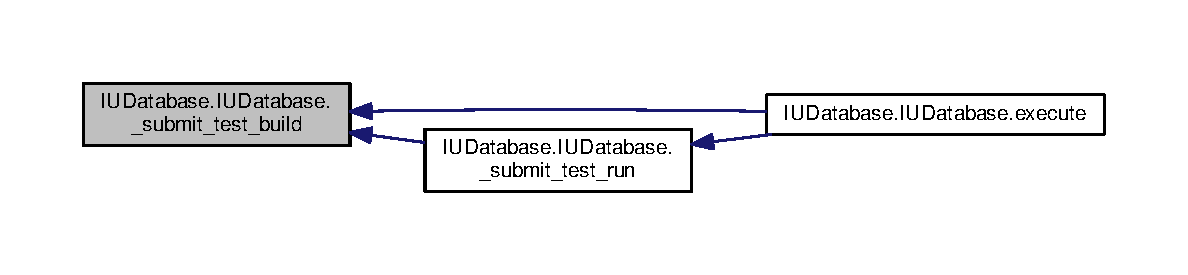
\includegraphics[width=350pt]{class_i_u_database_1_1_i_u_database_abfad8bfb6698d723b5cc99d303744c55_icgraph}
\end{center}
\end{figure}


\hypertarget{class_i_u_database_1_1_i_u_database_a014e879e7f4eff72175443a886a8944f}{\index{I\-U\-Database\-::\-I\-U\-Database@{I\-U\-Database\-::\-I\-U\-Database}!\-\_\-submit\-\_\-test\-\_\-run@{\-\_\-submit\-\_\-test\-\_\-run}}
\index{\-\_\-submit\-\_\-test\-\_\-run@{\-\_\-submit\-\_\-test\-\_\-run}!IUDatabase::IUDatabase@{I\-U\-Database\-::\-I\-U\-Database}}
\subsubsection[{\-\_\-submit\-\_\-test\-\_\-run}]{\setlength{\rightskip}{0pt plus 5cm}def I\-U\-Database.\-I\-U\-Database.\-\_\-submit\-\_\-test\-\_\-run (
\begin{DoxyParamCaption}
\item[{}]{self, }
\item[{}]{logger, }
\item[{}]{lg, }
\item[{}]{metadata, }
\item[{}]{s, }
\item[{}]{url, }
\item[{}]{test\-Def, }
\item[{}]{httpauth = {\ttfamily None}}
\end{DoxyParamCaption}
)\hspace{0.3cm}{\ttfamily [private]}}}\label{class_i_u_database_1_1_i_u_database_a014e879e7f4eff72175443a886a8944f}


Definition at line 230 of file I\-U\-Database.\-py.



Here is the call graph for this function\-:
\nopagebreak
\begin{figure}[H]
\begin{center}
\leavevmode
\includegraphics[width=350pt]{class_i_u_database_1_1_i_u_database_a014e879e7f4eff72175443a886a8944f_cgraph}
\end{center}
\end{figure}




Here is the caller graph for this function\-:
\nopagebreak
\begin{figure}[H]
\begin{center}
\leavevmode
\includegraphics[width=350pt]{class_i_u_database_1_1_i_u_database_a014e879e7f4eff72175443a886a8944f_icgraph}
\end{center}
\end{figure}


\hypertarget{class_i_u_database_1_1_i_u_database_ab53b555dbca9e121b4e5547f7ec2ecf5}{\index{I\-U\-Database\-::\-I\-U\-Database@{I\-U\-Database\-::\-I\-U\-Database}!activate@{activate}}
\index{activate@{activate}!IUDatabase::IUDatabase@{I\-U\-Database\-::\-I\-U\-Database}}
\subsubsection[{activate}]{\setlength{\rightskip}{0pt plus 5cm}def I\-U\-Database.\-I\-U\-Database.\-activate (
\begin{DoxyParamCaption}
\item[{}]{self}
\end{DoxyParamCaption}
)}}\label{class_i_u_database_1_1_i_u_database_ab53b555dbca9e121b4e5547f7ec2ecf5}


Definition at line 68 of file I\-U\-Database.\-py.

\hypertarget{class_i_u_database_1_1_i_u_database_a57697e286ce6859233fbf07df5366b30}{\index{I\-U\-Database\-::\-I\-U\-Database@{I\-U\-Database\-::\-I\-U\-Database}!deactivate@{deactivate}}
\index{deactivate@{deactivate}!IUDatabase::IUDatabase@{I\-U\-Database\-::\-I\-U\-Database}}
\subsubsection[{deactivate}]{\setlength{\rightskip}{0pt plus 5cm}def I\-U\-Database.\-I\-U\-Database.\-deactivate (
\begin{DoxyParamCaption}
\item[{}]{self}
\end{DoxyParamCaption}
)}}\label{class_i_u_database_1_1_i_u_database_a57697e286ce6859233fbf07df5366b30}


Definition at line 74 of file I\-U\-Database.\-py.

\hypertarget{class_i_u_database_1_1_i_u_database_ab26ffba77df100f5b442fafa12e758ec}{\index{I\-U\-Database\-::\-I\-U\-Database@{I\-U\-Database\-::\-I\-U\-Database}!execute@{execute}}
\index{execute@{execute}!IUDatabase::IUDatabase@{I\-U\-Database\-::\-I\-U\-Database}}
\subsubsection[{execute}]{\setlength{\rightskip}{0pt plus 5cm}def I\-U\-Database.\-I\-U\-Database.\-execute (
\begin{DoxyParamCaption}
\item[{}]{self, }
\item[{}]{log, }
\item[{}]{keyvals, }
\item[{}]{test\-Def}
\end{DoxyParamCaption}
)}}\label{class_i_u_database_1_1_i_u_database_ab26ffba77df100f5b442fafa12e758ec}


Definition at line 87 of file I\-U\-Database.\-py.



Here is the call graph for this function\-:
\nopagebreak
\begin{figure}[H]
\begin{center}
\leavevmode
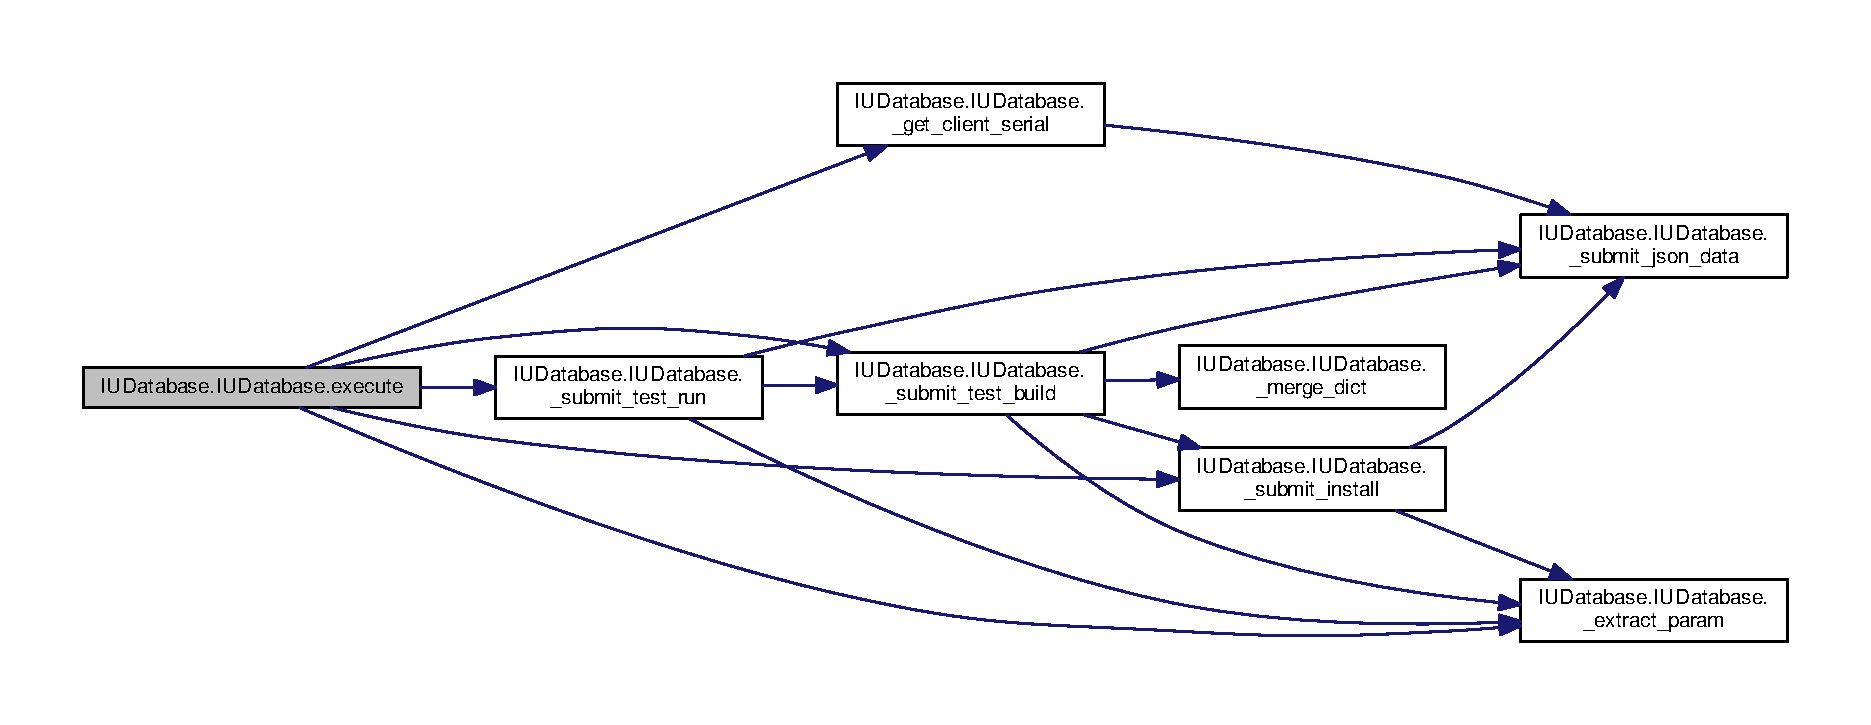
\includegraphics[width=350pt]{class_i_u_database_1_1_i_u_database_ab26ffba77df100f5b442fafa12e758ec_cgraph}
\end{center}
\end{figure}


\hypertarget{class_i_u_database_1_1_i_u_database_a1c5472e3c083eda003ce17d0d40acbe3}{\index{I\-U\-Database\-::\-I\-U\-Database@{I\-U\-Database\-::\-I\-U\-Database}!print\-\_\-name@{print\-\_\-name}}
\index{print\-\_\-name@{print\-\_\-name}!IUDatabase::IUDatabase@{I\-U\-Database\-::\-I\-U\-Database}}
\subsubsection[{print\-\_\-name}]{\setlength{\rightskip}{0pt plus 5cm}def I\-U\-Database.\-I\-U\-Database.\-print\-\_\-name (
\begin{DoxyParamCaption}
\item[{}]{self}
\end{DoxyParamCaption}
)}}\label{class_i_u_database_1_1_i_u_database_a1c5472e3c083eda003ce17d0d40acbe3}


Definition at line 78 of file I\-U\-Database.\-py.

\hypertarget{class_i_u_database_1_1_i_u_database_ac5175b773da96c0c792a262ad444c09c}{\index{I\-U\-Database\-::\-I\-U\-Database@{I\-U\-Database\-::\-I\-U\-Database}!print\-\_\-options@{print\-\_\-options}}
\index{print\-\_\-options@{print\-\_\-options}!IUDatabase::IUDatabase@{I\-U\-Database\-::\-I\-U\-Database}}
\subsubsection[{print\-\_\-options}]{\setlength{\rightskip}{0pt plus 5cm}def I\-U\-Database.\-I\-U\-Database.\-print\-\_\-options (
\begin{DoxyParamCaption}
\item[{}]{self, }
\item[{}]{test\-Def, }
\item[{}]{prefix}
\end{DoxyParamCaption}
)}}\label{class_i_u_database_1_1_i_u_database_ac5175b773da96c0c792a262ad444c09c}


Definition at line 81 of file I\-U\-Database.\-py.



\subsection{Member Data Documentation}
\hypertarget{class_i_u_database_1_1_i_u_database_a65d3fd103b54ba61830a606bd2258094}{\index{I\-U\-Database\-::\-I\-U\-Database@{I\-U\-Database\-::\-I\-U\-Database}!cmds@{cmds}}
\index{cmds@{cmds}!IUDatabase::IUDatabase@{I\-U\-Database\-::\-I\-U\-Database}}
\subsubsection[{cmds}]{\setlength{\rightskip}{0pt plus 5cm}I\-U\-Database.\-I\-U\-Database.\-cmds}}\label{class_i_u_database_1_1_i_u_database_a65d3fd103b54ba61830a606bd2258094}


Definition at line 66 of file I\-U\-Database.\-py.

\hypertarget{class_i_u_database_1_1_i_u_database_a87c602469e1908c2c79859691839e9de}{\index{I\-U\-Database\-::\-I\-U\-Database@{I\-U\-Database\-::\-I\-U\-Database}!options@{options}}
\index{options@{options}!IUDatabase::IUDatabase@{I\-U\-Database\-::\-I\-U\-Database}}
\subsubsection[{options}]{\setlength{\rightskip}{0pt plus 5cm}I\-U\-Database.\-I\-U\-Database.\-options}}\label{class_i_u_database_1_1_i_u_database_a87c602469e1908c2c79859691839e9de}


Definition at line 52 of file I\-U\-Database.\-py.



The documentation for this class was generated from the following file\-:\begin{DoxyCompactItemize}
\item 
/home/travis/build/open-\/mpi/mtt/pylib/\-Stages/\-Reporter/\hyperlink{_i_u_database_8py}{I\-U\-Database.\-py}\end{DoxyCompactItemize}

\input{class_junit_x_m_l_1_1_junit_x_m_l}
\hypertarget{class_execute_cmd_1_1_kill_process_thread}{\section{Execute\-Cmd.\-Kill\-Process\-Thread Class Reference}
\label{class_execute_cmd_1_1_kill_process_thread}\index{Execute\-Cmd.\-Kill\-Process\-Thread@{Execute\-Cmd.\-Kill\-Process\-Thread}}
}


Inheritance diagram for Execute\-Cmd.\-Kill\-Process\-Thread\-:
\nopagebreak
\begin{figure}[H]
\begin{center}
\leavevmode
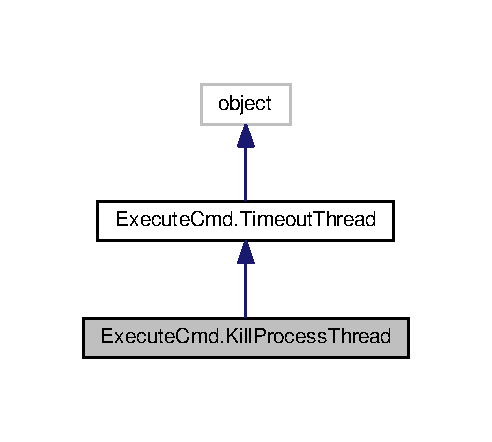
\includegraphics[width=236pt]{class_execute_cmd_1_1_kill_process_thread__inherit__graph}
\end{center}
\end{figure}


Collaboration diagram for Execute\-Cmd.\-Kill\-Process\-Thread\-:
\nopagebreak
\begin{figure}[H]
\begin{center}
\leavevmode
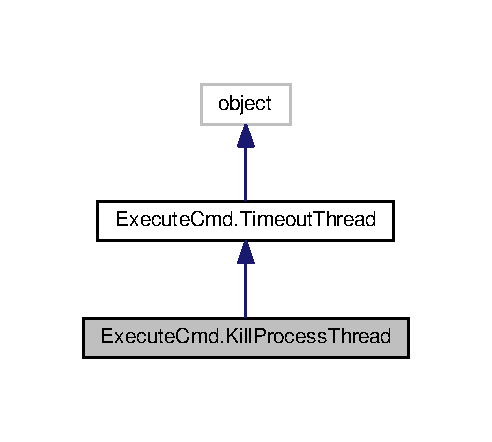
\includegraphics[width=236pt]{class_execute_cmd_1_1_kill_process_thread__coll__graph}
\end{center}
\end{figure}
\subsection*{Public Member Functions}
\begin{DoxyCompactItemize}
\item 
def \hyperlink{class_execute_cmd_1_1_kill_process_thread_a414bcd0a32109602bf07fb94ed69bef3}{\-\_\-\-\_\-init\-\_\-\-\_\-}
\item 
def \hyperlink{class_execute_cmd_1_1_kill_process_thread_a19365e409f39f61d0eb67d0769bd829c}{timed\-\_\-out}
\end{DoxyCompactItemize}
\subsection*{Public Attributes}
\begin{DoxyCompactItemize}
\item 
\hyperlink{class_execute_cmd_1_1_kill_process_thread_a66ec3fdeb7fad04cd760e3ede0903e65}{pid}
\end{DoxyCompactItemize}


\subsection{Detailed Description}


Definition at line 53 of file Execute\-Cmd.\-py.



\subsection{Constructor \& Destructor Documentation}
\hypertarget{class_execute_cmd_1_1_kill_process_thread_a414bcd0a32109602bf07fb94ed69bef3}{\index{Execute\-Cmd\-::\-Kill\-Process\-Thread@{Execute\-Cmd\-::\-Kill\-Process\-Thread}!\-\_\-\-\_\-init\-\_\-\-\_\-@{\-\_\-\-\_\-init\-\_\-\-\_\-}}
\index{\-\_\-\-\_\-init\-\_\-\-\_\-@{\-\_\-\-\_\-init\-\_\-\-\_\-}!ExecuteCmd::KillProcessThread@{Execute\-Cmd\-::\-Kill\-Process\-Thread}}
\subsubsection[{\-\_\-\-\_\-init\-\_\-\-\_\-}]{\setlength{\rightskip}{0pt plus 5cm}def Execute\-Cmd.\-Kill\-Process\-Thread.\-\_\-\-\_\-init\-\_\-\-\_\- (
\begin{DoxyParamCaption}
\item[{}]{self, }
\item[{}]{seconds, }
\item[{}]{pid}
\end{DoxyParamCaption}
)}}\label{class_execute_cmd_1_1_kill_process_thread_a414bcd0a32109602bf07fb94ed69bef3}


Definition at line 54 of file Execute\-Cmd.\-py.



\subsection{Member Function Documentation}
\hypertarget{class_execute_cmd_1_1_kill_process_thread_a19365e409f39f61d0eb67d0769bd829c}{\index{Execute\-Cmd\-::\-Kill\-Process\-Thread@{Execute\-Cmd\-::\-Kill\-Process\-Thread}!timed\-\_\-out@{timed\-\_\-out}}
\index{timed\-\_\-out@{timed\-\_\-out}!ExecuteCmd::KillProcessThread@{Execute\-Cmd\-::\-Kill\-Process\-Thread}}
\subsubsection[{timed\-\_\-out}]{\setlength{\rightskip}{0pt plus 5cm}def Execute\-Cmd.\-Kill\-Process\-Thread.\-timed\-\_\-out (
\begin{DoxyParamCaption}
\item[{}]{self}
\end{DoxyParamCaption}
)}}\label{class_execute_cmd_1_1_kill_process_thread_a19365e409f39f61d0eb67d0769bd829c}


Definition at line 58 of file Execute\-Cmd.\-py.



\subsection{Member Data Documentation}
\hypertarget{class_execute_cmd_1_1_kill_process_thread_a66ec3fdeb7fad04cd760e3ede0903e65}{\index{Execute\-Cmd\-::\-Kill\-Process\-Thread@{Execute\-Cmd\-::\-Kill\-Process\-Thread}!pid@{pid}}
\index{pid@{pid}!ExecuteCmd::KillProcessThread@{Execute\-Cmd\-::\-Kill\-Process\-Thread}}
\subsubsection[{pid}]{\setlength{\rightskip}{0pt plus 5cm}Execute\-Cmd.\-Kill\-Process\-Thread.\-pid}}\label{class_execute_cmd_1_1_kill_process_thread_a66ec3fdeb7fad04cd760e3ede0903e65}


Definition at line 56 of file Execute\-Cmd.\-py.



The documentation for this class was generated from the following file\-:\begin{DoxyCompactItemize}
\item 
/home/travis/build/open-\/mpi/mtt/pylib/\-Utilities/\hyperlink{_execute_cmd_8py}{Execute\-Cmd.\-py}\end{DoxyCompactItemize}

\input{class_launcher_defaults_m_t_t_stage_1_1_launcher_defaults_m_t_t_stage}
\hypertarget{class_launcher_m_t_t_tool_1_1_launcher_m_t_t_tool}{\section{Launcher\-M\-T\-T\-Tool.\-Launcher\-M\-T\-T\-Tool Class Reference}
\label{class_launcher_m_t_t_tool_1_1_launcher_m_t_t_tool}\index{Launcher\-M\-T\-T\-Tool.\-Launcher\-M\-T\-T\-Tool@{Launcher\-M\-T\-T\-Tool.\-Launcher\-M\-T\-T\-Tool}}
}


Inheritance diagram for Launcher\-M\-T\-T\-Tool.\-Launcher\-M\-T\-T\-Tool\-:
\nopagebreak
\begin{figure}[H]
\begin{center}
\leavevmode
\includegraphics[width=350pt]{class_launcher_m_t_t_tool_1_1_launcher_m_t_t_tool__inherit__graph}
\end{center}
\end{figure}


Collaboration diagram for Launcher\-M\-T\-T\-Tool.\-Launcher\-M\-T\-T\-Tool\-:
\nopagebreak
\begin{figure}[H]
\begin{center}
\leavevmode
\includegraphics[width=218pt]{class_launcher_m_t_t_tool_1_1_launcher_m_t_t_tool__coll__graph}
\end{center}
\end{figure}
\subsection*{Public Member Functions}
\begin{DoxyCompactItemize}
\item 
def \hyperlink{class_launcher_m_t_t_tool_1_1_launcher_m_t_t_tool_acfc089fc18fcde378ce794b64211d537}{\-\_\-\-\_\-init\-\_\-\-\_\-}
\item 
def \hyperlink{class_launcher_m_t_t_tool_1_1_launcher_m_t_t_tool_a07b353aff1a7768e40b46e67e47c9c21}{print\-\_\-name}
\item 
def \hyperlink{class_launcher_m_t_t_tool_1_1_launcher_m_t_t_tool_a40c4c403d5553eb13f91e91e8dc973f6}{update\-Defaults}
\item 
def \hyperlink{class_launcher_m_t_t_tool_1_1_launcher_m_t_t_tool_a0a3d37e54fc308a806e95816143059f5}{setup\-Paths}
\item 
def \hyperlink{class_launcher_m_t_t_tool_1_1_launcher_m_t_t_tool_a95b352e21a72a37e29645ab632a8fe5e}{reset\-Paths}
\item 
def \hyperlink{class_launcher_m_t_t_tool_1_1_launcher_m_t_t_tool_a3cd99128c246981fedf691483e21b79d}{collect\-Tests}
\item 
def \hyperlink{class_launcher_m_t_t_tool_1_1_launcher_m_t_t_tool_a60e6315e0652c6787600a1669e22e3a0}{allocate\-Cluster}
\item 
def \hyperlink{class_launcher_m_t_t_tool_1_1_launcher_m_t_t_tool_aed1deaa222bb1908e29562f51aadf65f}{run\-Tests}
\item 
def \hyperlink{class_launcher_m_t_t_tool_1_1_launcher_m_t_t_tool_ae446b720803ee6ba3ab9febc001573dd}{deallocate\-Cluster}
\end{DoxyCompactItemize}
\subsection*{Public Attributes}
\begin{DoxyCompactItemize}
\item 
\hyperlink{class_launcher_m_t_t_tool_1_1_launcher_m_t_t_tool_a2810a82208a2846540adffee0a6855f7}{tests}
\item 
\hyperlink{class_launcher_m_t_t_tool_1_1_launcher_m_t_t_tool_a03696ab743c22417d3be183903c20a68}{skip\-\_\-tests}
\item 
\hyperlink{class_launcher_m_t_t_tool_1_1_launcher_m_t_t_tool_acf34764e2b173537cbf5720cc0a1235d}{oldbinpath}
\item 
\hyperlink{class_launcher_m_t_t_tool_1_1_launcher_m_t_t_tool_abb2e78c53544b045ef3ab42ed8b68806}{oldldlibpath}
\item 
\hyperlink{class_launcher_m_t_t_tool_1_1_launcher_m_t_t_tool_a4d5ba97c121703a52364ba25f4a2546b}{skip\-Status}
\item 
\hyperlink{class_launcher_m_t_t_tool_1_1_launcher_m_t_t_tool_ae68abb344ae827a5ce0ee79446020c63}{expected\-\_\-returncodes}
\item 
\hyperlink{class_launcher_m_t_t_tool_1_1_launcher_m_t_t_tool_a24a3038f22807231f60be1efd39f7bcb}{final\-Status}
\item 
\hyperlink{class_launcher_m_t_t_tool_1_1_launcher_m_t_t_tool_a607ea8851059a23f64f5b1ef4590109e}{final\-Error}
\item 
\hyperlink{class_launcher_m_t_t_tool_1_1_launcher_m_t_t_tool_a397beae73724893629842d0031c64526}{num\-Tests}
\item 
\hyperlink{class_launcher_m_t_t_tool_1_1_launcher_m_t_t_tool_a92a3dc1fd9b7d2e9129d3a0968a871eb}{num\-Pass}
\item 
\hyperlink{class_launcher_m_t_t_tool_1_1_launcher_m_t_t_tool_affd7de54ccbc2c7f78b4afa06728f5e5}{num\-Skip}
\item 
\hyperlink{class_launcher_m_t_t_tool_1_1_launcher_m_t_t_tool_a17fe6e6f8981cc1f7cd1953cac37668a}{num\-Fail}
\item 
\hyperlink{class_launcher_m_t_t_tool_1_1_launcher_m_t_t_tool_ae2be62c3d068b4c1c3d7c1ddaf4cfdbe}{num\-Timed}
\item 
\hyperlink{class_launcher_m_t_t_tool_1_1_launcher_m_t_t_tool_aa8e59ca462ace6b189cd849a08afa639}{max\-Tests}
\item 
\hyperlink{class_launcher_m_t_t_tool_1_1_launcher_m_t_t_tool_a37f255feb0dac2f1eb0e6eff2746bd7b}{midpath}
\item 
\hyperlink{class_launcher_m_t_t_tool_1_1_launcher_m_t_t_tool_a13b93dfdaa7c433967c808d9bf54dcf9}{location}
\item 
\hyperlink{class_launcher_m_t_t_tool_1_1_launcher_m_t_t_tool_a7bcf1056b03f3777ef4ed39f7e063f36}{cwd}
\item 
\hyperlink{class_launcher_m_t_t_tool_1_1_launcher_m_t_t_tool_a79266b94da58ec136cca44c1f735d3a7}{allocated}
\end{DoxyCompactItemize}


\subsection{Detailed Description}


Definition at line 25 of file Launcher\-M\-T\-T\-Tool.\-py.



\subsection{Constructor \& Destructor Documentation}
\hypertarget{class_launcher_m_t_t_tool_1_1_launcher_m_t_t_tool_acfc089fc18fcde378ce794b64211d537}{\index{Launcher\-M\-T\-T\-Tool\-::\-Launcher\-M\-T\-T\-Tool@{Launcher\-M\-T\-T\-Tool\-::\-Launcher\-M\-T\-T\-Tool}!\-\_\-\-\_\-init\-\_\-\-\_\-@{\-\_\-\-\_\-init\-\_\-\-\_\-}}
\index{\-\_\-\-\_\-init\-\_\-\-\_\-@{\-\_\-\-\_\-init\-\_\-\-\_\-}!LauncherMTTTool::LauncherMTTTool@{Launcher\-M\-T\-T\-Tool\-::\-Launcher\-M\-T\-T\-Tool}}
\subsubsection[{\-\_\-\-\_\-init\-\_\-\-\_\-}]{\setlength{\rightskip}{0pt plus 5cm}def Launcher\-M\-T\-T\-Tool.\-Launcher\-M\-T\-T\-Tool.\-\_\-\-\_\-init\-\_\-\-\_\- (
\begin{DoxyParamCaption}
\item[{}]{self}
\end{DoxyParamCaption}
)}}\label{class_launcher_m_t_t_tool_1_1_launcher_m_t_t_tool_acfc089fc18fcde378ce794b64211d537}


Definition at line 26 of file Launcher\-M\-T\-T\-Tool.\-py.



\subsection{Member Function Documentation}
\hypertarget{class_launcher_m_t_t_tool_1_1_launcher_m_t_t_tool_a60e6315e0652c6787600a1669e22e3a0}{\index{Launcher\-M\-T\-T\-Tool\-::\-Launcher\-M\-T\-T\-Tool@{Launcher\-M\-T\-T\-Tool\-::\-Launcher\-M\-T\-T\-Tool}!allocate\-Cluster@{allocate\-Cluster}}
\index{allocate\-Cluster@{allocate\-Cluster}!LauncherMTTTool::LauncherMTTTool@{Launcher\-M\-T\-T\-Tool\-::\-Launcher\-M\-T\-T\-Tool}}
\subsubsection[{allocate\-Cluster}]{\setlength{\rightskip}{0pt plus 5cm}def Launcher\-M\-T\-T\-Tool.\-Launcher\-M\-T\-T\-Tool.\-allocate\-Cluster (
\begin{DoxyParamCaption}
\item[{}]{self, }
\item[{}]{log, }
\item[{}]{cmds, }
\item[{}]{test\-Def}
\end{DoxyParamCaption}
)}}\label{class_launcher_m_t_t_tool_1_1_launcher_m_t_t_tool_a60e6315e0652c6787600a1669e22e3a0}


Definition at line 358 of file Launcher\-M\-T\-T\-Tool.\-py.



Here is the caller graph for this function\-:
\nopagebreak
\begin{figure}[H]
\begin{center}
\leavevmode
\includegraphics[width=350pt]{class_launcher_m_t_t_tool_1_1_launcher_m_t_t_tool_a60e6315e0652c6787600a1669e22e3a0_icgraph}
\end{center}
\end{figure}


\hypertarget{class_launcher_m_t_t_tool_1_1_launcher_m_t_t_tool_a3cd99128c246981fedf691483e21b79d}{\index{Launcher\-M\-T\-T\-Tool\-::\-Launcher\-M\-T\-T\-Tool@{Launcher\-M\-T\-T\-Tool\-::\-Launcher\-M\-T\-T\-Tool}!collect\-Tests@{collect\-Tests}}
\index{collect\-Tests@{collect\-Tests}!LauncherMTTTool::LauncherMTTTool@{Launcher\-M\-T\-T\-Tool\-::\-Launcher\-M\-T\-T\-Tool}}
\subsubsection[{collect\-Tests}]{\setlength{\rightskip}{0pt plus 5cm}def Launcher\-M\-T\-T\-Tool.\-Launcher\-M\-T\-T\-Tool.\-collect\-Tests (
\begin{DoxyParamCaption}
\item[{}]{self, }
\item[{}]{log, }
\item[{}]{cmds}
\end{DoxyParamCaption}
)}}\label{class_launcher_m_t_t_tool_1_1_launcher_m_t_t_tool_a3cd99128c246981fedf691483e21b79d}


Definition at line 219 of file Launcher\-M\-T\-T\-Tool.\-py.



Here is the caller graph for this function\-:
\nopagebreak
\begin{figure}[H]
\begin{center}
\leavevmode
\includegraphics[width=350pt]{class_launcher_m_t_t_tool_1_1_launcher_m_t_t_tool_a3cd99128c246981fedf691483e21b79d_icgraph}
\end{center}
\end{figure}


\hypertarget{class_launcher_m_t_t_tool_1_1_launcher_m_t_t_tool_ae446b720803ee6ba3ab9febc001573dd}{\index{Launcher\-M\-T\-T\-Tool\-::\-Launcher\-M\-T\-T\-Tool@{Launcher\-M\-T\-T\-Tool\-::\-Launcher\-M\-T\-T\-Tool}!deallocate\-Cluster@{deallocate\-Cluster}}
\index{deallocate\-Cluster@{deallocate\-Cluster}!LauncherMTTTool::LauncherMTTTool@{Launcher\-M\-T\-T\-Tool\-::\-Launcher\-M\-T\-T\-Tool}}
\subsubsection[{deallocate\-Cluster}]{\setlength{\rightskip}{0pt plus 5cm}def Launcher\-M\-T\-T\-Tool.\-Launcher\-M\-T\-T\-Tool.\-deallocate\-Cluster (
\begin{DoxyParamCaption}
\item[{}]{self, }
\item[{}]{log, }
\item[{}]{cmds, }
\item[{}]{test\-Def}
\end{DoxyParamCaption}
)}}\label{class_launcher_m_t_t_tool_1_1_launcher_m_t_t_tool_ae446b720803ee6ba3ab9febc001573dd}


Definition at line 491 of file Launcher\-M\-T\-T\-Tool.\-py.



Here is the caller graph for this function\-:
\nopagebreak
\begin{figure}[H]
\begin{center}
\leavevmode
\includegraphics[width=350pt]{class_launcher_m_t_t_tool_1_1_launcher_m_t_t_tool_ae446b720803ee6ba3ab9febc001573dd_icgraph}
\end{center}
\end{figure}


\hypertarget{class_launcher_m_t_t_tool_1_1_launcher_m_t_t_tool_a07b353aff1a7768e40b46e67e47c9c21}{\index{Launcher\-M\-T\-T\-Tool\-::\-Launcher\-M\-T\-T\-Tool@{Launcher\-M\-T\-T\-Tool\-::\-Launcher\-M\-T\-T\-Tool}!print\-\_\-name@{print\-\_\-name}}
\index{print\-\_\-name@{print\-\_\-name}!LauncherMTTTool::LauncherMTTTool@{Launcher\-M\-T\-T\-Tool\-::\-Launcher\-M\-T\-T\-Tool}}
\subsubsection[{print\-\_\-name}]{\setlength{\rightskip}{0pt plus 5cm}def Launcher\-M\-T\-T\-Tool.\-Launcher\-M\-T\-T\-Tool.\-print\-\_\-name (
\begin{DoxyParamCaption}
\item[{}]{self}
\end{DoxyParamCaption}
)}}\label{class_launcher_m_t_t_tool_1_1_launcher_m_t_t_tool_a07b353aff1a7768e40b46e67e47c9c21}


Definition at line 45 of file Launcher\-M\-T\-T\-Tool.\-py.

\hypertarget{class_launcher_m_t_t_tool_1_1_launcher_m_t_t_tool_a95b352e21a72a37e29645ab632a8fe5e}{\index{Launcher\-M\-T\-T\-Tool\-::\-Launcher\-M\-T\-T\-Tool@{Launcher\-M\-T\-T\-Tool\-::\-Launcher\-M\-T\-T\-Tool}!reset\-Paths@{reset\-Paths}}
\index{reset\-Paths@{reset\-Paths}!LauncherMTTTool::LauncherMTTTool@{Launcher\-M\-T\-T\-Tool\-::\-Launcher\-M\-T\-T\-Tool}}
\subsubsection[{reset\-Paths}]{\setlength{\rightskip}{0pt plus 5cm}def Launcher\-M\-T\-T\-Tool.\-Launcher\-M\-T\-T\-Tool.\-reset\-Paths (
\begin{DoxyParamCaption}
\item[{}]{self, }
\item[{}]{log, }
\item[{}]{test\-Def}
\end{DoxyParamCaption}
)}}\label{class_launcher_m_t_t_tool_1_1_launcher_m_t_t_tool_a95b352e21a72a37e29645ab632a8fe5e}


Definition at line 202 of file Launcher\-M\-T\-T\-Tool.\-py.



Here is the caller graph for this function\-:
\nopagebreak
\begin{figure}[H]
\begin{center}
\leavevmode
\includegraphics[width=350pt]{class_launcher_m_t_t_tool_1_1_launcher_m_t_t_tool_a95b352e21a72a37e29645ab632a8fe5e_icgraph}
\end{center}
\end{figure}


\hypertarget{class_launcher_m_t_t_tool_1_1_launcher_m_t_t_tool_aed1deaa222bb1908e29562f51aadf65f}{\index{Launcher\-M\-T\-T\-Tool\-::\-Launcher\-M\-T\-T\-Tool@{Launcher\-M\-T\-T\-Tool\-::\-Launcher\-M\-T\-T\-Tool}!run\-Tests@{run\-Tests}}
\index{run\-Tests@{run\-Tests}!LauncherMTTTool::LauncherMTTTool@{Launcher\-M\-T\-T\-Tool\-::\-Launcher\-M\-T\-T\-Tool}}
\subsubsection[{run\-Tests}]{\setlength{\rightskip}{0pt plus 5cm}def Launcher\-M\-T\-T\-Tool.\-Launcher\-M\-T\-T\-Tool.\-run\-Tests (
\begin{DoxyParamCaption}
\item[{}]{self, }
\item[{}]{log, }
\item[{}]{cmdargs, }
\item[{}]{cmds, }
\item[{}]{test\-Def}
\end{DoxyParamCaption}
)}}\label{class_launcher_m_t_t_tool_1_1_launcher_m_t_t_tool_aed1deaa222bb1908e29562f51aadf65f}


Definition at line 371 of file Launcher\-M\-T\-T\-Tool.\-py.



Here is the caller graph for this function\-:
\nopagebreak
\begin{figure}[H]
\begin{center}
\leavevmode
\includegraphics[width=350pt]{class_launcher_m_t_t_tool_1_1_launcher_m_t_t_tool_aed1deaa222bb1908e29562f51aadf65f_icgraph}
\end{center}
\end{figure}


\hypertarget{class_launcher_m_t_t_tool_1_1_launcher_m_t_t_tool_a0a3d37e54fc308a806e95816143059f5}{\index{Launcher\-M\-T\-T\-Tool\-::\-Launcher\-M\-T\-T\-Tool@{Launcher\-M\-T\-T\-Tool\-::\-Launcher\-M\-T\-T\-Tool}!setup\-Paths@{setup\-Paths}}
\index{setup\-Paths@{setup\-Paths}!LauncherMTTTool::LauncherMTTTool@{Launcher\-M\-T\-T\-Tool\-::\-Launcher\-M\-T\-T\-Tool}}
\subsubsection[{setup\-Paths}]{\setlength{\rightskip}{0pt plus 5cm}def Launcher\-M\-T\-T\-Tool.\-Launcher\-M\-T\-T\-Tool.\-setup\-Paths (
\begin{DoxyParamCaption}
\item[{}]{self, }
\item[{}]{log, }
\item[{}]{keyvals, }
\item[{}]{cmds, }
\item[{}]{test\-Def}
\end{DoxyParamCaption}
)}}\label{class_launcher_m_t_t_tool_1_1_launcher_m_t_t_tool_a0a3d37e54fc308a806e95816143059f5}


Definition at line 78 of file Launcher\-M\-T\-T\-Tool.\-py.



Here is the caller graph for this function\-:
\nopagebreak
\begin{figure}[H]
\begin{center}
\leavevmode
\includegraphics[width=350pt]{class_launcher_m_t_t_tool_1_1_launcher_m_t_t_tool_a0a3d37e54fc308a806e95816143059f5_icgraph}
\end{center}
\end{figure}


\hypertarget{class_launcher_m_t_t_tool_1_1_launcher_m_t_t_tool_a40c4c403d5553eb13f91e91e8dc973f6}{\index{Launcher\-M\-T\-T\-Tool\-::\-Launcher\-M\-T\-T\-Tool@{Launcher\-M\-T\-T\-Tool\-::\-Launcher\-M\-T\-T\-Tool}!update\-Defaults@{update\-Defaults}}
\index{update\-Defaults@{update\-Defaults}!LauncherMTTTool::LauncherMTTTool@{Launcher\-M\-T\-T\-Tool\-::\-Launcher\-M\-T\-T\-Tool}}
\subsubsection[{update\-Defaults}]{\setlength{\rightskip}{0pt plus 5cm}def Launcher\-M\-T\-T\-Tool.\-Launcher\-M\-T\-T\-Tool.\-update\-Defaults (
\begin{DoxyParamCaption}
\item[{}]{self, }
\item[{}]{log, }
\item[{}]{options, }
\item[{}]{keyvals, }
\item[{}]{test\-Def}
\end{DoxyParamCaption}
)}}\label{class_launcher_m_t_t_tool_1_1_launcher_m_t_t_tool_a40c4c403d5553eb13f91e91e8dc973f6}


Definition at line 48 of file Launcher\-M\-T\-T\-Tool.\-py.



Here is the caller graph for this function\-:
\nopagebreak
\begin{figure}[H]
\begin{center}
\leavevmode
\includegraphics[width=350pt]{class_launcher_m_t_t_tool_1_1_launcher_m_t_t_tool_a40c4c403d5553eb13f91e91e8dc973f6_icgraph}
\end{center}
\end{figure}




\subsection{Member Data Documentation}
\hypertarget{class_launcher_m_t_t_tool_1_1_launcher_m_t_t_tool_a79266b94da58ec136cca44c1f735d3a7}{\index{Launcher\-M\-T\-T\-Tool\-::\-Launcher\-M\-T\-T\-Tool@{Launcher\-M\-T\-T\-Tool\-::\-Launcher\-M\-T\-T\-Tool}!allocated@{allocated}}
\index{allocated@{allocated}!LauncherMTTTool::LauncherMTTTool@{Launcher\-M\-T\-T\-Tool\-::\-Launcher\-M\-T\-T\-Tool}}
\subsubsection[{allocated}]{\setlength{\rightskip}{0pt plus 5cm}Launcher\-M\-T\-T\-Tool.\-Launcher\-M\-T\-T\-Tool.\-allocated}}\label{class_launcher_m_t_t_tool_1_1_launcher_m_t_t_tool_a79266b94da58ec136cca44c1f735d3a7}


Definition at line 359 of file Launcher\-M\-T\-T\-Tool.\-py.

\hypertarget{class_launcher_m_t_t_tool_1_1_launcher_m_t_t_tool_a7bcf1056b03f3777ef4ed39f7e063f36}{\index{Launcher\-M\-T\-T\-Tool\-::\-Launcher\-M\-T\-T\-Tool@{Launcher\-M\-T\-T\-Tool\-::\-Launcher\-M\-T\-T\-Tool}!cwd@{cwd}}
\index{cwd@{cwd}!LauncherMTTTool::LauncherMTTTool@{Launcher\-M\-T\-T\-Tool\-::\-Launcher\-M\-T\-T\-Tool}}
\subsubsection[{cwd}]{\setlength{\rightskip}{0pt plus 5cm}Launcher\-M\-T\-T\-Tool.\-Launcher\-M\-T\-T\-Tool.\-cwd}}\label{class_launcher_m_t_t_tool_1_1_launcher_m_t_t_tool_a7bcf1056b03f3777ef4ed39f7e063f36}


Definition at line 196 of file Launcher\-M\-T\-T\-Tool.\-py.

\hypertarget{class_launcher_m_t_t_tool_1_1_launcher_m_t_t_tool_ae68abb344ae827a5ce0ee79446020c63}{\index{Launcher\-M\-T\-T\-Tool\-::\-Launcher\-M\-T\-T\-Tool@{Launcher\-M\-T\-T\-Tool\-::\-Launcher\-M\-T\-T\-Tool}!expected\-\_\-returncodes@{expected\-\_\-returncodes}}
\index{expected\-\_\-returncodes@{expected\-\_\-returncodes}!LauncherMTTTool::LauncherMTTTool@{Launcher\-M\-T\-T\-Tool\-::\-Launcher\-M\-T\-T\-Tool}}
\subsubsection[{expected\-\_\-returncodes}]{\setlength{\rightskip}{0pt plus 5cm}Launcher\-M\-T\-T\-Tool.\-Launcher\-M\-T\-T\-Tool.\-expected\-\_\-returncodes}}\label{class_launcher_m_t_t_tool_1_1_launcher_m_t_t_tool_ae68abb344ae827a5ce0ee79446020c63}


Definition at line 32 of file Launcher\-M\-T\-T\-Tool.\-py.

\hypertarget{class_launcher_m_t_t_tool_1_1_launcher_m_t_t_tool_a607ea8851059a23f64f5b1ef4590109e}{\index{Launcher\-M\-T\-T\-Tool\-::\-Launcher\-M\-T\-T\-Tool@{Launcher\-M\-T\-T\-Tool\-::\-Launcher\-M\-T\-T\-Tool}!final\-Error@{final\-Error}}
\index{final\-Error@{final\-Error}!LauncherMTTTool::LauncherMTTTool@{Launcher\-M\-T\-T\-Tool\-::\-Launcher\-M\-T\-T\-Tool}}
\subsubsection[{final\-Error}]{\setlength{\rightskip}{0pt plus 5cm}Launcher\-M\-T\-T\-Tool.\-Launcher\-M\-T\-T\-Tool.\-final\-Error}}\label{class_launcher_m_t_t_tool_1_1_launcher_m_t_t_tool_a607ea8851059a23f64f5b1ef4590109e}


Definition at line 34 of file Launcher\-M\-T\-T\-Tool.\-py.

\hypertarget{class_launcher_m_t_t_tool_1_1_launcher_m_t_t_tool_a24a3038f22807231f60be1efd39f7bcb}{\index{Launcher\-M\-T\-T\-Tool\-::\-Launcher\-M\-T\-T\-Tool@{Launcher\-M\-T\-T\-Tool\-::\-Launcher\-M\-T\-T\-Tool}!final\-Status@{final\-Status}}
\index{final\-Status@{final\-Status}!LauncherMTTTool::LauncherMTTTool@{Launcher\-M\-T\-T\-Tool\-::\-Launcher\-M\-T\-T\-Tool}}
\subsubsection[{final\-Status}]{\setlength{\rightskip}{0pt plus 5cm}Launcher\-M\-T\-T\-Tool.\-Launcher\-M\-T\-T\-Tool.\-final\-Status}}\label{class_launcher_m_t_t_tool_1_1_launcher_m_t_t_tool_a24a3038f22807231f60be1efd39f7bcb}


Definition at line 33 of file Launcher\-M\-T\-T\-Tool.\-py.

\hypertarget{class_launcher_m_t_t_tool_1_1_launcher_m_t_t_tool_a13b93dfdaa7c433967c808d9bf54dcf9}{\index{Launcher\-M\-T\-T\-Tool\-::\-Launcher\-M\-T\-T\-Tool@{Launcher\-M\-T\-T\-Tool\-::\-Launcher\-M\-T\-T\-Tool}!location@{location}}
\index{location@{location}!LauncherMTTTool::LauncherMTTTool@{Launcher\-M\-T\-T\-Tool\-::\-Launcher\-M\-T\-T\-Tool}}
\subsubsection[{location}]{\setlength{\rightskip}{0pt plus 5cm}Launcher\-M\-T\-T\-Tool.\-Launcher\-M\-T\-T\-Tool.\-location}}\label{class_launcher_m_t_t_tool_1_1_launcher_m_t_t_tool_a13b93dfdaa7c433967c808d9bf54dcf9}


Definition at line 87 of file Launcher\-M\-T\-T\-Tool.\-py.

\hypertarget{class_launcher_m_t_t_tool_1_1_launcher_m_t_t_tool_aa8e59ca462ace6b189cd849a08afa639}{\index{Launcher\-M\-T\-T\-Tool\-::\-Launcher\-M\-T\-T\-Tool@{Launcher\-M\-T\-T\-Tool\-::\-Launcher\-M\-T\-T\-Tool}!max\-Tests@{max\-Tests}}
\index{max\-Tests@{max\-Tests}!LauncherMTTTool::LauncherMTTTool@{Launcher\-M\-T\-T\-Tool\-::\-Launcher\-M\-T\-T\-Tool}}
\subsubsection[{max\-Tests}]{\setlength{\rightskip}{0pt plus 5cm}Launcher\-M\-T\-T\-Tool.\-Launcher\-M\-T\-T\-Tool.\-max\-Tests}}\label{class_launcher_m_t_t_tool_1_1_launcher_m_t_t_tool_aa8e59ca462ace6b189cd849a08afa639}


Definition at line 40 of file Launcher\-M\-T\-T\-Tool.\-py.

\hypertarget{class_launcher_m_t_t_tool_1_1_launcher_m_t_t_tool_a37f255feb0dac2f1eb0e6eff2746bd7b}{\index{Launcher\-M\-T\-T\-Tool\-::\-Launcher\-M\-T\-T\-Tool@{Launcher\-M\-T\-T\-Tool\-::\-Launcher\-M\-T\-T\-Tool}!midpath@{midpath}}
\index{midpath@{midpath}!LauncherMTTTool::LauncherMTTTool@{Launcher\-M\-T\-T\-Tool\-::\-Launcher\-M\-T\-T\-Tool}}
\subsubsection[{midpath}]{\setlength{\rightskip}{0pt plus 5cm}Launcher\-M\-T\-T\-Tool.\-Launcher\-M\-T\-T\-Tool.\-midpath}}\label{class_launcher_m_t_t_tool_1_1_launcher_m_t_t_tool_a37f255feb0dac2f1eb0e6eff2746bd7b}


Definition at line 41 of file Launcher\-M\-T\-T\-Tool.\-py.

\hypertarget{class_launcher_m_t_t_tool_1_1_launcher_m_t_t_tool_a17fe6e6f8981cc1f7cd1953cac37668a}{\index{Launcher\-M\-T\-T\-Tool\-::\-Launcher\-M\-T\-T\-Tool@{Launcher\-M\-T\-T\-Tool\-::\-Launcher\-M\-T\-T\-Tool}!num\-Fail@{num\-Fail}}
\index{num\-Fail@{num\-Fail}!LauncherMTTTool::LauncherMTTTool@{Launcher\-M\-T\-T\-Tool\-::\-Launcher\-M\-T\-T\-Tool}}
\subsubsection[{num\-Fail}]{\setlength{\rightskip}{0pt plus 5cm}Launcher\-M\-T\-T\-Tool.\-Launcher\-M\-T\-T\-Tool.\-num\-Fail}}\label{class_launcher_m_t_t_tool_1_1_launcher_m_t_t_tool_a17fe6e6f8981cc1f7cd1953cac37668a}


Definition at line 38 of file Launcher\-M\-T\-T\-Tool.\-py.

\hypertarget{class_launcher_m_t_t_tool_1_1_launcher_m_t_t_tool_a92a3dc1fd9b7d2e9129d3a0968a871eb}{\index{Launcher\-M\-T\-T\-Tool\-::\-Launcher\-M\-T\-T\-Tool@{Launcher\-M\-T\-T\-Tool\-::\-Launcher\-M\-T\-T\-Tool}!num\-Pass@{num\-Pass}}
\index{num\-Pass@{num\-Pass}!LauncherMTTTool::LauncherMTTTool@{Launcher\-M\-T\-T\-Tool\-::\-Launcher\-M\-T\-T\-Tool}}
\subsubsection[{num\-Pass}]{\setlength{\rightskip}{0pt plus 5cm}Launcher\-M\-T\-T\-Tool.\-Launcher\-M\-T\-T\-Tool.\-num\-Pass}}\label{class_launcher_m_t_t_tool_1_1_launcher_m_t_t_tool_a92a3dc1fd9b7d2e9129d3a0968a871eb}


Definition at line 36 of file Launcher\-M\-T\-T\-Tool.\-py.

\hypertarget{class_launcher_m_t_t_tool_1_1_launcher_m_t_t_tool_affd7de54ccbc2c7f78b4afa06728f5e5}{\index{Launcher\-M\-T\-T\-Tool\-::\-Launcher\-M\-T\-T\-Tool@{Launcher\-M\-T\-T\-Tool\-::\-Launcher\-M\-T\-T\-Tool}!num\-Skip@{num\-Skip}}
\index{num\-Skip@{num\-Skip}!LauncherMTTTool::LauncherMTTTool@{Launcher\-M\-T\-T\-Tool\-::\-Launcher\-M\-T\-T\-Tool}}
\subsubsection[{num\-Skip}]{\setlength{\rightskip}{0pt plus 5cm}Launcher\-M\-T\-T\-Tool.\-Launcher\-M\-T\-T\-Tool.\-num\-Skip}}\label{class_launcher_m_t_t_tool_1_1_launcher_m_t_t_tool_affd7de54ccbc2c7f78b4afa06728f5e5}


Definition at line 37 of file Launcher\-M\-T\-T\-Tool.\-py.

\hypertarget{class_launcher_m_t_t_tool_1_1_launcher_m_t_t_tool_a397beae73724893629842d0031c64526}{\index{Launcher\-M\-T\-T\-Tool\-::\-Launcher\-M\-T\-T\-Tool@{Launcher\-M\-T\-T\-Tool\-::\-Launcher\-M\-T\-T\-Tool}!num\-Tests@{num\-Tests}}
\index{num\-Tests@{num\-Tests}!LauncherMTTTool::LauncherMTTTool@{Launcher\-M\-T\-T\-Tool\-::\-Launcher\-M\-T\-T\-Tool}}
\subsubsection[{num\-Tests}]{\setlength{\rightskip}{0pt plus 5cm}Launcher\-M\-T\-T\-Tool.\-Launcher\-M\-T\-T\-Tool.\-num\-Tests}}\label{class_launcher_m_t_t_tool_1_1_launcher_m_t_t_tool_a397beae73724893629842d0031c64526}


Definition at line 35 of file Launcher\-M\-T\-T\-Tool.\-py.

\hypertarget{class_launcher_m_t_t_tool_1_1_launcher_m_t_t_tool_ae2be62c3d068b4c1c3d7c1ddaf4cfdbe}{\index{Launcher\-M\-T\-T\-Tool\-::\-Launcher\-M\-T\-T\-Tool@{Launcher\-M\-T\-T\-Tool\-::\-Launcher\-M\-T\-T\-Tool}!num\-Timed@{num\-Timed}}
\index{num\-Timed@{num\-Timed}!LauncherMTTTool::LauncherMTTTool@{Launcher\-M\-T\-T\-Tool\-::\-Launcher\-M\-T\-T\-Tool}}
\subsubsection[{num\-Timed}]{\setlength{\rightskip}{0pt plus 5cm}Launcher\-M\-T\-T\-Tool.\-Launcher\-M\-T\-T\-Tool.\-num\-Timed}}\label{class_launcher_m_t_t_tool_1_1_launcher_m_t_t_tool_ae2be62c3d068b4c1c3d7c1ddaf4cfdbe}


Definition at line 39 of file Launcher\-M\-T\-T\-Tool.\-py.

\hypertarget{class_launcher_m_t_t_tool_1_1_launcher_m_t_t_tool_acf34764e2b173537cbf5720cc0a1235d}{\index{Launcher\-M\-T\-T\-Tool\-::\-Launcher\-M\-T\-T\-Tool@{Launcher\-M\-T\-T\-Tool\-::\-Launcher\-M\-T\-T\-Tool}!oldbinpath@{oldbinpath}}
\index{oldbinpath@{oldbinpath}!LauncherMTTTool::LauncherMTTTool@{Launcher\-M\-T\-T\-Tool\-::\-Launcher\-M\-T\-T\-Tool}}
\subsubsection[{oldbinpath}]{\setlength{\rightskip}{0pt plus 5cm}Launcher\-M\-T\-T\-Tool.\-Launcher\-M\-T\-T\-Tool.\-oldbinpath}}\label{class_launcher_m_t_t_tool_1_1_launcher_m_t_t_tool_acf34764e2b173537cbf5720cc0a1235d}


Definition at line 29 of file Launcher\-M\-T\-T\-Tool.\-py.

\hypertarget{class_launcher_m_t_t_tool_1_1_launcher_m_t_t_tool_abb2e78c53544b045ef3ab42ed8b68806}{\index{Launcher\-M\-T\-T\-Tool\-::\-Launcher\-M\-T\-T\-Tool@{Launcher\-M\-T\-T\-Tool\-::\-Launcher\-M\-T\-T\-Tool}!oldldlibpath@{oldldlibpath}}
\index{oldldlibpath@{oldldlibpath}!LauncherMTTTool::LauncherMTTTool@{Launcher\-M\-T\-T\-Tool\-::\-Launcher\-M\-T\-T\-Tool}}
\subsubsection[{oldldlibpath}]{\setlength{\rightskip}{0pt plus 5cm}Launcher\-M\-T\-T\-Tool.\-Launcher\-M\-T\-T\-Tool.\-oldldlibpath}}\label{class_launcher_m_t_t_tool_1_1_launcher_m_t_t_tool_abb2e78c53544b045ef3ab42ed8b68806}


Definition at line 30 of file Launcher\-M\-T\-T\-Tool.\-py.

\hypertarget{class_launcher_m_t_t_tool_1_1_launcher_m_t_t_tool_a03696ab743c22417d3be183903c20a68}{\index{Launcher\-M\-T\-T\-Tool\-::\-Launcher\-M\-T\-T\-Tool@{Launcher\-M\-T\-T\-Tool\-::\-Launcher\-M\-T\-T\-Tool}!skip\-\_\-tests@{skip\-\_\-tests}}
\index{skip\-\_\-tests@{skip\-\_\-tests}!LauncherMTTTool::LauncherMTTTool@{Launcher\-M\-T\-T\-Tool\-::\-Launcher\-M\-T\-T\-Tool}}
\subsubsection[{skip\-\_\-tests}]{\setlength{\rightskip}{0pt plus 5cm}Launcher\-M\-T\-T\-Tool.\-Launcher\-M\-T\-T\-Tool.\-skip\-\_\-tests}}\label{class_launcher_m_t_t_tool_1_1_launcher_m_t_t_tool_a03696ab743c22417d3be183903c20a68}


Definition at line 28 of file Launcher\-M\-T\-T\-Tool.\-py.

\hypertarget{class_launcher_m_t_t_tool_1_1_launcher_m_t_t_tool_a4d5ba97c121703a52364ba25f4a2546b}{\index{Launcher\-M\-T\-T\-Tool\-::\-Launcher\-M\-T\-T\-Tool@{Launcher\-M\-T\-T\-Tool\-::\-Launcher\-M\-T\-T\-Tool}!skip\-Status@{skip\-Status}}
\index{skip\-Status@{skip\-Status}!LauncherMTTTool::LauncherMTTTool@{Launcher\-M\-T\-T\-Tool\-::\-Launcher\-M\-T\-T\-Tool}}
\subsubsection[{skip\-Status}]{\setlength{\rightskip}{0pt plus 5cm}Launcher\-M\-T\-T\-Tool.\-Launcher\-M\-T\-T\-Tool.\-skip\-Status}}\label{class_launcher_m_t_t_tool_1_1_launcher_m_t_t_tool_a4d5ba97c121703a52364ba25f4a2546b}


Definition at line 31 of file Launcher\-M\-T\-T\-Tool.\-py.

\hypertarget{class_launcher_m_t_t_tool_1_1_launcher_m_t_t_tool_a2810a82208a2846540adffee0a6855f7}{\index{Launcher\-M\-T\-T\-Tool\-::\-Launcher\-M\-T\-T\-Tool@{Launcher\-M\-T\-T\-Tool\-::\-Launcher\-M\-T\-T\-Tool}!tests@{tests}}
\index{tests@{tests}!LauncherMTTTool::LauncherMTTTool@{Launcher\-M\-T\-T\-Tool\-::\-Launcher\-M\-T\-T\-Tool}}
\subsubsection[{tests}]{\setlength{\rightskip}{0pt plus 5cm}Launcher\-M\-T\-T\-Tool.\-Launcher\-M\-T\-T\-Tool.\-tests}}\label{class_launcher_m_t_t_tool_1_1_launcher_m_t_t_tool_a2810a82208a2846540adffee0a6855f7}


Definition at line 27 of file Launcher\-M\-T\-T\-Tool.\-py.



The documentation for this class was generated from the following file\-:\begin{DoxyCompactItemize}
\item 
/home/travis/build/open-\/mpi/mtt/pylib/\-Tools/\-Launcher/\hyperlink{_launcher_m_t_t_tool_8py}{Launcher\-M\-T\-T\-Tool.\-py}\end{DoxyCompactItemize}

\input{class_load_classes_1_1_load_classes}
\hypertarget{class_logger_1_1_logger}{\section{Logger.\-Logger Class Reference}
\label{class_logger_1_1_logger}\index{Logger.\-Logger@{Logger.\-Logger}}
}


Inheritance diagram for Logger.\-Logger\-:
\nopagebreak
\begin{figure}[H]
\begin{center}
\leavevmode
\includegraphics[width=236pt]{class_logger_1_1_logger__inherit__graph}
\end{center}
\end{figure}


Collaboration diagram for Logger.\-Logger\-:
\nopagebreak
\begin{figure}[H]
\begin{center}
\leavevmode
\includegraphics[width=236pt]{class_logger_1_1_logger__coll__graph}
\end{center}
\end{figure}
\subsection*{Public Member Functions}
\begin{DoxyCompactItemize}
\item 
def \hyperlink{class_logger_1_1_logger_aff6a8050c4529cf59be26d70e487aba9}{\-\_\-\-\_\-init\-\_\-\-\_\-}
\item 
def \hyperlink{class_logger_1_1_logger_a13e2a87babf570a4524a9a0e505ba396}{reset}
\item 
def \hyperlink{class_logger_1_1_logger_a3ec2e17d92bb034c1e4f1e11ec7c2522}{print\-\_\-name}
\item 
def \hyperlink{class_logger_1_1_logger_aa6ca87386f752414ada5cc84daa1bfd4}{print\-\_\-options}
\item 
def \hyperlink{class_logger_1_1_logger_a009dfacca4ae352cc05a7e8307d8ecb5}{open}
\item 
def \hyperlink{class_logger_1_1_logger_a10141d585df905bec94bedf85a8eb976}{get\-\_\-dict\-\_\-contents}
\item 
def \hyperlink{class_logger_1_1_logger_a51264c10e6b8e89921d3e9f1f803a350}{get\-\_\-tuplelist\-\_\-contents}
\item 
def \hyperlink{class_logger_1_1_logger_a53feff6c78d09121c2e4c182ff23fade}{log\-\_\-to\-\_\-elk}
\item 
def \hyperlink{class_logger_1_1_logger_a3779c396f867ec4bd7ec73864990e8de}{print\-\_\-cmdline\-\_\-args}
\item 
def \hyperlink{class_logger_1_1_logger_a0281731e015daa616068ea2e3b0d6810}{log\-\_\-execmd\-\_\-elk}
\item 
def \hyperlink{class_logger_1_1_logger_a10165baedbbebdc49c449237e518edb8}{stage\-\_\-start\-\_\-print}
\item 
def \hyperlink{class_logger_1_1_logger_a2f203cbc01e4de98b5eab3e5c9d9709f}{stage\-\_\-end\-\_\-print}
\item 
def \hyperlink{class_logger_1_1_logger_a8c05e25fb36679fae21ab8910eb6d117}{verbose\-\_\-print}
\item 
def \hyperlink{class_logger_1_1_logger_abdeac14fe7d313f6a4d2788ec7652ce2}{timestamp}
\item 
def \hyperlink{class_logger_1_1_logger_a8ee3d433a755c789820bd9188824debc}{close}
\item 
def \hyperlink{class_logger_1_1_logger_a119a7a5e59e77d9cced01057bdd8d493}{log\-Results}
\item 
def \hyperlink{class_logger_1_1_logger_ac50b7479c5c0f15b94ae311774600cd7}{output\-Log}
\item 
def \hyperlink{class_logger_1_1_logger_af565e7da19e56f4f4ff0e1f88b172394}{get\-Log}
\end{DoxyCompactItemize}
\subsection*{Public Attributes}
\begin{DoxyCompactItemize}
\item 
\hyperlink{class_logger_1_1_logger_a68875fbff44820c122a69fee38bad238}{fh}
\item 
\hyperlink{class_logger_1_1_logger_accc7402a4ee718e807f3f60d850d2072}{results}
\item 
\hyperlink{class_logger_1_1_logger_a8e881dc46a69491fab52e8fca3d8dd59}{options}
\item 
\hyperlink{class_logger_1_1_logger_abd7bd77ec56ae98c25ff4596ae8ee0ea}{printout}
\item 
\hyperlink{class_logger_1_1_logger_af1d68b73fec8eebd0abeafa3bc8fd98b}{timestamp}
\item 
\hyperlink{class_logger_1_1_logger_a6424ebff90f965d7c6e4e8d7303bc3e2}{cmdtimestamp}
\item 
\hyperlink{class_logger_1_1_logger_a6012f50ab21e5ab3b89465a972b6a99d}{timestampeverything}
\item 
\hyperlink{class_logger_1_1_logger_a639adf5e0d4f73bdb942e9652903231f}{stage\-\_\-start}
\item 
\hyperlink{class_logger_1_1_logger_a0de302776caf63f84bb88e198dcd8b37}{elk\-\_\-log}
\item 
\hyperlink{class_logger_1_1_logger_a6cfd93e86a2b313df761184fa0661e0a}{current\-\_\-section}
\item 
\hyperlink{class_logger_1_1_logger_aa435d45f90a7c7b6595bbb5c14f9049d}{execmds\-\_\-stash}
\end{DoxyCompactItemize}


\subsection{Detailed Description}


Definition at line 26 of file Logger.\-py.



\subsection{Constructor \& Destructor Documentation}
\hypertarget{class_logger_1_1_logger_aff6a8050c4529cf59be26d70e487aba9}{\index{Logger\-::\-Logger@{Logger\-::\-Logger}!\-\_\-\-\_\-init\-\_\-\-\_\-@{\-\_\-\-\_\-init\-\_\-\-\_\-}}
\index{\-\_\-\-\_\-init\-\_\-\-\_\-@{\-\_\-\-\_\-init\-\_\-\-\_\-}!Logger::Logger@{Logger\-::\-Logger}}
\subsubsection[{\-\_\-\-\_\-init\-\_\-\-\_\-}]{\setlength{\rightskip}{0pt plus 5cm}def Logger.\-Logger.\-\_\-\-\_\-init\-\_\-\-\_\- (
\begin{DoxyParamCaption}
\item[{}]{self}
\end{DoxyParamCaption}
)}}\label{class_logger_1_1_logger_aff6a8050c4529cf59be26d70e487aba9}


Definition at line 27 of file Logger.\-py.



\subsection{Member Function Documentation}
\hypertarget{class_logger_1_1_logger_a8ee3d433a755c789820bd9188824debc}{\index{Logger\-::\-Logger@{Logger\-::\-Logger}!close@{close}}
\index{close@{close}!Logger::Logger@{Logger\-::\-Logger}}
\subsubsection[{close}]{\setlength{\rightskip}{0pt plus 5cm}def Logger.\-Logger.\-close (
\begin{DoxyParamCaption}
\item[{}]{self}
\end{DoxyParamCaption}
)}}\label{class_logger_1_1_logger_a8ee3d433a755c789820bd9188824debc}


Definition at line 253 of file Logger.\-py.

\hypertarget{class_logger_1_1_logger_a10141d585df905bec94bedf85a8eb976}{\index{Logger\-::\-Logger@{Logger\-::\-Logger}!get\-\_\-dict\-\_\-contents@{get\-\_\-dict\-\_\-contents}}
\index{get\-\_\-dict\-\_\-contents@{get\-\_\-dict\-\_\-contents}!Logger::Logger@{Logger\-::\-Logger}}
\subsubsection[{get\-\_\-dict\-\_\-contents}]{\setlength{\rightskip}{0pt plus 5cm}def Logger.\-Logger.\-get\-\_\-dict\-\_\-contents (
\begin{DoxyParamCaption}
\item[{}]{self, }
\item[{}]{dic}
\end{DoxyParamCaption}
)}}\label{class_logger_1_1_logger_a10141d585df905bec94bedf85a8eb976}


Definition at line 103 of file Logger.\-py.



Here is the call graph for this function\-:
\nopagebreak
\begin{figure}[H]
\begin{center}
\leavevmode
\includegraphics[width=350pt]{class_logger_1_1_logger_a10141d585df905bec94bedf85a8eb976_cgraph}
\end{center}
\end{figure}




Here is the caller graph for this function\-:
\nopagebreak
\begin{figure}[H]
\begin{center}
\leavevmode
\includegraphics[width=332pt]{class_logger_1_1_logger_a10141d585df905bec94bedf85a8eb976_icgraph}
\end{center}
\end{figure}


\hypertarget{class_logger_1_1_logger_a51264c10e6b8e89921d3e9f1f803a350}{\index{Logger\-::\-Logger@{Logger\-::\-Logger}!get\-\_\-tuplelist\-\_\-contents@{get\-\_\-tuplelist\-\_\-contents}}
\index{get\-\_\-tuplelist\-\_\-contents@{get\-\_\-tuplelist\-\_\-contents}!Logger::Logger@{Logger\-::\-Logger}}
\subsubsection[{get\-\_\-tuplelist\-\_\-contents}]{\setlength{\rightskip}{0pt plus 5cm}def Logger.\-Logger.\-get\-\_\-tuplelist\-\_\-contents (
\begin{DoxyParamCaption}
\item[{}]{self, }
\item[{}]{tuplelist}
\end{DoxyParamCaption}
)}}\label{class_logger_1_1_logger_a51264c10e6b8e89921d3e9f1f803a350}


Definition at line 106 of file Logger.\-py.



Here is the caller graph for this function\-:
\nopagebreak
\begin{figure}[H]
\begin{center}
\leavevmode
\includegraphics[width=350pt]{class_logger_1_1_logger_a51264c10e6b8e89921d3e9f1f803a350_icgraph}
\end{center}
\end{figure}


\hypertarget{class_logger_1_1_logger_af565e7da19e56f4f4ff0e1f88b172394}{\index{Logger\-::\-Logger@{Logger\-::\-Logger}!get\-Log@{get\-Log}}
\index{get\-Log@{get\-Log}!Logger::Logger@{Logger\-::\-Logger}}
\subsubsection[{get\-Log}]{\setlength{\rightskip}{0pt plus 5cm}def Logger.\-Logger.\-get\-Log (
\begin{DoxyParamCaption}
\item[{}]{self, }
\item[{}]{key}
\end{DoxyParamCaption}
)}}\label{class_logger_1_1_logger_af565e7da19e56f4f4ff0e1f88b172394}


Definition at line 284 of file Logger.\-py.

\hypertarget{class_logger_1_1_logger_a0281731e015daa616068ea2e3b0d6810}{\index{Logger\-::\-Logger@{Logger\-::\-Logger}!log\-\_\-execmd\-\_\-elk@{log\-\_\-execmd\-\_\-elk}}
\index{log\-\_\-execmd\-\_\-elk@{log\-\_\-execmd\-\_\-elk}!Logger::Logger@{Logger\-::\-Logger}}
\subsubsection[{log\-\_\-execmd\-\_\-elk}]{\setlength{\rightskip}{0pt plus 5cm}def Logger.\-Logger.\-log\-\_\-execmd\-\_\-elk (
\begin{DoxyParamCaption}
\item[{}]{self, }
\item[{}]{cmdargs, }
\item[{}]{status, }
\item[{}]{stdout, }
\item[{}]{stderr, }
\item[{}]{timedout, }
\item[{}]{starttime, }
\item[{}]{endtime, }
\item[{}]{elapsed\-\_\-secs, }
\item[{}]{slurm\-\_\-job\-\_\-ids, }
\item[{}]{test\-Def}
\end{DoxyParamCaption}
)}}\label{class_logger_1_1_logger_a0281731e015daa616068ea2e3b0d6810}


Definition at line 187 of file Logger.\-py.

\hypertarget{class_logger_1_1_logger_a53feff6c78d09121c2e4c182ff23fade}{\index{Logger\-::\-Logger@{Logger\-::\-Logger}!log\-\_\-to\-\_\-elk@{log\-\_\-to\-\_\-elk}}
\index{log\-\_\-to\-\_\-elk@{log\-\_\-to\-\_\-elk}!Logger::Logger@{Logger\-::\-Logger}}
\subsubsection[{log\-\_\-to\-\_\-elk}]{\setlength{\rightskip}{0pt plus 5cm}def Logger.\-Logger.\-log\-\_\-to\-\_\-elk (
\begin{DoxyParamCaption}
\item[{}]{self, }
\item[{}]{result, }
\item[{}]{logtype, }
\item[{}]{test\-Def}
\end{DoxyParamCaption}
)}}\label{class_logger_1_1_logger_a53feff6c78d09121c2e4c182ff23fade}


Definition at line 112 of file Logger.\-py.



Here is the call graph for this function\-:
\nopagebreak
\begin{figure}[H]
\begin{center}
\leavevmode
\includegraphics[width=350pt]{class_logger_1_1_logger_a53feff6c78d09121c2e4c182ff23fade_cgraph}
\end{center}
\end{figure}




Here is the caller graph for this function\-:
\nopagebreak
\begin{figure}[H]
\begin{center}
\leavevmode
\includegraphics[width=350pt]{class_logger_1_1_logger_a53feff6c78d09121c2e4c182ff23fade_icgraph}
\end{center}
\end{figure}


\hypertarget{class_logger_1_1_logger_a119a7a5e59e77d9cced01057bdd8d493}{\index{Logger\-::\-Logger@{Logger\-::\-Logger}!log\-Results@{log\-Results}}
\index{log\-Results@{log\-Results}!Logger::Logger@{Logger\-::\-Logger}}
\subsubsection[{log\-Results}]{\setlength{\rightskip}{0pt plus 5cm}def Logger.\-Logger.\-log\-Results (
\begin{DoxyParamCaption}
\item[{}]{self, }
\item[{}]{title, }
\item[{}]{result, }
\item[{}]{test\-Def}
\end{DoxyParamCaption}
)}}\label{class_logger_1_1_logger_a119a7a5e59e77d9cced01057bdd8d493}


Definition at line 258 of file Logger.\-py.



Here is the call graph for this function\-:
\nopagebreak
\begin{figure}[H]
\begin{center}
\leavevmode
\includegraphics[width=350pt]{class_logger_1_1_logger_a119a7a5e59e77d9cced01057bdd8d493_cgraph}
\end{center}
\end{figure}


\hypertarget{class_logger_1_1_logger_a009dfacca4ae352cc05a7e8307d8ecb5}{\index{Logger\-::\-Logger@{Logger\-::\-Logger}!open@{open}}
\index{open@{open}!Logger::Logger@{Logger\-::\-Logger}}
\subsubsection[{open}]{\setlength{\rightskip}{0pt plus 5cm}def Logger.\-Logger.\-open (
\begin{DoxyParamCaption}
\item[{}]{self, }
\item[{}]{test\-Def}
\end{DoxyParamCaption}
)}}\label{class_logger_1_1_logger_a009dfacca4ae352cc05a7e8307d8ecb5}


Definition at line 55 of file Logger.\-py.



Here is the caller graph for this function\-:
\nopagebreak
\begin{figure}[H]
\begin{center}
\leavevmode
\includegraphics[width=350pt]{class_logger_1_1_logger_a009dfacca4ae352cc05a7e8307d8ecb5_icgraph}
\end{center}
\end{figure}


\hypertarget{class_logger_1_1_logger_ac50b7479c5c0f15b94ae311774600cd7}{\index{Logger\-::\-Logger@{Logger\-::\-Logger}!output\-Log@{output\-Log}}
\index{output\-Log@{output\-Log}!Logger::Logger@{Logger\-::\-Logger}}
\subsubsection[{output\-Log}]{\setlength{\rightskip}{0pt plus 5cm}def Logger.\-Logger.\-output\-Log (
\begin{DoxyParamCaption}
\item[{}]{self}
\end{DoxyParamCaption}
)}}\label{class_logger_1_1_logger_ac50b7479c5c0f15b94ae311774600cd7}


Definition at line 265 of file Logger.\-py.

\hypertarget{class_logger_1_1_logger_a3779c396f867ec4bd7ec73864990e8de}{\index{Logger\-::\-Logger@{Logger\-::\-Logger}!print\-\_\-cmdline\-\_\-args@{print\-\_\-cmdline\-\_\-args}}
\index{print\-\_\-cmdline\-\_\-args@{print\-\_\-cmdline\-\_\-args}!Logger::Logger@{Logger\-::\-Logger}}
\subsubsection[{print\-\_\-cmdline\-\_\-args}]{\setlength{\rightskip}{0pt plus 5cm}def Logger.\-Logger.\-print\-\_\-cmdline\-\_\-args (
\begin{DoxyParamCaption}
\item[{}]{self, }
\item[{}]{test\-Def}
\end{DoxyParamCaption}
)}}\label{class_logger_1_1_logger_a3779c396f867ec4bd7ec73864990e8de}


Definition at line 171 of file Logger.\-py.



Here is the call graph for this function\-:
\nopagebreak
\begin{figure}[H]
\begin{center}
\leavevmode
\includegraphics[width=350pt]{class_logger_1_1_logger_a3779c396f867ec4bd7ec73864990e8de_cgraph}
\end{center}
\end{figure}


\hypertarget{class_logger_1_1_logger_a3ec2e17d92bb034c1e4f1e11ec7c2522}{\index{Logger\-::\-Logger@{Logger\-::\-Logger}!print\-\_\-name@{print\-\_\-name}}
\index{print\-\_\-name@{print\-\_\-name}!Logger::Logger@{Logger\-::\-Logger}}
\subsubsection[{print\-\_\-name}]{\setlength{\rightskip}{0pt plus 5cm}def Logger.\-Logger.\-print\-\_\-name (
\begin{DoxyParamCaption}
\item[{}]{self}
\end{DoxyParamCaption}
)}}\label{class_logger_1_1_logger_a3ec2e17d92bb034c1e4f1e11ec7c2522}


Definition at line 45 of file Logger.\-py.

\hypertarget{class_logger_1_1_logger_aa6ca87386f752414ada5cc84daa1bfd4}{\index{Logger\-::\-Logger@{Logger\-::\-Logger}!print\-\_\-options@{print\-\_\-options}}
\index{print\-\_\-options@{print\-\_\-options}!Logger::Logger@{Logger\-::\-Logger}}
\subsubsection[{print\-\_\-options}]{\setlength{\rightskip}{0pt plus 5cm}def Logger.\-Logger.\-print\-\_\-options (
\begin{DoxyParamCaption}
\item[{}]{self, }
\item[{}]{test\-Def, }
\item[{}]{prefix}
\end{DoxyParamCaption}
)}}\label{class_logger_1_1_logger_aa6ca87386f752414ada5cc84daa1bfd4}


Definition at line 48 of file Logger.\-py.

\hypertarget{class_logger_1_1_logger_a13e2a87babf570a4524a9a0e505ba396}{\index{Logger\-::\-Logger@{Logger\-::\-Logger}!reset@{reset}}
\index{reset@{reset}!Logger::Logger@{Logger\-::\-Logger}}
\subsubsection[{reset}]{\setlength{\rightskip}{0pt plus 5cm}def Logger.\-Logger.\-reset (
\begin{DoxyParamCaption}
\item[{}]{self}
\end{DoxyParamCaption}
)}}\label{class_logger_1_1_logger_a13e2a87babf570a4524a9a0e505ba396}


Definition at line 41 of file Logger.\-py.

\hypertarget{class_logger_1_1_logger_a2f203cbc01e4de98b5eab3e5c9d9709f}{\index{Logger\-::\-Logger@{Logger\-::\-Logger}!stage\-\_\-end\-\_\-print@{stage\-\_\-end\-\_\-print}}
\index{stage\-\_\-end\-\_\-print@{stage\-\_\-end\-\_\-print}!Logger::Logger@{Logger\-::\-Logger}}
\subsubsection[{stage\-\_\-end\-\_\-print}]{\setlength{\rightskip}{0pt plus 5cm}def Logger.\-Logger.\-stage\-\_\-end\-\_\-print (
\begin{DoxyParamCaption}
\item[{}]{self, }
\item[{}]{stagename, }
\item[{}]{log}
\end{DoxyParamCaption}
)}}\label{class_logger_1_1_logger_a2f203cbc01e4de98b5eab3e5c9d9709f}


Definition at line 225 of file Logger.\-py.



Here is the call graph for this function\-:
\nopagebreak
\begin{figure}[H]
\begin{center}
\leavevmode
\includegraphics[width=338pt]{class_logger_1_1_logger_a2f203cbc01e4de98b5eab3e5c9d9709f_cgraph}
\end{center}
\end{figure}


\hypertarget{class_logger_1_1_logger_a10165baedbbebdc49c449237e518edb8}{\index{Logger\-::\-Logger@{Logger\-::\-Logger}!stage\-\_\-start\-\_\-print@{stage\-\_\-start\-\_\-print}}
\index{stage\-\_\-start\-\_\-print@{stage\-\_\-start\-\_\-print}!Logger::Logger@{Logger\-::\-Logger}}
\subsubsection[{stage\-\_\-start\-\_\-print}]{\setlength{\rightskip}{0pt plus 5cm}def Logger.\-Logger.\-stage\-\_\-start\-\_\-print (
\begin{DoxyParamCaption}
\item[{}]{self, }
\item[{}]{stagename}
\end{DoxyParamCaption}
)}}\label{class_logger_1_1_logger_a10165baedbbebdc49c449237e518edb8}


Definition at line 215 of file Logger.\-py.



Here is the call graph for this function\-:
\nopagebreak
\begin{figure}[H]
\begin{center}
\leavevmode
\includegraphics[width=338pt]{class_logger_1_1_logger_a10165baedbbebdc49c449237e518edb8_cgraph}
\end{center}
\end{figure}


\hypertarget{class_logger_1_1_logger_abdeac14fe7d313f6a4d2788ec7652ce2}{\index{Logger\-::\-Logger@{Logger\-::\-Logger}!timestamp@{timestamp}}
\index{timestamp@{timestamp}!Logger::Logger@{Logger\-::\-Logger}}
\subsubsection[{timestamp}]{\setlength{\rightskip}{0pt plus 5cm}def Logger.\-Logger.\-timestamp (
\begin{DoxyParamCaption}
\item[{}]{self}
\end{DoxyParamCaption}
)}}\label{class_logger_1_1_logger_abdeac14fe7d313f6a4d2788ec7652ce2}


Definition at line 249 of file Logger.\-py.

\hypertarget{class_logger_1_1_logger_a8c05e25fb36679fae21ab8910eb6d117}{\index{Logger\-::\-Logger@{Logger\-::\-Logger}!verbose\-\_\-print@{verbose\-\_\-print}}
\index{verbose\-\_\-print@{verbose\-\_\-print}!Logger::Logger@{Logger\-::\-Logger}}
\subsubsection[{verbose\-\_\-print}]{\setlength{\rightskip}{0pt plus 5cm}def Logger.\-Logger.\-verbose\-\_\-print (
\begin{DoxyParamCaption}
\item[{}]{self, }
\item[{}]{string, }
\item[{}]{timestamp = {\ttfamily None}}
\end{DoxyParamCaption}
)}}\label{class_logger_1_1_logger_a8c05e25fb36679fae21ab8910eb6d117}


Definition at line 237 of file Logger.\-py.



Here is the caller graph for this function\-:
\nopagebreak
\begin{figure}[H]
\begin{center}
\leavevmode
\includegraphics[width=350pt]{class_logger_1_1_logger_a8c05e25fb36679fae21ab8910eb6d117_icgraph}
\end{center}
\end{figure}




\subsection{Member Data Documentation}
\hypertarget{class_logger_1_1_logger_a6424ebff90f965d7c6e4e8d7303bc3e2}{\index{Logger\-::\-Logger@{Logger\-::\-Logger}!cmdtimestamp@{cmdtimestamp}}
\index{cmdtimestamp@{cmdtimestamp}!Logger::Logger@{Logger\-::\-Logger}}
\subsubsection[{cmdtimestamp}]{\setlength{\rightskip}{0pt plus 5cm}Logger.\-Logger.\-cmdtimestamp}}\label{class_logger_1_1_logger_a6424ebff90f965d7c6e4e8d7303bc3e2}


Definition at line 34 of file Logger.\-py.

\hypertarget{class_logger_1_1_logger_a6cfd93e86a2b313df761184fa0661e0a}{\index{Logger\-::\-Logger@{Logger\-::\-Logger}!current\-\_\-section@{current\-\_\-section}}
\index{current\-\_\-section@{current\-\_\-section}!Logger::Logger@{Logger\-::\-Logger}}
\subsubsection[{current\-\_\-section}]{\setlength{\rightskip}{0pt plus 5cm}Logger.\-Logger.\-current\-\_\-section}}\label{class_logger_1_1_logger_a6cfd93e86a2b313df761184fa0661e0a}


Definition at line 38 of file Logger.\-py.

\hypertarget{class_logger_1_1_logger_a0de302776caf63f84bb88e198dcd8b37}{\index{Logger\-::\-Logger@{Logger\-::\-Logger}!elk\-\_\-log@{elk\-\_\-log}}
\index{elk\-\_\-log@{elk\-\_\-log}!Logger::Logger@{Logger\-::\-Logger}}
\subsubsection[{elk\-\_\-log}]{\setlength{\rightskip}{0pt plus 5cm}Logger.\-Logger.\-elk\-\_\-log}}\label{class_logger_1_1_logger_a0de302776caf63f84bb88e198dcd8b37}


Definition at line 37 of file Logger.\-py.

\hypertarget{class_logger_1_1_logger_aa435d45f90a7c7b6595bbb5c14f9049d}{\index{Logger\-::\-Logger@{Logger\-::\-Logger}!execmds\-\_\-stash@{execmds\-\_\-stash}}
\index{execmds\-\_\-stash@{execmds\-\_\-stash}!Logger::Logger@{Logger\-::\-Logger}}
\subsubsection[{execmds\-\_\-stash}]{\setlength{\rightskip}{0pt plus 5cm}Logger.\-Logger.\-execmds\-\_\-stash}}\label{class_logger_1_1_logger_aa435d45f90a7c7b6595bbb5c14f9049d}


Definition at line 39 of file Logger.\-py.

\hypertarget{class_logger_1_1_logger_a68875fbff44820c122a69fee38bad238}{\index{Logger\-::\-Logger@{Logger\-::\-Logger}!fh@{fh}}
\index{fh@{fh}!Logger::Logger@{Logger\-::\-Logger}}
\subsubsection[{fh}]{\setlength{\rightskip}{0pt plus 5cm}Logger.\-Logger.\-fh}}\label{class_logger_1_1_logger_a68875fbff44820c122a69fee38bad238}


Definition at line 29 of file Logger.\-py.

\hypertarget{class_logger_1_1_logger_a8e881dc46a69491fab52e8fca3d8dd59}{\index{Logger\-::\-Logger@{Logger\-::\-Logger}!options@{options}}
\index{options@{options}!Logger::Logger@{Logger\-::\-Logger}}
\subsubsection[{options}]{\setlength{\rightskip}{0pt plus 5cm}Logger.\-Logger.\-options}}\label{class_logger_1_1_logger_a8e881dc46a69491fab52e8fca3d8dd59}


Definition at line 31 of file Logger.\-py.

\hypertarget{class_logger_1_1_logger_abd7bd77ec56ae98c25ff4596ae8ee0ea}{\index{Logger\-::\-Logger@{Logger\-::\-Logger}!printout@{printout}}
\index{printout@{printout}!Logger::Logger@{Logger\-::\-Logger}}
\subsubsection[{printout}]{\setlength{\rightskip}{0pt plus 5cm}Logger.\-Logger.\-printout}}\label{class_logger_1_1_logger_abd7bd77ec56ae98c25ff4596ae8ee0ea}


Definition at line 32 of file Logger.\-py.

\hypertarget{class_logger_1_1_logger_accc7402a4ee718e807f3f60d850d2072}{\index{Logger\-::\-Logger@{Logger\-::\-Logger}!results@{results}}
\index{results@{results}!Logger::Logger@{Logger\-::\-Logger}}
\subsubsection[{results}]{\setlength{\rightskip}{0pt plus 5cm}Logger.\-Logger.\-results}}\label{class_logger_1_1_logger_accc7402a4ee718e807f3f60d850d2072}


Definition at line 30 of file Logger.\-py.

\hypertarget{class_logger_1_1_logger_a639adf5e0d4f73bdb942e9652903231f}{\index{Logger\-::\-Logger@{Logger\-::\-Logger}!stage\-\_\-start@{stage\-\_\-start}}
\index{stage\-\_\-start@{stage\-\_\-start}!Logger::Logger@{Logger\-::\-Logger}}
\subsubsection[{stage\-\_\-start}]{\setlength{\rightskip}{0pt plus 5cm}Logger.\-Logger.\-stage\-\_\-start}}\label{class_logger_1_1_logger_a639adf5e0d4f73bdb942e9652903231f}


Definition at line 36 of file Logger.\-py.

\hypertarget{class_logger_1_1_logger_af1d68b73fec8eebd0abeafa3bc8fd98b}{\index{Logger\-::\-Logger@{Logger\-::\-Logger}!timestamp@{timestamp}}
\index{timestamp@{timestamp}!Logger::Logger@{Logger\-::\-Logger}}
\subsubsection[{timestamp}]{\setlength{\rightskip}{0pt plus 5cm}Logger.\-Logger.\-timestamp}}\label{class_logger_1_1_logger_af1d68b73fec8eebd0abeafa3bc8fd98b}


Definition at line 33 of file Logger.\-py.

\hypertarget{class_logger_1_1_logger_a6012f50ab21e5ab3b89465a972b6a99d}{\index{Logger\-::\-Logger@{Logger\-::\-Logger}!timestampeverything@{timestampeverything}}
\index{timestampeverything@{timestampeverything}!Logger::Logger@{Logger\-::\-Logger}}
\subsubsection[{timestampeverything}]{\setlength{\rightskip}{0pt plus 5cm}Logger.\-Logger.\-timestampeverything}}\label{class_logger_1_1_logger_a6012f50ab21e5ab3b89465a972b6a99d}


Definition at line 35 of file Logger.\-py.



The documentation for this class was generated from the following file\-:\begin{DoxyCompactItemize}
\item 
/home/travis/build/open-\/mpi/mtt/pylib/\-Utilities/\hyperlink{_logger_8py}{Logger.\-py}\end{DoxyCompactItemize}

\input{class_middleware_build_m_t_t_stage_1_1_middleware_build_m_t_t_stage}
\input{class_middleware_get_m_t_t_stage_1_1_middleware_get_m_t_t_stage}
\hypertarget{class_module_cmd_1_1_module_cmd}{\section{Module\-Cmd.\-Module\-Cmd Class Reference}
\label{class_module_cmd_1_1_module_cmd}\index{Module\-Cmd.\-Module\-Cmd@{Module\-Cmd.\-Module\-Cmd}}
}


Inheritance diagram for Module\-Cmd.\-Module\-Cmd\-:
\nopagebreak
\begin{figure}[H]
\begin{center}
\leavevmode
\includegraphics[width=236pt]{class_module_cmd_1_1_module_cmd__inherit__graph}
\end{center}
\end{figure}


Collaboration diagram for Module\-Cmd.\-Module\-Cmd\-:
\nopagebreak
\begin{figure}[H]
\begin{center}
\leavevmode
\includegraphics[width=236pt]{class_module_cmd_1_1_module_cmd__coll__graph}
\end{center}
\end{figure}
\subsection*{Public Member Functions}
\begin{DoxyCompactItemize}
\item 
def \hyperlink{class_module_cmd_1_1_module_cmd_afc2639b024f0254c9a1e4db7c0e890cf}{\-\_\-\-\_\-init\-\_\-\-\_\-}
\item 
def \hyperlink{class_module_cmd_1_1_module_cmd_ae44917ee5bdcc85a4b1675f82a2f03b3}{print\-\_\-name}
\item 
def \hyperlink{class_module_cmd_1_1_module_cmd_a731bb50ac44c88e49675b9790740a9af}{print\-\_\-options}
\item 
def \hyperlink{class_module_cmd_1_1_module_cmd_aafcfb3f7b8d445df29c888c938c932fd}{set\-Command}
\item 
def \hyperlink{class_module_cmd_1_1_module_cmd_acb50720c70196a40e3bde85f79fea3cb}{load\-Modules}
\item 
def \hyperlink{class_module_cmd_1_1_module_cmd_a93a6a59db499c50ffb9ffe8e043a4733}{unload\-Modules}
\item 
def \hyperlink{class_module_cmd_1_1_module_cmd_a085423450e86693c636116c09660cf1b}{swap\-Modules}
\item 
def \hyperlink{class_module_cmd_1_1_module_cmd_a0999730ce14c94350177820be74c354f}{apply\-Modules}
\item 
def \hyperlink{class_module_cmd_1_1_module_cmd_a6cb677e48c0ff6283c701585652e8be1}{revert\-Modules}
\item 
def \hyperlink{class_module_cmd_1_1_module_cmd_a0d21ce30690706552cfae88745fbf339}{check\-For\-Modules}
\end{DoxyCompactItemize}
\subsection*{Public Attributes}
\begin{DoxyCompactItemize}
\item 
\hyperlink{class_module_cmd_1_1_module_cmd_ae60edec82191b5a7a1830495b1ca2e3e}{env\-\_\-module\-\_\-wrapper}
\item 
\hyperlink{class_module_cmd_1_1_module_cmd_a1b4a34e278600fe59cd55bb0d56baa61}{env\-\_\-module\-\_\-link}
\item 
\hyperlink{class_module_cmd_1_1_module_cmd_a981a0fc879a722b76faa16b4289ab953}{options}
\end{DoxyCompactItemize}


\subsection{Detailed Description}


Definition at line 23 of file Module\-Cmd.\-py.



\subsection{Constructor \& Destructor Documentation}
\hypertarget{class_module_cmd_1_1_module_cmd_afc2639b024f0254c9a1e4db7c0e890cf}{\index{Module\-Cmd\-::\-Module\-Cmd@{Module\-Cmd\-::\-Module\-Cmd}!\-\_\-\-\_\-init\-\_\-\-\_\-@{\-\_\-\-\_\-init\-\_\-\-\_\-}}
\index{\-\_\-\-\_\-init\-\_\-\-\_\-@{\-\_\-\-\_\-init\-\_\-\-\_\-}!ModuleCmd::ModuleCmd@{Module\-Cmd\-::\-Module\-Cmd}}
\subsubsection[{\-\_\-\-\_\-init\-\_\-\-\_\-}]{\setlength{\rightskip}{0pt plus 5cm}def Module\-Cmd.\-Module\-Cmd.\-\_\-\-\_\-init\-\_\-\-\_\- (
\begin{DoxyParamCaption}
\item[{}]{self}
\end{DoxyParamCaption}
)}}\label{class_module_cmd_1_1_module_cmd_afc2639b024f0254c9a1e4db7c0e890cf}


Definition at line 24 of file Module\-Cmd.\-py.



\subsection{Member Function Documentation}
\hypertarget{class_module_cmd_1_1_module_cmd_a0999730ce14c94350177820be74c354f}{\index{Module\-Cmd\-::\-Module\-Cmd@{Module\-Cmd\-::\-Module\-Cmd}!apply\-Modules@{apply\-Modules}}
\index{apply\-Modules@{apply\-Modules}!ModuleCmd::ModuleCmd@{Module\-Cmd\-::\-Module\-Cmd}}
\subsubsection[{apply\-Modules}]{\setlength{\rightskip}{0pt plus 5cm}def Module\-Cmd.\-Module\-Cmd.\-apply\-Modules (
\begin{DoxyParamCaption}
\item[{}]{self, }
\item[{}]{section, }
\item[{}]{cmds, }
\item[{}]{test\-Def}
\end{DoxyParamCaption}
)}}\label{class_module_cmd_1_1_module_cmd_a0999730ce14c94350177820be74c354f}


Definition at line 187 of file Module\-Cmd.\-py.

\hypertarget{class_module_cmd_1_1_module_cmd_a0d21ce30690706552cfae88745fbf339}{\index{Module\-Cmd\-::\-Module\-Cmd@{Module\-Cmd\-::\-Module\-Cmd}!check\-For\-Modules@{check\-For\-Modules}}
\index{check\-For\-Modules@{check\-For\-Modules}!ModuleCmd::ModuleCmd@{Module\-Cmd\-::\-Module\-Cmd}}
\subsubsection[{check\-For\-Modules}]{\setlength{\rightskip}{0pt plus 5cm}def Module\-Cmd.\-Module\-Cmd.\-check\-For\-Modules (
\begin{DoxyParamCaption}
\item[{}]{self, }
\item[{}]{section, }
\item[{}]{log\-\_\-to\-\_\-check, }
\item[{}]{cmds, }
\item[{}]{test\-Def}
\end{DoxyParamCaption}
)}}\label{class_module_cmd_1_1_module_cmd_a0d21ce30690706552cfae88745fbf339}


Definition at line 280 of file Module\-Cmd.\-py.

\hypertarget{class_module_cmd_1_1_module_cmd_acb50720c70196a40e3bde85f79fea3cb}{\index{Module\-Cmd\-::\-Module\-Cmd@{Module\-Cmd\-::\-Module\-Cmd}!load\-Modules@{load\-Modules}}
\index{load\-Modules@{load\-Modules}!ModuleCmd::ModuleCmd@{Module\-Cmd\-::\-Module\-Cmd}}
\subsubsection[{load\-Modules}]{\setlength{\rightskip}{0pt plus 5cm}def Module\-Cmd.\-Module\-Cmd.\-load\-Modules (
\begin{DoxyParamCaption}
\item[{}]{self, }
\item[{}]{modules, }
\item[{}]{test\-Def}
\end{DoxyParamCaption}
)}}\label{class_module_cmd_1_1_module_cmd_acb50720c70196a40e3bde85f79fea3cb}


Definition at line 71 of file Module\-Cmd.\-py.

\hypertarget{class_module_cmd_1_1_module_cmd_ae44917ee5bdcc85a4b1675f82a2f03b3}{\index{Module\-Cmd\-::\-Module\-Cmd@{Module\-Cmd\-::\-Module\-Cmd}!print\-\_\-name@{print\-\_\-name}}
\index{print\-\_\-name@{print\-\_\-name}!ModuleCmd::ModuleCmd@{Module\-Cmd\-::\-Module\-Cmd}}
\subsubsection[{print\-\_\-name}]{\setlength{\rightskip}{0pt plus 5cm}def Module\-Cmd.\-Module\-Cmd.\-print\-\_\-name (
\begin{DoxyParamCaption}
\item[{}]{self}
\end{DoxyParamCaption}
)}}\label{class_module_cmd_1_1_module_cmd_ae44917ee5bdcc85a4b1675f82a2f03b3}


Definition at line 31 of file Module\-Cmd.\-py.

\hypertarget{class_module_cmd_1_1_module_cmd_a731bb50ac44c88e49675b9790740a9af}{\index{Module\-Cmd\-::\-Module\-Cmd@{Module\-Cmd\-::\-Module\-Cmd}!print\-\_\-options@{print\-\_\-options}}
\index{print\-\_\-options@{print\-\_\-options}!ModuleCmd::ModuleCmd@{Module\-Cmd\-::\-Module\-Cmd}}
\subsubsection[{print\-\_\-options}]{\setlength{\rightskip}{0pt plus 5cm}def Module\-Cmd.\-Module\-Cmd.\-print\-\_\-options (
\begin{DoxyParamCaption}
\item[{}]{self, }
\item[{}]{test\-Def, }
\item[{}]{prefix}
\end{DoxyParamCaption}
)}}\label{class_module_cmd_1_1_module_cmd_a731bb50ac44c88e49675b9790740a9af}


Definition at line 34 of file Module\-Cmd.\-py.

\hypertarget{class_module_cmd_1_1_module_cmd_a6cb677e48c0ff6283c701585652e8be1}{\index{Module\-Cmd\-::\-Module\-Cmd@{Module\-Cmd\-::\-Module\-Cmd}!revert\-Modules@{revert\-Modules}}
\index{revert\-Modules@{revert\-Modules}!ModuleCmd::ModuleCmd@{Module\-Cmd\-::\-Module\-Cmd}}
\subsubsection[{revert\-Modules}]{\setlength{\rightskip}{0pt plus 5cm}def Module\-Cmd.\-Module\-Cmd.\-revert\-Modules (
\begin{DoxyParamCaption}
\item[{}]{self, }
\item[{}]{section, }
\item[{}]{test\-Def}
\end{DoxyParamCaption}
)}}\label{class_module_cmd_1_1_module_cmd_a6cb677e48c0ff6283c701585652e8be1}


Definition at line 243 of file Module\-Cmd.\-py.

\hypertarget{class_module_cmd_1_1_module_cmd_aafcfb3f7b8d445df29c888c938c932fd}{\index{Module\-Cmd\-::\-Module\-Cmd@{Module\-Cmd\-::\-Module\-Cmd}!set\-Command@{set\-Command}}
\index{set\-Command@{set\-Command}!ModuleCmd::ModuleCmd@{Module\-Cmd\-::\-Module\-Cmd}}
\subsubsection[{set\-Command}]{\setlength{\rightskip}{0pt plus 5cm}def Module\-Cmd.\-Module\-Cmd.\-set\-Command (
\begin{DoxyParamCaption}
\item[{}]{self, }
\item[{}]{options}
\end{DoxyParamCaption}
)}}\label{class_module_cmd_1_1_module_cmd_aafcfb3f7b8d445df29c888c938c932fd}


Definition at line 40 of file Module\-Cmd.\-py.

\hypertarget{class_module_cmd_1_1_module_cmd_a085423450e86693c636116c09660cf1b}{\index{Module\-Cmd\-::\-Module\-Cmd@{Module\-Cmd\-::\-Module\-Cmd}!swap\-Modules@{swap\-Modules}}
\index{swap\-Modules@{swap\-Modules}!ModuleCmd::ModuleCmd@{Module\-Cmd\-::\-Module\-Cmd}}
\subsubsection[{swap\-Modules}]{\setlength{\rightskip}{0pt plus 5cm}def Module\-Cmd.\-Module\-Cmd.\-swap\-Modules (
\begin{DoxyParamCaption}
\item[{}]{self, }
\item[{}]{modules, }
\item[{}]{test\-Def}
\end{DoxyParamCaption}
)}}\label{class_module_cmd_1_1_module_cmd_a085423450e86693c636116c09660cf1b}


Definition at line 150 of file Module\-Cmd.\-py.

\hypertarget{class_module_cmd_1_1_module_cmd_a93a6a59db499c50ffb9ffe8e043a4733}{\index{Module\-Cmd\-::\-Module\-Cmd@{Module\-Cmd\-::\-Module\-Cmd}!unload\-Modules@{unload\-Modules}}
\index{unload\-Modules@{unload\-Modules}!ModuleCmd::ModuleCmd@{Module\-Cmd\-::\-Module\-Cmd}}
\subsubsection[{unload\-Modules}]{\setlength{\rightskip}{0pt plus 5cm}def Module\-Cmd.\-Module\-Cmd.\-unload\-Modules (
\begin{DoxyParamCaption}
\item[{}]{self, }
\item[{}]{modules, }
\item[{}]{test\-Def}
\end{DoxyParamCaption}
)}}\label{class_module_cmd_1_1_module_cmd_a93a6a59db499c50ffb9ffe8e043a4733}


Definition at line 111 of file Module\-Cmd.\-py.



\subsection{Member Data Documentation}
\hypertarget{class_module_cmd_1_1_module_cmd_a1b4a34e278600fe59cd55bb0d56baa61}{\index{Module\-Cmd\-::\-Module\-Cmd@{Module\-Cmd\-::\-Module\-Cmd}!env\-\_\-module\-\_\-link@{env\-\_\-module\-\_\-link}}
\index{env\-\_\-module\-\_\-link@{env\-\_\-module\-\_\-link}!ModuleCmd::ModuleCmd@{Module\-Cmd\-::\-Module\-Cmd}}
\subsubsection[{env\-\_\-module\-\_\-link}]{\setlength{\rightskip}{0pt plus 5cm}Module\-Cmd.\-Module\-Cmd.\-env\-\_\-module\-\_\-link}}\label{class_module_cmd_1_1_module_cmd_a1b4a34e278600fe59cd55bb0d56baa61}


Definition at line 27 of file Module\-Cmd.\-py.

\hypertarget{class_module_cmd_1_1_module_cmd_ae60edec82191b5a7a1830495b1ca2e3e}{\index{Module\-Cmd\-::\-Module\-Cmd@{Module\-Cmd\-::\-Module\-Cmd}!env\-\_\-module\-\_\-wrapper@{env\-\_\-module\-\_\-wrapper}}
\index{env\-\_\-module\-\_\-wrapper@{env\-\_\-module\-\_\-wrapper}!ModuleCmd::ModuleCmd@{Module\-Cmd\-::\-Module\-Cmd}}
\subsubsection[{env\-\_\-module\-\_\-wrapper}]{\setlength{\rightskip}{0pt plus 5cm}Module\-Cmd.\-Module\-Cmd.\-env\-\_\-module\-\_\-wrapper}}\label{class_module_cmd_1_1_module_cmd_ae60edec82191b5a7a1830495b1ca2e3e}


Definition at line 26 of file Module\-Cmd.\-py.

\hypertarget{class_module_cmd_1_1_module_cmd_a981a0fc879a722b76faa16b4289ab953}{\index{Module\-Cmd\-::\-Module\-Cmd@{Module\-Cmd\-::\-Module\-Cmd}!options@{options}}
\index{options@{options}!ModuleCmd::ModuleCmd@{Module\-Cmd\-::\-Module\-Cmd}}
\subsubsection[{options}]{\setlength{\rightskip}{0pt plus 5cm}Module\-Cmd.\-Module\-Cmd.\-options}}\label{class_module_cmd_1_1_module_cmd_a981a0fc879a722b76faa16b4289ab953}


Definition at line 28 of file Module\-Cmd.\-py.



The documentation for this class was generated from the following file\-:\begin{DoxyCompactItemize}
\item 
/home/travis/build/open-\/mpi/mtt/pylib/\-Utilities/\hyperlink{_module_cmd_8py}{Module\-Cmd.\-py}\end{DoxyCompactItemize}

\input{class_m_p_i_version_1_1_m_p_i_version}
\input{class_m_t_t_defaults_m_t_t_stage_1_1_m_t_t_defaults_m_t_t_stage}
\input{class_m_t_t_version_plugin_1_1_m_t_t_version_plugin}
\hypertarget{class_o_m_p_i___snapshot_1_1_o_m_p_i___snapshot}{\section{O\-M\-P\-I\-\_\-\-Snapshot.\-O\-M\-P\-I\-\_\-\-Snapshot Class Reference}
\label{class_o_m_p_i___snapshot_1_1_o_m_p_i___snapshot}\index{O\-M\-P\-I\-\_\-\-Snapshot.\-O\-M\-P\-I\-\_\-\-Snapshot@{O\-M\-P\-I\-\_\-\-Snapshot.\-O\-M\-P\-I\-\_\-\-Snapshot}}
}


Inheritance diagram for O\-M\-P\-I\-\_\-\-Snapshot.\-O\-M\-P\-I\-\_\-\-Snapshot\-:
\nopagebreak
\begin{figure}[H]
\begin{center}
\leavevmode
\includegraphics[width=226pt]{class_o_m_p_i___snapshot_1_1_o_m_p_i___snapshot__inherit__graph}
\end{center}
\end{figure}


Collaboration diagram for O\-M\-P\-I\-\_\-\-Snapshot.\-O\-M\-P\-I\-\_\-\-Snapshot\-:
\nopagebreak
\begin{figure}[H]
\begin{center}
\leavevmode
\includegraphics[width=226pt]{class_o_m_p_i___snapshot_1_1_o_m_p_i___snapshot__coll__graph}
\end{center}
\end{figure}
\subsection*{Public Member Functions}
\begin{DoxyCompactItemize}
\item 
def \hyperlink{class_o_m_p_i___snapshot_1_1_o_m_p_i___snapshot_ab7795ea126dd1e33d4aa35e700fd0c14}{\-\_\-\-\_\-init\-\_\-\-\_\-}
\item 
def \hyperlink{class_o_m_p_i___snapshot_1_1_o_m_p_i___snapshot_a7adf04e52684ba6a4a9f0c2d9001bc4a}{activate}
\item 
def \hyperlink{class_o_m_p_i___snapshot_1_1_o_m_p_i___snapshot_a32a5364e9912d080292da1e56fe7f442}{deactivate}
\item 
def \hyperlink{class_o_m_p_i___snapshot_1_1_o_m_p_i___snapshot_ab7af9c3fc76ac8ac4a6776b40e50c9a6}{print\-\_\-name}
\item 
def \hyperlink{class_o_m_p_i___snapshot_1_1_o_m_p_i___snapshot_a7ce21ba8a546a75996c46e54196d51f4}{print\-\_\-options}
\item 
def \hyperlink{class_o_m_p_i___snapshot_1_1_o_m_p_i___snapshot_ae42ce34decdca8b8eb6a55f1fae6bce6}{execute}
\end{DoxyCompactItemize}
\subsection*{Public Attributes}
\begin{DoxyCompactItemize}
\item 
\hyperlink{class_o_m_p_i___snapshot_1_1_o_m_p_i___snapshot_a0e9ff636eea9c2e0593cc1e4f57c3b24}{activated}
\item 
\hyperlink{class_o_m_p_i___snapshot_1_1_o_m_p_i___snapshot_a6434d87ad221c54daecf11d8ad5604f8}{done}
\item 
\hyperlink{class_o_m_p_i___snapshot_1_1_o_m_p_i___snapshot_a1977ca5a7120bd199d1de101a0fb8c34}{options}
\end{DoxyCompactItemize}


\subsection{Detailed Description}


Definition at line 31 of file O\-M\-P\-I\-\_\-\-Snapshot.\-py.



\subsection{Constructor \& Destructor Documentation}
\hypertarget{class_o_m_p_i___snapshot_1_1_o_m_p_i___snapshot_ab7795ea126dd1e33d4aa35e700fd0c14}{\index{O\-M\-P\-I\-\_\-\-Snapshot\-::\-O\-M\-P\-I\-\_\-\-Snapshot@{O\-M\-P\-I\-\_\-\-Snapshot\-::\-O\-M\-P\-I\-\_\-\-Snapshot}!\-\_\-\-\_\-init\-\_\-\-\_\-@{\-\_\-\-\_\-init\-\_\-\-\_\-}}
\index{\-\_\-\-\_\-init\-\_\-\-\_\-@{\-\_\-\-\_\-init\-\_\-\-\_\-}!OMPI_Snapshot::OMPI_Snapshot@{O\-M\-P\-I\-\_\-\-Snapshot\-::\-O\-M\-P\-I\-\_\-\-Snapshot}}
\subsubsection[{\-\_\-\-\_\-init\-\_\-\-\_\-}]{\setlength{\rightskip}{0pt plus 5cm}def O\-M\-P\-I\-\_\-\-Snapshot.\-O\-M\-P\-I\-\_\-\-Snapshot.\-\_\-\-\_\-init\-\_\-\-\_\- (
\begin{DoxyParamCaption}
\item[{}]{self}
\end{DoxyParamCaption}
)}}\label{class_o_m_p_i___snapshot_1_1_o_m_p_i___snapshot_ab7795ea126dd1e33d4aa35e700fd0c14}


Definition at line 33 of file O\-M\-P\-I\-\_\-\-Snapshot.\-py.



\subsection{Member Function Documentation}
\hypertarget{class_o_m_p_i___snapshot_1_1_o_m_p_i___snapshot_a7adf04e52684ba6a4a9f0c2d9001bc4a}{\index{O\-M\-P\-I\-\_\-\-Snapshot\-::\-O\-M\-P\-I\-\_\-\-Snapshot@{O\-M\-P\-I\-\_\-\-Snapshot\-::\-O\-M\-P\-I\-\_\-\-Snapshot}!activate@{activate}}
\index{activate@{activate}!OMPI_Snapshot::OMPI_Snapshot@{O\-M\-P\-I\-\_\-\-Snapshot\-::\-O\-M\-P\-I\-\_\-\-Snapshot}}
\subsubsection[{activate}]{\setlength{\rightskip}{0pt plus 5cm}def O\-M\-P\-I\-\_\-\-Snapshot.\-O\-M\-P\-I\-\_\-\-Snapshot.\-activate (
\begin{DoxyParamCaption}
\item[{}]{self}
\end{DoxyParamCaption}
)}}\label{class_o_m_p_i___snapshot_1_1_o_m_p_i___snapshot_a7adf04e52684ba6a4a9f0c2d9001bc4a}


Definition at line 46 of file O\-M\-P\-I\-\_\-\-Snapshot.\-py.

\hypertarget{class_o_m_p_i___snapshot_1_1_o_m_p_i___snapshot_a32a5364e9912d080292da1e56fe7f442}{\index{O\-M\-P\-I\-\_\-\-Snapshot\-::\-O\-M\-P\-I\-\_\-\-Snapshot@{O\-M\-P\-I\-\_\-\-Snapshot\-::\-O\-M\-P\-I\-\_\-\-Snapshot}!deactivate@{deactivate}}
\index{deactivate@{deactivate}!OMPI_Snapshot::OMPI_Snapshot@{O\-M\-P\-I\-\_\-\-Snapshot\-::\-O\-M\-P\-I\-\_\-\-Snapshot}}
\subsubsection[{deactivate}]{\setlength{\rightskip}{0pt plus 5cm}def O\-M\-P\-I\-\_\-\-Snapshot.\-O\-M\-P\-I\-\_\-\-Snapshot.\-deactivate (
\begin{DoxyParamCaption}
\item[{}]{self}
\end{DoxyParamCaption}
)}}\label{class_o_m_p_i___snapshot_1_1_o_m_p_i___snapshot_a32a5364e9912d080292da1e56fe7f442}


Definition at line 52 of file O\-M\-P\-I\-\_\-\-Snapshot.\-py.

\hypertarget{class_o_m_p_i___snapshot_1_1_o_m_p_i___snapshot_ae42ce34decdca8b8eb6a55f1fae6bce6}{\index{O\-M\-P\-I\-\_\-\-Snapshot\-::\-O\-M\-P\-I\-\_\-\-Snapshot@{O\-M\-P\-I\-\_\-\-Snapshot\-::\-O\-M\-P\-I\-\_\-\-Snapshot}!execute@{execute}}
\index{execute@{execute}!OMPI_Snapshot::OMPI_Snapshot@{O\-M\-P\-I\-\_\-\-Snapshot\-::\-O\-M\-P\-I\-\_\-\-Snapshot}}
\subsubsection[{execute}]{\setlength{\rightskip}{0pt plus 5cm}def O\-M\-P\-I\-\_\-\-Snapshot.\-O\-M\-P\-I\-\_\-\-Snapshot.\-execute (
\begin{DoxyParamCaption}
\item[{}]{self, }
\item[{}]{log, }
\item[{}]{keyvals, }
\item[{}]{test\-Def}
\end{DoxyParamCaption}
)}}\label{class_o_m_p_i___snapshot_1_1_o_m_p_i___snapshot_ae42ce34decdca8b8eb6a55f1fae6bce6}


Definition at line 65 of file O\-M\-P\-I\-\_\-\-Snapshot.\-py.

\hypertarget{class_o_m_p_i___snapshot_1_1_o_m_p_i___snapshot_ab7af9c3fc76ac8ac4a6776b40e50c9a6}{\index{O\-M\-P\-I\-\_\-\-Snapshot\-::\-O\-M\-P\-I\-\_\-\-Snapshot@{O\-M\-P\-I\-\_\-\-Snapshot\-::\-O\-M\-P\-I\-\_\-\-Snapshot}!print\-\_\-name@{print\-\_\-name}}
\index{print\-\_\-name@{print\-\_\-name}!OMPI_Snapshot::OMPI_Snapshot@{O\-M\-P\-I\-\_\-\-Snapshot\-::\-O\-M\-P\-I\-\_\-\-Snapshot}}
\subsubsection[{print\-\_\-name}]{\setlength{\rightskip}{0pt plus 5cm}def O\-M\-P\-I\-\_\-\-Snapshot.\-O\-M\-P\-I\-\_\-\-Snapshot.\-print\-\_\-name (
\begin{DoxyParamCaption}
\item[{}]{self}
\end{DoxyParamCaption}
)}}\label{class_o_m_p_i___snapshot_1_1_o_m_p_i___snapshot_ab7af9c3fc76ac8ac4a6776b40e50c9a6}


Definition at line 56 of file O\-M\-P\-I\-\_\-\-Snapshot.\-py.

\hypertarget{class_o_m_p_i___snapshot_1_1_o_m_p_i___snapshot_a7ce21ba8a546a75996c46e54196d51f4}{\index{O\-M\-P\-I\-\_\-\-Snapshot\-::\-O\-M\-P\-I\-\_\-\-Snapshot@{O\-M\-P\-I\-\_\-\-Snapshot\-::\-O\-M\-P\-I\-\_\-\-Snapshot}!print\-\_\-options@{print\-\_\-options}}
\index{print\-\_\-options@{print\-\_\-options}!OMPI_Snapshot::OMPI_Snapshot@{O\-M\-P\-I\-\_\-\-Snapshot\-::\-O\-M\-P\-I\-\_\-\-Snapshot}}
\subsubsection[{print\-\_\-options}]{\setlength{\rightskip}{0pt plus 5cm}def O\-M\-P\-I\-\_\-\-Snapshot.\-O\-M\-P\-I\-\_\-\-Snapshot.\-print\-\_\-options (
\begin{DoxyParamCaption}
\item[{}]{self, }
\item[{}]{test\-Def, }
\item[{}]{prefix}
\end{DoxyParamCaption}
)}}\label{class_o_m_p_i___snapshot_1_1_o_m_p_i___snapshot_a7ce21ba8a546a75996c46e54196d51f4}


Definition at line 59 of file O\-M\-P\-I\-\_\-\-Snapshot.\-py.



\subsection{Member Data Documentation}
\hypertarget{class_o_m_p_i___snapshot_1_1_o_m_p_i___snapshot_a0e9ff636eea9c2e0593cc1e4f57c3b24}{\index{O\-M\-P\-I\-\_\-\-Snapshot\-::\-O\-M\-P\-I\-\_\-\-Snapshot@{O\-M\-P\-I\-\_\-\-Snapshot\-::\-O\-M\-P\-I\-\_\-\-Snapshot}!activated@{activated}}
\index{activated@{activated}!OMPI_Snapshot::OMPI_Snapshot@{O\-M\-P\-I\-\_\-\-Snapshot\-::\-O\-M\-P\-I\-\_\-\-Snapshot}}
\subsubsection[{activated}]{\setlength{\rightskip}{0pt plus 5cm}O\-M\-P\-I\-\_\-\-Snapshot.\-O\-M\-P\-I\-\_\-\-Snapshot.\-activated}}\label{class_o_m_p_i___snapshot_1_1_o_m_p_i___snapshot_a0e9ff636eea9c2e0593cc1e4f57c3b24}


Definition at line 36 of file O\-M\-P\-I\-\_\-\-Snapshot.\-py.

\hypertarget{class_o_m_p_i___snapshot_1_1_o_m_p_i___snapshot_a6434d87ad221c54daecf11d8ad5604f8}{\index{O\-M\-P\-I\-\_\-\-Snapshot\-::\-O\-M\-P\-I\-\_\-\-Snapshot@{O\-M\-P\-I\-\_\-\-Snapshot\-::\-O\-M\-P\-I\-\_\-\-Snapshot}!done@{done}}
\index{done@{done}!OMPI_Snapshot::OMPI_Snapshot@{O\-M\-P\-I\-\_\-\-Snapshot\-::\-O\-M\-P\-I\-\_\-\-Snapshot}}
\subsubsection[{done}]{\setlength{\rightskip}{0pt plus 5cm}O\-M\-P\-I\-\_\-\-Snapshot.\-O\-M\-P\-I\-\_\-\-Snapshot.\-done}}\label{class_o_m_p_i___snapshot_1_1_o_m_p_i___snapshot_a6434d87ad221c54daecf11d8ad5604f8}


Definition at line 39 of file O\-M\-P\-I\-\_\-\-Snapshot.\-py.

\hypertarget{class_o_m_p_i___snapshot_1_1_o_m_p_i___snapshot_a1977ca5a7120bd199d1de101a0fb8c34}{\index{O\-M\-P\-I\-\_\-\-Snapshot\-::\-O\-M\-P\-I\-\_\-\-Snapshot@{O\-M\-P\-I\-\_\-\-Snapshot\-::\-O\-M\-P\-I\-\_\-\-Snapshot}!options@{options}}
\index{options@{options}!OMPI_Snapshot::OMPI_Snapshot@{O\-M\-P\-I\-\_\-\-Snapshot\-::\-O\-M\-P\-I\-\_\-\-Snapshot}}
\subsubsection[{options}]{\setlength{\rightskip}{0pt plus 5cm}O\-M\-P\-I\-\_\-\-Snapshot.\-O\-M\-P\-I\-\_\-\-Snapshot.\-options}}\label{class_o_m_p_i___snapshot_1_1_o_m_p_i___snapshot_a1977ca5a7120bd199d1de101a0fb8c34}


Definition at line 40 of file O\-M\-P\-I\-\_\-\-Snapshot.\-py.



The documentation for this class was generated from the following file\-:\begin{DoxyCompactItemize}
\item 
/home/travis/build/open-\/mpi/mtt/pylib/\-Tools/\-Fetch/\hyperlink{_o_m_p_i___snapshot_8py}{O\-M\-P\-I\-\_\-\-Snapshot.\-py}\end{DoxyCompactItemize}

\hypertarget{class_open_m_p_i_1_1_open_m_p_i}{\section{Open\-M\-P\-I.\-Open\-M\-P\-I Class Reference}
\label{class_open_m_p_i_1_1_open_m_p_i}\index{Open\-M\-P\-I.\-Open\-M\-P\-I@{Open\-M\-P\-I.\-Open\-M\-P\-I}}
}


Inheritance diagram for Open\-M\-P\-I.\-Open\-M\-P\-I\-:
\nopagebreak
\begin{figure}[H]
\begin{center}
\leavevmode
\includegraphics[width=218pt]{class_open_m_p_i_1_1_open_m_p_i__inherit__graph}
\end{center}
\end{figure}


Collaboration diagram for Open\-M\-P\-I.\-Open\-M\-P\-I\-:
\nopagebreak
\begin{figure}[H]
\begin{center}
\leavevmode
\includegraphics[width=218pt]{class_open_m_p_i_1_1_open_m_p_i__coll__graph}
\end{center}
\end{figure}
\subsection*{Public Member Functions}
\begin{DoxyCompactItemize}
\item 
def \hyperlink{class_open_m_p_i_1_1_open_m_p_i_a98c85be81f92e692e8087d08c45ebd09}{\-\_\-\-\_\-init\-\_\-\-\_\-}
\item 
def \hyperlink{class_open_m_p_i_1_1_open_m_p_i_a446b9a62139dfc9065f4cc21450ed7f9}{activate}
\item 
def \hyperlink{class_open_m_p_i_1_1_open_m_p_i_ae235afe3cd4dfc210b7e8d045a108e5b}{deactivate}
\item 
def \hyperlink{class_open_m_p_i_1_1_open_m_p_i_a3b39e0c05069fd14533b0a528ac58001}{print\-\_\-name}
\item 
def \hyperlink{class_open_m_p_i_1_1_open_m_p_i_a6a912a2ac2d80ba6ac2d6595aa661268}{print\-\_\-options}
\item 
def \hyperlink{class_open_m_p_i_1_1_open_m_p_i_a4339bc2f6d52dce9bdd0818e7ce686d2}{execute}
\end{DoxyCompactItemize}
\subsection*{Public Attributes}
\begin{DoxyCompactItemize}
\item 
\hyperlink{class_open_m_p_i_1_1_open_m_p_i_a4a263774614f0b83a63a26639b46b2f5}{options}
\item 
\hyperlink{class_open_m_p_i_1_1_open_m_p_i_a9ffab4795264fde34d136269026204db}{allocated}
\item 
\hyperlink{class_open_m_p_i_1_1_open_m_p_i_acd20b78013350c2363484589ef85b67c}{test\-Def}
\item 
\hyperlink{class_open_m_p_i_1_1_open_m_p_i_a86be93bbc775c81263813274a8564efc}{cmds}
\end{DoxyCompactItemize}


\subsection{Detailed Description}


Definition at line 46 of file Open\-M\-P\-I.\-py.



\subsection{Constructor \& Destructor Documentation}
\hypertarget{class_open_m_p_i_1_1_open_m_p_i_a98c85be81f92e692e8087d08c45ebd09}{\index{Open\-M\-P\-I\-::\-Open\-M\-P\-I@{Open\-M\-P\-I\-::\-Open\-M\-P\-I}!\-\_\-\-\_\-init\-\_\-\-\_\-@{\-\_\-\-\_\-init\-\_\-\-\_\-}}
\index{\-\_\-\-\_\-init\-\_\-\-\_\-@{\-\_\-\-\_\-init\-\_\-\-\_\-}!OpenMPI::OpenMPI@{Open\-M\-P\-I\-::\-Open\-M\-P\-I}}
\subsubsection[{\-\_\-\-\_\-init\-\_\-\-\_\-}]{\setlength{\rightskip}{0pt plus 5cm}def Open\-M\-P\-I.\-Open\-M\-P\-I.\-\_\-\-\_\-init\-\_\-\-\_\- (
\begin{DoxyParamCaption}
\item[{}]{self}
\end{DoxyParamCaption}
)}}\label{class_open_m_p_i_1_1_open_m_p_i_a98c85be81f92e692e8087d08c45ebd09}


Definition at line 48 of file Open\-M\-P\-I.\-py.



\subsection{Member Function Documentation}
\hypertarget{class_open_m_p_i_1_1_open_m_p_i_a446b9a62139dfc9065f4cc21450ed7f9}{\index{Open\-M\-P\-I\-::\-Open\-M\-P\-I@{Open\-M\-P\-I\-::\-Open\-M\-P\-I}!activate@{activate}}
\index{activate@{activate}!OpenMPI::OpenMPI@{Open\-M\-P\-I\-::\-Open\-M\-P\-I}}
\subsubsection[{activate}]{\setlength{\rightskip}{0pt plus 5cm}def Open\-M\-P\-I.\-Open\-M\-P\-I.\-activate (
\begin{DoxyParamCaption}
\item[{}]{self}
\end{DoxyParamCaption}
)}}\label{class_open_m_p_i_1_1_open_m_p_i_a446b9a62139dfc9065f4cc21450ed7f9}


Definition at line 81 of file Open\-M\-P\-I.\-py.

\hypertarget{class_open_m_p_i_1_1_open_m_p_i_ae235afe3cd4dfc210b7e8d045a108e5b}{\index{Open\-M\-P\-I\-::\-Open\-M\-P\-I@{Open\-M\-P\-I\-::\-Open\-M\-P\-I}!deactivate@{deactivate}}
\index{deactivate@{deactivate}!OpenMPI::OpenMPI@{Open\-M\-P\-I\-::\-Open\-M\-P\-I}}
\subsubsection[{deactivate}]{\setlength{\rightskip}{0pt plus 5cm}def Open\-M\-P\-I.\-Open\-M\-P\-I.\-deactivate (
\begin{DoxyParamCaption}
\item[{}]{self}
\end{DoxyParamCaption}
)}}\label{class_open_m_p_i_1_1_open_m_p_i_ae235afe3cd4dfc210b7e8d045a108e5b}


Definition at line 87 of file Open\-M\-P\-I.\-py.



Here is the call graph for this function\-:
\nopagebreak
\begin{figure}[H]
\begin{center}
\leavevmode
\includegraphics[width=350pt]{class_open_m_p_i_1_1_open_m_p_i_ae235afe3cd4dfc210b7e8d045a108e5b_cgraph}
\end{center}
\end{figure}


\hypertarget{class_open_m_p_i_1_1_open_m_p_i_a4339bc2f6d52dce9bdd0818e7ce686d2}{\index{Open\-M\-P\-I\-::\-Open\-M\-P\-I@{Open\-M\-P\-I\-::\-Open\-M\-P\-I}!execute@{execute}}
\index{execute@{execute}!OpenMPI::OpenMPI@{Open\-M\-P\-I\-::\-Open\-M\-P\-I}}
\subsubsection[{execute}]{\setlength{\rightskip}{0pt plus 5cm}def Open\-M\-P\-I.\-Open\-M\-P\-I.\-execute (
\begin{DoxyParamCaption}
\item[{}]{self, }
\item[{}]{log, }
\item[{}]{keyvals, }
\item[{}]{test\-Def}
\end{DoxyParamCaption}
)}}\label{class_open_m_p_i_1_1_open_m_p_i_a4339bc2f6d52dce9bdd0818e7ce686d2}


Definition at line 102 of file Open\-M\-P\-I.\-py.



Here is the call graph for this function\-:
\nopagebreak
\begin{figure}[H]
\begin{center}
\leavevmode
\includegraphics[width=350pt]{class_open_m_p_i_1_1_open_m_p_i_a4339bc2f6d52dce9bdd0818e7ce686d2_cgraph}
\end{center}
\end{figure}


\hypertarget{class_open_m_p_i_1_1_open_m_p_i_a3b39e0c05069fd14533b0a528ac58001}{\index{Open\-M\-P\-I\-::\-Open\-M\-P\-I@{Open\-M\-P\-I\-::\-Open\-M\-P\-I}!print\-\_\-name@{print\-\_\-name}}
\index{print\-\_\-name@{print\-\_\-name}!OpenMPI::OpenMPI@{Open\-M\-P\-I\-::\-Open\-M\-P\-I}}
\subsubsection[{print\-\_\-name}]{\setlength{\rightskip}{0pt plus 5cm}def Open\-M\-P\-I.\-Open\-M\-P\-I.\-print\-\_\-name (
\begin{DoxyParamCaption}
\item[{}]{self}
\end{DoxyParamCaption}
)}}\label{class_open_m_p_i_1_1_open_m_p_i_a3b39e0c05069fd14533b0a528ac58001}


Definition at line 93 of file Open\-M\-P\-I.\-py.

\hypertarget{class_open_m_p_i_1_1_open_m_p_i_a6a912a2ac2d80ba6ac2d6595aa661268}{\index{Open\-M\-P\-I\-::\-Open\-M\-P\-I@{Open\-M\-P\-I\-::\-Open\-M\-P\-I}!print\-\_\-options@{print\-\_\-options}}
\index{print\-\_\-options@{print\-\_\-options}!OpenMPI::OpenMPI@{Open\-M\-P\-I\-::\-Open\-M\-P\-I}}
\subsubsection[{print\-\_\-options}]{\setlength{\rightskip}{0pt plus 5cm}def Open\-M\-P\-I.\-Open\-M\-P\-I.\-print\-\_\-options (
\begin{DoxyParamCaption}
\item[{}]{self, }
\item[{}]{test\-Def, }
\item[{}]{prefix}
\end{DoxyParamCaption}
)}}\label{class_open_m_p_i_1_1_open_m_p_i_a6a912a2ac2d80ba6ac2d6595aa661268}


Definition at line 96 of file Open\-M\-P\-I.\-py.



\subsection{Member Data Documentation}
\hypertarget{class_open_m_p_i_1_1_open_m_p_i_a9ffab4795264fde34d136269026204db}{\index{Open\-M\-P\-I\-::\-Open\-M\-P\-I@{Open\-M\-P\-I\-::\-Open\-M\-P\-I}!allocated@{allocated}}
\index{allocated@{allocated}!OpenMPI::OpenMPI@{Open\-M\-P\-I\-::\-Open\-M\-P\-I}}
\subsubsection[{allocated}]{\setlength{\rightskip}{0pt plus 5cm}Open\-M\-P\-I.\-Open\-M\-P\-I.\-allocated}}\label{class_open_m_p_i_1_1_open_m_p_i_a9ffab4795264fde34d136269026204db}


Definition at line 75 of file Open\-M\-P\-I.\-py.

\hypertarget{class_open_m_p_i_1_1_open_m_p_i_a86be93bbc775c81263813274a8564efc}{\index{Open\-M\-P\-I\-::\-Open\-M\-P\-I@{Open\-M\-P\-I\-::\-Open\-M\-P\-I}!cmds@{cmds}}
\index{cmds@{cmds}!OpenMPI::OpenMPI@{Open\-M\-P\-I\-::\-Open\-M\-P\-I}}
\subsubsection[{cmds}]{\setlength{\rightskip}{0pt plus 5cm}Open\-M\-P\-I.\-Open\-M\-P\-I.\-cmds}}\label{class_open_m_p_i_1_1_open_m_p_i_a86be93bbc775c81263813274a8564efc}


Definition at line 77 of file Open\-M\-P\-I.\-py.

\hypertarget{class_open_m_p_i_1_1_open_m_p_i_a4a263774614f0b83a63a26639b46b2f5}{\index{Open\-M\-P\-I\-::\-Open\-M\-P\-I@{Open\-M\-P\-I\-::\-Open\-M\-P\-I}!options@{options}}
\index{options@{options}!OpenMPI::OpenMPI@{Open\-M\-P\-I\-::\-Open\-M\-P\-I}}
\subsubsection[{options}]{\setlength{\rightskip}{0pt plus 5cm}Open\-M\-P\-I.\-Open\-M\-P\-I.\-options}}\label{class_open_m_p_i_1_1_open_m_p_i_a4a263774614f0b83a63a26639b46b2f5}


Definition at line 51 of file Open\-M\-P\-I.\-py.

\hypertarget{class_open_m_p_i_1_1_open_m_p_i_acd20b78013350c2363484589ef85b67c}{\index{Open\-M\-P\-I\-::\-Open\-M\-P\-I@{Open\-M\-P\-I\-::\-Open\-M\-P\-I}!test\-Def@{test\-Def}}
\index{test\-Def@{test\-Def}!OpenMPI::OpenMPI@{Open\-M\-P\-I\-::\-Open\-M\-P\-I}}
\subsubsection[{test\-Def}]{\setlength{\rightskip}{0pt plus 5cm}Open\-M\-P\-I.\-Open\-M\-P\-I.\-test\-Def}}\label{class_open_m_p_i_1_1_open_m_p_i_acd20b78013350c2363484589ef85b67c}


Definition at line 76 of file Open\-M\-P\-I.\-py.



The documentation for this class was generated from the following file\-:\begin{DoxyCompactItemize}
\item 
/home/travis/build/open-\/mpi/mtt/pylib/\-Tools/\-Launcher/\hyperlink{_open_m_p_i_8py}{Open\-M\-P\-I.\-py}\end{DoxyCompactItemize}

\hypertarget{class_pip_1_1_pip}{\section{Pip.\-Pip Class Reference}
\label{class_pip_1_1_pip}\index{Pip.\-Pip@{Pip.\-Pip}}
}


Inheritance diagram for Pip.\-Pip\-:
\nopagebreak
\begin{figure}[H]
\begin{center}
\leavevmode
\includegraphics[width=226pt]{class_pip_1_1_pip__inherit__graph}
\end{center}
\end{figure}


Collaboration diagram for Pip.\-Pip\-:
\nopagebreak
\begin{figure}[H]
\begin{center}
\leavevmode
\includegraphics[width=226pt]{class_pip_1_1_pip__coll__graph}
\end{center}
\end{figure}
\subsection*{Public Member Functions}
\begin{DoxyCompactItemize}
\item 
def \hyperlink{class_pip_1_1_pip_aca80eb7582bdf83795865bbf56f2f270}{\-\_\-\-\_\-init\-\_\-\-\_\-}
\item 
def \hyperlink{class_pip_1_1_pip_a3d6de82b9ca0698db75d58ea37846fc0}{activate}
\item 
def \hyperlink{class_pip_1_1_pip_ad6168c0b8350d98ddd1abdc73c4c3729}{deactivate}
\item 
def \hyperlink{class_pip_1_1_pip_a57c74821f34a63ba8350f76016e724cf}{print\-\_\-name}
\item 
def \hyperlink{class_pip_1_1_pip_a90cef0f080ac5370770d593a264f332b}{print\-\_\-options}
\item 
def \hyperlink{class_pip_1_1_pip_a93368e06caeaf789c372d4e7ce95407a}{execute}
\end{DoxyCompactItemize}
\subsection*{Public Attributes}
\begin{DoxyCompactItemize}
\item 
\hyperlink{class_pip_1_1_pip_a93e210f1c90ab70fd8b94e898499172e}{activated}
\item 
\hyperlink{class_pip_1_1_pip_adaa42730d39533e28bf8f74c8de40110}{done}
\item 
\hyperlink{class_pip_1_1_pip_a81ef2ef6560b4befa1626bedb3fe96da}{options}
\end{DoxyCompactItemize}


\subsection{Detailed Description}


Definition at line 32 of file Pip.\-py.



\subsection{Constructor \& Destructor Documentation}
\hypertarget{class_pip_1_1_pip_aca80eb7582bdf83795865bbf56f2f270}{\index{Pip\-::\-Pip@{Pip\-::\-Pip}!\-\_\-\-\_\-init\-\_\-\-\_\-@{\-\_\-\-\_\-init\-\_\-\-\_\-}}
\index{\-\_\-\-\_\-init\-\_\-\-\_\-@{\-\_\-\-\_\-init\-\_\-\-\_\-}!Pip::Pip@{Pip\-::\-Pip}}
\subsubsection[{\-\_\-\-\_\-init\-\_\-\-\_\-}]{\setlength{\rightskip}{0pt plus 5cm}def Pip.\-Pip.\-\_\-\-\_\-init\-\_\-\-\_\- (
\begin{DoxyParamCaption}
\item[{}]{self}
\end{DoxyParamCaption}
)}}\label{class_pip_1_1_pip_aca80eb7582bdf83795865bbf56f2f270}


Definition at line 34 of file Pip.\-py.



\subsection{Member Function Documentation}
\hypertarget{class_pip_1_1_pip_a3d6de82b9ca0698db75d58ea37846fc0}{\index{Pip\-::\-Pip@{Pip\-::\-Pip}!activate@{activate}}
\index{activate@{activate}!Pip::Pip@{Pip\-::\-Pip}}
\subsubsection[{activate}]{\setlength{\rightskip}{0pt plus 5cm}def Pip.\-Pip.\-activate (
\begin{DoxyParamCaption}
\item[{}]{self}
\end{DoxyParamCaption}
)}}\label{class_pip_1_1_pip_a3d6de82b9ca0698db75d58ea37846fc0}


Definition at line 48 of file Pip.\-py.

\hypertarget{class_pip_1_1_pip_ad6168c0b8350d98ddd1abdc73c4c3729}{\index{Pip\-::\-Pip@{Pip\-::\-Pip}!deactivate@{deactivate}}
\index{deactivate@{deactivate}!Pip::Pip@{Pip\-::\-Pip}}
\subsubsection[{deactivate}]{\setlength{\rightskip}{0pt plus 5cm}def Pip.\-Pip.\-deactivate (
\begin{DoxyParamCaption}
\item[{}]{self}
\end{DoxyParamCaption}
)}}\label{class_pip_1_1_pip_ad6168c0b8350d98ddd1abdc73c4c3729}


Definition at line 54 of file Pip.\-py.

\hypertarget{class_pip_1_1_pip_a93368e06caeaf789c372d4e7ce95407a}{\index{Pip\-::\-Pip@{Pip\-::\-Pip}!execute@{execute}}
\index{execute@{execute}!Pip::Pip@{Pip\-::\-Pip}}
\subsubsection[{execute}]{\setlength{\rightskip}{0pt plus 5cm}def Pip.\-Pip.\-execute (
\begin{DoxyParamCaption}
\item[{}]{self, }
\item[{}]{log, }
\item[{}]{keyvals, }
\item[{}]{test\-Def}
\end{DoxyParamCaption}
)}}\label{class_pip_1_1_pip_a93368e06caeaf789c372d4e7ce95407a}


Definition at line 67 of file Pip.\-py.

\hypertarget{class_pip_1_1_pip_a57c74821f34a63ba8350f76016e724cf}{\index{Pip\-::\-Pip@{Pip\-::\-Pip}!print\-\_\-name@{print\-\_\-name}}
\index{print\-\_\-name@{print\-\_\-name}!Pip::Pip@{Pip\-::\-Pip}}
\subsubsection[{print\-\_\-name}]{\setlength{\rightskip}{0pt plus 5cm}def Pip.\-Pip.\-print\-\_\-name (
\begin{DoxyParamCaption}
\item[{}]{self}
\end{DoxyParamCaption}
)}}\label{class_pip_1_1_pip_a57c74821f34a63ba8350f76016e724cf}


Definition at line 58 of file Pip.\-py.

\hypertarget{class_pip_1_1_pip_a90cef0f080ac5370770d593a264f332b}{\index{Pip\-::\-Pip@{Pip\-::\-Pip}!print\-\_\-options@{print\-\_\-options}}
\index{print\-\_\-options@{print\-\_\-options}!Pip::Pip@{Pip\-::\-Pip}}
\subsubsection[{print\-\_\-options}]{\setlength{\rightskip}{0pt plus 5cm}def Pip.\-Pip.\-print\-\_\-options (
\begin{DoxyParamCaption}
\item[{}]{self, }
\item[{}]{test\-Def, }
\item[{}]{prefix}
\end{DoxyParamCaption}
)}}\label{class_pip_1_1_pip_a90cef0f080ac5370770d593a264f332b}


Definition at line 61 of file Pip.\-py.



\subsection{Member Data Documentation}
\hypertarget{class_pip_1_1_pip_a93e210f1c90ab70fd8b94e898499172e}{\index{Pip\-::\-Pip@{Pip\-::\-Pip}!activated@{activated}}
\index{activated@{activated}!Pip::Pip@{Pip\-::\-Pip}}
\subsubsection[{activated}]{\setlength{\rightskip}{0pt plus 5cm}Pip.\-Pip.\-activated}}\label{class_pip_1_1_pip_a93e210f1c90ab70fd8b94e898499172e}


Definition at line 37 of file Pip.\-py.

\hypertarget{class_pip_1_1_pip_adaa42730d39533e28bf8f74c8de40110}{\index{Pip\-::\-Pip@{Pip\-::\-Pip}!done@{done}}
\index{done@{done}!Pip::Pip@{Pip\-::\-Pip}}
\subsubsection[{done}]{\setlength{\rightskip}{0pt plus 5cm}Pip.\-Pip.\-done}}\label{class_pip_1_1_pip_adaa42730d39533e28bf8f74c8de40110}


Definition at line 40 of file Pip.\-py.

\hypertarget{class_pip_1_1_pip_a81ef2ef6560b4befa1626bedb3fe96da}{\index{Pip\-::\-Pip@{Pip\-::\-Pip}!options@{options}}
\index{options@{options}!Pip::Pip@{Pip\-::\-Pip}}
\subsubsection[{options}]{\setlength{\rightskip}{0pt plus 5cm}Pip.\-Pip.\-options}}\label{class_pip_1_1_pip_a81ef2ef6560b4befa1626bedb3fe96da}


Definition at line 41 of file Pip.\-py.



The documentation for this class was generated from the following file\-:\begin{DoxyCompactItemize}
\item 
/home/travis/build/open-\/mpi/mtt/pylib/\-Tools/\-Fetch/\hyperlink{_pip_8py}{Pip.\-py}\end{DoxyCompactItemize}

\hypertarget{class_p_m_ix_unit_1_1_p_m_ix_unit}{\section{P\-M\-Ix\-Unit.\-P\-M\-Ix\-Unit Class Reference}
\label{class_p_m_ix_unit_1_1_p_m_ix_unit}\index{P\-M\-Ix\-Unit.\-P\-M\-Ix\-Unit@{P\-M\-Ix\-Unit.\-P\-M\-Ix\-Unit}}
}


Inheritance diagram for P\-M\-Ix\-Unit.\-P\-M\-Ix\-Unit\-:
\nopagebreak
\begin{figure}[H]
\begin{center}
\leavevmode
\includegraphics[width=264pt]{class_p_m_ix_unit_1_1_p_m_ix_unit__inherit__graph}
\end{center}
\end{figure}


Collaboration diagram for P\-M\-Ix\-Unit.\-P\-M\-Ix\-Unit\-:
\nopagebreak
\begin{figure}[H]
\begin{center}
\leavevmode
\includegraphics[width=264pt]{class_p_m_ix_unit_1_1_p_m_ix_unit__coll__graph}
\end{center}
\end{figure}
\subsection*{Public Member Functions}
\begin{DoxyCompactItemize}
\item 
def \hyperlink{class_p_m_ix_unit_1_1_p_m_ix_unit_a01b0f667b854dc0d7051c071d01f2cdb}{\-\_\-\-\_\-init\-\_\-\-\_\-}
\item 
def \hyperlink{class_p_m_ix_unit_1_1_p_m_ix_unit_af9eb3845f804e5cff57f0b96a5c1d912}{activate}
\item 
def \hyperlink{class_p_m_ix_unit_1_1_p_m_ix_unit_a77590898cef9e5d560857e25a00ee287}{deactivate}
\item 
def \hyperlink{class_p_m_ix_unit_1_1_p_m_ix_unit_a64943a4530694aa835f021d0442fc8dd}{print\-\_\-name}
\item 
def \hyperlink{class_p_m_ix_unit_1_1_p_m_ix_unit_a716d70327c8f43718a74e99e87eb05e1}{print\-\_\-options}
\item 
def \hyperlink{class_p_m_ix_unit_1_1_p_m_ix_unit_a692047ba1b5639b1c02f25922cd014bb}{execute}
\end{DoxyCompactItemize}
\subsection*{Public Attributes}
\begin{DoxyCompactItemize}
\item 
\hyperlink{class_p_m_ix_unit_1_1_p_m_ix_unit_a6c56979e7226a414874653b3e7a17dd8}{options}
\item 
\hyperlink{class_p_m_ix_unit_1_1_p_m_ix_unit_a08b01eaf2867a0a02f8598018739e843}{test\-Def}
\item 
\hyperlink{class_p_m_ix_unit_1_1_p_m_ix_unit_a1130f07074aeff223235a147440868c4}{cmds}
\end{DoxyCompactItemize}


\subsection{Detailed Description}


Definition at line 28 of file P\-M\-Ix\-Unit.\-py.



\subsection{Constructor \& Destructor Documentation}
\hypertarget{class_p_m_ix_unit_1_1_p_m_ix_unit_a01b0f667b854dc0d7051c071d01f2cdb}{\index{P\-M\-Ix\-Unit\-::\-P\-M\-Ix\-Unit@{P\-M\-Ix\-Unit\-::\-P\-M\-Ix\-Unit}!\-\_\-\-\_\-init\-\_\-\-\_\-@{\-\_\-\-\_\-init\-\_\-\-\_\-}}
\index{\-\_\-\-\_\-init\-\_\-\-\_\-@{\-\_\-\-\_\-init\-\_\-\-\_\-}!PMIxUnit::PMIxUnit@{P\-M\-Ix\-Unit\-::\-P\-M\-Ix\-Unit}}
\subsubsection[{\-\_\-\-\_\-init\-\_\-\-\_\-}]{\setlength{\rightskip}{0pt plus 5cm}def P\-M\-Ix\-Unit.\-P\-M\-Ix\-Unit.\-\_\-\-\_\-init\-\_\-\-\_\- (
\begin{DoxyParamCaption}
\item[{}]{self}
\end{DoxyParamCaption}
)}}\label{class_p_m_ix_unit_1_1_p_m_ix_unit_a01b0f667b854dc0d7051c071d01f2cdb}


Definition at line 30 of file P\-M\-Ix\-Unit.\-py.



\subsection{Member Function Documentation}
\hypertarget{class_p_m_ix_unit_1_1_p_m_ix_unit_af9eb3845f804e5cff57f0b96a5c1d912}{\index{P\-M\-Ix\-Unit\-::\-P\-M\-Ix\-Unit@{P\-M\-Ix\-Unit\-::\-P\-M\-Ix\-Unit}!activate@{activate}}
\index{activate@{activate}!PMIxUnit::PMIxUnit@{P\-M\-Ix\-Unit\-::\-P\-M\-Ix\-Unit}}
\subsubsection[{activate}]{\setlength{\rightskip}{0pt plus 5cm}def P\-M\-Ix\-Unit.\-P\-M\-Ix\-Unit.\-activate (
\begin{DoxyParamCaption}
\item[{}]{self}
\end{DoxyParamCaption}
)}}\label{class_p_m_ix_unit_1_1_p_m_ix_unit_af9eb3845f804e5cff57f0b96a5c1d912}


Definition at line 44 of file P\-M\-Ix\-Unit.\-py.

\hypertarget{class_p_m_ix_unit_1_1_p_m_ix_unit_a77590898cef9e5d560857e25a00ee287}{\index{P\-M\-Ix\-Unit\-::\-P\-M\-Ix\-Unit@{P\-M\-Ix\-Unit\-::\-P\-M\-Ix\-Unit}!deactivate@{deactivate}}
\index{deactivate@{deactivate}!PMIxUnit::PMIxUnit@{P\-M\-Ix\-Unit\-::\-P\-M\-Ix\-Unit}}
\subsubsection[{deactivate}]{\setlength{\rightskip}{0pt plus 5cm}def P\-M\-Ix\-Unit.\-P\-M\-Ix\-Unit.\-deactivate (
\begin{DoxyParamCaption}
\item[{}]{self}
\end{DoxyParamCaption}
)}}\label{class_p_m_ix_unit_1_1_p_m_ix_unit_a77590898cef9e5d560857e25a00ee287}


Definition at line 50 of file P\-M\-Ix\-Unit.\-py.

\hypertarget{class_p_m_ix_unit_1_1_p_m_ix_unit_a692047ba1b5639b1c02f25922cd014bb}{\index{P\-M\-Ix\-Unit\-::\-P\-M\-Ix\-Unit@{P\-M\-Ix\-Unit\-::\-P\-M\-Ix\-Unit}!execute@{execute}}
\index{execute@{execute}!PMIxUnit::PMIxUnit@{P\-M\-Ix\-Unit\-::\-P\-M\-Ix\-Unit}}
\subsubsection[{execute}]{\setlength{\rightskip}{0pt plus 5cm}def P\-M\-Ix\-Unit.\-P\-M\-Ix\-Unit.\-execute (
\begin{DoxyParamCaption}
\item[{}]{self, }
\item[{}]{log, }
\item[{}]{keyvals, }
\item[{}]{test\-Def}
\end{DoxyParamCaption}
)}}\label{class_p_m_ix_unit_1_1_p_m_ix_unit_a692047ba1b5639b1c02f25922cd014bb}


Definition at line 62 of file P\-M\-Ix\-Unit.\-py.

\hypertarget{class_p_m_ix_unit_1_1_p_m_ix_unit_a64943a4530694aa835f021d0442fc8dd}{\index{P\-M\-Ix\-Unit\-::\-P\-M\-Ix\-Unit@{P\-M\-Ix\-Unit\-::\-P\-M\-Ix\-Unit}!print\-\_\-name@{print\-\_\-name}}
\index{print\-\_\-name@{print\-\_\-name}!PMIxUnit::PMIxUnit@{P\-M\-Ix\-Unit\-::\-P\-M\-Ix\-Unit}}
\subsubsection[{print\-\_\-name}]{\setlength{\rightskip}{0pt plus 5cm}def P\-M\-Ix\-Unit.\-P\-M\-Ix\-Unit.\-print\-\_\-name (
\begin{DoxyParamCaption}
\item[{}]{self}
\end{DoxyParamCaption}
)}}\label{class_p_m_ix_unit_1_1_p_m_ix_unit_a64943a4530694aa835f021d0442fc8dd}


Definition at line 53 of file P\-M\-Ix\-Unit.\-py.

\hypertarget{class_p_m_ix_unit_1_1_p_m_ix_unit_a716d70327c8f43718a74e99e87eb05e1}{\index{P\-M\-Ix\-Unit\-::\-P\-M\-Ix\-Unit@{P\-M\-Ix\-Unit\-::\-P\-M\-Ix\-Unit}!print\-\_\-options@{print\-\_\-options}}
\index{print\-\_\-options@{print\-\_\-options}!PMIxUnit::PMIxUnit@{P\-M\-Ix\-Unit\-::\-P\-M\-Ix\-Unit}}
\subsubsection[{print\-\_\-options}]{\setlength{\rightskip}{0pt plus 5cm}def P\-M\-Ix\-Unit.\-P\-M\-Ix\-Unit.\-print\-\_\-options (
\begin{DoxyParamCaption}
\item[{}]{self, }
\item[{}]{test\-Def, }
\item[{}]{prefix}
\end{DoxyParamCaption}
)}}\label{class_p_m_ix_unit_1_1_p_m_ix_unit_a716d70327c8f43718a74e99e87eb05e1}


Definition at line 56 of file P\-M\-Ix\-Unit.\-py.



\subsection{Member Data Documentation}
\hypertarget{class_p_m_ix_unit_1_1_p_m_ix_unit_a1130f07074aeff223235a147440868c4}{\index{P\-M\-Ix\-Unit\-::\-P\-M\-Ix\-Unit@{P\-M\-Ix\-Unit\-::\-P\-M\-Ix\-Unit}!cmds@{cmds}}
\index{cmds@{cmds}!PMIxUnit::PMIxUnit@{P\-M\-Ix\-Unit\-::\-P\-M\-Ix\-Unit}}
\subsubsection[{cmds}]{\setlength{\rightskip}{0pt plus 5cm}P\-M\-Ix\-Unit.\-P\-M\-Ix\-Unit.\-cmds}}\label{class_p_m_ix_unit_1_1_p_m_ix_unit_a1130f07074aeff223235a147440868c4}


Definition at line 40 of file P\-M\-Ix\-Unit.\-py.

\hypertarget{class_p_m_ix_unit_1_1_p_m_ix_unit_a6c56979e7226a414874653b3e7a17dd8}{\index{P\-M\-Ix\-Unit\-::\-P\-M\-Ix\-Unit@{P\-M\-Ix\-Unit\-::\-P\-M\-Ix\-Unit}!options@{options}}
\index{options@{options}!PMIxUnit::PMIxUnit@{P\-M\-Ix\-Unit\-::\-P\-M\-Ix\-Unit}}
\subsubsection[{options}]{\setlength{\rightskip}{0pt plus 5cm}P\-M\-Ix\-Unit.\-P\-M\-Ix\-Unit.\-options}}\label{class_p_m_ix_unit_1_1_p_m_ix_unit_a6c56979e7226a414874653b3e7a17dd8}


Definition at line 33 of file P\-M\-Ix\-Unit.\-py.

\hypertarget{class_p_m_ix_unit_1_1_p_m_ix_unit_a08b01eaf2867a0a02f8598018739e843}{\index{P\-M\-Ix\-Unit\-::\-P\-M\-Ix\-Unit@{P\-M\-Ix\-Unit\-::\-P\-M\-Ix\-Unit}!test\-Def@{test\-Def}}
\index{test\-Def@{test\-Def}!PMIxUnit::PMIxUnit@{P\-M\-Ix\-Unit\-::\-P\-M\-Ix\-Unit}}
\subsubsection[{test\-Def}]{\setlength{\rightskip}{0pt plus 5cm}P\-M\-Ix\-Unit.\-P\-M\-Ix\-Unit.\-test\-Def}}\label{class_p_m_ix_unit_1_1_p_m_ix_unit_a08b01eaf2867a0a02f8598018739e843}


Definition at line 39 of file P\-M\-Ix\-Unit.\-py.



The documentation for this class was generated from the following file\-:\begin{DoxyCompactItemize}
\item 
/home/travis/build/open-\/mpi/mtt/pylib/\-Stages/\-Test\-Run/\hyperlink{_p_m_ix_unit_8py}{P\-M\-Ix\-Unit.\-py}\end{DoxyCompactItemize}

\input{class_profile_m_t_t_stage_1_1_profile_m_t_t_stage}
\input{class_provision_m_t_t_stage_1_1_provision_m_t_t_stage}
\hypertarget{class_p_r_r_t_e_1_1_p_r_r_t_e}{\section{P\-R\-R\-T\-E.\-P\-R\-R\-T\-E Class Reference}
\label{class_p_r_r_t_e_1_1_p_r_r_t_e}\index{P\-R\-R\-T\-E.\-P\-R\-R\-T\-E@{P\-R\-R\-T\-E.\-P\-R\-R\-T\-E}}
}


Inheritance diagram for P\-R\-R\-T\-E.\-P\-R\-R\-T\-E\-:
\nopagebreak
\begin{figure}[H]
\begin{center}
\leavevmode
\includegraphics[width=218pt]{class_p_r_r_t_e_1_1_p_r_r_t_e__inherit__graph}
\end{center}
\end{figure}


Collaboration diagram for P\-R\-R\-T\-E.\-P\-R\-R\-T\-E\-:
\nopagebreak
\begin{figure}[H]
\begin{center}
\leavevmode
\includegraphics[width=218pt]{class_p_r_r_t_e_1_1_p_r_r_t_e__coll__graph}
\end{center}
\end{figure}
\subsection*{Public Member Functions}
\begin{DoxyCompactItemize}
\item 
def \hyperlink{class_p_r_r_t_e_1_1_p_r_r_t_e_aab163ee5630ff741ddebce1f1a19dca6}{\-\_\-\-\_\-init\-\_\-\-\_\-}
\item 
def \hyperlink{class_p_r_r_t_e_1_1_p_r_r_t_e_aeb7fdaa1719c5203dc652ab0e09e208b}{activate}
\item 
def \hyperlink{class_p_r_r_t_e_1_1_p_r_r_t_e_a4ec48744745fb0829800dcfad01af45f}{deactivate}
\item 
def \hyperlink{class_p_r_r_t_e_1_1_p_r_r_t_e_a9531d7035e6acc2d9bcdd6e74e8d81f7}{print\-\_\-name}
\item 
def \hyperlink{class_p_r_r_t_e_1_1_p_r_r_t_e_aebd413e4294d6b247a3436557273f1c3}{print\-\_\-options}
\item 
def \hyperlink{class_p_r_r_t_e_1_1_p_r_r_t_e_aaf98bda8f91b9654255df6dd8ca90309}{execute}
\end{DoxyCompactItemize}
\subsection*{Public Attributes}
\begin{DoxyCompactItemize}
\item 
\hyperlink{class_p_r_r_t_e_1_1_p_r_r_t_e_a174321352f6234d4704b9a980574bdc7}{options}
\item 
\hyperlink{class_p_r_r_t_e_1_1_p_r_r_t_e_aa61e5452cb21084ebe29fddecf96b63e}{allocated}
\item 
\hyperlink{class_p_r_r_t_e_1_1_p_r_r_t_e_a797f27c656051565b7897358a7c28a40}{test\-Def}
\item 
\hyperlink{class_p_r_r_t_e_1_1_p_r_r_t_e_ac33721f4ed5d701613528962b88e16e3}{cmds}
\end{DoxyCompactItemize}


\subsection{Detailed Description}


Definition at line 47 of file P\-R\-R\-T\-E.\-py.



\subsection{Constructor \& Destructor Documentation}
\hypertarget{class_p_r_r_t_e_1_1_p_r_r_t_e_aab163ee5630ff741ddebce1f1a19dca6}{\index{P\-R\-R\-T\-E\-::\-P\-R\-R\-T\-E@{P\-R\-R\-T\-E\-::\-P\-R\-R\-T\-E}!\-\_\-\-\_\-init\-\_\-\-\_\-@{\-\_\-\-\_\-init\-\_\-\-\_\-}}
\index{\-\_\-\-\_\-init\-\_\-\-\_\-@{\-\_\-\-\_\-init\-\_\-\-\_\-}!PRRTE::PRRTE@{P\-R\-R\-T\-E\-::\-P\-R\-R\-T\-E}}
\subsubsection[{\-\_\-\-\_\-init\-\_\-\-\_\-}]{\setlength{\rightskip}{0pt plus 5cm}def P\-R\-R\-T\-E.\-P\-R\-R\-T\-E.\-\_\-\-\_\-init\-\_\-\-\_\- (
\begin{DoxyParamCaption}
\item[{}]{self}
\end{DoxyParamCaption}
)}}\label{class_p_r_r_t_e_1_1_p_r_r_t_e_aab163ee5630ff741ddebce1f1a19dca6}


Definition at line 49 of file P\-R\-R\-T\-E.\-py.



\subsection{Member Function Documentation}
\hypertarget{class_p_r_r_t_e_1_1_p_r_r_t_e_aeb7fdaa1719c5203dc652ab0e09e208b}{\index{P\-R\-R\-T\-E\-::\-P\-R\-R\-T\-E@{P\-R\-R\-T\-E\-::\-P\-R\-R\-T\-E}!activate@{activate}}
\index{activate@{activate}!PRRTE::PRRTE@{P\-R\-R\-T\-E\-::\-P\-R\-R\-T\-E}}
\subsubsection[{activate}]{\setlength{\rightskip}{0pt plus 5cm}def P\-R\-R\-T\-E.\-P\-R\-R\-T\-E.\-activate (
\begin{DoxyParamCaption}
\item[{}]{self}
\end{DoxyParamCaption}
)}}\label{class_p_r_r_t_e_1_1_p_r_r_t_e_aeb7fdaa1719c5203dc652ab0e09e208b}


Definition at line 82 of file P\-R\-R\-T\-E.\-py.

\hypertarget{class_p_r_r_t_e_1_1_p_r_r_t_e_a4ec48744745fb0829800dcfad01af45f}{\index{P\-R\-R\-T\-E\-::\-P\-R\-R\-T\-E@{P\-R\-R\-T\-E\-::\-P\-R\-R\-T\-E}!deactivate@{deactivate}}
\index{deactivate@{deactivate}!PRRTE::PRRTE@{P\-R\-R\-T\-E\-::\-P\-R\-R\-T\-E}}
\subsubsection[{deactivate}]{\setlength{\rightskip}{0pt plus 5cm}def P\-R\-R\-T\-E.\-P\-R\-R\-T\-E.\-deactivate (
\begin{DoxyParamCaption}
\item[{}]{self}
\end{DoxyParamCaption}
)}}\label{class_p_r_r_t_e_1_1_p_r_r_t_e_a4ec48744745fb0829800dcfad01af45f}


Definition at line 88 of file P\-R\-R\-T\-E.\-py.

\hypertarget{class_p_r_r_t_e_1_1_p_r_r_t_e_aaf98bda8f91b9654255df6dd8ca90309}{\index{P\-R\-R\-T\-E\-::\-P\-R\-R\-T\-E@{P\-R\-R\-T\-E\-::\-P\-R\-R\-T\-E}!execute@{execute}}
\index{execute@{execute}!PRRTE::PRRTE@{P\-R\-R\-T\-E\-::\-P\-R\-R\-T\-E}}
\subsubsection[{execute}]{\setlength{\rightskip}{0pt plus 5cm}def P\-R\-R\-T\-E.\-P\-R\-R\-T\-E.\-execute (
\begin{DoxyParamCaption}
\item[{}]{self, }
\item[{}]{log, }
\item[{}]{keyvals, }
\item[{}]{test\-Def}
\end{DoxyParamCaption}
)}}\label{class_p_r_r_t_e_1_1_p_r_r_t_e_aaf98bda8f91b9654255df6dd8ca90309}


Definition at line 104 of file P\-R\-R\-T\-E.\-py.

\hypertarget{class_p_r_r_t_e_1_1_p_r_r_t_e_a9531d7035e6acc2d9bcdd6e74e8d81f7}{\index{P\-R\-R\-T\-E\-::\-P\-R\-R\-T\-E@{P\-R\-R\-T\-E\-::\-P\-R\-R\-T\-E}!print\-\_\-name@{print\-\_\-name}}
\index{print\-\_\-name@{print\-\_\-name}!PRRTE::PRRTE@{P\-R\-R\-T\-E\-::\-P\-R\-R\-T\-E}}
\subsubsection[{print\-\_\-name}]{\setlength{\rightskip}{0pt plus 5cm}def P\-R\-R\-T\-E.\-P\-R\-R\-T\-E.\-print\-\_\-name (
\begin{DoxyParamCaption}
\item[{}]{self}
\end{DoxyParamCaption}
)}}\label{class_p_r_r_t_e_1_1_p_r_r_t_e_a9531d7035e6acc2d9bcdd6e74e8d81f7}


Definition at line 95 of file P\-R\-R\-T\-E.\-py.

\hypertarget{class_p_r_r_t_e_1_1_p_r_r_t_e_aebd413e4294d6b247a3436557273f1c3}{\index{P\-R\-R\-T\-E\-::\-P\-R\-R\-T\-E@{P\-R\-R\-T\-E\-::\-P\-R\-R\-T\-E}!print\-\_\-options@{print\-\_\-options}}
\index{print\-\_\-options@{print\-\_\-options}!PRRTE::PRRTE@{P\-R\-R\-T\-E\-::\-P\-R\-R\-T\-E}}
\subsubsection[{print\-\_\-options}]{\setlength{\rightskip}{0pt plus 5cm}def P\-R\-R\-T\-E.\-P\-R\-R\-T\-E.\-print\-\_\-options (
\begin{DoxyParamCaption}
\item[{}]{self, }
\item[{}]{test\-Def, }
\item[{}]{prefix}
\end{DoxyParamCaption}
)}}\label{class_p_r_r_t_e_1_1_p_r_r_t_e_aebd413e4294d6b247a3436557273f1c3}


Definition at line 98 of file P\-R\-R\-T\-E.\-py.



\subsection{Member Data Documentation}
\hypertarget{class_p_r_r_t_e_1_1_p_r_r_t_e_aa61e5452cb21084ebe29fddecf96b63e}{\index{P\-R\-R\-T\-E\-::\-P\-R\-R\-T\-E@{P\-R\-R\-T\-E\-::\-P\-R\-R\-T\-E}!allocated@{allocated}}
\index{allocated@{allocated}!PRRTE::PRRTE@{P\-R\-R\-T\-E\-::\-P\-R\-R\-T\-E}}
\subsubsection[{allocated}]{\setlength{\rightskip}{0pt plus 5cm}P\-R\-R\-T\-E.\-P\-R\-R\-T\-E.\-allocated}}\label{class_p_r_r_t_e_1_1_p_r_r_t_e_aa61e5452cb21084ebe29fddecf96b63e}


Definition at line 76 of file P\-R\-R\-T\-E.\-py.

\hypertarget{class_p_r_r_t_e_1_1_p_r_r_t_e_ac33721f4ed5d701613528962b88e16e3}{\index{P\-R\-R\-T\-E\-::\-P\-R\-R\-T\-E@{P\-R\-R\-T\-E\-::\-P\-R\-R\-T\-E}!cmds@{cmds}}
\index{cmds@{cmds}!PRRTE::PRRTE@{P\-R\-R\-T\-E\-::\-P\-R\-R\-T\-E}}
\subsubsection[{cmds}]{\setlength{\rightskip}{0pt plus 5cm}P\-R\-R\-T\-E.\-P\-R\-R\-T\-E.\-cmds}}\label{class_p_r_r_t_e_1_1_p_r_r_t_e_ac33721f4ed5d701613528962b88e16e3}


Definition at line 78 of file P\-R\-R\-T\-E.\-py.

\hypertarget{class_p_r_r_t_e_1_1_p_r_r_t_e_a174321352f6234d4704b9a980574bdc7}{\index{P\-R\-R\-T\-E\-::\-P\-R\-R\-T\-E@{P\-R\-R\-T\-E\-::\-P\-R\-R\-T\-E}!options@{options}}
\index{options@{options}!PRRTE::PRRTE@{P\-R\-R\-T\-E\-::\-P\-R\-R\-T\-E}}
\subsubsection[{options}]{\setlength{\rightskip}{0pt plus 5cm}P\-R\-R\-T\-E.\-P\-R\-R\-T\-E.\-options}}\label{class_p_r_r_t_e_1_1_p_r_r_t_e_a174321352f6234d4704b9a980574bdc7}


Definition at line 52 of file P\-R\-R\-T\-E.\-py.

\hypertarget{class_p_r_r_t_e_1_1_p_r_r_t_e_a797f27c656051565b7897358a7c28a40}{\index{P\-R\-R\-T\-E\-::\-P\-R\-R\-T\-E@{P\-R\-R\-T\-E\-::\-P\-R\-R\-T\-E}!test\-Def@{test\-Def}}
\index{test\-Def@{test\-Def}!PRRTE::PRRTE@{P\-R\-R\-T\-E\-::\-P\-R\-R\-T\-E}}
\subsubsection[{test\-Def}]{\setlength{\rightskip}{0pt plus 5cm}P\-R\-R\-T\-E.\-P\-R\-R\-T\-E.\-test\-Def}}\label{class_p_r_r_t_e_1_1_p_r_r_t_e_a797f27c656051565b7897358a7c28a40}


Definition at line 77 of file P\-R\-R\-T\-E.\-py.



The documentation for this class was generated from the following file\-:\begin{DoxyCompactItemize}
\item 
/home/travis/build/open-\/mpi/mtt/pylib/\-Tools/\-Launcher/\hyperlink{_p_r_r_t_e_8py}{P\-R\-R\-T\-E.\-py}\end{DoxyCompactItemize}

\input{class_reporter_m_t_t_stage_1_1_reporter_m_t_t_stage}
\hypertarget{classsequential_1_1_sequential_ex}{\section{sequential.\-Sequential\-Ex Class Reference}
\label{classsequential_1_1_sequential_ex}\index{sequential.\-Sequential\-Ex@{sequential.\-Sequential\-Ex}}
}


Inheritance diagram for sequential.\-Sequential\-Ex\-:
\nopagebreak
\begin{figure}[H]
\begin{center}
\leavevmode
\includegraphics[width=216pt]{classsequential_1_1_sequential_ex__inherit__graph}
\end{center}
\end{figure}


Collaboration diagram for sequential.\-Sequential\-Ex\-:
\nopagebreak
\begin{figure}[H]
\begin{center}
\leavevmode
\includegraphics[width=216pt]{classsequential_1_1_sequential_ex__coll__graph}
\end{center}
\end{figure}
\subsection*{Public Member Functions}
\begin{DoxyCompactItemize}
\item 
def \hyperlink{classsequential_1_1_sequential_ex_aef3e664b94447607395ba443ef126600}{\-\_\-\-\_\-init\-\_\-\-\_\-}
\item 
def \hyperlink{classsequential_1_1_sequential_ex_a0395a18b172a964a208b5d39e5e6e9cd}{activate}
\item 
def \hyperlink{classsequential_1_1_sequential_ex_ad0324c90b6af183853dc5453341bc166}{deactivate}
\item 
def \hyperlink{classsequential_1_1_sequential_ex_ab82c1f57be3191cc5440df41a989cb90}{print\-\_\-name}
\item 
def \hyperlink{classsequential_1_1_sequential_ex_a1d154cd0643f05739b7f62d14fa3be2f}{print\-\_\-options}
\item 
def \hyperlink{classsequential_1_1_sequential_ex_aba3b7114b70e05ba8980e5fede23fab5}{duration\-Timeout\-Handler}
\item 
def \hyperlink{classsequential_1_1_sequential_ex_aed2735c26fefda4e09918b02bcbcf20a}{execute\-\_\-sections}
\item 
def \hyperlink{classsequential_1_1_sequential_ex_ad0371440bf0b65e8e59249d73d248cc7}{execute}
\end{DoxyCompactItemize}
\subsection*{Public Attributes}
\begin{DoxyCompactItemize}
\item 
\hyperlink{classsequential_1_1_sequential_ex_a72ae94e2c46c2b1b8c5022eaf3593edf}{options}
\item 
\hyperlink{classsequential_1_1_sequential_ex_a3dbe6e22b44436f3fef2c114550ad8ca}{one\-\_\-last\-\_\-loop}
\item 
\hyperlink{classsequential_1_1_sequential_ex_a548a626b1a098a7ad2e0709fc97fa8f7}{looping}
\item 
\hyperlink{classsequential_1_1_sequential_ex_a7f8ca8932ced5d9daf6191598894eb58}{status}
\item 
\hyperlink{classsequential_1_1_sequential_ex_a7c81be8b211e0e01022948ce0a7d4e19}{only\-\_\-reporter}
\item 
\hyperlink{classsequential_1_1_sequential_ex_a8cf719781ed7aa81bb27e30d4281cb66}{loopforever}
\item 
\hyperlink{classsequential_1_1_sequential_ex_a4ba41b6f01a147966df8df335d570d22}{loop\-\_\-count}
\end{DoxyCompactItemize}


\subsection{Detailed Description}


Definition at line 40 of file sequential.\-py.



\subsection{Constructor \& Destructor Documentation}
\hypertarget{classsequential_1_1_sequential_ex_aef3e664b94447607395ba443ef126600}{\index{sequential\-::\-Sequential\-Ex@{sequential\-::\-Sequential\-Ex}!\-\_\-\-\_\-init\-\_\-\-\_\-@{\-\_\-\-\_\-init\-\_\-\-\_\-}}
\index{\-\_\-\-\_\-init\-\_\-\-\_\-@{\-\_\-\-\_\-init\-\_\-\-\_\-}!sequential::SequentialEx@{sequential\-::\-Sequential\-Ex}}
\subsubsection[{\-\_\-\-\_\-init\-\_\-\-\_\-}]{\setlength{\rightskip}{0pt plus 5cm}def sequential.\-Sequential\-Ex.\-\_\-\-\_\-init\-\_\-\-\_\- (
\begin{DoxyParamCaption}
\item[{}]{self}
\end{DoxyParamCaption}
)}}\label{classsequential_1_1_sequential_ex_aef3e664b94447607395ba443ef126600}


Definition at line 42 of file sequential.\-py.



\subsection{Member Function Documentation}
\hypertarget{classsequential_1_1_sequential_ex_a0395a18b172a964a208b5d39e5e6e9cd}{\index{sequential\-::\-Sequential\-Ex@{sequential\-::\-Sequential\-Ex}!activate@{activate}}
\index{activate@{activate}!sequential::SequentialEx@{sequential\-::\-Sequential\-Ex}}
\subsubsection[{activate}]{\setlength{\rightskip}{0pt plus 5cm}def sequential.\-Sequential\-Ex.\-activate (
\begin{DoxyParamCaption}
\item[{}]{self}
\end{DoxyParamCaption}
)}}\label{classsequential_1_1_sequential_ex_a0395a18b172a964a208b5d39e5e6e9cd}


Definition at line 47 of file sequential.\-py.

\hypertarget{classsequential_1_1_sequential_ex_ad0324c90b6af183853dc5453341bc166}{\index{sequential\-::\-Sequential\-Ex@{sequential\-::\-Sequential\-Ex}!deactivate@{deactivate}}
\index{deactivate@{deactivate}!sequential::SequentialEx@{sequential\-::\-Sequential\-Ex}}
\subsubsection[{deactivate}]{\setlength{\rightskip}{0pt plus 5cm}def sequential.\-Sequential\-Ex.\-deactivate (
\begin{DoxyParamCaption}
\item[{}]{self}
\end{DoxyParamCaption}
)}}\label{classsequential_1_1_sequential_ex_ad0324c90b6af183853dc5453341bc166}


Definition at line 52 of file sequential.\-py.

\hypertarget{classsequential_1_1_sequential_ex_aba3b7114b70e05ba8980e5fede23fab5}{\index{sequential\-::\-Sequential\-Ex@{sequential\-::\-Sequential\-Ex}!duration\-Timeout\-Handler@{duration\-Timeout\-Handler}}
\index{duration\-Timeout\-Handler@{duration\-Timeout\-Handler}!sequential::SequentialEx@{sequential\-::\-Sequential\-Ex}}
\subsubsection[{duration\-Timeout\-Handler}]{\setlength{\rightskip}{0pt plus 5cm}def sequential.\-Sequential\-Ex.\-duration\-Timeout\-Handler (
\begin{DoxyParamCaption}
\item[{}]{self}
\end{DoxyParamCaption}
)}}\label{classsequential_1_1_sequential_ex_aba3b7114b70e05ba8980e5fede23fab5}


Definition at line 65 of file sequential.\-py.

\hypertarget{classsequential_1_1_sequential_ex_ad0371440bf0b65e8e59249d73d248cc7}{\index{sequential\-::\-Sequential\-Ex@{sequential\-::\-Sequential\-Ex}!execute@{execute}}
\index{execute@{execute}!sequential::SequentialEx@{sequential\-::\-Sequential\-Ex}}
\subsubsection[{execute}]{\setlength{\rightskip}{0pt plus 5cm}def sequential.\-Sequential\-Ex.\-execute (
\begin{DoxyParamCaption}
\item[{}]{self, }
\item[{}]{test\-Def}
\end{DoxyParamCaption}
)}}\label{classsequential_1_1_sequential_ex_ad0371440bf0b65e8e59249d73d248cc7}


Definition at line 357 of file sequential.\-py.

\hypertarget{classsequential_1_1_sequential_ex_aed2735c26fefda4e09918b02bcbcf20a}{\index{sequential\-::\-Sequential\-Ex@{sequential\-::\-Sequential\-Ex}!execute\-\_\-sections@{execute\-\_\-sections}}
\index{execute\-\_\-sections@{execute\-\_\-sections}!sequential::SequentialEx@{sequential\-::\-Sequential\-Ex}}
\subsubsection[{execute\-\_\-sections}]{\setlength{\rightskip}{0pt plus 5cm}def sequential.\-Sequential\-Ex.\-execute\-\_\-sections (
\begin{DoxyParamCaption}
\item[{}]{self, }
\item[{}]{test\-Def}
\end{DoxyParamCaption}
)}}\label{classsequential_1_1_sequential_ex_aed2735c26fefda4e09918b02bcbcf20a}


Definition at line 68 of file sequential.\-py.

\hypertarget{classsequential_1_1_sequential_ex_ab82c1f57be3191cc5440df41a989cb90}{\index{sequential\-::\-Sequential\-Ex@{sequential\-::\-Sequential\-Ex}!print\-\_\-name@{print\-\_\-name}}
\index{print\-\_\-name@{print\-\_\-name}!sequential::SequentialEx@{sequential\-::\-Sequential\-Ex}}
\subsubsection[{print\-\_\-name}]{\setlength{\rightskip}{0pt plus 5cm}def sequential.\-Sequential\-Ex.\-print\-\_\-name (
\begin{DoxyParamCaption}
\item[{}]{self}
\end{DoxyParamCaption}
)}}\label{classsequential_1_1_sequential_ex_ab82c1f57be3191cc5440df41a989cb90}


Definition at line 56 of file sequential.\-py.

\hypertarget{classsequential_1_1_sequential_ex_a1d154cd0643f05739b7f62d14fa3be2f}{\index{sequential\-::\-Sequential\-Ex@{sequential\-::\-Sequential\-Ex}!print\-\_\-options@{print\-\_\-options}}
\index{print\-\_\-options@{print\-\_\-options}!sequential::SequentialEx@{sequential\-::\-Sequential\-Ex}}
\subsubsection[{print\-\_\-options}]{\setlength{\rightskip}{0pt plus 5cm}def sequential.\-Sequential\-Ex.\-print\-\_\-options (
\begin{DoxyParamCaption}
\item[{}]{self, }
\item[{}]{test\-Def, }
\item[{}]{prefix}
\end{DoxyParamCaption}
)}}\label{classsequential_1_1_sequential_ex_a1d154cd0643f05739b7f62d14fa3be2f}


Definition at line 59 of file sequential.\-py.



\subsection{Member Data Documentation}
\hypertarget{classsequential_1_1_sequential_ex_a4ba41b6f01a147966df8df335d570d22}{\index{sequential\-::\-Sequential\-Ex@{sequential\-::\-Sequential\-Ex}!loop\-\_\-count@{loop\-\_\-count}}
\index{loop\-\_\-count@{loop\-\_\-count}!sequential::SequentialEx@{sequential\-::\-Sequential\-Ex}}
\subsubsection[{loop\-\_\-count}]{\setlength{\rightskip}{0pt plus 5cm}sequential.\-Sequential\-Ex.\-loop\-\_\-count}}\label{classsequential_1_1_sequential_ex_a4ba41b6f01a147966df8df335d570d22}


Definition at line 364 of file sequential.\-py.

\hypertarget{classsequential_1_1_sequential_ex_a8cf719781ed7aa81bb27e30d4281cb66}{\index{sequential\-::\-Sequential\-Ex@{sequential\-::\-Sequential\-Ex}!loopforever@{loopforever}}
\index{loopforever@{loopforever}!sequential::SequentialEx@{sequential\-::\-Sequential\-Ex}}
\subsubsection[{loopforever}]{\setlength{\rightskip}{0pt plus 5cm}sequential.\-Sequential\-Ex.\-loopforever}}\label{classsequential_1_1_sequential_ex_a8cf719781ed7aa81bb27e30d4281cb66}


Definition at line 363 of file sequential.\-py.

\hypertarget{classsequential_1_1_sequential_ex_a548a626b1a098a7ad2e0709fc97fa8f7}{\index{sequential\-::\-Sequential\-Ex@{sequential\-::\-Sequential\-Ex}!looping@{looping}}
\index{looping@{looping}!sequential::SequentialEx@{sequential\-::\-Sequential\-Ex}}
\subsubsection[{looping}]{\setlength{\rightskip}{0pt plus 5cm}sequential.\-Sequential\-Ex.\-looping}}\label{classsequential_1_1_sequential_ex_a548a626b1a098a7ad2e0709fc97fa8f7}


Definition at line 76 of file sequential.\-py.

\hypertarget{classsequential_1_1_sequential_ex_a3dbe6e22b44436f3fef2c114550ad8ca}{\index{sequential\-::\-Sequential\-Ex@{sequential\-::\-Sequential\-Ex}!one\-\_\-last\-\_\-loop@{one\-\_\-last\-\_\-loop}}
\index{one\-\_\-last\-\_\-loop@{one\-\_\-last\-\_\-loop}!sequential::SequentialEx@{sequential\-::\-Sequential\-Ex}}
\subsubsection[{one\-\_\-last\-\_\-loop}]{\setlength{\rightskip}{0pt plus 5cm}sequential.\-Sequential\-Ex.\-one\-\_\-last\-\_\-loop}}\label{classsequential_1_1_sequential_ex_a3dbe6e22b44436f3fef2c114550ad8ca}


Definition at line 66 of file sequential.\-py.

\hypertarget{classsequential_1_1_sequential_ex_a7c81be8b211e0e01022948ce0a7d4e19}{\index{sequential\-::\-Sequential\-Ex@{sequential\-::\-Sequential\-Ex}!only\-\_\-reporter@{only\-\_\-reporter}}
\index{only\-\_\-reporter@{only\-\_\-reporter}!sequential::SequentialEx@{sequential\-::\-Sequential\-Ex}}
\subsubsection[{only\-\_\-reporter}]{\setlength{\rightskip}{0pt plus 5cm}sequential.\-Sequential\-Ex.\-only\-\_\-reporter}}\label{classsequential_1_1_sequential_ex_a7c81be8b211e0e01022948ce0a7d4e19}


Definition at line 330 of file sequential.\-py.

\hypertarget{classsequential_1_1_sequential_ex_a72ae94e2c46c2b1b8c5022eaf3593edf}{\index{sequential\-::\-Sequential\-Ex@{sequential\-::\-Sequential\-Ex}!options@{options}}
\index{options@{options}!sequential::SequentialEx@{sequential\-::\-Sequential\-Ex}}
\subsubsection[{options}]{\setlength{\rightskip}{0pt plus 5cm}sequential.\-Sequential\-Ex.\-options}}\label{classsequential_1_1_sequential_ex_a72ae94e2c46c2b1b8c5022eaf3593edf}


Definition at line 45 of file sequential.\-py.

\hypertarget{classsequential_1_1_sequential_ex_a7f8ca8932ced5d9daf6191598894eb58}{\index{sequential\-::\-Sequential\-Ex@{sequential\-::\-Sequential\-Ex}!status@{status}}
\index{status@{status}!sequential::SequentialEx@{sequential\-::\-Sequential\-Ex}}
\subsubsection[{status}]{\setlength{\rightskip}{0pt plus 5cm}sequential.\-Sequential\-Ex.\-status}}\label{classsequential_1_1_sequential_ex_a7f8ca8932ced5d9daf6191598894eb58}


Definition at line 309 of file sequential.\-py.



The documentation for this class was generated from the following file\-:\begin{DoxyCompactItemize}
\item 
/home/travis/build/open-\/mpi/mtt/pylib/\-Tools/\-Executor/\hyperlink{sequential_8py}{sequential.\-py}\end{DoxyCompactItemize}

\input{class_shell_1_1_shell}
\hypertarget{class_s_l_u_r_m_1_1_s_l_u_r_m}{\section{S\-L\-U\-R\-M.\-S\-L\-U\-R\-M Class Reference}
\label{class_s_l_u_r_m_1_1_s_l_u_r_m}\index{S\-L\-U\-R\-M.\-S\-L\-U\-R\-M@{S\-L\-U\-R\-M.\-S\-L\-U\-R\-M}}
}


Inheritance diagram for S\-L\-U\-R\-M.\-S\-L\-U\-R\-M\-:
\nopagebreak
\begin{figure}[H]
\begin{center}
\leavevmode
\includegraphics[width=218pt]{class_s_l_u_r_m_1_1_s_l_u_r_m__inherit__graph}
\end{center}
\end{figure}


Collaboration diagram for S\-L\-U\-R\-M.\-S\-L\-U\-R\-M\-:
\nopagebreak
\begin{figure}[H]
\begin{center}
\leavevmode
\includegraphics[width=218pt]{class_s_l_u_r_m_1_1_s_l_u_r_m__coll__graph}
\end{center}
\end{figure}
\subsection*{Public Member Functions}
\begin{DoxyCompactItemize}
\item 
def \hyperlink{class_s_l_u_r_m_1_1_s_l_u_r_m_aa985bacce290322ef03060d671e705a1}{\-\_\-\-\_\-init\-\_\-\-\_\-}
\item 
def \hyperlink{class_s_l_u_r_m_1_1_s_l_u_r_m_a7b3b5d04275a853d623f6fff36b76e7e}{activate}
\item 
def \hyperlink{class_s_l_u_r_m_1_1_s_l_u_r_m_a4622d35bba26ef97a305e9d057e5db6c}{deactivate}
\item 
def \hyperlink{class_s_l_u_r_m_1_1_s_l_u_r_m_a79a9d29418a1a20a9d502c0723c3e8e7}{print\-\_\-name}
\item 
def \hyperlink{class_s_l_u_r_m_1_1_s_l_u_r_m_ad735f2669f29aca338d4dc61b6423284}{print\-\_\-options}
\item 
def \hyperlink{class_s_l_u_r_m_1_1_s_l_u_r_m_ab53b5b6093e23284f0f8494fc2be2263}{execute}
\end{DoxyCompactItemize}
\subsection*{Public Attributes}
\begin{DoxyCompactItemize}
\item 
\hyperlink{class_s_l_u_r_m_1_1_s_l_u_r_m_a652a43986b8bda5c6ddb866ab0513ac8}{options}
\item 
\hyperlink{class_s_l_u_r_m_1_1_s_l_u_r_m_aee4130d6ff2007d08fad045aedd69781}{allocated}
\item 
\hyperlink{class_s_l_u_r_m_1_1_s_l_u_r_m_a9b08ef79e039a8524f1fa6712b45182b}{test\-Def}
\item 
\hyperlink{class_s_l_u_r_m_1_1_s_l_u_r_m_ab755a940fd09c8fa416c177f692d31d6}{cmds}
\end{DoxyCompactItemize}


\subsection{Detailed Description}


Definition at line 46 of file S\-L\-U\-R\-M.\-py.



\subsection{Constructor \& Destructor Documentation}
\hypertarget{class_s_l_u_r_m_1_1_s_l_u_r_m_aa985bacce290322ef03060d671e705a1}{\index{S\-L\-U\-R\-M\-::\-S\-L\-U\-R\-M@{S\-L\-U\-R\-M\-::\-S\-L\-U\-R\-M}!\-\_\-\-\_\-init\-\_\-\-\_\-@{\-\_\-\-\_\-init\-\_\-\-\_\-}}
\index{\-\_\-\-\_\-init\-\_\-\-\_\-@{\-\_\-\-\_\-init\-\_\-\-\_\-}!SLURM::SLURM@{S\-L\-U\-R\-M\-::\-S\-L\-U\-R\-M}}
\subsubsection[{\-\_\-\-\_\-init\-\_\-\-\_\-}]{\setlength{\rightskip}{0pt plus 5cm}def S\-L\-U\-R\-M.\-S\-L\-U\-R\-M.\-\_\-\-\_\-init\-\_\-\-\_\- (
\begin{DoxyParamCaption}
\item[{}]{self}
\end{DoxyParamCaption}
)}}\label{class_s_l_u_r_m_1_1_s_l_u_r_m_aa985bacce290322ef03060d671e705a1}


Definition at line 48 of file S\-L\-U\-R\-M.\-py.



\subsection{Member Function Documentation}
\hypertarget{class_s_l_u_r_m_1_1_s_l_u_r_m_a7b3b5d04275a853d623f6fff36b76e7e}{\index{S\-L\-U\-R\-M\-::\-S\-L\-U\-R\-M@{S\-L\-U\-R\-M\-::\-S\-L\-U\-R\-M}!activate@{activate}}
\index{activate@{activate}!SLURM::SLURM@{S\-L\-U\-R\-M\-::\-S\-L\-U\-R\-M}}
\subsubsection[{activate}]{\setlength{\rightskip}{0pt plus 5cm}def S\-L\-U\-R\-M.\-S\-L\-U\-R\-M.\-activate (
\begin{DoxyParamCaption}
\item[{}]{self}
\end{DoxyParamCaption}
)}}\label{class_s_l_u_r_m_1_1_s_l_u_r_m_a7b3b5d04275a853d623f6fff36b76e7e}


Definition at line 82 of file S\-L\-U\-R\-M.\-py.

\hypertarget{class_s_l_u_r_m_1_1_s_l_u_r_m_a4622d35bba26ef97a305e9d057e5db6c}{\index{S\-L\-U\-R\-M\-::\-S\-L\-U\-R\-M@{S\-L\-U\-R\-M\-::\-S\-L\-U\-R\-M}!deactivate@{deactivate}}
\index{deactivate@{deactivate}!SLURM::SLURM@{S\-L\-U\-R\-M\-::\-S\-L\-U\-R\-M}}
\subsubsection[{deactivate}]{\setlength{\rightskip}{0pt plus 5cm}def S\-L\-U\-R\-M.\-S\-L\-U\-R\-M.\-deactivate (
\begin{DoxyParamCaption}
\item[{}]{self}
\end{DoxyParamCaption}
)}}\label{class_s_l_u_r_m_1_1_s_l_u_r_m_a4622d35bba26ef97a305e9d057e5db6c}


Definition at line 88 of file S\-L\-U\-R\-M.\-py.



Here is the call graph for this function\-:
\nopagebreak
\begin{figure}[H]
\begin{center}
\leavevmode
\includegraphics[width=350pt]{class_s_l_u_r_m_1_1_s_l_u_r_m_a4622d35bba26ef97a305e9d057e5db6c_cgraph}
\end{center}
\end{figure}


\hypertarget{class_s_l_u_r_m_1_1_s_l_u_r_m_ab53b5b6093e23284f0f8494fc2be2263}{\index{S\-L\-U\-R\-M\-::\-S\-L\-U\-R\-M@{S\-L\-U\-R\-M\-::\-S\-L\-U\-R\-M}!execute@{execute}}
\index{execute@{execute}!SLURM::SLURM@{S\-L\-U\-R\-M\-::\-S\-L\-U\-R\-M}}
\subsubsection[{execute}]{\setlength{\rightskip}{0pt plus 5cm}def S\-L\-U\-R\-M.\-S\-L\-U\-R\-M.\-execute (
\begin{DoxyParamCaption}
\item[{}]{self, }
\item[{}]{log, }
\item[{}]{keyvals, }
\item[{}]{test\-Def}
\end{DoxyParamCaption}
)}}\label{class_s_l_u_r_m_1_1_s_l_u_r_m_ab53b5b6093e23284f0f8494fc2be2263}


Definition at line 104 of file S\-L\-U\-R\-M.\-py.



Here is the call graph for this function\-:
\nopagebreak
\begin{figure}[H]
\begin{center}
\leavevmode
\includegraphics[width=350pt]{class_s_l_u_r_m_1_1_s_l_u_r_m_ab53b5b6093e23284f0f8494fc2be2263_cgraph}
\end{center}
\end{figure}


\hypertarget{class_s_l_u_r_m_1_1_s_l_u_r_m_a79a9d29418a1a20a9d502c0723c3e8e7}{\index{S\-L\-U\-R\-M\-::\-S\-L\-U\-R\-M@{S\-L\-U\-R\-M\-::\-S\-L\-U\-R\-M}!print\-\_\-name@{print\-\_\-name}}
\index{print\-\_\-name@{print\-\_\-name}!SLURM::SLURM@{S\-L\-U\-R\-M\-::\-S\-L\-U\-R\-M}}
\subsubsection[{print\-\_\-name}]{\setlength{\rightskip}{0pt plus 5cm}def S\-L\-U\-R\-M.\-S\-L\-U\-R\-M.\-print\-\_\-name (
\begin{DoxyParamCaption}
\item[{}]{self}
\end{DoxyParamCaption}
)}}\label{class_s_l_u_r_m_1_1_s_l_u_r_m_a79a9d29418a1a20a9d502c0723c3e8e7}


Definition at line 95 of file S\-L\-U\-R\-M.\-py.

\hypertarget{class_s_l_u_r_m_1_1_s_l_u_r_m_ad735f2669f29aca338d4dc61b6423284}{\index{S\-L\-U\-R\-M\-::\-S\-L\-U\-R\-M@{S\-L\-U\-R\-M\-::\-S\-L\-U\-R\-M}!print\-\_\-options@{print\-\_\-options}}
\index{print\-\_\-options@{print\-\_\-options}!SLURM::SLURM@{S\-L\-U\-R\-M\-::\-S\-L\-U\-R\-M}}
\subsubsection[{print\-\_\-options}]{\setlength{\rightskip}{0pt plus 5cm}def S\-L\-U\-R\-M.\-S\-L\-U\-R\-M.\-print\-\_\-options (
\begin{DoxyParamCaption}
\item[{}]{self, }
\item[{}]{test\-Def, }
\item[{}]{prefix}
\end{DoxyParamCaption}
)}}\label{class_s_l_u_r_m_1_1_s_l_u_r_m_ad735f2669f29aca338d4dc61b6423284}


Definition at line 98 of file S\-L\-U\-R\-M.\-py.



\subsection{Member Data Documentation}
\hypertarget{class_s_l_u_r_m_1_1_s_l_u_r_m_aee4130d6ff2007d08fad045aedd69781}{\index{S\-L\-U\-R\-M\-::\-S\-L\-U\-R\-M@{S\-L\-U\-R\-M\-::\-S\-L\-U\-R\-M}!allocated@{allocated}}
\index{allocated@{allocated}!SLURM::SLURM@{S\-L\-U\-R\-M\-::\-S\-L\-U\-R\-M}}
\subsubsection[{allocated}]{\setlength{\rightskip}{0pt plus 5cm}S\-L\-U\-R\-M.\-S\-L\-U\-R\-M.\-allocated}}\label{class_s_l_u_r_m_1_1_s_l_u_r_m_aee4130d6ff2007d08fad045aedd69781}


Definition at line 76 of file S\-L\-U\-R\-M.\-py.

\hypertarget{class_s_l_u_r_m_1_1_s_l_u_r_m_ab755a940fd09c8fa416c177f692d31d6}{\index{S\-L\-U\-R\-M\-::\-S\-L\-U\-R\-M@{S\-L\-U\-R\-M\-::\-S\-L\-U\-R\-M}!cmds@{cmds}}
\index{cmds@{cmds}!SLURM::SLURM@{S\-L\-U\-R\-M\-::\-S\-L\-U\-R\-M}}
\subsubsection[{cmds}]{\setlength{\rightskip}{0pt plus 5cm}S\-L\-U\-R\-M.\-S\-L\-U\-R\-M.\-cmds}}\label{class_s_l_u_r_m_1_1_s_l_u_r_m_ab755a940fd09c8fa416c177f692d31d6}


Definition at line 78 of file S\-L\-U\-R\-M.\-py.

\hypertarget{class_s_l_u_r_m_1_1_s_l_u_r_m_a652a43986b8bda5c6ddb866ab0513ac8}{\index{S\-L\-U\-R\-M\-::\-S\-L\-U\-R\-M@{S\-L\-U\-R\-M\-::\-S\-L\-U\-R\-M}!options@{options}}
\index{options@{options}!SLURM::SLURM@{S\-L\-U\-R\-M\-::\-S\-L\-U\-R\-M}}
\subsubsection[{options}]{\setlength{\rightskip}{0pt plus 5cm}S\-L\-U\-R\-M.\-S\-L\-U\-R\-M.\-options}}\label{class_s_l_u_r_m_1_1_s_l_u_r_m_a652a43986b8bda5c6ddb866ab0513ac8}


Definition at line 51 of file S\-L\-U\-R\-M.\-py.

\hypertarget{class_s_l_u_r_m_1_1_s_l_u_r_m_a9b08ef79e039a8524f1fa6712b45182b}{\index{S\-L\-U\-R\-M\-::\-S\-L\-U\-R\-M@{S\-L\-U\-R\-M\-::\-S\-L\-U\-R\-M}!test\-Def@{test\-Def}}
\index{test\-Def@{test\-Def}!SLURM::SLURM@{S\-L\-U\-R\-M\-::\-S\-L\-U\-R\-M}}
\subsubsection[{test\-Def}]{\setlength{\rightskip}{0pt plus 5cm}S\-L\-U\-R\-M.\-S\-L\-U\-R\-M.\-test\-Def}}\label{class_s_l_u_r_m_1_1_s_l_u_r_m_a9b08ef79e039a8524f1fa6712b45182b}


Definition at line 77 of file S\-L\-U\-R\-M.\-py.



The documentation for this class was generated from the following file\-:\begin{DoxyCompactItemize}
\item 
/home/travis/build/open-\/mpi/mtt/pylib/\-Tools/\-Launcher/\hyperlink{_s_l_u_r_m_8py}{S\-L\-U\-R\-M.\-py}\end{DoxyCompactItemize}

\input{class_test_build_m_t_t_stage_1_1_test_build_m_t_t_stage}
\hypertarget{class_test_def_1_1_test_def}{\section{Test\-Def.\-Test\-Def Class Reference}
\label{class_test_def_1_1_test_def}\index{Test\-Def.\-Test\-Def@{Test\-Def.\-Test\-Def}}
}


Inheritance diagram for Test\-Def.\-Test\-Def\-:
\nopagebreak
\begin{figure}[H]
\begin{center}
\leavevmode
\includegraphics[width=170pt]{class_test_def_1_1_test_def__inherit__graph}
\end{center}
\end{figure}


Collaboration diagram for Test\-Def.\-Test\-Def\-:
\nopagebreak
\begin{figure}[H]
\begin{center}
\leavevmode
\includegraphics[width=170pt]{class_test_def_1_1_test_def__coll__graph}
\end{center}
\end{figure}
\subsection*{Public Member Functions}
\begin{DoxyCompactItemize}
\item 
def \hyperlink{class_test_def_1_1_test_def_a8726684b78fbeb50a85915c6ff70050a}{\-\_\-\-\_\-init\-\_\-\-\_\-}
\item 
def \hyperlink{class_test_def_1_1_test_def_a65ffa863be5ebac4c4e6789e60377311}{set\-Options}
\item 
def \hyperlink{class_test_def_1_1_test_def_a35094bb7b74996ba7536ba5ec4df516b}{parse\-Options}
\item 
def \hyperlink{class_test_def_1_1_test_def_ae25d1dd3e674e2b0c2b1970e653ecfec}{load\-Plugins}
\item 
def \hyperlink{class_test_def_1_1_test_def_a8181c40f19ab55c7ba356d42c2fbbe5b}{print\-Info}
\item 
def \hyperlink{class_test_def_1_1_test_def_a3685bd47cb3be226c09d6737107dba04}{open\-Logger}
\item 
def \hyperlink{class_test_def_1_1_test_def_a1eef52449af7cd41049963ccbd8699c8}{fill\-\_\-log\-\_\-interpolation}
\item 
def \hyperlink{class_test_def_1_1_test_def_a605ae3c2e3fe97b7422683d0706c123f}{expand\-Wild\-Cards}
\item 
def \hyperlink{class_test_def_1_1_test_def_aad142866a4cedbc246741ef28c50ba07}{fill\-\_\-env\-\_\-hidden\-\_\-section}
\begin{DoxyCompactList}\small\item\em fill E\-N\-V section with environment variables \end{DoxyCompactList}\item 
def \hyperlink{class_test_def_1_1_test_def_a9c8dde4c0df8b567e33e3f792f7b87eb}{fill\-\_\-log\-\_\-hidden\-\_\-section}
\begin{DoxyCompactList}\small\item\em Add L\-O\-G section filled with log results of stages. \end{DoxyCompactList}\item 
def \hyperlink{class_test_def_1_1_test_def_a60a070c7b3fd512f31ce0b30090625c9}{check\-\_\-for\-\_\-nondefined\-\_\-env\-\_\-variables}
\item 
def \hyperlink{class_test_def_1_1_test_def_a2a10cd354fb5b287a8e6fa8a2d5e1915}{config\-Test}
\item 
def \hyperlink{class_test_def_1_1_test_def_a480ed48dbd7cf34cb2cbd8219999aaad}{config\-New\-Test}
\item 
def \hyperlink{class_test_def_1_1_test_def_a3eeef61386a154552981676b1893e59e}{execute\-Test}
\item 
def \hyperlink{class_test_def_1_1_test_def_a02bd5283e28743c874846f1c4c6bdf08}{print\-Options}
\item 
def \hyperlink{class_test_def_1_1_test_def_a2b517830435062cfa6c859ddce85ea81}{select\-Plugin}
\end{DoxyCompactItemize}
\subsection*{Public Attributes}
\begin{DoxyCompactItemize}
\item 
\hyperlink{class_test_def_1_1_test_def_a7c7d587995154a9f31607dc4726d3a2a}{options}
\item 
\hyperlink{class_test_def_1_1_test_def_a30e459036991de30822f267f1d882d44}{args}
\item 
\hyperlink{class_test_def_1_1_test_def_a21764cc1b70626946a708b7a0f003b38}{loaded}
\item 
\hyperlink{class_test_def_1_1_test_def_a2ec3a5ec20bb6ba539d68c3c5a40ca5d}{logger}
\item 
\hyperlink{class_test_def_1_1_test_def_af6c1e9ceaf9d8e747bbb57af3bd33198}{modcmd}
\item 
\hyperlink{class_test_def_1_1_test_def_aba7b969431e50773d10f1384ae2149ab}{module\-\_\-unload}
\item 
\hyperlink{class_test_def_1_1_test_def_a6a81a148c0d20e6cdc14ee966b6dc8f2}{module\-\_\-load}
\item 
\hyperlink{class_test_def_1_1_test_def_a7573371e9c4ccc1713439a63a5ccc64f}{module\-\_\-swap}
\item 
\hyperlink{class_test_def_1_1_test_def_aa3ffe5befea4becaad6a8c5f13446039}{execmd}
\item 
\hyperlink{class_test_def_1_1_test_def_a1dc633e4dd69542c5eb07e880d7ea401}{harasser}
\item 
\hyperlink{class_test_def_1_1_test_def_a85a2e1fffeda060f750494dd4082594d}{config}
\item 
\hyperlink{class_test_def_1_1_test_def_a9e15c13bd0cc9b1567c94f847118432e}{stages}
\item 
\hyperlink{class_test_def_1_1_test_def_a2414cc1583555b0c758e0f9f0952a787}{tools}
\item 
\hyperlink{class_test_def_1_1_test_def_a0b9ea6f06c02401ad62e06c4cfd80bd2}{utilities}
\item 
\hyperlink{class_test_def_1_1_test_def_a96d72418702f22844fc2fd5d774c7291}{defaults}
\item 
\hyperlink{class_test_def_1_1_test_def_a50bbc74a64733e7dbec613bbfe3a519d}{log}
\item 
\hyperlink{class_test_def_1_1_test_def_a40da46aa95507cffa798cb152fa69e27}{watchdog}
\item 
\hyperlink{class_test_def_1_1_test_def_ac4a745e8b2151d1eed56e04770562eb9}{plugin\-\_\-trans\-\_\-sem}
\item 
\hyperlink{class_test_def_1_1_test_def_a47c6e8d1d927ec3c05ec7b8f1db538ee}{M\-T\-T\-\_\-\-T\-E\-S\-T\-\_\-\-F\-A\-I\-L\-E\-D}
\item 
\hyperlink{class_test_def_1_1_test_def_a142b9283c41740c727811f9c6cf9a6a4}{M\-T\-T\-\_\-\-T\-E\-S\-T\-\_\-\-P\-A\-S\-S\-E\-D}
\item 
\hyperlink{class_test_def_1_1_test_def_a698b11f71997b8ed2a35846faa183de4}{M\-T\-T\-\_\-\-T\-E\-S\-T\-\_\-\-S\-K\-I\-P\-P\-E\-D}
\item 
\hyperlink{class_test_def_1_1_test_def_a4e76ad80a0e033c9a5f25e9fd3381fd5}{M\-T\-T\-\_\-\-T\-E\-S\-T\-\_\-\-T\-I\-M\-E\-D\-\_\-\-O\-U\-T}
\item 
\hyperlink{class_test_def_1_1_test_def_a18b0aaa87484f9b5a22ad162755df7c6}{M\-T\-T\-\_\-\-T\-E\-S\-T\-\_\-\-T\-I\-M\-E\-D\-\_\-\-O\-U\-T\-\_\-\-O\-R\-\_\-\-F\-A\-I\-L}
\item 
\hyperlink{class_test_def_1_1_test_def_a07a19e8ffafc926b0732d466a837b13b}{loader}
\item 
\hyperlink{class_test_def_1_1_test_def_a1eb766274fa9869e6b04e612e6d169b0}{actives}
\end{DoxyCompactItemize}
\subsection*{Private Member Functions}
\begin{DoxyCompactItemize}
\item 
def \hyperlink{class_test_def_1_1_test_def_a2ed090ffdc5882b9855a22a6ec408185}{\-\_\-\-\_\-convert\-\_\-value}
\end{DoxyCompactItemize}


\subsection{Detailed Description}


Definition at line 53 of file Test\-Def.\-py.



\subsection{Constructor \& Destructor Documentation}
\hypertarget{class_test_def_1_1_test_def_a8726684b78fbeb50a85915c6ff70050a}{\index{Test\-Def\-::\-Test\-Def@{Test\-Def\-::\-Test\-Def}!\-\_\-\-\_\-init\-\_\-\-\_\-@{\-\_\-\-\_\-init\-\_\-\-\_\-}}
\index{\-\_\-\-\_\-init\-\_\-\-\_\-@{\-\_\-\-\_\-init\-\_\-\-\_\-}!TestDef::TestDef@{Test\-Def\-::\-Test\-Def}}
\subsubsection[{\-\_\-\-\_\-init\-\_\-\-\_\-}]{\setlength{\rightskip}{0pt plus 5cm}def Test\-Def.\-Test\-Def.\-\_\-\-\_\-init\-\_\-\-\_\- (
\begin{DoxyParamCaption}
\item[{}]{self}
\end{DoxyParamCaption}
)}}\label{class_test_def_1_1_test_def_a8726684b78fbeb50a85915c6ff70050a}


Definition at line 54 of file Test\-Def.\-py.



\subsection{Member Function Documentation}
\hypertarget{class_test_def_1_1_test_def_a2ed090ffdc5882b9855a22a6ec408185}{\index{Test\-Def\-::\-Test\-Def@{Test\-Def\-::\-Test\-Def}!\-\_\-\-\_\-convert\-\_\-value@{\-\_\-\-\_\-convert\-\_\-value}}
\index{\-\_\-\-\_\-convert\-\_\-value@{\-\_\-\-\_\-convert\-\_\-value}!TestDef::TestDef@{Test\-Def\-::\-Test\-Def}}
\subsubsection[{\-\_\-\-\_\-convert\-\_\-value}]{\setlength{\rightskip}{0pt plus 5cm}def Test\-Def.\-Test\-Def.\-\_\-\-\_\-convert\-\_\-value (
\begin{DoxyParamCaption}
\item[{}]{self, }
\item[{}]{opt, }
\item[{}]{inval}
\end{DoxyParamCaption}
)\hspace{0.3cm}{\ttfamily [private]}}}\label{class_test_def_1_1_test_def_a2ed090ffdc5882b9855a22a6ec408185}


Definition at line 97 of file Test\-Def.\-py.



Here is the caller graph for this function\-:
\nopagebreak
\begin{figure}[H]
\begin{center}
\leavevmode
\includegraphics[width=350pt]{class_test_def_1_1_test_def_a2ed090ffdc5882b9855a22a6ec408185_icgraph}
\end{center}
\end{figure}


\hypertarget{class_test_def_1_1_test_def_a60a070c7b3fd512f31ce0b30090625c9}{\index{Test\-Def\-::\-Test\-Def@{Test\-Def\-::\-Test\-Def}!check\-\_\-for\-\_\-nondefined\-\_\-env\-\_\-variables@{check\-\_\-for\-\_\-nondefined\-\_\-env\-\_\-variables}}
\index{check\-\_\-for\-\_\-nondefined\-\_\-env\-\_\-variables@{check\-\_\-for\-\_\-nondefined\-\_\-env\-\_\-variables}!TestDef::TestDef@{Test\-Def\-::\-Test\-Def}}
\subsubsection[{check\-\_\-for\-\_\-nondefined\-\_\-env\-\_\-variables}]{\setlength{\rightskip}{0pt plus 5cm}def Test\-Def.\-Test\-Def.\-check\-\_\-for\-\_\-nondefined\-\_\-env\-\_\-variables (
\begin{DoxyParamCaption}
\item[{}]{self}
\end{DoxyParamCaption}
)}}\label{class_test_def_1_1_test_def_a60a070c7b3fd512f31ce0b30090625c9}


Definition at line 586 of file Test\-Def.\-py.

\hypertarget{class_test_def_1_1_test_def_a480ed48dbd7cf34cb2cbd8219999aaad}{\index{Test\-Def\-::\-Test\-Def@{Test\-Def\-::\-Test\-Def}!config\-New\-Test@{config\-New\-Test}}
\index{config\-New\-Test@{config\-New\-Test}!TestDef::TestDef@{Test\-Def\-::\-Test\-Def}}
\subsubsection[{config\-New\-Test}]{\setlength{\rightskip}{0pt plus 5cm}def Test\-Def.\-Test\-Def.\-config\-New\-Test (
\begin{DoxyParamCaption}
\item[{}]{self, }
\item[{}]{file}
\end{DoxyParamCaption}
)}}\label{class_test_def_1_1_test_def_a480ed48dbd7cf34cb2cbd8219999aaad}


Definition at line 715 of file Test\-Def.\-py.

\hypertarget{class_test_def_1_1_test_def_a2a10cd354fb5b287a8e6fa8a2d5e1915}{\index{Test\-Def\-::\-Test\-Def@{Test\-Def\-::\-Test\-Def}!config\-Test@{config\-Test}}
\index{config\-Test@{config\-Test}!TestDef::TestDef@{Test\-Def\-::\-Test\-Def}}
\subsubsection[{config\-Test}]{\setlength{\rightskip}{0pt plus 5cm}def Test\-Def.\-Test\-Def.\-config\-Test (
\begin{DoxyParamCaption}
\item[{}]{self}
\end{DoxyParamCaption}
)}}\label{class_test_def_1_1_test_def_a2a10cd354fb5b287a8e6fa8a2d5e1915}


Definition at line 609 of file Test\-Def.\-py.



Here is the call graph for this function\-:
\nopagebreak
\begin{figure}[H]
\begin{center}
\leavevmode
\includegraphics[width=350pt]{class_test_def_1_1_test_def_a2a10cd354fb5b287a8e6fa8a2d5e1915_cgraph}
\end{center}
\end{figure}


\hypertarget{class_test_def_1_1_test_def_a3eeef61386a154552981676b1893e59e}{\index{Test\-Def\-::\-Test\-Def@{Test\-Def\-::\-Test\-Def}!execute\-Test@{execute\-Test}}
\index{execute\-Test@{execute\-Test}!TestDef::TestDef@{Test\-Def\-::\-Test\-Def}}
\subsubsection[{execute\-Test}]{\setlength{\rightskip}{0pt plus 5cm}def Test\-Def.\-Test\-Def.\-execute\-Test (
\begin{DoxyParamCaption}
\item[{}]{self, }
\item[{}]{executor = {\ttfamily \char`\"{}sequential\char`\"{}}}
\end{DoxyParamCaption}
)}}\label{class_test_def_1_1_test_def_a3eeef61386a154552981676b1893e59e}


Definition at line 733 of file Test\-Def.\-py.

\hypertarget{class_test_def_1_1_test_def_a605ae3c2e3fe97b7422683d0706c123f}{\index{Test\-Def\-::\-Test\-Def@{Test\-Def\-::\-Test\-Def}!expand\-Wild\-Cards@{expand\-Wild\-Cards}}
\index{expand\-Wild\-Cards@{expand\-Wild\-Cards}!TestDef::TestDef@{Test\-Def\-::\-Test\-Def}}
\subsubsection[{expand\-Wild\-Cards}]{\setlength{\rightskip}{0pt plus 5cm}def Test\-Def.\-Test\-Def.\-expand\-Wild\-Cards (
\begin{DoxyParamCaption}
\item[{}]{self, }
\item[{}]{sections}
\end{DoxyParamCaption}
)}}\label{class_test_def_1_1_test_def_a605ae3c2e3fe97b7422683d0706c123f}


Definition at line 537 of file Test\-Def.\-py.

\hypertarget{class_test_def_1_1_test_def_aad142866a4cedbc246741ef28c50ba07}{\index{Test\-Def\-::\-Test\-Def@{Test\-Def\-::\-Test\-Def}!fill\-\_\-env\-\_\-hidden\-\_\-section@{fill\-\_\-env\-\_\-hidden\-\_\-section}}
\index{fill\-\_\-env\-\_\-hidden\-\_\-section@{fill\-\_\-env\-\_\-hidden\-\_\-section}!TestDef::TestDef@{Test\-Def\-::\-Test\-Def}}
\subsubsection[{fill\-\_\-env\-\_\-hidden\-\_\-section}]{\setlength{\rightskip}{0pt plus 5cm}def Test\-Def.\-Test\-Def.\-fill\-\_\-env\-\_\-hidden\-\_\-section (
\begin{DoxyParamCaption}
\item[{}]{self}
\end{DoxyParamCaption}
)}}\label{class_test_def_1_1_test_def_aad142866a4cedbc246741ef28c50ba07}


fill E\-N\-V section with environment variables 



Definition at line 567 of file Test\-Def.\-py.



Here is the caller graph for this function\-:
\nopagebreak
\begin{figure}[H]
\begin{center}
\leavevmode
\includegraphics[width=350pt]{class_test_def_1_1_test_def_aad142866a4cedbc246741ef28c50ba07_icgraph}
\end{center}
\end{figure}


\hypertarget{class_test_def_1_1_test_def_a9c8dde4c0df8b567e33e3f792f7b87eb}{\index{Test\-Def\-::\-Test\-Def@{Test\-Def\-::\-Test\-Def}!fill\-\_\-log\-\_\-hidden\-\_\-section@{fill\-\_\-log\-\_\-hidden\-\_\-section}}
\index{fill\-\_\-log\-\_\-hidden\-\_\-section@{fill\-\_\-log\-\_\-hidden\-\_\-section}!TestDef::TestDef@{Test\-Def\-::\-Test\-Def}}
\subsubsection[{fill\-\_\-log\-\_\-hidden\-\_\-section}]{\setlength{\rightskip}{0pt plus 5cm}def Test\-Def.\-Test\-Def.\-fill\-\_\-log\-\_\-hidden\-\_\-section (
\begin{DoxyParamCaption}
\item[{}]{self}
\end{DoxyParamCaption}
)}}\label{class_test_def_1_1_test_def_a9c8dde4c0df8b567e33e3f792f7b87eb}


Add L\-O\-G section filled with log results of stages. 



Definition at line 577 of file Test\-Def.\-py.



Here is the call graph for this function\-:
\nopagebreak
\begin{figure}[H]
\begin{center}
\leavevmode
\includegraphics[width=326pt]{class_test_def_1_1_test_def_a9c8dde4c0df8b567e33e3f792f7b87eb_cgraph}
\end{center}
\end{figure}


\hypertarget{class_test_def_1_1_test_def_a1eef52449af7cd41049963ccbd8699c8}{\index{Test\-Def\-::\-Test\-Def@{Test\-Def\-::\-Test\-Def}!fill\-\_\-log\-\_\-interpolation@{fill\-\_\-log\-\_\-interpolation}}
\index{fill\-\_\-log\-\_\-interpolation@{fill\-\_\-log\-\_\-interpolation}!TestDef::TestDef@{Test\-Def\-::\-Test\-Def}}
\subsubsection[{fill\-\_\-log\-\_\-interpolation}]{\setlength{\rightskip}{0pt plus 5cm}def Test\-Def.\-Test\-Def.\-fill\-\_\-log\-\_\-interpolation (
\begin{DoxyParamCaption}
\item[{}]{self, }
\item[{}]{basestr, }
\item[{}]{sublog}
\end{DoxyParamCaption}
)}}\label{class_test_def_1_1_test_def_a1eef52449af7cd41049963ccbd8699c8}


Definition at line 522 of file Test\-Def.\-py.



Here is the call graph for this function\-:
\nopagebreak
\begin{figure}[H]
\begin{center}
\leavevmode
\includegraphics[width=184pt]{class_test_def_1_1_test_def_a1eef52449af7cd41049963ccbd8699c8_cgraph}
\end{center}
\end{figure}




Here is the caller graph for this function\-:
\nopagebreak
\begin{figure}[H]
\begin{center}
\leavevmode
\includegraphics[width=326pt]{class_test_def_1_1_test_def_a1eef52449af7cd41049963ccbd8699c8_icgraph}
\end{center}
\end{figure}


\hypertarget{class_test_def_1_1_test_def_ae25d1dd3e674e2b0c2b1970e653ecfec}{\index{Test\-Def\-::\-Test\-Def@{Test\-Def\-::\-Test\-Def}!load\-Plugins@{load\-Plugins}}
\index{load\-Plugins@{load\-Plugins}!TestDef::TestDef@{Test\-Def\-::\-Test\-Def}}
\subsubsection[{load\-Plugins}]{\setlength{\rightskip}{0pt plus 5cm}def Test\-Def.\-Test\-Def.\-load\-Plugins (
\begin{DoxyParamCaption}
\item[{}]{self, }
\item[{}]{basedir, }
\item[{}]{topdir}
\end{DoxyParamCaption}
)}}\label{class_test_def_1_1_test_def_ae25d1dd3e674e2b0c2b1970e653ecfec}


Definition at line 241 of file Test\-Def.\-py.

\hypertarget{class_test_def_1_1_test_def_a3685bd47cb3be226c09d6737107dba04}{\index{Test\-Def\-::\-Test\-Def@{Test\-Def\-::\-Test\-Def}!open\-Logger@{open\-Logger}}
\index{open\-Logger@{open\-Logger}!TestDef::TestDef@{Test\-Def\-::\-Test\-Def}}
\subsubsection[{open\-Logger}]{\setlength{\rightskip}{0pt plus 5cm}def Test\-Def.\-Test\-Def.\-open\-Logger (
\begin{DoxyParamCaption}
\item[{}]{self}
\end{DoxyParamCaption}
)}}\label{class_test_def_1_1_test_def_a3685bd47cb3be226c09d6737107dba04}


Definition at line 511 of file Test\-Def.\-py.

\hypertarget{class_test_def_1_1_test_def_a35094bb7b74996ba7536ba5ec4df516b}{\index{Test\-Def\-::\-Test\-Def@{Test\-Def\-::\-Test\-Def}!parse\-Options@{parse\-Options}}
\index{parse\-Options@{parse\-Options}!TestDef::TestDef@{Test\-Def\-::\-Test\-Def}}
\subsubsection[{parse\-Options}]{\setlength{\rightskip}{0pt plus 5cm}def Test\-Def.\-Test\-Def.\-parse\-Options (
\begin{DoxyParamCaption}
\item[{}]{self, }
\item[{}]{log, }
\item[{}]{options, }
\item[{}]{keyvals, }
\item[{}]{target}
\end{DoxyParamCaption}
)}}\label{class_test_def_1_1_test_def_a35094bb7b74996ba7536ba5ec4df516b}


Definition at line 165 of file Test\-Def.\-py.



Here is the call graph for this function\-:
\nopagebreak
\begin{figure}[H]
\begin{center}
\leavevmode
\includegraphics[width=350pt]{class_test_def_1_1_test_def_a35094bb7b74996ba7536ba5ec4df516b_cgraph}
\end{center}
\end{figure}


\hypertarget{class_test_def_1_1_test_def_a8181c40f19ab55c7ba356d42c2fbbe5b}{\index{Test\-Def\-::\-Test\-Def@{Test\-Def\-::\-Test\-Def}!print\-Info@{print\-Info}}
\index{print\-Info@{print\-Info}!TestDef::TestDef@{Test\-Def\-::\-Test\-Def}}
\subsubsection[{print\-Info}]{\setlength{\rightskip}{0pt plus 5cm}def Test\-Def.\-Test\-Def.\-print\-Info (
\begin{DoxyParamCaption}
\item[{}]{self}
\end{DoxyParamCaption}
)}}\label{class_test_def_1_1_test_def_a8181c40f19ab55c7ba356d42c2fbbe5b}


Definition at line 365 of file Test\-Def.\-py.

\hypertarget{class_test_def_1_1_test_def_a02bd5283e28743c874846f1c4c6bdf08}{\index{Test\-Def\-::\-Test\-Def@{Test\-Def\-::\-Test\-Def}!print\-Options@{print\-Options}}
\index{print\-Options@{print\-Options}!TestDef::TestDef@{Test\-Def\-::\-Test\-Def}}
\subsubsection[{print\-Options}]{\setlength{\rightskip}{0pt plus 5cm}def Test\-Def.\-Test\-Def.\-print\-Options (
\begin{DoxyParamCaption}
\item[{}]{self, }
\item[{}]{options}
\end{DoxyParamCaption}
)}}\label{class_test_def_1_1_test_def_a02bd5283e28743c874846f1c4c6bdf08}


Definition at line 755 of file Test\-Def.\-py.

\hypertarget{class_test_def_1_1_test_def_a2b517830435062cfa6c859ddce85ea81}{\index{Test\-Def\-::\-Test\-Def@{Test\-Def\-::\-Test\-Def}!select\-Plugin@{select\-Plugin}}
\index{select\-Plugin@{select\-Plugin}!TestDef::TestDef@{Test\-Def\-::\-Test\-Def}}
\subsubsection[{select\-Plugin}]{\setlength{\rightskip}{0pt plus 5cm}def Test\-Def.\-Test\-Def.\-select\-Plugin (
\begin{DoxyParamCaption}
\item[{}]{self, }
\item[{}]{name, }
\item[{}]{category}
\end{DoxyParamCaption}
)}}\label{class_test_def_1_1_test_def_a2b517830435062cfa6c859ddce85ea81}


Definition at line 839 of file Test\-Def.\-py.

\hypertarget{class_test_def_1_1_test_def_a65ffa863be5ebac4c4e6789e60377311}{\index{Test\-Def\-::\-Test\-Def@{Test\-Def\-::\-Test\-Def}!set\-Options@{set\-Options}}
\index{set\-Options@{set\-Options}!TestDef::TestDef@{Test\-Def\-::\-Test\-Def}}
\subsubsection[{set\-Options}]{\setlength{\rightskip}{0pt plus 5cm}def Test\-Def.\-Test\-Def.\-set\-Options (
\begin{DoxyParamCaption}
\item[{}]{self, }
\item[{}]{args}
\end{DoxyParamCaption}
)}}\label{class_test_def_1_1_test_def_a65ffa863be5ebac4c4e6789e60377311}


Definition at line 92 of file Test\-Def.\-py.



\subsection{Member Data Documentation}
\hypertarget{class_test_def_1_1_test_def_a1eb766274fa9869e6b04e612e6d169b0}{\index{Test\-Def\-::\-Test\-Def@{Test\-Def\-::\-Test\-Def}!actives@{actives}}
\index{actives@{actives}!TestDef::TestDef@{Test\-Def\-::\-Test\-Def}}
\subsubsection[{actives}]{\setlength{\rightskip}{0pt plus 5cm}Test\-Def.\-Test\-Def.\-actives}}\label{class_test_def_1_1_test_def_a1eb766274fa9869e6b04e612e6d169b0}


Definition at line 625 of file Test\-Def.\-py.

\hypertarget{class_test_def_1_1_test_def_a30e459036991de30822f267f1d882d44}{\index{Test\-Def\-::\-Test\-Def@{Test\-Def\-::\-Test\-Def}!args@{args}}
\index{args@{args}!TestDef::TestDef@{Test\-Def\-::\-Test\-Def}}
\subsubsection[{args}]{\setlength{\rightskip}{0pt plus 5cm}Test\-Def.\-Test\-Def.\-args}}\label{class_test_def_1_1_test_def_a30e459036991de30822f267f1d882d44}


Definition at line 57 of file Test\-Def.\-py.

\hypertarget{class_test_def_1_1_test_def_a85a2e1fffeda060f750494dd4082594d}{\index{Test\-Def\-::\-Test\-Def@{Test\-Def\-::\-Test\-Def}!config@{config}}
\index{config@{config}!TestDef::TestDef@{Test\-Def\-::\-Test\-Def}}
\subsubsection[{config}]{\setlength{\rightskip}{0pt plus 5cm}Test\-Def.\-Test\-Def.\-config}}\label{class_test_def_1_1_test_def_a85a2e1fffeda060f750494dd4082594d}


Definition at line 72 of file Test\-Def.\-py.

\hypertarget{class_test_def_1_1_test_def_a96d72418702f22844fc2fd5d774c7291}{\index{Test\-Def\-::\-Test\-Def@{Test\-Def\-::\-Test\-Def}!defaults@{defaults}}
\index{defaults@{defaults}!TestDef::TestDef@{Test\-Def\-::\-Test\-Def}}
\subsubsection[{defaults}]{\setlength{\rightskip}{0pt plus 5cm}Test\-Def.\-Test\-Def.\-defaults}}\label{class_test_def_1_1_test_def_a96d72418702f22844fc2fd5d774c7291}


Definition at line 76 of file Test\-Def.\-py.

\hypertarget{class_test_def_1_1_test_def_aa3ffe5befea4becaad6a8c5f13446039}{\index{Test\-Def\-::\-Test\-Def@{Test\-Def\-::\-Test\-Def}!execmd@{execmd}}
\index{execmd@{execmd}!TestDef::TestDef@{Test\-Def\-::\-Test\-Def}}
\subsubsection[{execmd}]{\setlength{\rightskip}{0pt plus 5cm}Test\-Def.\-Test\-Def.\-execmd}}\label{class_test_def_1_1_test_def_aa3ffe5befea4becaad6a8c5f13446039}


Definition at line 70 of file Test\-Def.\-py.

\hypertarget{class_test_def_1_1_test_def_a1dc633e4dd69542c5eb07e880d7ea401}{\index{Test\-Def\-::\-Test\-Def@{Test\-Def\-::\-Test\-Def}!harasser@{harasser}}
\index{harasser@{harasser}!TestDef::TestDef@{Test\-Def\-::\-Test\-Def}}
\subsubsection[{harasser}]{\setlength{\rightskip}{0pt plus 5cm}Test\-Def.\-Test\-Def.\-harasser}}\label{class_test_def_1_1_test_def_a1dc633e4dd69542c5eb07e880d7ea401}


Definition at line 71 of file Test\-Def.\-py.

\hypertarget{class_test_def_1_1_test_def_a21764cc1b70626946a708b7a0f003b38}{\index{Test\-Def\-::\-Test\-Def@{Test\-Def\-::\-Test\-Def}!loaded@{loaded}}
\index{loaded@{loaded}!TestDef::TestDef@{Test\-Def\-::\-Test\-Def}}
\subsubsection[{loaded}]{\setlength{\rightskip}{0pt plus 5cm}Test\-Def.\-Test\-Def.\-loaded}}\label{class_test_def_1_1_test_def_a21764cc1b70626946a708b7a0f003b38}


Definition at line 61 of file Test\-Def.\-py.

\hypertarget{class_test_def_1_1_test_def_a07a19e8ffafc926b0732d466a837b13b}{\index{Test\-Def\-::\-Test\-Def@{Test\-Def\-::\-Test\-Def}!loader@{loader}}
\index{loader@{loader}!TestDef::TestDef@{Test\-Def\-::\-Test\-Def}}
\subsubsection[{loader}]{\setlength{\rightskip}{0pt plus 5cm}Test\-Def.\-Test\-Def.\-loader}}\label{class_test_def_1_1_test_def_a07a19e8ffafc926b0732d466a837b13b}


Definition at line 256 of file Test\-Def.\-py.

\hypertarget{class_test_def_1_1_test_def_a50bbc74a64733e7dbec613bbfe3a519d}{\index{Test\-Def\-::\-Test\-Def@{Test\-Def\-::\-Test\-Def}!log@{log}}
\index{log@{log}!TestDef::TestDef@{Test\-Def\-::\-Test\-Def}}
\subsubsection[{log}]{\setlength{\rightskip}{0pt plus 5cm}Test\-Def.\-Test\-Def.\-log}}\label{class_test_def_1_1_test_def_a50bbc74a64733e7dbec613bbfe3a519d}


Definition at line 77 of file Test\-Def.\-py.

\hypertarget{class_test_def_1_1_test_def_a2ec3a5ec20bb6ba539d68c3c5a40ca5d}{\index{Test\-Def\-::\-Test\-Def@{Test\-Def\-::\-Test\-Def}!logger@{logger}}
\index{logger@{logger}!TestDef::TestDef@{Test\-Def\-::\-Test\-Def}}
\subsubsection[{logger}]{\setlength{\rightskip}{0pt plus 5cm}Test\-Def.\-Test\-Def.\-logger}}\label{class_test_def_1_1_test_def_a2ec3a5ec20bb6ba539d68c3c5a40ca5d}


Definition at line 64 of file Test\-Def.\-py.

\hypertarget{class_test_def_1_1_test_def_af6c1e9ceaf9d8e747bbb57af3bd33198}{\index{Test\-Def\-::\-Test\-Def@{Test\-Def\-::\-Test\-Def}!modcmd@{modcmd}}
\index{modcmd@{modcmd}!TestDef::TestDef@{Test\-Def\-::\-Test\-Def}}
\subsubsection[{modcmd}]{\setlength{\rightskip}{0pt plus 5cm}Test\-Def.\-Test\-Def.\-modcmd}}\label{class_test_def_1_1_test_def_af6c1e9ceaf9d8e747bbb57af3bd33198}


Definition at line 65 of file Test\-Def.\-py.

\hypertarget{class_test_def_1_1_test_def_a6a81a148c0d20e6cdc14ee966b6dc8f2}{\index{Test\-Def\-::\-Test\-Def@{Test\-Def\-::\-Test\-Def}!module\-\_\-load@{module\-\_\-load}}
\index{module\-\_\-load@{module\-\_\-load}!TestDef::TestDef@{Test\-Def\-::\-Test\-Def}}
\subsubsection[{module\-\_\-load}]{\setlength{\rightskip}{0pt plus 5cm}Test\-Def.\-Test\-Def.\-module\-\_\-load}}\label{class_test_def_1_1_test_def_a6a81a148c0d20e6cdc14ee966b6dc8f2}


Definition at line 68 of file Test\-Def.\-py.

\hypertarget{class_test_def_1_1_test_def_a7573371e9c4ccc1713439a63a5ccc64f}{\index{Test\-Def\-::\-Test\-Def@{Test\-Def\-::\-Test\-Def}!module\-\_\-swap@{module\-\_\-swap}}
\index{module\-\_\-swap@{module\-\_\-swap}!TestDef::TestDef@{Test\-Def\-::\-Test\-Def}}
\subsubsection[{module\-\_\-swap}]{\setlength{\rightskip}{0pt plus 5cm}Test\-Def.\-Test\-Def.\-module\-\_\-swap}}\label{class_test_def_1_1_test_def_a7573371e9c4ccc1713439a63a5ccc64f}


Definition at line 69 of file Test\-Def.\-py.

\hypertarget{class_test_def_1_1_test_def_aba7b969431e50773d10f1384ae2149ab}{\index{Test\-Def\-::\-Test\-Def@{Test\-Def\-::\-Test\-Def}!module\-\_\-unload@{module\-\_\-unload}}
\index{module\-\_\-unload@{module\-\_\-unload}!TestDef::TestDef@{Test\-Def\-::\-Test\-Def}}
\subsubsection[{module\-\_\-unload}]{\setlength{\rightskip}{0pt plus 5cm}Test\-Def.\-Test\-Def.\-module\-\_\-unload}}\label{class_test_def_1_1_test_def_aba7b969431e50773d10f1384ae2149ab}


Definition at line 67 of file Test\-Def.\-py.

\hypertarget{class_test_def_1_1_test_def_a47c6e8d1d927ec3c05ec7b8f1db538ee}{\index{Test\-Def\-::\-Test\-Def@{Test\-Def\-::\-Test\-Def}!M\-T\-T\-\_\-\-T\-E\-S\-T\-\_\-\-F\-A\-I\-L\-E\-D@{M\-T\-T\-\_\-\-T\-E\-S\-T\-\_\-\-F\-A\-I\-L\-E\-D}}
\index{M\-T\-T\-\_\-\-T\-E\-S\-T\-\_\-\-F\-A\-I\-L\-E\-D@{M\-T\-T\-\_\-\-T\-E\-S\-T\-\_\-\-F\-A\-I\-L\-E\-D}!TestDef::TestDef@{Test\-Def\-::\-Test\-Def}}
\subsubsection[{M\-T\-T\-\_\-\-T\-E\-S\-T\-\_\-\-F\-A\-I\-L\-E\-D}]{\setlength{\rightskip}{0pt plus 5cm}Test\-Def.\-Test\-Def.\-M\-T\-T\-\_\-\-T\-E\-S\-T\-\_\-\-F\-A\-I\-L\-E\-D}}\label{class_test_def_1_1_test_def_a47c6e8d1d927ec3c05ec7b8f1db538ee}


Definition at line 85 of file Test\-Def.\-py.

\hypertarget{class_test_def_1_1_test_def_a142b9283c41740c727811f9c6cf9a6a4}{\index{Test\-Def\-::\-Test\-Def@{Test\-Def\-::\-Test\-Def}!M\-T\-T\-\_\-\-T\-E\-S\-T\-\_\-\-P\-A\-S\-S\-E\-D@{M\-T\-T\-\_\-\-T\-E\-S\-T\-\_\-\-P\-A\-S\-S\-E\-D}}
\index{M\-T\-T\-\_\-\-T\-E\-S\-T\-\_\-\-P\-A\-S\-S\-E\-D@{M\-T\-T\-\_\-\-T\-E\-S\-T\-\_\-\-P\-A\-S\-S\-E\-D}!TestDef::TestDef@{Test\-Def\-::\-Test\-Def}}
\subsubsection[{M\-T\-T\-\_\-\-T\-E\-S\-T\-\_\-\-P\-A\-S\-S\-E\-D}]{\setlength{\rightskip}{0pt plus 5cm}Test\-Def.\-Test\-Def.\-M\-T\-T\-\_\-\-T\-E\-S\-T\-\_\-\-P\-A\-S\-S\-E\-D}}\label{class_test_def_1_1_test_def_a142b9283c41740c727811f9c6cf9a6a4}


Definition at line 86 of file Test\-Def.\-py.

\hypertarget{class_test_def_1_1_test_def_a698b11f71997b8ed2a35846faa183de4}{\index{Test\-Def\-::\-Test\-Def@{Test\-Def\-::\-Test\-Def}!M\-T\-T\-\_\-\-T\-E\-S\-T\-\_\-\-S\-K\-I\-P\-P\-E\-D@{M\-T\-T\-\_\-\-T\-E\-S\-T\-\_\-\-S\-K\-I\-P\-P\-E\-D}}
\index{M\-T\-T\-\_\-\-T\-E\-S\-T\-\_\-\-S\-K\-I\-P\-P\-E\-D@{M\-T\-T\-\_\-\-T\-E\-S\-T\-\_\-\-S\-K\-I\-P\-P\-E\-D}!TestDef::TestDef@{Test\-Def\-::\-Test\-Def}}
\subsubsection[{M\-T\-T\-\_\-\-T\-E\-S\-T\-\_\-\-S\-K\-I\-P\-P\-E\-D}]{\setlength{\rightskip}{0pt plus 5cm}Test\-Def.\-Test\-Def.\-M\-T\-T\-\_\-\-T\-E\-S\-T\-\_\-\-S\-K\-I\-P\-P\-E\-D}}\label{class_test_def_1_1_test_def_a698b11f71997b8ed2a35846faa183de4}


Definition at line 87 of file Test\-Def.\-py.

\hypertarget{class_test_def_1_1_test_def_a4e76ad80a0e033c9a5f25e9fd3381fd5}{\index{Test\-Def\-::\-Test\-Def@{Test\-Def\-::\-Test\-Def}!M\-T\-T\-\_\-\-T\-E\-S\-T\-\_\-\-T\-I\-M\-E\-D\-\_\-\-O\-U\-T@{M\-T\-T\-\_\-\-T\-E\-S\-T\-\_\-\-T\-I\-M\-E\-D\-\_\-\-O\-U\-T}}
\index{M\-T\-T\-\_\-\-T\-E\-S\-T\-\_\-\-T\-I\-M\-E\-D\-\_\-\-O\-U\-T@{M\-T\-T\-\_\-\-T\-E\-S\-T\-\_\-\-T\-I\-M\-E\-D\-\_\-\-O\-U\-T}!TestDef::TestDef@{Test\-Def\-::\-Test\-Def}}
\subsubsection[{M\-T\-T\-\_\-\-T\-E\-S\-T\-\_\-\-T\-I\-M\-E\-D\-\_\-\-O\-U\-T}]{\setlength{\rightskip}{0pt plus 5cm}Test\-Def.\-Test\-Def.\-M\-T\-T\-\_\-\-T\-E\-S\-T\-\_\-\-T\-I\-M\-E\-D\-\_\-\-O\-U\-T}}\label{class_test_def_1_1_test_def_a4e76ad80a0e033c9a5f25e9fd3381fd5}


Definition at line 88 of file Test\-Def.\-py.

\hypertarget{class_test_def_1_1_test_def_a18b0aaa87484f9b5a22ad162755df7c6}{\index{Test\-Def\-::\-Test\-Def@{Test\-Def\-::\-Test\-Def}!M\-T\-T\-\_\-\-T\-E\-S\-T\-\_\-\-T\-I\-M\-E\-D\-\_\-\-O\-U\-T\-\_\-\-O\-R\-\_\-\-F\-A\-I\-L@{M\-T\-T\-\_\-\-T\-E\-S\-T\-\_\-\-T\-I\-M\-E\-D\-\_\-\-O\-U\-T\-\_\-\-O\-R\-\_\-\-F\-A\-I\-L}}
\index{M\-T\-T\-\_\-\-T\-E\-S\-T\-\_\-\-T\-I\-M\-E\-D\-\_\-\-O\-U\-T\-\_\-\-O\-R\-\_\-\-F\-A\-I\-L@{M\-T\-T\-\_\-\-T\-E\-S\-T\-\_\-\-T\-I\-M\-E\-D\-\_\-\-O\-U\-T\-\_\-\-O\-R\-\_\-\-F\-A\-I\-L}!TestDef::TestDef@{Test\-Def\-::\-Test\-Def}}
\subsubsection[{M\-T\-T\-\_\-\-T\-E\-S\-T\-\_\-\-T\-I\-M\-E\-D\-\_\-\-O\-U\-T\-\_\-\-O\-R\-\_\-\-F\-A\-I\-L}]{\setlength{\rightskip}{0pt plus 5cm}Test\-Def.\-Test\-Def.\-M\-T\-T\-\_\-\-T\-E\-S\-T\-\_\-\-T\-I\-M\-E\-D\-\_\-\-O\-U\-T\-\_\-\-O\-R\-\_\-\-F\-A\-I\-L}}\label{class_test_def_1_1_test_def_a18b0aaa87484f9b5a22ad162755df7c6}


Definition at line 89 of file Test\-Def.\-py.

\hypertarget{class_test_def_1_1_test_def_a7c7d587995154a9f31607dc4726d3a2a}{\index{Test\-Def\-::\-Test\-Def@{Test\-Def\-::\-Test\-Def}!options@{options}}
\index{options@{options}!TestDef::TestDef@{Test\-Def\-::\-Test\-Def}}
\subsubsection[{options}]{\setlength{\rightskip}{0pt plus 5cm}Test\-Def.\-Test\-Def.\-options}}\label{class_test_def_1_1_test_def_a7c7d587995154a9f31607dc4726d3a2a}


Definition at line 56 of file Test\-Def.\-py.

\hypertarget{class_test_def_1_1_test_def_ac4a745e8b2151d1eed56e04770562eb9}{\index{Test\-Def\-::\-Test\-Def@{Test\-Def\-::\-Test\-Def}!plugin\-\_\-trans\-\_\-sem@{plugin\-\_\-trans\-\_\-sem}}
\index{plugin\-\_\-trans\-\_\-sem@{plugin\-\_\-trans\-\_\-sem}!TestDef::TestDef@{Test\-Def\-::\-Test\-Def}}
\subsubsection[{plugin\-\_\-trans\-\_\-sem}]{\setlength{\rightskip}{0pt plus 5cm}Test\-Def.\-Test\-Def.\-plugin\-\_\-trans\-\_\-sem}}\label{class_test_def_1_1_test_def_ac4a745e8b2151d1eed56e04770562eb9}


Definition at line 79 of file Test\-Def.\-py.

\hypertarget{class_test_def_1_1_test_def_a9e15c13bd0cc9b1567c94f847118432e}{\index{Test\-Def\-::\-Test\-Def@{Test\-Def\-::\-Test\-Def}!stages@{stages}}
\index{stages@{stages}!TestDef::TestDef@{Test\-Def\-::\-Test\-Def}}
\subsubsection[{stages}]{\setlength{\rightskip}{0pt plus 5cm}Test\-Def.\-Test\-Def.\-stages}}\label{class_test_def_1_1_test_def_a9e15c13bd0cc9b1567c94f847118432e}


Definition at line 73 of file Test\-Def.\-py.

\hypertarget{class_test_def_1_1_test_def_a2414cc1583555b0c758e0f9f0952a787}{\index{Test\-Def\-::\-Test\-Def@{Test\-Def\-::\-Test\-Def}!tools@{tools}}
\index{tools@{tools}!TestDef::TestDef@{Test\-Def\-::\-Test\-Def}}
\subsubsection[{tools}]{\setlength{\rightskip}{0pt plus 5cm}Test\-Def.\-Test\-Def.\-tools}}\label{class_test_def_1_1_test_def_a2414cc1583555b0c758e0f9f0952a787}


Definition at line 74 of file Test\-Def.\-py.

\hypertarget{class_test_def_1_1_test_def_a0b9ea6f06c02401ad62e06c4cfd80bd2}{\index{Test\-Def\-::\-Test\-Def@{Test\-Def\-::\-Test\-Def}!utilities@{utilities}}
\index{utilities@{utilities}!TestDef::TestDef@{Test\-Def\-::\-Test\-Def}}
\subsubsection[{utilities}]{\setlength{\rightskip}{0pt plus 5cm}Test\-Def.\-Test\-Def.\-utilities}}\label{class_test_def_1_1_test_def_a0b9ea6f06c02401ad62e06c4cfd80bd2}


Definition at line 75 of file Test\-Def.\-py.

\hypertarget{class_test_def_1_1_test_def_a40da46aa95507cffa798cb152fa69e27}{\index{Test\-Def\-::\-Test\-Def@{Test\-Def\-::\-Test\-Def}!watchdog@{watchdog}}
\index{watchdog@{watchdog}!TestDef::TestDef@{Test\-Def\-::\-Test\-Def}}
\subsubsection[{watchdog}]{\setlength{\rightskip}{0pt plus 5cm}Test\-Def.\-Test\-Def.\-watchdog}}\label{class_test_def_1_1_test_def_a40da46aa95507cffa798cb152fa69e27}


Definition at line 78 of file Test\-Def.\-py.



The documentation for this class was generated from the following file\-:\begin{DoxyCompactItemize}
\item 
/home/travis/build/open-\/mpi/mtt/pylib/\-System/\hyperlink{_test_def_8py}{Test\-Def.\-py}\end{DoxyCompactItemize}

\input{class_test_get_m_t_t_stage_1_1_test_get_m_t_t_stage}
\input{class_test_run_m_t_t_stage_1_1_test_run_m_t_t_stage}
\input{class_text_file_1_1_text_file}
\hypertarget{class_execute_cmd_1_1_timeout_thread}{\section{Execute\-Cmd.\-Timeout\-Thread Class Reference}
\label{class_execute_cmd_1_1_timeout_thread}\index{Execute\-Cmd.\-Timeout\-Thread@{Execute\-Cmd.\-Timeout\-Thread}}
}


Inheritance diagram for Execute\-Cmd.\-Timeout\-Thread\-:
\nopagebreak
\begin{figure}[H]
\begin{center}
\leavevmode
\includegraphics[width=236pt]{class_execute_cmd_1_1_timeout_thread__inherit__graph}
\end{center}
\end{figure}


Collaboration diagram for Execute\-Cmd.\-Timeout\-Thread\-:
\nopagebreak
\begin{figure}[H]
\begin{center}
\leavevmode
\includegraphics[width=222pt]{class_execute_cmd_1_1_timeout_thread__coll__graph}
\end{center}
\end{figure}
\subsection*{Public Member Functions}
\begin{DoxyCompactItemize}
\item 
def \hyperlink{class_execute_cmd_1_1_timeout_thread_a9cd172ea1ce1f70bbdc71887be8de39b}{\-\_\-\-\_\-init\-\_\-\-\_\-}
\item 
def \hyperlink{class_execute_cmd_1_1_timeout_thread_a34f25443aac6dd070280eb7bad9bdba9}{run}
\item 
def \hyperlink{class_execute_cmd_1_1_timeout_thread_a991eb5d4f19ca7372f91b37be29924e5}{cancel}
\item 
def \hyperlink{class_execute_cmd_1_1_timeout_thread_a6de9f7a7e3d06d1c7c0f85f2b384b869}{timed\-\_\-out}
\end{DoxyCompactItemize}
\subsection*{Public Attributes}
\begin{DoxyCompactItemize}
\item 
\hyperlink{class_execute_cmd_1_1_timeout_thread_a93a3a333cc928cf7009ace5b8b568722}{seconds}
\item 
\hyperlink{class_execute_cmd_1_1_timeout_thread_ac654287e1bf651a90f45dd968e9d3c76}{cond}
\item 
\hyperlink{class_execute_cmd_1_1_timeout_thread_a134678f5a58c2493e0dd63f6264caacd}{cancelled}
\item 
\hyperlink{class_execute_cmd_1_1_timeout_thread_ae8c4ccc5d51f3383f5e53c556f27cc7a}{thread}
\end{DoxyCompactItemize}
\subsection*{Private Member Functions}
\begin{DoxyCompactItemize}
\item 
def \hyperlink{class_execute_cmd_1_1_timeout_thread_af046d96f23b1aafca10c9c8ae695255e}{\-\_\-wait}
\end{DoxyCompactItemize}


\subsection{Detailed Description}


Definition at line 25 of file Execute\-Cmd.\-py.



\subsection{Constructor \& Destructor Documentation}
\hypertarget{class_execute_cmd_1_1_timeout_thread_a9cd172ea1ce1f70bbdc71887be8de39b}{\index{Execute\-Cmd\-::\-Timeout\-Thread@{Execute\-Cmd\-::\-Timeout\-Thread}!\-\_\-\-\_\-init\-\_\-\-\_\-@{\-\_\-\-\_\-init\-\_\-\-\_\-}}
\index{\-\_\-\-\_\-init\-\_\-\-\_\-@{\-\_\-\-\_\-init\-\_\-\-\_\-}!ExecuteCmd::TimeoutThread@{Execute\-Cmd\-::\-Timeout\-Thread}}
\subsubsection[{\-\_\-\-\_\-init\-\_\-\-\_\-}]{\setlength{\rightskip}{0pt plus 5cm}def Execute\-Cmd.\-Timeout\-Thread.\-\_\-\-\_\-init\-\_\-\-\_\- (
\begin{DoxyParamCaption}
\item[{}]{self, }
\item[{}]{seconds}
\end{DoxyParamCaption}
)}}\label{class_execute_cmd_1_1_timeout_thread_a9cd172ea1ce1f70bbdc71887be8de39b}


Definition at line 26 of file Execute\-Cmd.\-py.



\subsection{Member Function Documentation}
\hypertarget{class_execute_cmd_1_1_timeout_thread_af046d96f23b1aafca10c9c8ae695255e}{\index{Execute\-Cmd\-::\-Timeout\-Thread@{Execute\-Cmd\-::\-Timeout\-Thread}!\-\_\-wait@{\-\_\-wait}}
\index{\-\_\-wait@{\-\_\-wait}!ExecuteCmd::TimeoutThread@{Execute\-Cmd\-::\-Timeout\-Thread}}
\subsubsection[{\-\_\-wait}]{\setlength{\rightskip}{0pt plus 5cm}def Execute\-Cmd.\-Timeout\-Thread.\-\_\-wait (
\begin{DoxyParamCaption}
\item[{}]{self}
\end{DoxyParamCaption}
)\hspace{0.3cm}{\ttfamily [private]}}}\label{class_execute_cmd_1_1_timeout_thread_af046d96f23b1aafca10c9c8ae695255e}


Definition at line 36 of file Execute\-Cmd.\-py.



Here is the call graph for this function\-:
\nopagebreak
\begin{figure}[H]
\begin{center}
\leavevmode
\includegraphics[width=350pt]{class_execute_cmd_1_1_timeout_thread_af046d96f23b1aafca10c9c8ae695255e_cgraph}
\end{center}
\end{figure}


\hypertarget{class_execute_cmd_1_1_timeout_thread_a991eb5d4f19ca7372f91b37be29924e5}{\index{Execute\-Cmd\-::\-Timeout\-Thread@{Execute\-Cmd\-::\-Timeout\-Thread}!cancel@{cancel}}
\index{cancel@{cancel}!ExecuteCmd::TimeoutThread@{Execute\-Cmd\-::\-Timeout\-Thread}}
\subsubsection[{cancel}]{\setlength{\rightskip}{0pt plus 5cm}def Execute\-Cmd.\-Timeout\-Thread.\-cancel (
\begin{DoxyParamCaption}
\item[{}]{self}
\end{DoxyParamCaption}
)}}\label{class_execute_cmd_1_1_timeout_thread_a991eb5d4f19ca7372f91b37be29924e5}


Definition at line 43 of file Execute\-Cmd.\-py.

\hypertarget{class_execute_cmd_1_1_timeout_thread_a34f25443aac6dd070280eb7bad9bdba9}{\index{Execute\-Cmd\-::\-Timeout\-Thread@{Execute\-Cmd\-::\-Timeout\-Thread}!run@{run}}
\index{run@{run}!ExecuteCmd::TimeoutThread@{Execute\-Cmd\-::\-Timeout\-Thread}}
\subsubsection[{run}]{\setlength{\rightskip}{0pt plus 5cm}def Execute\-Cmd.\-Timeout\-Thread.\-run (
\begin{DoxyParamCaption}
\item[{}]{self}
\end{DoxyParamCaption}
)}}\label{class_execute_cmd_1_1_timeout_thread_a34f25443aac6dd070280eb7bad9bdba9}


Definition at line 32 of file Execute\-Cmd.\-py.

\hypertarget{class_execute_cmd_1_1_timeout_thread_a6de9f7a7e3d06d1c7c0f85f2b384b869}{\index{Execute\-Cmd\-::\-Timeout\-Thread@{Execute\-Cmd\-::\-Timeout\-Thread}!timed\-\_\-out@{timed\-\_\-out}}
\index{timed\-\_\-out@{timed\-\_\-out}!ExecuteCmd::TimeoutThread@{Execute\-Cmd\-::\-Timeout\-Thread}}
\subsubsection[{timed\-\_\-out}]{\setlength{\rightskip}{0pt plus 5cm}def Execute\-Cmd.\-Timeout\-Thread.\-timed\-\_\-out (
\begin{DoxyParamCaption}
\item[{}]{self}
\end{DoxyParamCaption}
)}}\label{class_execute_cmd_1_1_timeout_thread_a6de9f7a7e3d06d1c7c0f85f2b384b869}


Definition at line 50 of file Execute\-Cmd.\-py.



Here is the caller graph for this function\-:
\nopagebreak
\begin{figure}[H]
\begin{center}
\leavevmode
\includegraphics[width=350pt]{class_execute_cmd_1_1_timeout_thread_a6de9f7a7e3d06d1c7c0f85f2b384b869_icgraph}
\end{center}
\end{figure}




\subsection{Member Data Documentation}
\hypertarget{class_execute_cmd_1_1_timeout_thread_a134678f5a58c2493e0dd63f6264caacd}{\index{Execute\-Cmd\-::\-Timeout\-Thread@{Execute\-Cmd\-::\-Timeout\-Thread}!cancelled@{cancelled}}
\index{cancelled@{cancelled}!ExecuteCmd::TimeoutThread@{Execute\-Cmd\-::\-Timeout\-Thread}}
\subsubsection[{cancelled}]{\setlength{\rightskip}{0pt plus 5cm}Execute\-Cmd.\-Timeout\-Thread.\-cancelled}}\label{class_execute_cmd_1_1_timeout_thread_a134678f5a58c2493e0dd63f6264caacd}


Definition at line 29 of file Execute\-Cmd.\-py.

\hypertarget{class_execute_cmd_1_1_timeout_thread_ac654287e1bf651a90f45dd968e9d3c76}{\index{Execute\-Cmd\-::\-Timeout\-Thread@{Execute\-Cmd\-::\-Timeout\-Thread}!cond@{cond}}
\index{cond@{cond}!ExecuteCmd::TimeoutThread@{Execute\-Cmd\-::\-Timeout\-Thread}}
\subsubsection[{cond}]{\setlength{\rightskip}{0pt plus 5cm}Execute\-Cmd.\-Timeout\-Thread.\-cond}}\label{class_execute_cmd_1_1_timeout_thread_ac654287e1bf651a90f45dd968e9d3c76}


Definition at line 28 of file Execute\-Cmd.\-py.

\hypertarget{class_execute_cmd_1_1_timeout_thread_a93a3a333cc928cf7009ace5b8b568722}{\index{Execute\-Cmd\-::\-Timeout\-Thread@{Execute\-Cmd\-::\-Timeout\-Thread}!seconds@{seconds}}
\index{seconds@{seconds}!ExecuteCmd::TimeoutThread@{Execute\-Cmd\-::\-Timeout\-Thread}}
\subsubsection[{seconds}]{\setlength{\rightskip}{0pt plus 5cm}Execute\-Cmd.\-Timeout\-Thread.\-seconds}}\label{class_execute_cmd_1_1_timeout_thread_a93a3a333cc928cf7009ace5b8b568722}


Definition at line 27 of file Execute\-Cmd.\-py.

\hypertarget{class_execute_cmd_1_1_timeout_thread_ae8c4ccc5d51f3383f5e53c556f27cc7a}{\index{Execute\-Cmd\-::\-Timeout\-Thread@{Execute\-Cmd\-::\-Timeout\-Thread}!thread@{thread}}
\index{thread@{thread}!ExecuteCmd::TimeoutThread@{Execute\-Cmd\-::\-Timeout\-Thread}}
\subsubsection[{thread}]{\setlength{\rightskip}{0pt plus 5cm}Execute\-Cmd.\-Timeout\-Thread.\-thread}}\label{class_execute_cmd_1_1_timeout_thread_ae8c4ccc5d51f3383f5e53c556f27cc7a}


Definition at line 30 of file Execute\-Cmd.\-py.



The documentation for this class was generated from the following file\-:\begin{DoxyCompactItemize}
\item 
/home/travis/build/open-\/mpi/mtt/pylib/\-Utilities/\hyperlink{_execute_cmd_8py}{Execute\-Cmd.\-py}\end{DoxyCompactItemize}

\input{class_version_m_t_t_tool_1_1_version_m_t_t_tool}
\input{class_watchdog_1_1_watchdog}
\input{class_i_p_m_i_tool_1_1worker_thread}
\input{class_w_wulf3_1_1_w_wulf3}
\chapter{File Documentation}
\hypertarget{pymtt_8py}{\section{/home/travis/build/open-\/mpi/mtt/pyclient/pymtt.py File Reference}
\label{pymtt_8py}\index{/home/travis/build/open-\/mpi/mtt/pyclient/pymtt.\-py@{/home/travis/build/open-\/mpi/mtt/pyclient/pymtt.\-py}}
}
\subsection*{Namespaces}
\begin{DoxyCompactItemize}
\item 
\hyperlink{namespacepymtt}{pymtt}
\end{DoxyCompactItemize}
\subsection*{Variables}
\begin{DoxyCompactItemize}
\item 
tuple \hyperlink{namespacepymtt_a95d54fdad48aac280be9d57cf81dee68}{pymtt.\-parser}
\item 
tuple \hyperlink{namespacepymtt_a99ad2929ecc4e17f97670bed44f08c35}{pymtt.\-info\-Group} = parser.\-add\-\_\-argument\-\_\-group('Info\-Group','Informational Options')
\item 
string \hyperlink{namespacepymtt_a5ee564a034624d925bb8dc823d11c522}{pymtt.\-action} = \char`\"{}store\-\_\-true\char`\"{}
\item 
string \hyperlink{namespacepymtt_a21e88c39af91deb569da20633d245b09}{pymtt.\-help} = \char`\"{}Print version\char`\"{}
\item 
tuple \hyperlink{namespacepymtt_a0f52dbd5d46583e466305a708dea64a1}{pymtt.\-exec\-Group} = parser.\-add\-\_\-argument\-\_\-group('exec\-Group', \char`\"{}Execution Options\char`\"{})
\item 
string \hyperlink{namespacepymtt_a9ecea46ee6082edb9bbdd8393829e18e}{pymtt.\-dest} = \char`\"{}duration\char`\"{}
\item 
tuple \hyperlink{namespacepymtt_af066a010075617c13a5595243ceb9041}{pymtt.\-debug\-Group} = parser.\-add\-\_\-argument\-\_\-group('debug\-Group', 'Debug Options')
\item 
tuple \hyperlink{namespacepymtt_aace1bea66474191731e447b6d89fe82b}{pymtt.\-elk\-Group} = parser.\-add\-\_\-argument\-\_\-group('elk\-Group','E\-L\-K-\/friendly output options')
\item 
list \hyperlink{namespacepymtt_ae5dcbc541ed4eb4b84f0b2a82e858395}{pymtt.\-default} = os.\-environ\mbox{[}'M\-T\-T\-\_\-\-E\-L\-K\-\_\-\-T\-E\-S\-T\-C\-A\-S\-E'\mbox{]}
\item 
tuple \hyperlink{namespacepymtt_af7633cc372f3357c4f8e6f8dedfe7a8e}{pymtt.\-args} = parser.\-parse\-\_\-args()
\item 
list \hyperlink{namespacepymtt_a7dea31bd26744bab0b1c30dc11c718aa}{pymtt.\-mtt\-Args} = \mbox{[}$\,$\mbox{]}
\item 
list \hyperlink{namespacepymtt_a109ef76f074b08666398bf6a38219cfc}{pymtt.\-mtthome} = os.\-environ\mbox{[}'M\-T\-T\-\_\-\-H\-O\-M\-E'\mbox{]}
\item 
tuple \hyperlink{namespacepymtt_ac673c895b8c93a029d2a1655c04af315}{pymtt.\-topdir} = os.\-path.\-join(mtthome, \char`\"{}pylib\char`\"{})
\item 
tuple \hyperlink{namespacepymtt_a57729393cfbd99464570d7fa5ad9fa05}{pymtt.\-basedir} = args.\-basediroros.\-path.\-join(mtthome, \char`\"{}pylib\char`\"{}, \char`\"{}System\char`\"{})
\item 
tuple \hyperlink{namespacepymtt_ab13a60c31fa69917ce06c1a2631aaf02}{pymtt.\-m} = imp.\-load\-\_\-source(\char`\"{}Test\-Def\char`\"{}, os.\-path.\-join(basedir, \char`\"{}Test\-Def.\-py\char`\"{}))
\item 
tuple \hyperlink{namespacepymtt_a17f658b5d141d51664bb3ede8830c4c0}{pymtt.\-cls} = getattr(m, \char`\"{}Test\-Def\char`\"{})
\item 
tuple \hyperlink{namespacepymtt_a55825c16c4bd231f7ffbd0fe52407e3f}{pymtt.\-a} = cls()
\item 
tuple \hyperlink{namespacepymtt_afebe539e6104da8ebd3d06b7a0e77fe7}{pymtt.\-test\-Def} = a.\-\_\-\-\_\-class\-\_\-\-\_\-()
\item 
string \hyperlink{namespacepymtt_a5d5ee597f85e5c40ec6a923a4398c291}{pymtt.\-fallback} = \char`\"{}sequential\char`\"{}
\item 
tuple \hyperlink{namespacepymtt_a283715e769294f7b1362c85498cdf2a3}{pymtt.\-executor} = args.\-executorortest\-Def.\-config.\-get('M\-T\-T\-Defaults', 'executor', fallback=fallback)
\item 
tuple \hyperlink{namespacepymtt_a1a2fd13626c1c2d248cedc138e8660ec}{pymtt.\-status} = test\-Def.\-execute\-Test(executor=executor.\-lower())
\end{DoxyCompactItemize}

\input{_b_i_o_s_m_t_t_stage_8py}
\input{_firmware_m_t_t_stage_8py}
\input{_foo_flash_8py}
\input{_launcher_defaults_m_t_t_stage_8py}
\input{_middleware_build_m_t_t_stage_8py}
\input{_middleware_get_m_t_t_stage_8py}
\input{_default_m_t_t_defaults_8py}
\input{_m_t_t_defaults_m_t_t_stage_8py}
\input{_check_profile_8py}
\input{_default_profile_8py}
\input{_profile_m_t_t_stage_8py}
\input{_provision_m_t_t_stage_8py}
\input{_w_wulf3_8py}
\input{_i_u_database_8py}
\input{_junit_x_m_l_8py}
\input{_reporter_m_t_t_stage_8py}
\input{_text_file_8py}
\input{_default_test_build_8py}
\input{_test_build_m_t_t_stage_8py}
\input{_test_get_m_t_t_stage_8py}
\hypertarget{_p_m_ix_unit_8py}{\section{/home/travis/build/open-\/mpi/mtt/pylib/\-Stages/\-Test\-Run/\-P\-M\-Ix\-Unit.py File Reference}
\label{_p_m_ix_unit_8py}\index{/home/travis/build/open-\/mpi/mtt/pylib/\-Stages/\-Test\-Run/\-P\-M\-Ix\-Unit.\-py@{/home/travis/build/open-\/mpi/mtt/pylib/\-Stages/\-Test\-Run/\-P\-M\-Ix\-Unit.\-py}}
}
\subsection*{Classes}
\begin{DoxyCompactItemize}
\item 
class \hyperlink{class_p_m_ix_unit_1_1_p_m_ix_unit}{P\-M\-Ix\-Unit.\-P\-M\-Ix\-Unit}
\end{DoxyCompactItemize}
\subsection*{Namespaces}
\begin{DoxyCompactItemize}
\item 
\hyperlink{namespace_p_m_ix_unit}{P\-M\-Ix\-Unit}
\end{DoxyCompactItemize}

\input{_test_run_m_t_t_stage_8py}
\input{_load_classes_8py}
\input{test___test_def_8py}
\input{_test_def_8py}
\input{_autotools_8py}
\input{_build_m_t_t_tool_8py}
\input{_hostfile_8py}
\input{_shell_8py}
\input{_c_n_c_m_t_t_tool_8py}
\input{_i_p_m_i_tool_8py}
\input{combinatorial_8py}
\input{_executor_m_t_t_tool_8py}
\hypertarget{sequential_8py}{\section{/home/travis/build/open-\/mpi/mtt/pylib/\-Tools/\-Executor/sequential.py File Reference}
\label{sequential_8py}\index{/home/travis/build/open-\/mpi/mtt/pylib/\-Tools/\-Executor/sequential.\-py@{/home/travis/build/open-\/mpi/mtt/pylib/\-Tools/\-Executor/sequential.\-py}}
}
\subsection*{Classes}
\begin{DoxyCompactItemize}
\item 
class \hyperlink{classsequential_1_1_sequential_ex}{sequential.\-Sequential\-Ex}
\end{DoxyCompactItemize}
\subsection*{Namespaces}
\begin{DoxyCompactItemize}
\item 
\hyperlink{namespacesequential}{sequential}
\end{DoxyCompactItemize}

\input{_already_installed_8py}
\input{_fetch_m_t_t_tool_8py}
\hypertarget{_fetch_r_p_m_8py}{\section{/home/travis/build/open-\/mpi/mtt/pylib/\-Tools/\-Fetch/\-Fetch\-R\-P\-M.py File Reference}
\label{_fetch_r_p_m_8py}\index{/home/travis/build/open-\/mpi/mtt/pylib/\-Tools/\-Fetch/\-Fetch\-R\-P\-M.\-py@{/home/travis/build/open-\/mpi/mtt/pylib/\-Tools/\-Fetch/\-Fetch\-R\-P\-M.\-py}}
}
\subsection*{Classes}
\begin{DoxyCompactItemize}
\item 
class \hyperlink{class_fetch_r_p_m_1_1_fetch_r_p_m}{Fetch\-R\-P\-M.\-Fetch\-R\-P\-M}
\end{DoxyCompactItemize}
\subsection*{Namespaces}
\begin{DoxyCompactItemize}
\item 
\hyperlink{namespace_fetch_r_p_m}{Fetch\-R\-P\-M}
\end{DoxyCompactItemize}

\hypertarget{_fetch_tarball_8py}{\section{/home/travis/build/open-\/mpi/mtt/pylib/\-Tools/\-Fetch/\-Fetch\-Tarball.py File Reference}
\label{_fetch_tarball_8py}\index{/home/travis/build/open-\/mpi/mtt/pylib/\-Tools/\-Fetch/\-Fetch\-Tarball.\-py@{/home/travis/build/open-\/mpi/mtt/pylib/\-Tools/\-Fetch/\-Fetch\-Tarball.\-py}}
}
\subsection*{Classes}
\begin{DoxyCompactItemize}
\item 
class \hyperlink{class_fetch_tarball_1_1_fetch_tarball}{Fetch\-Tarball.\-Fetch\-Tarball}
\end{DoxyCompactItemize}
\subsection*{Namespaces}
\begin{DoxyCompactItemize}
\item 
\hyperlink{namespace_fetch_tarball}{Fetch\-Tarball}
\end{DoxyCompactItemize}

\input{_git_8py}
\input{_o_m_p_i___snapshot_8py}
\hypertarget{_pip_8py}{\section{/home/travis/build/open-\/mpi/mtt/pylib/\-Tools/\-Fetch/\-Pip.py File Reference}
\label{_pip_8py}\index{/home/travis/build/open-\/mpi/mtt/pylib/\-Tools/\-Fetch/\-Pip.\-py@{/home/travis/build/open-\/mpi/mtt/pylib/\-Tools/\-Fetch/\-Pip.\-py}}
}
\subsection*{Classes}
\begin{DoxyCompactItemize}
\item 
class \hyperlink{class_pip_1_1_pip}{Pip.\-Pip}
\end{DoxyCompactItemize}
\subsection*{Namespaces}
\begin{DoxyCompactItemize}
\item 
\hyperlink{namespace_pip}{Pip}
\end{DoxyCompactItemize}

\input{_harasser_8py}
\input{_harasser_m_t_t_tool_8py}
\input{_a_l_p_s_8py}
\input{_launcher_m_t_t_tool_8py}
\input{_open_m_p_i_8py}
\hypertarget{_p_r_r_t_e_8py}{\section{/home/travis/build/open-\/mpi/mtt/pylib/\-Tools/\-Launcher/\-P\-R\-R\-T\-E.py File Reference}
\label{_p_r_r_t_e_8py}\index{/home/travis/build/open-\/mpi/mtt/pylib/\-Tools/\-Launcher/\-P\-R\-R\-T\-E.\-py@{/home/travis/build/open-\/mpi/mtt/pylib/\-Tools/\-Launcher/\-P\-R\-R\-T\-E.\-py}}
}
\subsection*{Classes}
\begin{DoxyCompactItemize}
\item 
class \hyperlink{class_p_r_r_t_e_1_1_p_r_r_t_e}{P\-R\-R\-T\-E.\-P\-R\-R\-T\-E}
\end{DoxyCompactItemize}
\subsection*{Namespaces}
\begin{DoxyCompactItemize}
\item 
\hyperlink{namespace_p_r_r_t_e}{P\-R\-R\-T\-E}
\end{DoxyCompactItemize}

\input{_s_l_u_r_m_8py}
\input{_m_t_t_version_plugin_8py}
\input{_version_m_t_t_tool_8py}
\input{_base_m_t_t_utility_8py}
\input{_compilers_8py}
\input{_copy_8py}
\input{_copytree_8py}
\input{_environ_8py}
\hypertarget{_execute_cmd_8py}{\section{/home/travis/build/open-\/mpi/mtt/pylib/\-Utilities/\-Execute\-Cmd.py File Reference}
\label{_execute_cmd_8py}\index{/home/travis/build/open-\/mpi/mtt/pylib/\-Utilities/\-Execute\-Cmd.\-py@{/home/travis/build/open-\/mpi/mtt/pylib/\-Utilities/\-Execute\-Cmd.\-py}}
}
\subsection*{Classes}
\begin{DoxyCompactItemize}
\item 
class \hyperlink{class_execute_cmd_1_1_timeout_thread}{Execute\-Cmd.\-Timeout\-Thread}
\item 
class \hyperlink{class_execute_cmd_1_1_kill_process_thread}{Execute\-Cmd.\-Kill\-Process\-Thread}
\item 
class \hyperlink{class_execute_cmd_1_1_execute_cmd}{Execute\-Cmd.\-Execute\-Cmd}
\end{DoxyCompactItemize}
\subsection*{Namespaces}
\begin{DoxyCompactItemize}
\item 
\hyperlink{namespace_execute_cmd}{Execute\-Cmd}
\end{DoxyCompactItemize}
\subsection*{Functions}
\begin{DoxyCompactItemize}
\item 
def \hyperlink{namespace_execute_cmd_a656974b86a0748fd2511d5646299dbfe}{Execute\-Cmd.\-process\-Timeout}
\end{DoxyCompactItemize}

\input{_logger_8py}
\input{_module_cmd_8py}
\input{_m_p_i_version_8py}
\input{_watchdog_8py}
%--- End generated contents ---

% Index
\newpage
\phantomsection
\addcontentsline{toc}{chapter}{Index}
\printindex

\end{document}
